% Options for packages loaded elsewhere
\PassOptionsToPackage{unicode}{hyperref}
\PassOptionsToPackage{hyphens}{url}
\documentclass[
]{article}
\usepackage[letterpaper,margin=1in]{geometry}
\setcounter{secnumdepth}{-\maxdimen} % remove section numbering
\usepackage{iftex}
\ifPDFTeX
  \usepackage[T1]{fontenc}
  \usepackage[utf8]{inputenc}
  \usepackage{textcomp} % provide euro and other symbols
\else % if luatex or xetex
  \usepackage{unicode-math} % this also loads fontspec
  \defaultfontfeatures{Scale=MatchLowercase}
  \defaultfontfeatures[\rmfamily]{Ligatures=TeX,Scale=1}
\fi
\usepackage{lmodern}
\ifPDFTeX\else
  % xetex/luatex font selection
\fi
% Use upquote if available, for straight quotes in verbatim environments
\IfFileExists{upquote.sty}{\usepackage{upquote}}{}
\IfFileExists{microtype.sty}{% use microtype if available
  \usepackage[]{microtype}
  \UseMicrotypeSet[protrusion]{basicmath} % disable protrusion for tt fonts
}{}
\makeatletter
\@ifundefined{KOMAClassName}{% if non-KOMA class
  \IfFileExists{parskip.sty}{%
    \usepackage{parskip}
  }{% else
    \setlength{\parindent}{0pt}
    \setlength{\parskip}{6pt plus 2pt minus 1pt}}
}{% if KOMA class
  \KOMAoptions{parskip=half}}
\makeatother
\usepackage{longtable,booktabs,array}
\newcounter{none} % for unnumbered tables
\usepackage{calc} % for calculating minipage widths
% Correct order of tables after \paragraph or \subparagraph
\usepackage{etoolbox}
\makeatletter
\patchcmd\longtable{\par}{\if@noskipsec\mbox{}\fi\par}{}{}
\makeatother
% Allow footnotes in longtable head/foot
\IfFileExists{footnotehyper.sty}{\usepackage{footnotehyper}}{\usepackage{footnote}}
\makesavenoteenv{longtable}
\usepackage{graphicx}
\makeatletter
\newsavebox\pandoc@box
\newcommand*\pandocbounded[1]{% scales image to fit in text height/width
  \sbox\pandoc@box{#1}%
  \Gscale@div\@tempa{\textheight}{\dimexpr\ht\pandoc@box+\dp\pandoc@box\relax}%
  \Gscale@div\@tempb{\linewidth}{\wd\pandoc@box}%
  \ifdim\@tempb\p@<\@tempa\p@\let\@tempa\@tempb\fi% select the smaller of both
  \ifdim\@tempa\p@<\p@\scalebox{\@tempa}{\usebox\pandoc@box}%
  \else\usebox{\pandoc@box}%
  \fi%
}
% Set default figure placement to htbp
\def\fps@figure{htbp}
\makeatother
\ifLuaTeX
  \usepackage{luacolor}
  \usepackage[soul]{lua-ul}
\else
  \usepackage{soul}
\fi
\setlength{\emergencystretch}{4em} % prevent overfull lines
\providecommand{\tightlist}{%
  \setlength{\itemsep}{0pt}\setlength{\parskip}{0pt}}
\usepackage{bookmark}
\IfFileExists{xurl.sty}{\usepackage{xurl}}{} % add URL line breaks if available
\urlstyle{same}
\hypersetup{
  hidelinks,
  pdfcreator={LaTeX via pandoc}}

\author{}
\date{}

\begin{document}

\section{UNIVERSIDAD TÉCNICA ESTATAL DE
QUEVEDO}\label{universidad-tuxe9cnica-estatal-de-quevedo}

\textbf{Facultad de Ciencias de la Computación}

Carrera de Ingeniería de Software

\subsection{ESPECIFICACIÓN DE REQUISITOS DE
SOFTWARE}\label{especificaciuxf3n-de-requisitos-de-software}

\textbf{Sistema de Gestión para Clínicas Veterinarias con Inteligencia
Artificial}

SGCV-IA

\emph{Proyecto Fin de Curso: Entrega 4 (2B) -- Documento ERS/SRS Final.}

{\def\LTcaptype{none} % do not increment counter
\begin{longtable}[]{@{}
  >{\raggedright\arraybackslash}p{(\linewidth - 2\tabcolsep) * \real{0.2456}}
  >{\raggedright\arraybackslash}p{(\linewidth - 2\tabcolsep) * \real{0.4912}}@{}}
\toprule\noalign{}
\begin{minipage}[b]{\linewidth}\raggedright
\textbf{Versión:}
\end{minipage} & \begin{minipage}[b]{\linewidth}\raggedright
3.0
\end{minipage} \\
\midrule\noalign{}
\endhead
\bottomrule\noalign{}
\endlastfoot
\begin{minipage}[t]{\linewidth}\raggedright
\textbf{Fecha:}
\end{minipage} & \begin{minipage}[t]{\linewidth}\raggedright
31/08/2026
\end{minipage} \\
\begin{minipage}[t]{\linewidth}\raggedright
\textbf{Asignatura:}
\end{minipage} & \begin{minipage}[t]{\linewidth}\raggedright
Ingeniería de Requisitos (ISR-401)
\end{minipage} \\
\begin{minipage}[t]{\linewidth}\raggedright
\textbf{Paralelo:}
\end{minipage} & \begin{minipage}[t]{\linewidth}\raggedright
4to "A"
\end{minipage} \\
\begin{minipage}[t]{\linewidth}\raggedright
\textbf{Docente:}
\end{minipage} & \begin{minipage}[t]{\linewidth}\raggedright
Ing. Guerrero Ulloa Gleiston Ciceron
\end{minipage} \\
\begin{minipage}[t]{\linewidth}\raggedright
\textbf{Estándar:}
\end{minipage} & \begin{minipage}[t]{\linewidth}\raggedright
IEEE/ISO/IEC 29148:2018~\cite{iso29148}
\end{minipage} \\
\begin{minipage}[t]{\linewidth}\raggedright
\textbf{Repositorio:}
\end{minipage} & \begin{minipage}[t]{\linewidth}\raggedright
\url{https://github.com/ramaguas-ship-it/SGCV-IA/tree/main}
\end{minipage} \\
\end{longtable}
}

\subparagraph{INTEGRANTES}\label{integrantes}

\begin{quote}
Amagua Sacon Robyn Willian\\ Barrionuevo Fuentes Carlos Daniel Marcillo\\
Ponce Alberto Jeanpool Mesias\\ Quijije Jhon Alexander\\ Vera Gomez Anthony
Alfredo\\

\emph{Quevedo --- 31/08/2026}
\end{quote}

\subsubsection{Roles del equipo}\label{roles-del-equipo}

\begin{quote}
Cada miembro del equipo desempeñará un rol principal durante el
desarrollo del proyecto.
\end{quote}

{\def\LTcaptype{none} % do not increment counter
\begin{longtable}[]{@{}
  >{\raggedright\arraybackslash}p{(\linewidth - 4\tabcolsep) * \real{0.2840}}
  >{\raggedright\arraybackslash}p{(\linewidth - 4\tabcolsep) * \real{0.2950}}
  >{\raggedright\arraybackslash}p{(\linewidth - 4\tabcolsep) * \real{0.2186}}@{}}
\toprule\noalign{}
\begin{minipage}[b]{\linewidth}\raggedright
\textbf{Integrantes}
\end{minipage} & \begin{minipage}[b]{\linewidth}\raggedright
\textbf{Cédula}
\end{minipage} & \begin{minipage}[b]{\linewidth}\raggedright
\textbf{Rol}
\end{minipage} \\
\midrule\noalign{}
\endhead
\bottomrule\noalign{}
\endlastfoot
Amagua Sacon Robyn Willia & 1251323430 & Documentador \\
Barrionuevo Fuentes Carlos Daniel & 0504738667 & Apoyo Modelado \\
Marcillo Ponce Alberto Jeanpool & 0958398117 & Analista Líder \\
Mesias Quijije Jhon Alexander & 1207594126 & Verificador \\
Vera Gomez Anthony Alfredo & 0958311748 & Modelador \\
\end{longtable}
}

\protect\phantomsection\label{_bookmark1}{}\emph{\textbf{Tabla 1.
Distribución de roles del equipo}}

\begin{quote}
Tabla 1. Distribución de roles del equipo
\end{quote}

\subparagraph{HISTORIAL DE VERSIONES}\label{historial-de-versiones}

{\def\LTcaptype{none} % do not increment counter
\begin{longtable}[]{@{}
  >{\centering\arraybackslash}p{(\linewidth - 6\tabcolsep) * \real{0.0930}}
  >{\raggedright\arraybackslash}p{(\linewidth - 6\tabcolsep) * \real{0.1538}}
  >{\raggedleft\arraybackslash}p{(\linewidth - 6\tabcolsep) * \real{0.2560}}
  >{\raggedright\arraybackslash}p{(\linewidth - 6\tabcolsep) * \real{0.4570}}@{}}
\toprule\noalign{}
\begin{minipage}[b]{\linewidth}\centering
\textbf{Versión}
\end{minipage} & \begin{minipage}[b]{\linewidth}\raggedright
\textbf{Fecha}
\end{minipage} & \begin{minipage}[b]{\linewidth}\raggedleft
\textbf{Autor}
\end{minipage} & \begin{minipage}[b]{\linewidth}\raggedright
\textbf{Descripción del cambio}
\end{minipage} \\
\midrule\noalign{}
\endhead
\bottomrule\noalign{}
\endlastfoot
1.0 & 01/06/2026 & Equipo completo &
\begin{minipage}[t]{\linewidth}\raggedright
Entrega 1A: Portada, Introducción, Descripción General, Plan IR,
Evidencias de Elicitación y Lista de Requisitos Crudos.
\end{minipage} \\
2.0 & 30/06/2026 & Equipo completo &
\begin{minipage}[t]{\linewidth}\raggedright
Entrega 2 (1B): formalización de requisitos, modelado UML, priorización MoSCoW y matriz de trazabilidad.
\end{minipage} \\
3.0 & 08/08/2026 & Equipo completo &
\begin{minipage}[t]{\linewidth}\raggedright
Se completaron las secciones pendientes del ERS, se incorporaron los
requisitos no funcionales, las interfaces de comunicación, la referencia
a la validación Walkthrough y se realizaron correcciones de
consistencia, formato y referencias internas.
\end{minipage} \\
4.0 & 02/09/2026 & Equipo completo &
\begin{minipage}[t]{\linewidth}\raggedright
Entrega 4 (2B), cierre del proyecto. Ampliación a 27 requisitos
funcionales y 18 requisitos no funcionales (RF-26, RF-27, RNF-16 y
RNF-17 derivados del análisis de cumplimiento legal LOPDP; RNF-18 de
explicabilidad de la IA), 10 restricciones de diseño (incorporación de
RST-10). Consolidación de la matriz de trazabilidad extendida (60
filas) y de la tabla de priorización MoSCoW/Kano/WSJF en
\texttt{04\_Trazabilidad/}. Bibliografía ampliada a 25 fuentes primarias.
Incorporación del Apéndice E (repositorio del proyecto) y de la
declaración de uso de herramientas de asistencia en la redacción.
Anonimización de los identificadores de participantes (P01 a P16) en
sustitución de nombres reales, y sustitución de las fotografías de
consentimiento y de entorno incrustadas por referencias a su ubicación
en el repositorio.
\end{minipage} \\
\end{longtable}
}

\begin{quote}
\protect\phantomsection\label{_bookmark2}{}\emph{\textbf{Tabla 2.
Historial de cambios}}
\end{quote}

\renewcommand{\contentsname}{Tabla de Contenido}
\setcounter{tocdepth}{3}
\tableofcontents
\newpage

\subsubsection{Índice de tablas}\label{uxedndice-de-tablas}

\begin{quote}
\hyperref[_bookmark1]{Tabla 1. Distribución de roles del equipo 2}

\hyperref[_bookmark2]{Tabla 2. Historial de cambios 2}

\hyperref[_bookmark8]{Tabla 3. Definiciones, Acrónimos y Abreviaturas 9}

\hyperref[_bookmark15]{Tabla 4. Funciones del Producto 11}

\hyperref[_bookmark17]{Tabla 5. Clases y características de usuarios 11}

\hyperref[_bookmark19]{Tabla 6. Mapa Stakeholders del proyecto 12}

\hyperref[_bookmark24]{Tabla 7. Interfaz de usuario 15}

\hyperref[table8]{Tabla 8. Interfaz de hardware 21}

\hyperref[tabla-9.-interfaz-de-software]{Tabla 9. Interfaz de software 22}

\hyperref[table-rnf]{Tabla 10-bis. Requisitos No Funcionales del SGCV-IA (ISO/IEC 25010)}

\hyperref[_bookmark41c]{Tabla 10-ter. Catálogo de Requisitos Legales (RL) del SGCV-IA derivados de la LOPDP y su trazabilidad hacia RF/RNF}

\hyperref[table10]{Tabla 10. Restricciones de diseño del SGCV-IA 28}

\hyperref[table11]{Tabla 11. Relaciones principales y multiplicidad del diagrama de clases 37}

\hyperref[table12]{Tabla 12. Clasificación de requisitos 38}

\hyperref[table13]{Tabla 13. Restricciones clasificadas 38}

\hyperref[_bookmark64]{Tabla 14. Priorización de requisitos mediante la técnica MoSCoW 39}

\hyperref[_bookmark66]{Tabla 15. Matriz de trazabilidad 40}

\hyperref[table15a]{Tabla 15-A. Matriz de Trazabilidad Extendida --- Identificación, normativa y objetivo}

\hyperref[table15b]{Tabla 15-B. Matriz de Trazabilidad Extendida --- Trazabilidad de diseño}

\hyperref[table15c]{Tabla 15-C. Matriz de Trazabilidad Extendida --- Mockup asociado}

\hyperref[table15d]{Tabla 15-D. Priorización combinada MoSCoW + Kano + WSJF}

\hyperref[_bookmark70]{Tabla 16. Identificación y Análisis de Stakeholders 42}

\hyperref[_bookmark72]{Tabla 17. Cronograma de Actividades de Ingeniería de Requisitos 42}

\hyperref[_bookmark74]{Tabla 18. Técnicas de Elicitación Seleccionadas y Justificación 43}

\hyperref[_bookmark77]{Tabla 19. Instrumento de Entrevista 44}

\hyperref[_bookmark79]{Tabla 20. Acta de Entrevista N.° 1 44}

\hyperref[_bookmark80]{Tabla 21. Acta de Entrevista N.° 1 - Hallazgos 45}

\hyperref[_bookmark81]{Tabla 22. Acta de Entrevista N.° 2 45}

\hyperref[_bookmark82]{Tabla 23. Acta de Entrevista N.° 2 - Hallazgos 46}

\hyperref[_bookmark84]{Tabla 24. Análisis Comparativo de las Entrevistas 47}

\hyperref[_bookmark102]{Tabla 25. Clasificación de Requisitos 53}

\hyperref[_bookmark103]{Tabla 26. Detalle de Restricciones Clasificadas 54}

\hyperref[_bookmark104]{Tabla 27. MoSCoW por Requisito Funcional 55}

\hyperref[_bookmark106]{Tabla 28. MoSCoW por Requisito No Funcional 56}

\hyperref[_bookmark113]{Tabla 29. Matriz de Trazabilidad 58}

\hyperref[_bookmark117]{Tabla 30. Requisitos crudos elicitados 63}

\hyperref[_bookmarkC7]{Tabla C.1. Matriz de riesgos éticos, técnicos y operativos identificados (Anexo A.11)}

\hyperref[_bookmarkD1]{Tabla D.1. Matriz de Trazabilidad Extendida --- Identificación normativa y objetivo (60 filas)}

\hyperref[_bookmarkD2]{Tabla D.2. Matriz de Trazabilidad Extendida --- Diseño, historias de usuario y mockup asociado (60 filas)}

\textbf{Índice de imágenes}

\hyperref[_bookmark13]{\emph{Ilustración 1. Diagrama de Contexto del Sistema}}

\hyperref[_bookmark19b]{\emph{Ilustración 2. Diagrama de Dependencia Estratégica (i* SD)}}

\hyperref[_bookmark19c]{\emph{Ilustración 3. Diagrama de Razón Estratégica (i* SR)}}

\hyperref[fig31]{\emph{Ilustración 4. Caso de uso Inicio de sesión}}

\hyperref[fig32]{\emph{Ilustración 5. Caso de uso Registrar atención clínica}}

\hyperref[fig33]{\emph{Ilustración 6. Caso de uso Historial clínico}}

\hyperref[fig34]{\emph{Ilustración 7. Caso de uso Controlar inventario}}

\hyperref[fig35]{\emph{Ilustración 8. Caso de uso Administrar empleados}}

\hyperref[fig36]{\emph{Ilustración 9. Caso de uso Inteligencia Artificial}}

\hyperref[fig37]{\emph{Ilustración 10. Caso de uso Seguimiento nutricional}}

\hyperref[fig38]{\emph{Ilustración 11. Caso de uso Comunicación con cliente}}

\hyperref[fig39]{\emph{Ilustración 12. Caso de uso Centro de notificación}}

\hyperref[fig39b]{\emph{Ilustración 13. Caso de uso Facturación y cobro}}

\hyperref[fig40]{\emph{Ilustración 14. Caso de uso general del SGCV-IA}}

\hyperref[fig41]{\emph{Ilustración 15. Diagrama de actividad de atención clínica}}

\hyperref[fig42]{\emph{Ilustración 16. Diagrama de actividad de facturación y cobro}}

\hyperref[fig43]{\emph{Ilustración 17. Diagrama de clases refinados}}

\hyperref[fig44]{\emph{Ilustración 18. Diagrama de componentes}}

\hyperref[fig45]{\emph{Ilustración 19. Diagrama de despliegue}}

\hyperref[fig46]{\emph{Ilustración 20. Diagrama de estados de cita médica}}

\hyperref[fig47]{\emph{Ilustración 21. Diagrama de estados de productos}}

\hyperref[fig48]{\emph{Ilustración 22. Diagrama de secuencia de atención clínica}}

\hyperref[fig49]{\emph{Ilustración 23. Diagrama de secuencia de facturación}}

\hyperref[fig50]{\emph{Ilustración 24. Diagrama de secuencia de recordatorio}}

\hyperref[_bookmark115]{\emph{Ilustración 25. Historial de commits del repositorio}}

\end{quote}
\section{1. Introducción}\label{introducciuxf3n}

\subsection{1.1. Propósito del
documento}\label{propuxf3sito-del-documento}

\begin{quote}
El presente documento tiene como propósito definir y describir los
requisitos del Sistema de Gestión para Clínicas Veterinarias con
Inteligencia Artificial (SGCV-IA). En él se detallan las
funcionalidades, características y restricciones que deberá cumplir el
sistema durante su desarrollo, con el fin de asegurar que responda a las
necesidades identificadas durante el levantamiento de información.

Este documento servirá como una guía para el desarrollo del proyecto,
facilitando la comunicación entre los involucrados y permitiendo
verificar que el sistema cumpla con los requisitos establecidos.

El documento está dirigido a:
\end{quote}

\begin{itemize}
\item
  \textbf{Propietario o administrador de la clínica veterinaria:}
  responsable de verificar que el sistema responda a las necesidades
  operativas y administrativas de la clínica.
\item
  \textbf{Desarrolladores de software:} responsables del diseño,
  desarrollo, implementación y mantenimiento del sistema.
\item
  \textbf{Analistas de requisitos:} encargados de identificar,
  documentar, analizar y validar los requisitos del proyecto.
\item
  \textbf{Equipo de prueba:} responsables de comprobar que el sistema
  cumpla correctamente con los requisitos establecidos.
\item
  \textbf{Médicos veterinarios y personal administrativo:} usuarios que
  verificarán que las funcionalidades del sistema apoyen las actividades
  clínicas y administrativas.
\item
  \textbf{Docente evaluador:} responsable de revisar y evaluar el
  desarrollo del proyecto y el cumplimiento de los objetivos académicos.
\end{itemize}

\subsection{1.2. Alcance del producto}\label{alcance-del-producto}

\begin{quote}
\textbf{Nombre del software:} SGCV-IA -- Sistema de Gestión para
Clínicas Veterinarias con Inteligencia Artificial.
\end{quote}

\paragraph{Descripción general}\label{descripciuxf3n-general}

\begin{quote}
El SGCV-IA es un sistema diseñado para facilitar la gestión de las
actividades de una clínica veterinaria. Permitirá administrar la
información clínica de los pacientes, controlar el inventario de
medicamentos e insumos, gestionar las citas y la facturación, además de
incorporar herramientas de Inteligencia Artificial que apoyen al médico
veterinario mediante sugerencias diagnósticas y recomendaciones
nutricionales.
\end{quote}

\paragraph{Funciones principales}\label{funciones-principales}

\begin{itemize}
\item
  Gestión de historiales clínicos.
\item
  Control de inventario con alertas de vencimiento.
\item
  Gestión de citas.
\item
  Facturación de los servicios prestados.
\item
  Asistente de diagnóstico mediante Inteligencia Artificial.
\item
  Seguimiento nutricional de los pacientes.
\item
  Generación de reportes.
\item
  Gestión de usuarios y niveles de acceso.
\end{itemize}

\paragraph{Funciones que no contempla el
sistema}\label{funciones-que-no-contempla-el-sistema}

\begin{quote}
El sistema no realizará:
\end{quote}

\begin{itemize}
\item
  Diagnósticos médicos definitivos; las sugerencias generadas por la
  Inteligencia Artificial serán únicamente de apoyo al médico
  veterinario.
\item
  Prescripción automática de medicamentos sin la validación del
  profesional.
\item
  Integración con sistemas gubernamentales de salud animal.
\item
  Facturación electrónica certificada ante el SRI.
\end{itemize}

\paragraph{Beneficios que ofrece el
sistema}\label{beneficios-que-ofrece-el-sistema}

\begin{itemize}
\item
  Centraliza la información clínica en un solo lugar.
\item
  Facilita la organización de las actividades de la clínica.
\item
  Apoya al médico veterinario mediante herramientas de Inteligencia
  Artificial.
\item
  Mejora el control del inventario de medicamentos e insumos.
\item
  Agiliza la gestión de citas y la facturación.
\item
  Permite generar reportes que apoyan la toma de decisiones.
\end{itemize}

\subsection{1.3. Definiciones, Acrónimos y
Abreviaturas}\label{definiciones-acruxf3nimos-y-abreviaturas}

{\def\LTcaptype{none} % do not increment counter
\begin{longtable}[]{@{}
  >{\raggedright\arraybackslash}p{(\linewidth - 2\tabcolsep) * \real{0.1589}}
  >{\raggedright\arraybackslash}p{(\linewidth - 2\tabcolsep) * \real{0.7964}}@{}}
\toprule\noalign{}
\begin{minipage}[b]{\linewidth}\raggedright
\textbf{Término}
\end{minipage} & \begin{minipage}[b]{\linewidth}\centering
\textbf{Definición}
\end{minipage} \\
\midrule\noalign{}
\endhead
\bottomrule\noalign{}
\endlastfoot
\textbf{SGCV-IA} & Sistema de Gestión para Clínicas Veterinarias con
Inteligencia Artificial. Es el software desarrollado en este
proyecto. \\
\textbf{ERS / SRS} & Documento donde se describen los requisitos que
debe cumplir el sistema. \\
\textbf{IA} & Inteligencia Artificial. Se utiliza para apoyar al
veterinario con sugerencias diagnósticas y recomendaciones
nutricionales. \\
\textbf{RF} & Requisito Funcional. Indica las funciones que debe
realizar el sistema. \\
\textbf{RNF} & Requisito No Funcional. Describe las características de
calidad que debe cumplir el sistema, como seguridad, rendimiento o
facilidad de uso. \\
\textbf{Stakeholder} & Persona o grupo que tiene interés en el
desarrollo o uso del sistema. \\
\textbf{Historial clínico} & Registro de la información médica de la
mascota, como consultas, diagnósticos y tratamientos. \\
\textbf{Paciente} & Mascota que recibe atención médica en la clínica
veterinaria. \\
\textbf{Propietario} & Persona responsable de la mascota y de la
información registrada en el sistema. \\
\textbf{Diagnóstico} & Evaluación realizada por el médico veterinario
para determinar el estado de salud de la mascota. \\
\textbf{Inventario} & Control de medicamentos, insumos y demás productos
disponibles en la clínica. \\
\textbf{Facturación} & Registro de los cobros realizados por los
servicios y productos ofrecidos en la clínica. \\
\textbf{MoSCoW} & Método utilizado para establecer la prioridad de los
requisitos del sistema (Must Have, Should Have, Could Have y
Won\textquotesingle t Have). \\
\textbf{RC} & Requisito Crudo. Requisito obtenido durante la etapa de
levantamiento de información antes de ser formalizado. \\
\end{longtable}
}

{\def\LTcaptype{none} % do not increment counter
\begin{longtable}[]{@{}
  >{\raggedright\arraybackslash}p{(\linewidth - 2\tabcolsep) * \real{0.1589}}
  >{\raggedright\arraybackslash}p{(\linewidth - 2\tabcolsep) * \real{0.7964}}@{}}
\toprule\noalign{}
\begin{minipage}[b]{\linewidth}\raggedright
\textbf{IEEE 29148}
\end{minipage} & \begin{minipage}[b]{\linewidth}\raggedright
Estándar utilizado como guía para la elaboración de la especificación de
requisitos de software.
\end{minipage} \\
\midrule\noalign{}
\endhead
\bottomrule\noalign{}
\endlastfoot
\textbf{ISO/IEC} \textbf{25010} & Estándar que define las características de calidad que
debe cumplir un producto de software. \\
\end{longtable}
}

\begin{quote}
\protect\phantomsection\label{_bookmark8}{}Tabla 3. Definiciones,
Acrónimos y Abreviaturas
\end{quote}

\subsection{1.4. Referencias}\label{referencias}

\begin{quote}
Para la elaboración de este documento se emplearon como referencia la
norma \cite{iso29148} para la estructura y el proceso de
especificación de requisitos, la norma \cite{iso25010} para la
clasificación de los requisitos no funcionales, el
\cite{swebok4}, y las obras de \cite{pohl2010},
\cite{sommerville2016}, \cite{shortliffe2014}, \cite{topol2019} y
\cite{haux2018} como fundamento teórico de ingeniería de requisitos e
informática biomédica. El detalle bibliográfico completo de cada
fuente se presenta en la sección REFERENCIAS, al final del documento.
\end{quote}

\subsection{1.5. Declaración de uso de herramientas de asistencia en la
redacción}\label{declaracion-uso-ia}

\begin{quote}
Se deja constancia de que toda afirmación sustantiva de este
documento está anclada a evidencia primaria del repositorio (entrevistas,
consentimientos, actas, capturas del prototipo) o a referencia
bibliográfica citada explícitamente. El uso de modelos de lenguaje de
gran escala en la elaboración de este documento se limitó a: (i)
asistencia en la redacción y el formato \LaTeX{} de las fichas de
requisitos; (ii) verificación de consistencia entre el catálogo de
requisitos funcionales, no funcionales y restricciones, y la matriz de
trazabilidad (Sección 3); (iii) búsqueda y verificación de referencias
bibliográficas primarias sobre inteligencia artificial en medicina
veterinaria y explicabilidad en sistemas clínicos, incorporadas en
\texttt{referencias.bib} con su DOI correspondiente. Ninguna evidencia de
campo (entrevista, cuestionario, consentimiento) fue generada ni
alterada mediante estas herramientas. Todo requisito derivado de una
brecha de cumplimiento legal (RF-24 a RF-27, RNF-16 a RNF-18, RST-10)
fue verificado por el equipo contra el texto de la Ley Orgánica de
Protección de Datos Personales antes de su incorporación al catálogo
vigente.
\end{quote}

\subsection{1.6. Visión General del
Documento}\label{visiuxf3n-general-del-documento}

\begin{quote}
El presente documento se organiza en las siguientes secciones: la
Sección 1 (Introducción) presenta el propósito, el alcance, el glosario
y las referencias del proyecto. La Sección 2 (Descripción General)
describe el funcionamiento del sistema, sus principales características,
los usuarios que interactuarán con él, así como las restricciones y los
supuestos considerados.

La Sección 3 (Requisitos Específicos) reúne las interfaces del sistema,
los requisitos funcionales, los requisitos no funcionales y las
restricciones de diseño. La Sección 4 (Modelado UML) incluye los
diagramas que representan la estructura y el comportamiento del sistema.

Finalmente, los Apéndices A, B, C, D y E contienen el plan del proyecto
de ingeniería de requisitos, las evidencias de la elicitación, la
priorización de los requisitos mediante la técnica MoSCoW, la matriz de
trazabilidad y la información correspondiente al repositorio GitHub del
proyecto.
\end{quote}

\section{2. Descripción General}\label{descripciuxf3n-general-1}

\subsection{2.1. Perspectiva del Producto}\label{perspectiva-del-producto}

\begin{quote}
El SGCV-IA es un sistema desarrollado desde cero para apoyar la gestión
de las clínicas veterinarias. Actualmente, muchas de las actividades
relacionadas con la atención de los pacientes, el registro de
historiales clínicos, el control del inventario y la facturación se
realizan de forma manual o mediante herramientas de uso general. Durante
el proceso de levantamiento de información se identificó que algunos

profesionales no utilizan un software especializado, mientras que otros
emplean aplicaciones para organizar sus actividades y programas de
facturación con funciones limitadas.

El SGCV-IA integrará estos procesos en una sola plataforma, permitiendo
centralizar la información de la clínica y facilitar su consulta desde
diferentes dispositivos, contribuyendo a una mejor organización y
gestión de los servicios veterinarios.

El sistema interactuará con los siguientes recursos externos:
\end{quote}

\begin{itemize}
\item
  \textbf{Dispositivos móviles (Android/iOS):} permitirán a los médicos
  veterinarios acceder al sistema durante la atención de los pacientes.
\item
  \textbf{Computadoras de escritorio o portátiles:} utilizadas para las
  actividades administrativas y la gestión de la información de la
  clínica.
\end{itemize}

\subsection{2.2. Diagrama de contexto (límite del
sistema)}\label{diagrama-de-contexto-luxedmite-del-sistema}

\begin{quote}
La siguiente figura presenta el diagrama de contexto del SGCV-IA, donde
se muestran los principales usuarios y componentes externos que
interactúan con el sistema. Además, permite identificar el límite del
sistema y el intercambio de información entre los diferentes actores
involucrados.
\end{quote}

\begin{center}
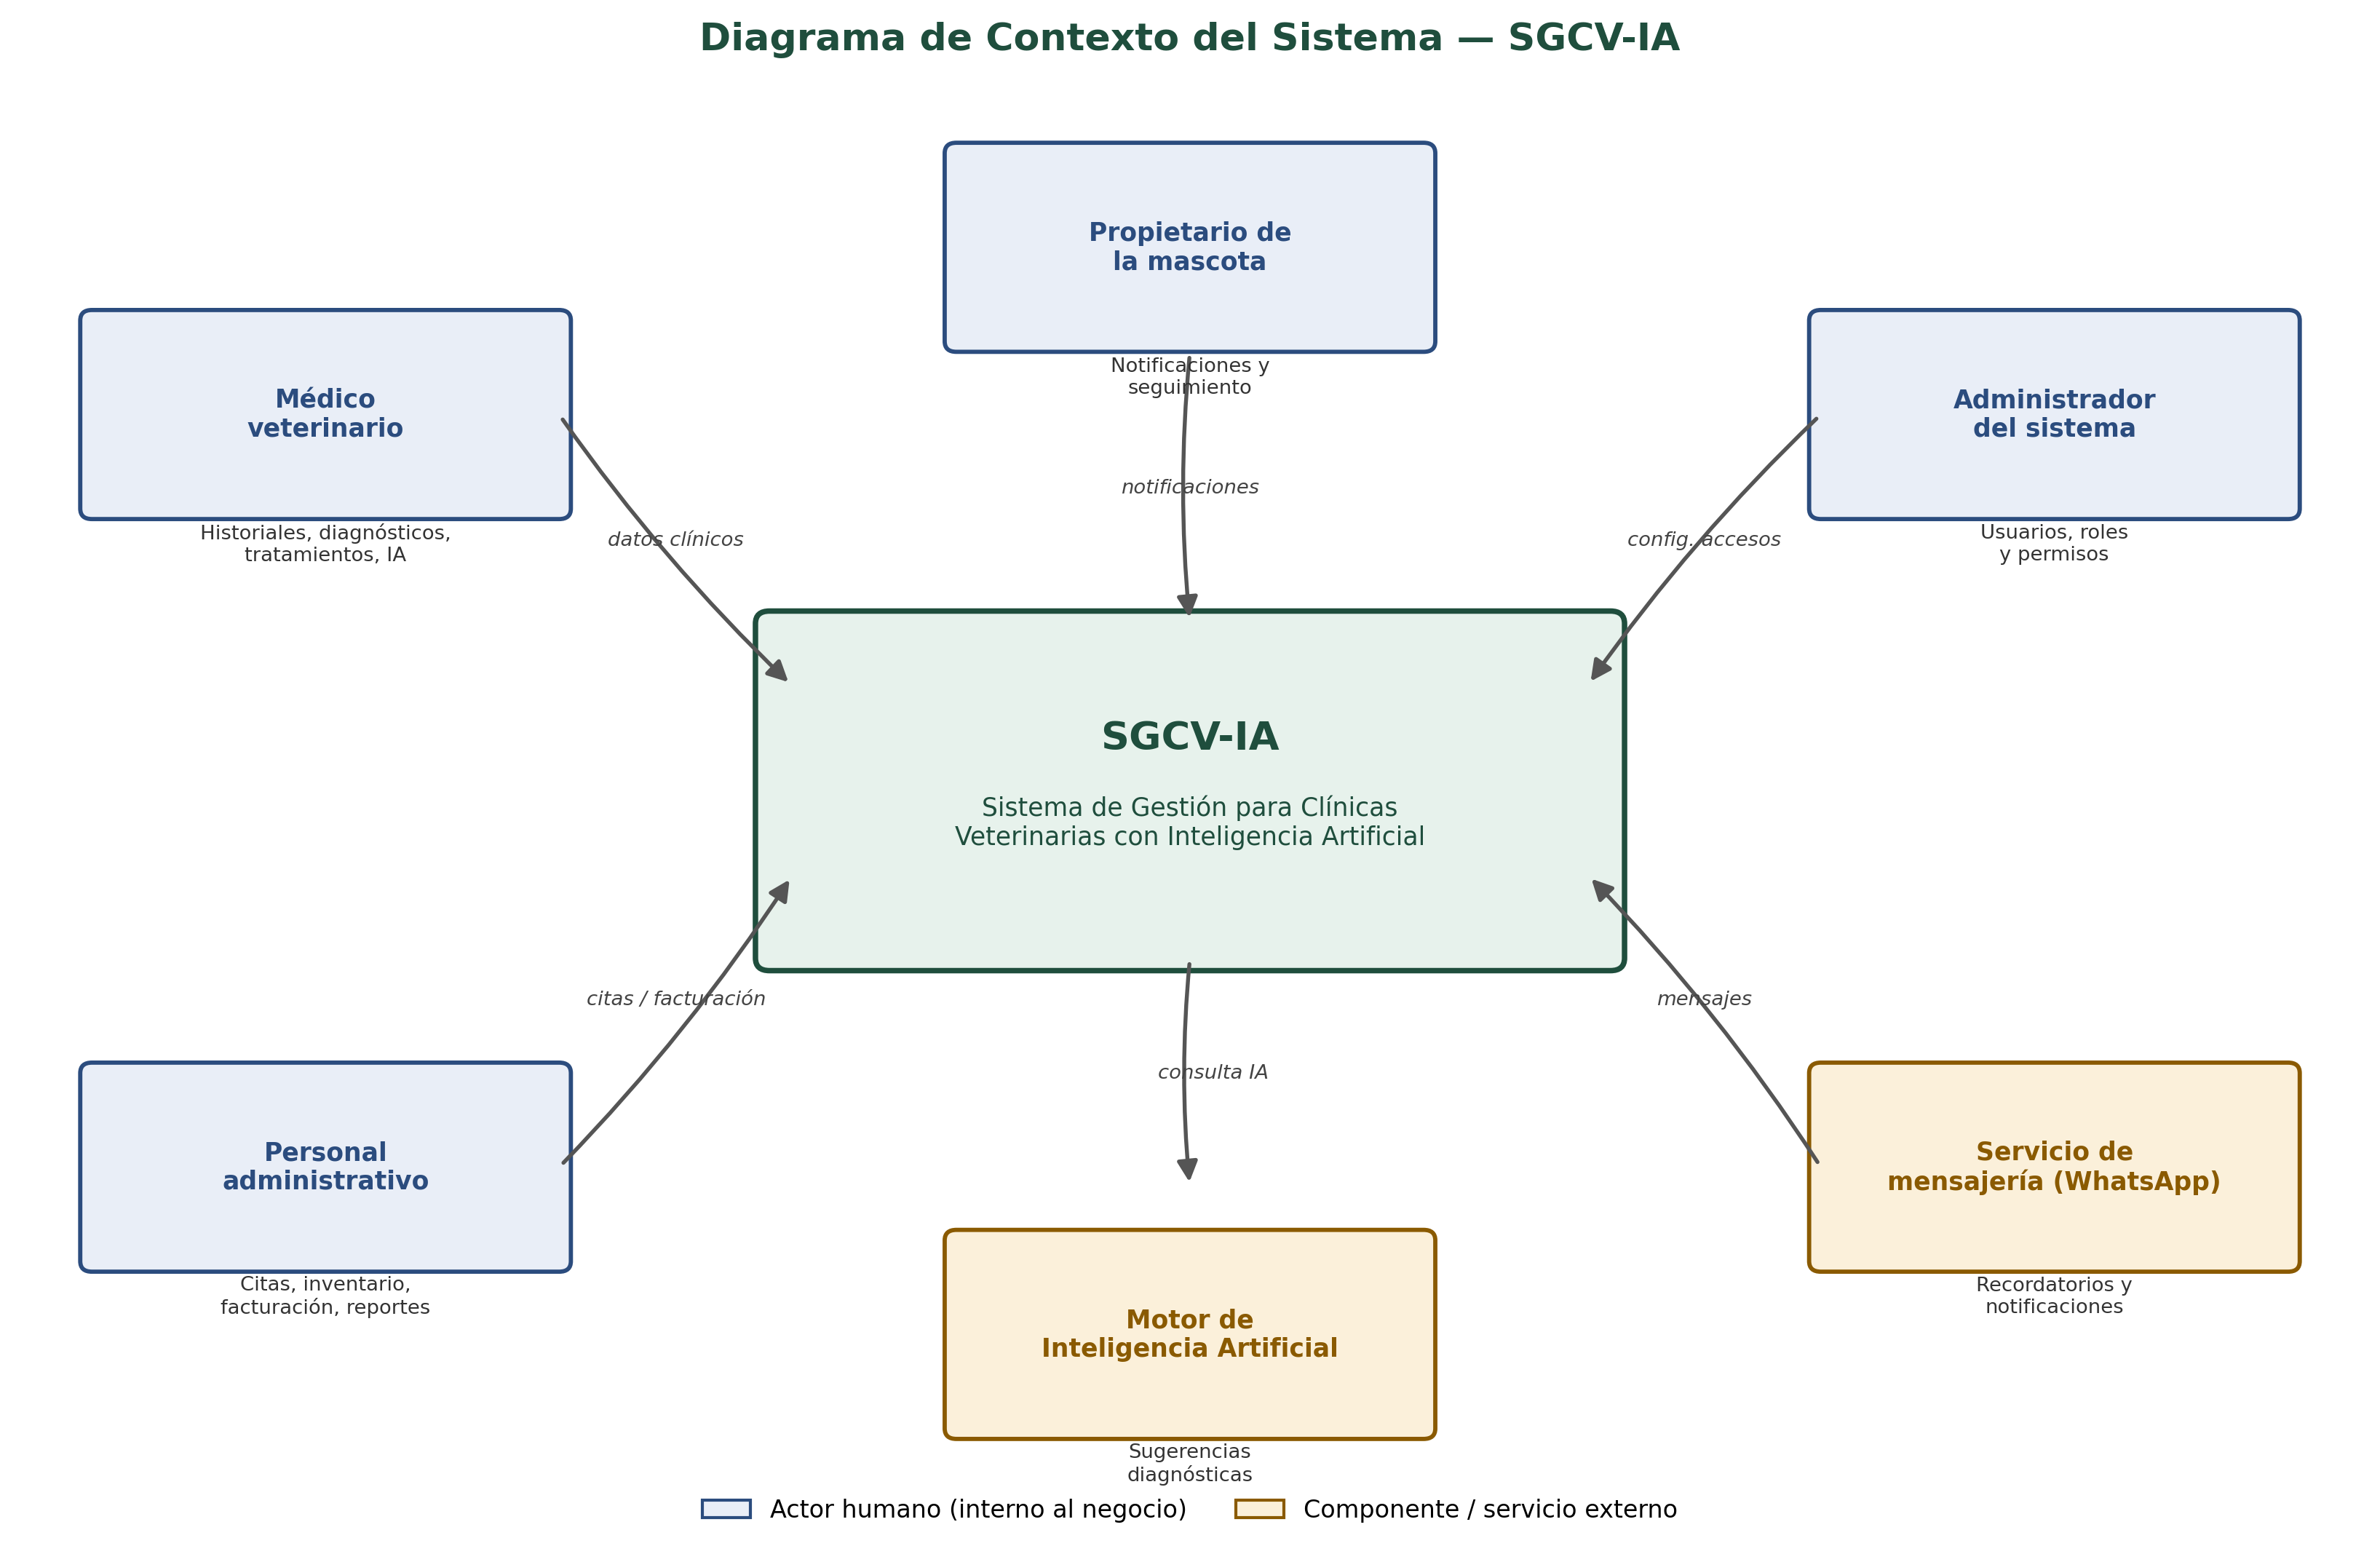
\includegraphics[width=\linewidth,keepaspectratio]{./media/Diagrama_Contexto.png}
\end{center}

\protect\phantomsection\label{_bookmark13}{}\emph{\textbf{Ilustración 1.
Diagrama de Contexto del Sistema}}

\subsection{2.3. Funciones del Producto}\label{funciones-del-producto}

\subsubsection{}\label{section}

\begin{quote}
A continuación, se presentan las principales funciones que ofrece el
SGCV-IA:
\end{quote}

{\def\LTcaptype{none} % do not increment counter
\begin{longtable}[]{@{}
  >{\centering\arraybackslash}p{(\linewidth - 4\tabcolsep) * \real{0.0530}}
  >{\raggedright\arraybackslash}p{(\linewidth - 4\tabcolsep) * \real{0.2151}}
  >{\raggedright\arraybackslash}p{(\linewidth - 4\tabcolsep) * \real{0.6880}}@{}}
\toprule\noalign{}
\begin{minipage}[b]{\linewidth}\centering
\textbf{N.°}
\end{minipage} & \begin{minipage}[b]{\linewidth}\raggedright
\textbf{Función principal}
\end{minipage} & \begin{minipage}[b]{\linewidth}\centering
\textbf{Descripción}
\end{minipage} \\
\midrule\noalign{}
\endhead
\bottomrule\noalign{}
\endlastfoot
\textbf{F1} & \begin{minipage}[t]{\linewidth}\raggedright
Gestión de historiales clínicos
\end{minipage} & \begin{minipage}[t]{\linewidth}\raggedright
Permite registrar, consultar y actualizar la información clínica de las
mascotas, incluyendo diagnósticos, tratamientos y antecedentes médicos.
\end{minipage} \\
\textbf{F2} & \begin{minipage}[t]{\linewidth}\raggedright
Control de inventario
\end{minipage} & \begin{minipage}[t]{\linewidth}\raggedright
Permite administrar el inventario de medicamentos e insumos, con alertas de productos próximos a vencer o con bajo stock.
\end{minipage} \\
\textbf{F3} & \begin{minipage}[t]{\linewidth}\raggedright
Asistente de diagnóstico con IA
\end{minipage} & \begin{minipage}[t]{\linewidth}\raggedright
Analiza la información clínica del paciente para generar sugerencias
diagnósticas que sirvan de apoyo al médico veterinario.
\end{minipage} \\
\textbf{F4} & \begin{minipage}[t]{\linewidth}\raggedright
Seguimiento nutricional
\end{minipage} & \begin{minipage}[t]{\linewidth}\raggedright
Registra el peso y otros datos del paciente para ofrecer recomendaciones nutricionales de acuerdo con sus necesidades.
\end{minipage} \\
\textbf{F5} & \begin{minipage}[t]{\linewidth}\raggedright
Gestión de citas
\end{minipage} & \begin{minipage}[t]{\linewidth}\raggedright
Permite registrar, consultar, actualizar y organizar las citas de
atención de los pacientes.
\end{minipage} \\
\textbf{F6} & \begin{minipage}[t]{\linewidth}\raggedright
Facturación
\end{minipage} & \begin{minipage}[t]{\linewidth}\raggedright
Facilita el registro de los servicios prestados y la emisión de la
factura correspondiente.
\end{minipage} \\
\textbf{F7} & \begin{minipage}[t]{\linewidth}\raggedright
Generación de reportes
\end{minipage} & \begin{minipage}[t]{\linewidth}\raggedright
Permite generar reportes relacionados con la atención clínica, el
inventario y la gestión de la clínica veterinaria.
\end{minipage} \\
\textbf{F8} & \begin{minipage}[t]{\linewidth}\raggedright
Gestión de usuarios
\end{minipage} & \begin{minipage}[t]{\linewidth}\raggedright
Administra las cuentas de los usuarios y los permisos de acceso según el rol asignado dentro del sistema.
\end{minipage} \\
\end{longtable}
}

\begin{quote}
\protect\phantomsection\label{_bookmark15}{}Tabla 4. Funciones del
Producto
\end{quote}

\subsection{2.4. Clases y características de
usuarios}\label{clases-y-caracteruxedsticas-de-usuarios}

\begin{quote}
Se identificaron los principales usuarios que interactuarán con el
SGCV-IA. Cada uno tendrá diferentes responsabilidades y niveles de
acceso según las actividades que realice dentro de la clínica
veterinaria.
\end{quote}

{\def\LTcaptype{none} % do not increment counter
\begin{longtable}[]{@{}
  >{\raggedright\arraybackslash}p{(\linewidth - 8\tabcolsep) * \real{0.1743}}
  >{\raggedright\arraybackslash}p{(\linewidth - 8\tabcolsep) * \real{0.1988}}
  >{\raggedright\arraybackslash}p{(\linewidth - 8\tabcolsep) * \real{0.3536}}
  >{\raggedright\arraybackslash}p{(\linewidth - 8\tabcolsep) * \real{0.0963}}
  >{\raggedright\arraybackslash}p{(\linewidth - 8\tabcolsep) * \real{0.1348}}@{}}
\toprule\noalign{}
\begin{minipage}[b]{\linewidth}\centering
\textbf{Tipo de usuario}
\end{minipage} & \begin{minipage}[b]{\linewidth}\raggedright
\textbf{Descripción}
\end{minipage} & \begin{minipage}[b]{\linewidth}\raggedright
\textbf{Responsabilidades principales}
\end{minipage} & \begin{minipage}[b]{\linewidth}\raggedright
\textbf{Nivel técnico}
\end{minipage} & \begin{minipage}[b]{\linewidth}\raggedright
\textbf{Frecuencia de uso}
\end{minipage} \\
\midrule\noalign{}
\endhead
\bottomrule\noalign{}
\endlastfoot
\textbf{Médico veterinario} &
\begin{minipage}[t]{\linewidth}\raggedright
Profesional encargado de la atención médica de las mascotas.
\end{minipage} & \begin{minipage}[t]{\linewidth}\raggedright
Registrar y consultar historiales clínicos, emitir diagnósticos,
registrar tratamientos, realizar el seguimiento nutricional y utilizar
el asistente de Inteligencia Artificial como apoyo en la toma de decisiones.
\end{minipage} & \begin{minipage}[t]{\linewidth}\raggedright
Medio
\end{minipage} & \begin{minipage}[t]{\linewidth}\raggedright
Diaria
\end{minipage} \\
\textbf{Personal administrativo} &
\begin{minipage}[t]{\linewidth}\raggedright
Responsable de las actividades administrativas de la clínica.
\end{minipage} & \begin{minipage}[t]{\linewidth}\raggedright
Gestionar citas, controlar el inventario de medicamentos e insumos,
registrar la facturación, administrar la información de los pacientes y generar reportes.
\end{minipage} & \begin{minipage}[t]{\linewidth}\raggedright
Básico - Medio
\end{minipage} & \begin{minipage}[t]{\linewidth}\raggedright
Diaria
\end{minipage} \\
\textbf{Administrador} & \begin{minipage}[t]{\linewidth}\raggedright
Usuario encargado de la administración general del sistema.
\end{minipage} & \begin{minipage}[t]{\linewidth}\raggedright
Gestionar usuarios y permisos de acceso, supervisar el funcionamiento
del sistema y consultar los reportes generados.
\end{minipage} & \begin{minipage}[t]{\linewidth}\raggedright
Medio
\end{minipage} & \begin{minipage}[t]{\linewidth}\raggedright
Frecuente
\end{minipage} \\
\end{longtable}
}

\begin{quote}
\protect\phantomsection\label{_bookmark17}{}\emph{\textbf{Tabla 5.
Clases y características de usuarios}}
\end{quote}

\paragraph{Características generales de los
usuarios}\label{caracteruxedsticas-generales-de-los-usuarios}

\subparagraph{Médico veterinario}\label{muxe9dico-veterinario}

\begin{itemize}
\item
  Posee conocimientos en medicina veterinaria.
\item
  Maneja herramientas informáticas a nivel básico o intermedio.
\item
  Utiliza el sistema durante la atención y seguimiento de los pacientes.
\end{itemize}

\subparagraph{Personal administrativo}\label{personal-administrativo}

\begin{itemize}
\item
  Cuenta con conocimientos básicos en el manejo de computadoras.
\item
  Utiliza el sistema para gestionar citas, inventario, facturación y
  consultas administrativas.
\item
  Hace uso del sistema de forma continua durante la jornada laboral.
\end{itemize}

\subparagraph{Administrador}\label{administrador}

\begin{itemize}
\item
  Tiene conocimientos básicos o intermedios del sistema.
\item
  Es responsable de administrar los usuarios y supervisar el
  funcionamiento general del SGCV-IA.
\item
  Accede al sistema de acuerdo con las necesidades de control y
  administración.
\end{itemize}

\subsection{2.5. Mapa de stakeholders}\label{mapa-de-stakeholders}

\begin{quote}
Para identificar el nivel de participación e influencia de los actores
involucrados en el desarrollo del SGCV-IA, se utilizó la matriz de
poder--interés de Mendelow. Esta herramienta permite definir la
estrategia de gestión más adecuada para cada stakeholder durante el
desarrollo e implementación del sistema.
\end{quote}

{\def\LTcaptype{none} % do not increment counter
\begin{longtable}[]{@{}
  >{\raggedright\arraybackslash}p{(\linewidth - 8\tabcolsep) * \real{0.2508}}
  >{\raggedright\arraybackslash}p{(\linewidth - 8\tabcolsep) * \real{0.0811}}
  >{\raggedright\arraybackslash}p{(\linewidth - 8\tabcolsep) * \real{0.0899}}
  >{\raggedright\arraybackslash}p{(\linewidth - 8\tabcolsep) * \real{0.1623}}
  >{\raggedright\arraybackslash}p{(\linewidth - 8\tabcolsep) * \real{0.3741}}@{}}
\toprule\noalign{}
\begin{minipage}[b]{\linewidth}\raggedright
\textbf{Stakeholder}
\end{minipage} & \begin{minipage}[b]{\linewidth}\raggedright
\textbf{Poder}
\end{minipage} & \begin{minipage}[b]{\linewidth}\raggedright
\textbf{Interés}
\end{minipage} & \begin{minipage}[b]{\linewidth}\raggedright
\textbf{Clasificación}
\end{minipage} & \begin{minipage}[b]{\linewidth}\raggedright
\textbf{Estrategia de gestión}
\end{minipage} \\
\midrule\noalign{}
\endhead
\bottomrule\noalign{}
\endlastfoot
\textbf{Propietario o administrador de la} \textbf{clínica} & Alto & Alto & Gestionar de cerca &
\begin{minipage}[t]{\linewidth}\raggedright
Participar en la definición de requisitos, validar funcionalidades y aprobar los avances del proyecto.
\end{minipage} \\
\textbf{Médico veterinario} & Alto & Alto & Gestionar de cerca &
\begin{minipage}[t]{\linewidth}\raggedright
Validar los procesos clínicos, el funcionamiento del asistente de IA y los historiales clínicos.
\end{minipage} \\
\textbf{Personal administrativo} & Medio & Alto & Mantener informado &
\begin{minipage}[t]{\linewidth}\raggedright
Validar los procesos relacionados con citas, inventario, facturación y reportes.
\end{minipage} \\
\textbf{Equipo de desarrollo} & Alto & Alto & Gestionar de cerca &
\begin{minipage}[t]{\linewidth}\raggedright
Planificar, desarrollar, implementar y verificar el cumplimiento de los requisitos del sistema.
\end{minipage} \\
\textbf{Docente evaluador (Mg. Gleiston Guerrero Ulloa)} & Alto & Medio
& Mantener satisfecho & \begin{minipage}[t]{\linewidth}\raggedright
Supervisar el desarrollo del proyecto y verificar el cumplimiento de los
criterios académicos establecidos.
\end{minipage} \\
\end{longtable}
}

\begin{quote}
\protect\phantomsection\label{_bookmark19}{}\emph{\textbf{Tabla 6. Mapa
Stakeholders del proyecto}}
\end{quote}

\subsection{2.6. Modelado Organizacional
i*}\label{modelado-organizacional-i}

\begin{quote}
Con el fin de representar las dependencias estratégicas entre los
actores del negocio y el sistema SGCV-IA, se elaboró el modelado
organizacional en lenguaje i*, compuesto por el Diagrama de Dependencia
Estratégica (SD) y el Diagrama de Razón Estratégica (SR), conforme al
Criterio C1 de la rúbrica de evaluación.
\end{quote}

\paragraph{Diagrama de Dependencia Estratégica
(SD)}\label{diagrama-de-dependencia-estrategica-sd}

\begin{quote}
El Diagrama SD representa las dependencias entre los actores externos
(médico veterinario, personal administrativo, propietario de la
mascota, administrador del sistema, motor de IA externo) y el sistema
SGCV-IA, mediante metas, tareas y recursos/softgoals. El médico
veterinario depende del sistema para obtener una sugerencia diagnóstica
y mantener el historial clínico actualizado; el propietario de la
mascota depende del sistema para recibir seguimiento oportuno,
condicionado al softgoal de confidencialidad de los datos; el sistema, a
su vez, depende del motor de IA externo para procesar los datos clínicos
anonimizados y generar la sugerencia diagnóstica.
\end{quote}

\begin{center}
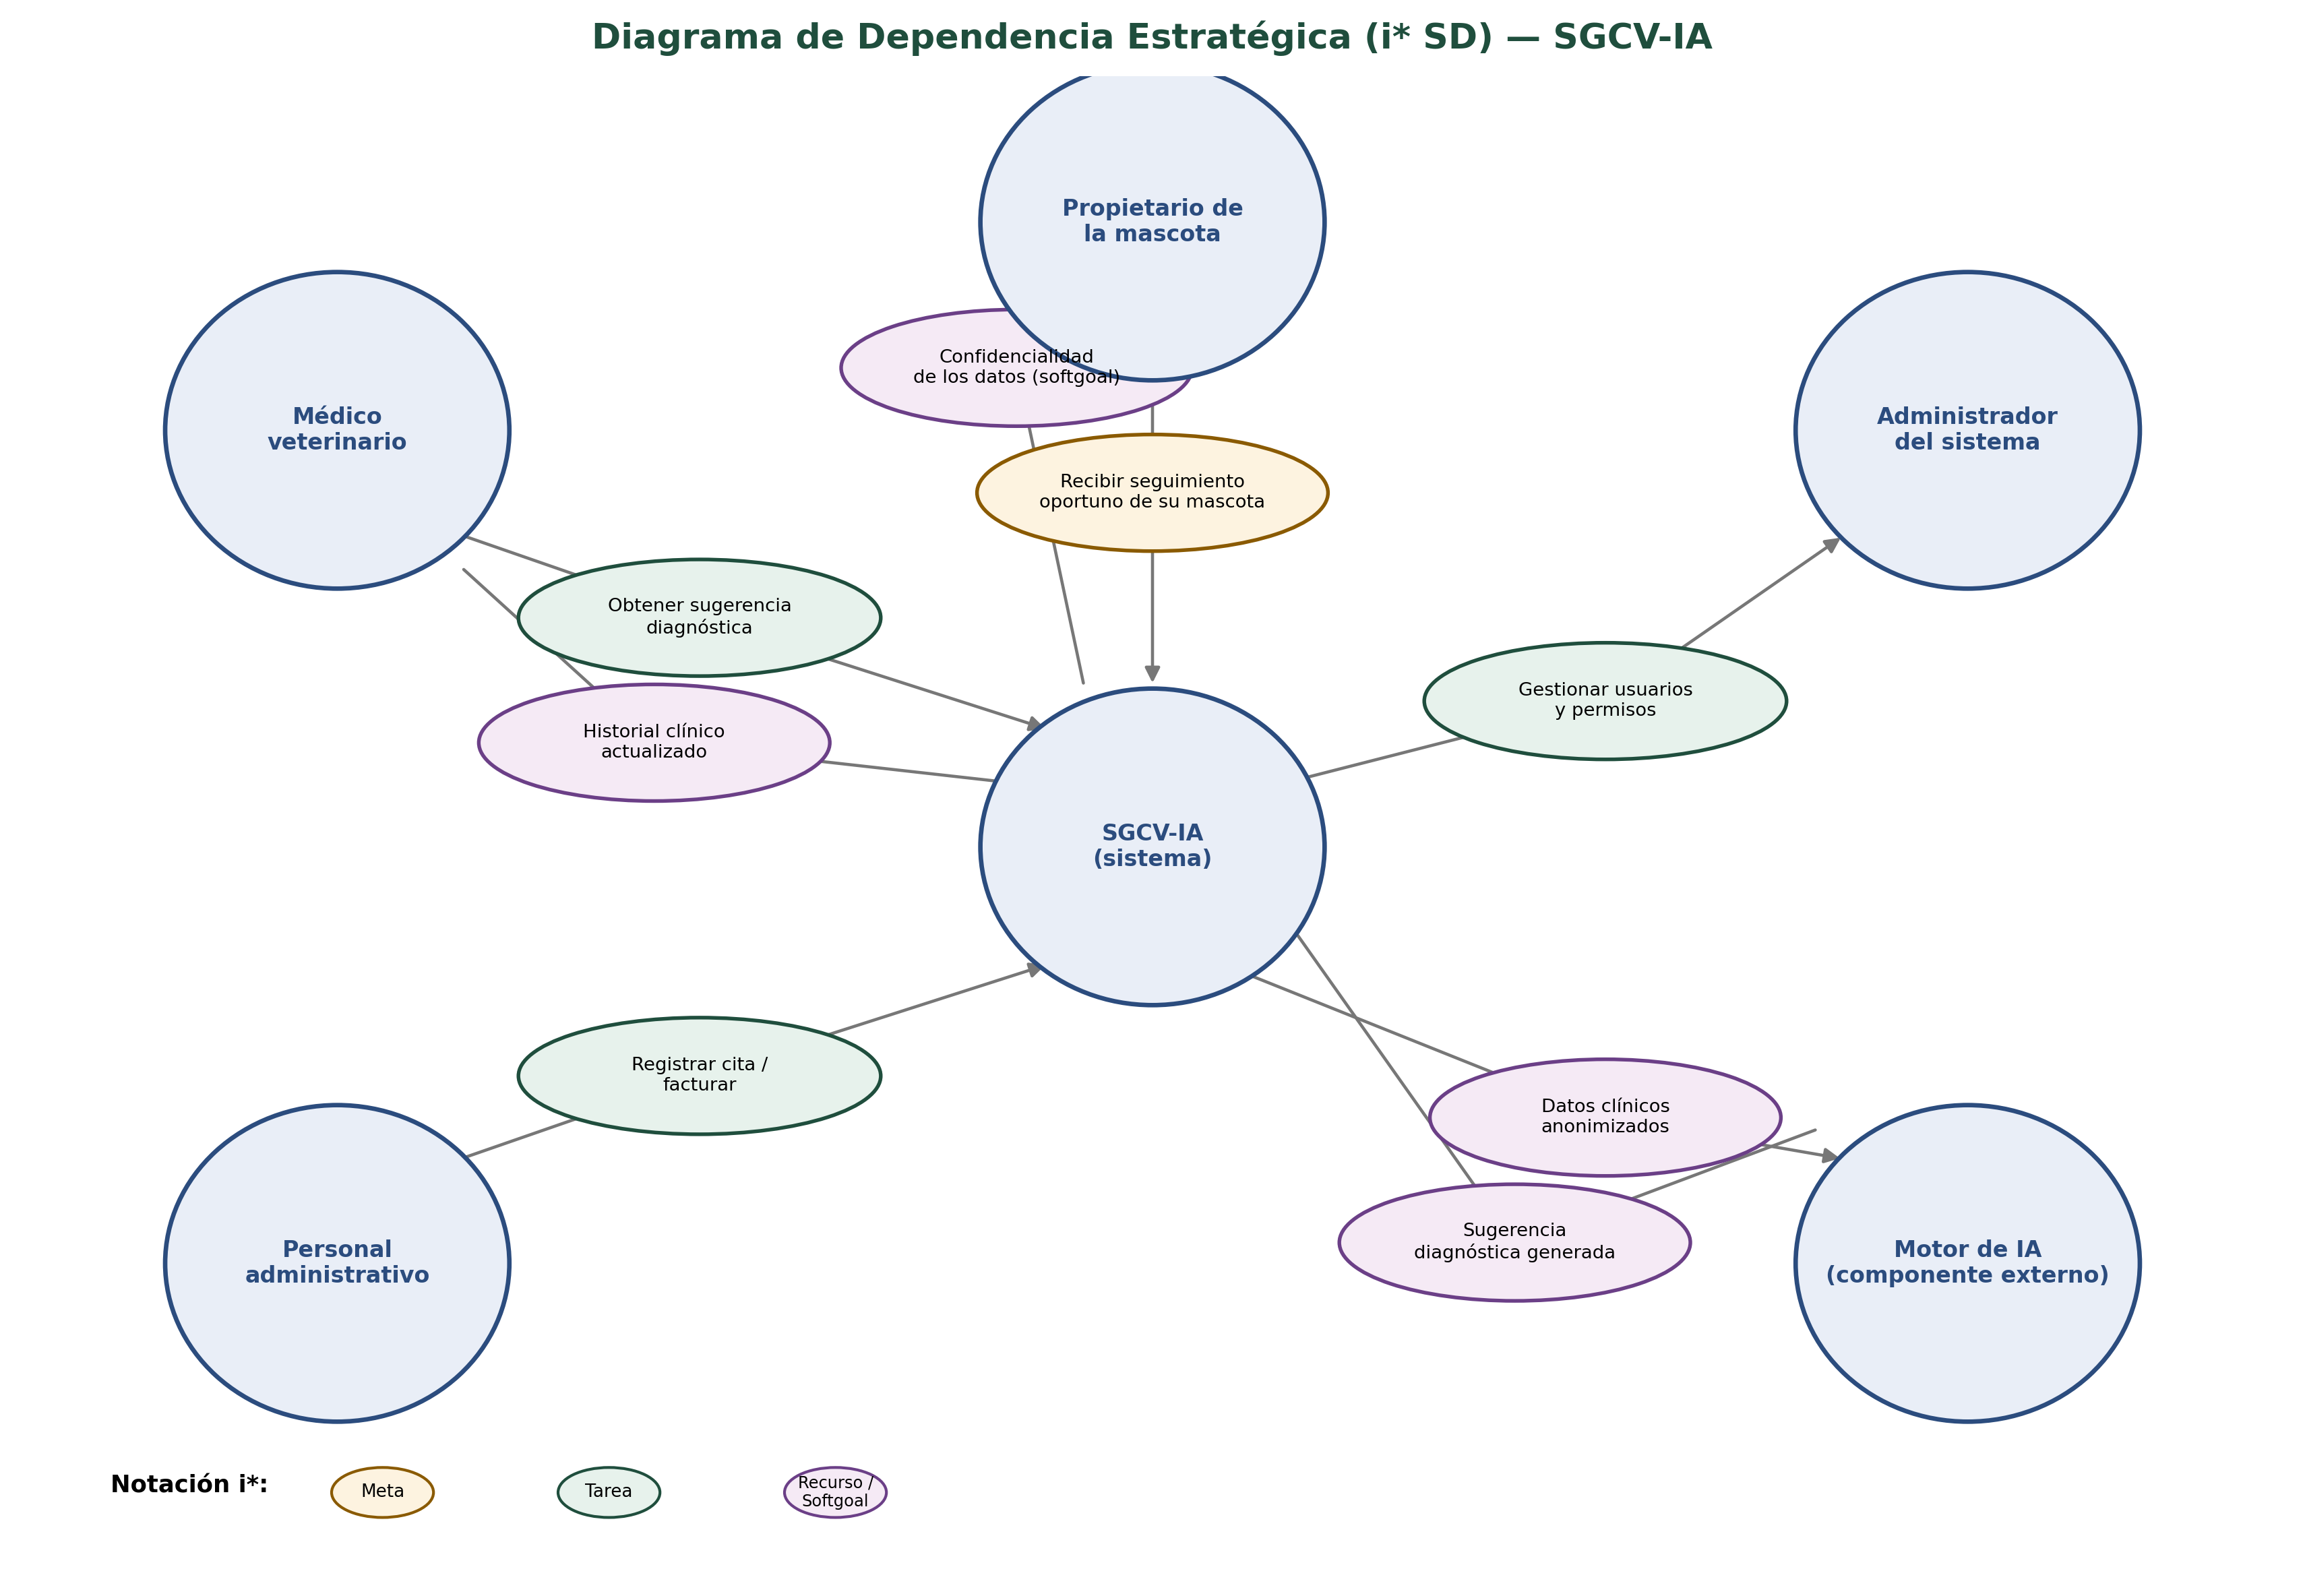
\includegraphics[width=\linewidth,keepaspectratio]{./media/iStar_SD.png}
\end{center}

\begin{quote}
\protect\phantomsection\label{_bookmark19b}{}\emph{\textbf{Ilustración 2.
Diagrama de Dependencia Estratégica (i* SD) --- SGCV-IA. Fuente:
elaboración propia (Criterio C1).}}
\end{quote}

\paragraph{Diagrama de Razón Estratégica
(SR)}\label{diagrama-de-razon-estrategica-sr}

\begin{quote}
El Diagrama SR profundiza en el razonamiento interno del actor SGCV-IA,
descomponiendo su meta principal (\emph{Apoyar la gestión integral de la
clínica}) en tres tareas: gestionar historiales clínicos, generar apoyo
diagnóstico con IA y gestionar citas, inventario y facturación. Cada
tarea se vincula a los recursos que produce o consume y a los softgoals
que condicionan su calidad: disponibilidad del historial clínico,
confiabilidad de la sugerencia diagnóstica y eficiencia en el registro
administrativo, este último dependiente del motor de IA externo para el
componente de inventario/facturación asistido.
\end{quote}

\begin{center}
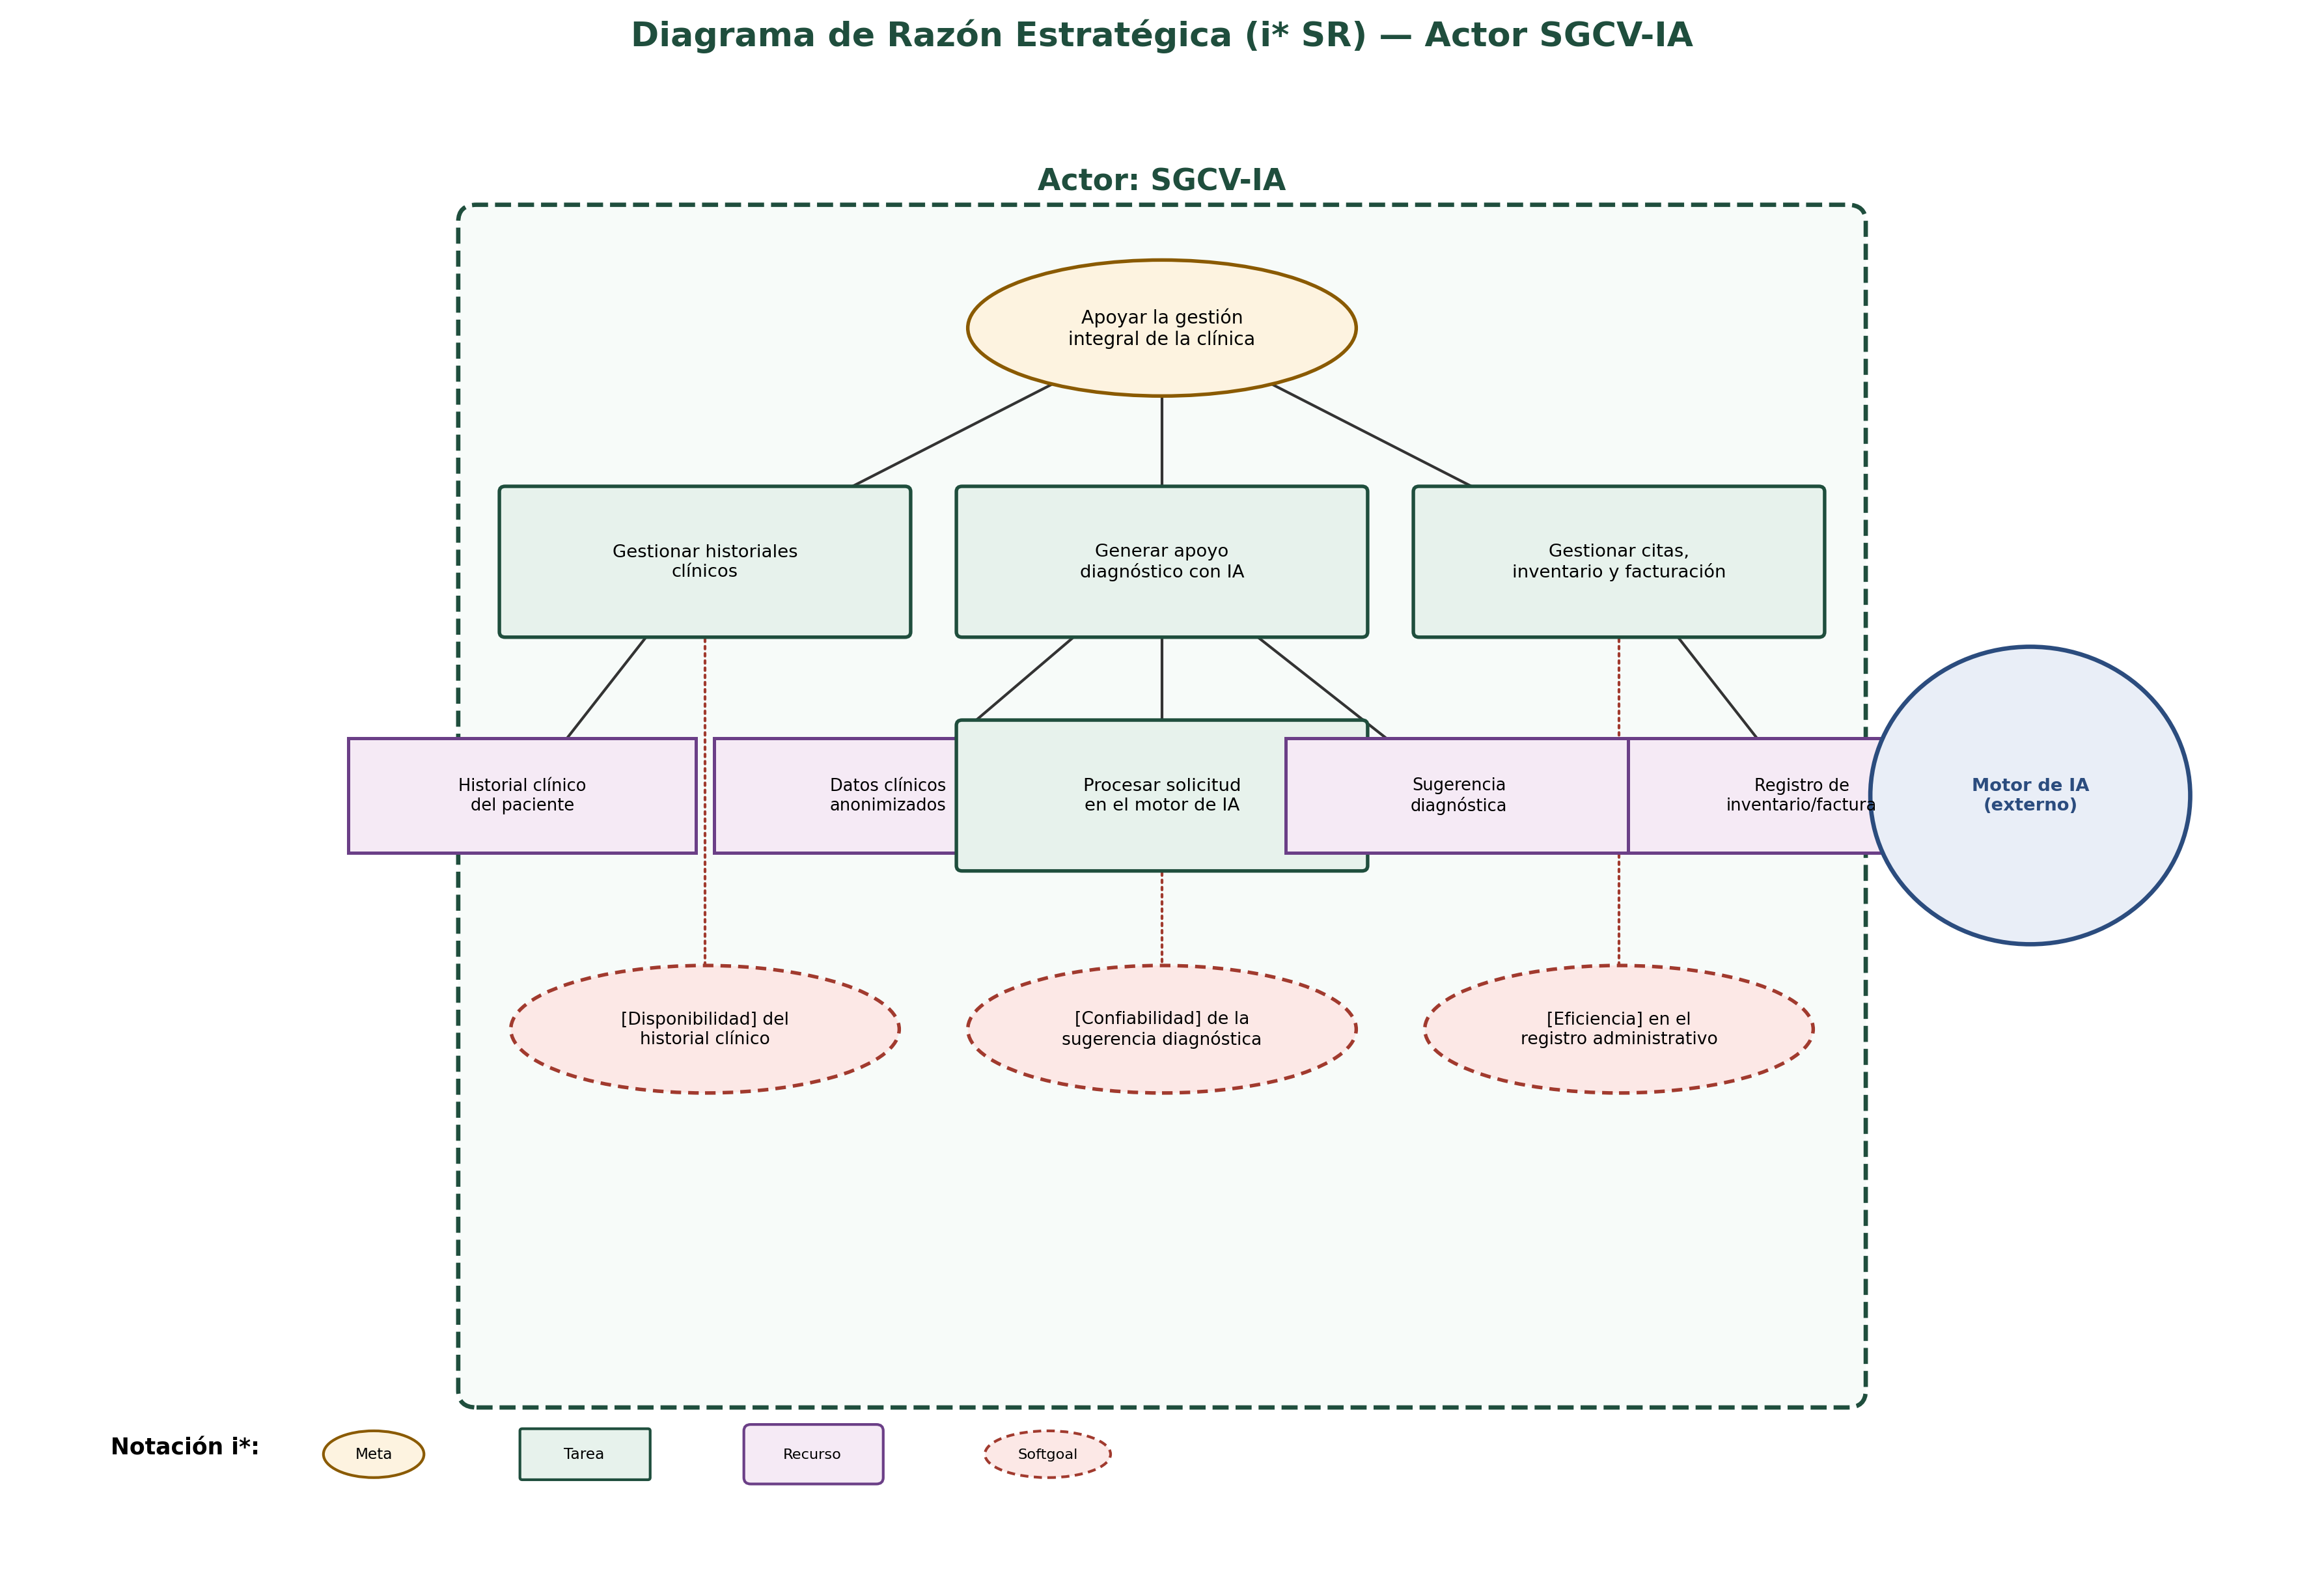
\includegraphics[width=\linewidth,keepaspectratio]{./media/iStar_SR.png}
\end{center}

\begin{quote}
\protect\phantomsection\label{_bookmark19c}{}\emph{\textbf{Ilustración 3.
Diagrama de Razón Estratégica (i* SR) --- Actor SGCV-IA. Fuente:
elaboración propia (Criterio C1).}}
\end{quote}

\subsection{2.7. Entorno operativo}\label{entorno-operativo}

\begin{quote}
l SGCV-IA será desarrollado como una aplicación web, compatible con los
principales navegadores, como \textbf{Google Chrome} (versión 100 o
superior) y \textbf{Mozilla Firefox} (versión 100 o superior). La
información del sistema se almacenará en una base de datos relacional
utilizando \textbf{MySQL}, lo que permitirá una administración segura y
organizada de los datos.
\end{quote}

\begin{itemize}
\item
  \textbf{Software:} El sistema funcionará en un servidor web y podrá
  ser utilizado desde computadoras de escritorio, portátiles y
  dispositivos móviles con acceso a un navegador web compatible.
\item
  \textbf{Conectividad:} Será necesario contar con conexión a Internet
  para acceder al sistema y utilizar todas sus funcionalidades,
  especialmente las relacionadas con el asistente de Inteligencia
  Artificial.
\item
  \textbf{Hardware:} El sistema podrá utilizarse desde computadoras de
  escritorio o portátiles para las actividades administrativas y desde
  dispositivos móviles para facilitar el acceso del médico
\end{itemize}

\begin{quote}
veterinario durante la atención de los pacientes. No requerirá equipos o
dispositivos especializados para su funcionamiento.
\end{quote}

\begin{itemize}
\item
  \textbf{Base de datos:} Toda la información clínica, administrativa y
  del inventario será almacenada en una base de datos \textbf{MySQL},
  garantizando la disponibilidad y organización de la información.
\end{itemize}

\subsection{2.8. Restricciones}\label{restricciones}

\begin{quote}
Las siguientes restricciones deberán considerarse durante el desarrollo
del SGCV-IA:
\end{quote}

\begin{itemize}
\item
  \textbf{Tecnológica:} el sistema deberá ser compatible con
  computadoras y dispositivos móviles mediante un navegador web.
\item
  \textbf{Conectividad:} será necesaria una conexión a Internet para
  utilizar todas las funcionalidades del sistema y el asistente de
  Inteligencia Artificial.
\item
  \textbf{Seguridad:} el acceso al sistema estará protegido mediante
  usuarios y permisos según el rol asignado.
\item
  \textbf{Usabilidad:} la interfaz deberá ser sencilla e intuitiva para
  facilitar su uso.
\item
  \textbf{Inteligencia Artificial:} las sugerencias generadas por la IA
  servirán únicamente como apoyo al médico veterinario y no reemplazarán
  su criterio profesional.
\end{itemize}

\subsection{2.9. Suposiciones y
Dependencias}\label{suposiciones-y-dependencias}

\paragraph{Suposiciones}\label{suposiciones}

\begin{quote}
Las siguientes suposiciones se consideran válidas durante el desarrollo
e implementación del sistema. Si cambian, los requisitos deberán
revisarse:
\end{quote}

\begin{itemize}
\item
  Se asume que los dueños de mascotas disponen de un número de teléfono
  celular activo registrado en la clínica, lo que permite el envío de
  recordatorios y resultados.
\item
  Se asume que la clínica cuenta con acceso a internet estable durante
  la mayor parte del horario de atención.
\item
  Se asume que el personal veterinario dispone de dispositivos móviles
  con sistemas operativos Android o iOS actualizados.
\item
  Se asume que el número de registros de pacientes se mantiene dentro de
  un rango manejable para la versión inicial del sistema.
\item
  Se asume la disponibilidad de datos históricos suficientes para
  alimentar y mejorar los modelos de inteligencia artificial.
\end{itemize}

\paragraph{Dependencias}\label{dependencias}

\begin{quote}
El sistema depende de los siguientes elementos externos:
\end{quote}

\begin{itemize}
\item
  Disponibilidad de conexión a internet para sincronización y acceso a
  la nube.
\item
  Disponibilidad de servicios de almacenamiento en la nube para datos
  clínicos.
\item
  Acceso a la API de WhatsApp Business o servicio equivalente para el
  envío de notificaciones.
\item
  Disponibilidad de un proveedor externo de modelos de IA (LLM) para
  funcionalidades inteligentes.
\item
  Infraestructura mínima de dispositivos móviles y/o computadoras en la
  clínica
\end{itemize}

\section{3. Requisitos Específicos}\label{requisitos-especuxedficos}

\subsection{3.1. Interfaces externas}\label{interfaces-externas}

\paragraph{Interfaz de usuario}\label{interfaz-de-usuario}

\begin{quote}
A continuación se describen las pantallas principales de la interfaz de
usuario de SGCV-IA, identificadas a partir de las funciones del producto
definidas en la Sección 2.2 y de los hallazgos de las entrevistas de
elicitación (Apéndice B). Cada pantalla se vincula con la función o
módulo que soporta; la referencia a los requisitos funcionales formales
(RF-XX) se completará en la Sección 3.2 una vez consolidada su
numeración definitiva.
\end{quote}

{\def\LTcaptype{none} % do not increment counter
\begin{longtable}[]{@{}
  >{\raggedright\arraybackslash}p{(\linewidth - 4\tabcolsep) * \real{0.2458}}
  >{\raggedright\arraybackslash}p{(\linewidth - 4\tabcolsep) * \real{0.5532}}
  >{\raggedright\arraybackslash}p{(\linewidth - 4\tabcolsep) * \real{0.1843}}@{}}
\toprule\noalign{}
\begin{minipage}[b]{\linewidth}\raggedright
\textbf{Pantalla}
\end{minipage} & \begin{minipage}[b]{\linewidth}\raggedright
\textbf{Descripción}
\end{minipage} & \begin{minipage}[b]{\linewidth}\raggedright
\textbf{Función relacionada (Sec. 2.2)}
\end{minipage} \\
\midrule\noalign{}
\endhead
\bottomrule\noalign{}
\endlastfoot
\textbf{Login / Selección de rol} &
\begin{minipage}[t]{\linewidth}\raggedright
Autenticación con usuario y contraseña; redirección al panel
correspondiente según el rol asignado (RBAC): Médico Veterinario o Personal Administrativo.
\end{minipage} & F9 \\
\textbf{Dashboard general} & \begin{minipage}[t]{\linewidth}\raggedright
Resumen del día: citas próximas, alertas de inventario por vencer o agotarse, pacientes con seguimiento pendiente y accesos rápidos
según el rol del usuario.
\end{minipage} & F1, F2, F5 \\
\textbf{Gestión de Historiales Clínicos} &
\begin{minipage}[t]{\linewidth}\raggedright
Listado de pacientes con búsqueda por nombre del animal o del dueño;
ficha de detalle con datos generales, historial de consultas, diagnósticos y tratamientos previos.
\end{minipage} & F1 \\
\textbf{Registro de Consulta} &
\begin{minipage}[t]{\linewidth}\raggedright
Formulario de nueva consulta (motivo, síntomas, diagnóstico, tratamiento, dosis y frecuencia), con acceso directo al
panel de sugerencias de IA durante el registro.
\end{minipage} & F1, F3 \\
\textbf{Panel de Diagnóstico Asistido por IA} &
\begin{minipage}[t]{\linewidth}\raggedright
Vista de los diagnósticos diferenciales sugeridos por el módulo de IA
junto con su respaldo bibliográfico; el veterinario puede aceptar,
modificar o rechazar cada sugerencia antes de registrarla.
\end{minipage} & F3 \\
\textbf{Seguimiento Nutricional} &
\begin{minipage}[t]{\linewidth}\raggedright
Registro cronológico de peso y condición corporal del paciente, con gráfico de tendencia y recomendaciones de alimentación
generadas según raza, edad y peso.
\end{minipage} & F4 \\
\textbf{Gestión de Citas y Recordatorios} &
\begin{minipage}[t]{\linewidth}\raggedright
Calendario de citas programadas por paciente, registro de
asistencia/inasistencia y configuración de recordatorios automáticos enviados al dueño.
\end{minipage} & F5 \\
\textbf{Comunicación con Dueños} &
\begin{minipage}[t]{\linewidth}\raggedright
Historial de comunicaciones (llamadas, WhatsApp) por paciente, con opción de adjuntar y enviar resultados de exámenes
directamente desde la plataforma.
\end{minipage} & F6 \\
\textbf{Facturación y Cobro} &
\begin{minipage}[t]{\linewidth}\raggedright
Formulario de cobro post-consulta en un máximo de tres pasos: selección
de servicios y productos utilizados, cálculo del monto total y emisión
del comprobante.
\end{minipage} & F7 \\
\textbf{Inventario de Bodega} &
\begin{minipage}[t]{\linewidth}\raggedright
Listado de insumos y medicamentos con stock actual y fecha de
vencimiento; formulario de entradas/salidas y panel de alertas de vencimiento próximo o stock mínimo.
\end{minipage} & F2 \\
\textbf{Reportes y Exportación} &
\begin{minipage}[t]{\linewidth}\raggedright
Generación de reportes del historial clínico y de indicadores operativos
(consultas, facturación, inventario), exportables en formato PDF para referencias a otras clínicas.
\end{minipage} & F8 \\
\end{longtable}
}

{\def\LTcaptype{none} % do not increment counter
\begin{longtable}[]{@{}
  >{\raggedright\arraybackslash}p{(\linewidth - 4\tabcolsep) * \real{0.2458}}
  >{\raggedright\arraybackslash}p{(\linewidth - 4\tabcolsep) * \real{0.5532}}
  >{\raggedright\arraybackslash}p{(\linewidth - 4\tabcolsep) * \real{0.1843}}@{}}
\toprule\noalign{}
\begin{minipage}[b]{\linewidth}\raggedright
\textbf{Gestión de Usuarios y Accesos}
\end{minipage} & \begin{minipage}[b]{\linewidth}\raggedright
Alta y edición de cuentas de personal, asignación de rol (Médico Veterinario / Personal Administrativo) y permisos de acceso a
cada módulo.
\end{minipage} & \begin{minipage}[b]{\linewidth}\raggedright
F9
\end{minipage} \\
\midrule\noalign{}
\endhead
\bottomrule\noalign{}
\endlastfoot
\end{longtable}
}

\protect\phantomsection\label{_bookmark24}{}\emph{\textbf{Tabla 7.
Interfaz de usuario}}

\begin{quote}
Los mockups de alta fidelidad correspondientes a cada pantalla fueron
desarrollados en Figma y se presentan a continuación como capturas del
prototipo; los archivos editables se incluyen en la carpeta
modelos/mockups/ del repositorio GitHub del proyecto, conforme a lo
establecido en la guía de entrega.
\end{quote}

\subparagraph{Prototipo funcional (MVP)}\label{mockups-de-interfaz-capturas-del-prototipo}

\begin{quote}
Las maquetas estáticas de Figma que documentaban el diseño de interfaz
en entregas anteriores fueron reemplazadas por el prototipo funcional
descrito en la Sección 5 (Producto Mínimo Viable). El prototipo actual
(\texttt{05\_MVP/SGCV-IA\_Prototipo\_Funcional.html}) y sus nueve
videos de demostración por pantalla
(\texttt{05\_MVP/Videos\_Demostracion/}) constituyen la referencia
vigente de interfaz de usuario, no las maquetas de Figma de versiones
previas.
\end{quote}

\paragraph{Interfaz de hardware}\label{interfaz-de-hardware}

\begin{quote}
SGCV-IA es un sistema de gestión clínica veterinaria desarrollado como
aplicación de escritorio (Windows Forms / C\#); por ello, su interfaz de
hardware se limita a los dispositivos físicos sobre los cuales se
ejecuta y con los que interactúa el personal de la clínica durante la
consulta, la facturación y la gestión de inventario. La referencia a las
funciones del producto (Sec. 2.2) se mantiene a modo orientativo, en
espera de su vinculación definitiva con los requisitos funcionales
formales (RF-XX) en la Sección 3.2.
\end{quote}

{\def\LTcaptype{none} % do not increment counter
\begin{longtable}[]{@{}
  >{\raggedright\arraybackslash}p{(\linewidth - 4\tabcolsep) * \real{0.2458}}
  >{\raggedright\arraybackslash}p{(\linewidth - 4\tabcolsep) * \real{0.5532}}
  >{\raggedright\arraybackslash}p{(\linewidth - 4\tabcolsep) * \real{0.1843}}@{}}
\toprule\noalign{}
\begin{minipage}[b]{\linewidth}\raggedright
\textbf{Componente}
\end{minipage} & \begin{minipage}[b]{\linewidth}\raggedright
\textbf{Descripción}
\end{minipage} & \begin{minipage}[b]{\linewidth}\raggedright
\textbf{Función relacionada (Sec.} \textbf{2.2)}
\end{minipage} \\
\midrule\noalign{}
\endhead
\bottomrule\noalign{}
\endlastfoot
\textbf{Equipos de cómputo cliente} &
\begin{minipage}[t]{\linewidth}\raggedright
Computadoras de escritorio o portátiles con sistema operativo Windows 10
o superior, ubicadas en recepción, consultorio y administración.
Resolución mínima de pantalla de 1366x768 píxeles, mínimo 4 GB de RAM y
conexión a la red local (LAN) de la clínica.
\end{minipage} & F1--F9 \\
\textbf{Periféricos de entrada} &
\begin{minipage}[t]{\linewidth}\raggedright
Teclado y mouse estándar para el ingreso de datos en los formularios de
historiales clínicos, consultas, facturación e inventario. No se
requiere hardware especializado adicional en el alcance actual del sistema.
\end{minipage} & F1, F3, F7 \\
\textbf{Periféricos de salida} &
\begin{minipage}[t]{\linewidth}\raggedright
Impresora local o de red (matricial o láser) conectada al equipo de
recepción/administración, utilizada para la emisión de comprobantes de
cobro y la impresión de reportes exportados en formato PDF.
\end{minipage} & F7, F8 \\
\textbf{Almacenamiento y conectividad} &
\begin{minipage}[t]{\linewidth}\raggedright
Conexión permanente, mediante red local cableada o inalámbrica, al
servidor donde reside la base de datos del sistema. No se contempla
almacenamiento local independiente en los equipos cliente más allá de la
caché temporal propia de la aplicación.
\end{minipage} & F1--F9 \\
\end{longtable}
}

\protect\phantomsection\label{table8}{}\emph{\textbf{Tabla 8.
Interfaz de hardware}}

\begin{quote}
El sistema no requiere hardware especializado adicional (lectores
biométricos, sensores u otros dispositivos IoT) en su alcance actual;
cualquier ampliación futura del hardware de soporte se documentará en
versiones posteriores del ERS.
\end{quote}

\paragraph{Interfaz de software}\label{interfaz-de-software}

\begin{quote}
A continuación, se describen los componentes de software, formatos de
intercambio e integraciones con los que interactúa SGCV-IA como
aplicación de escritorio (Windows Forms / C\#). La referencia a las
funciones del producto (Sec. 2.2) se mantiene a modo orientativo, en
espera de su vinculación definitiva con los requisitos funcionales
formales (RF-XX) en la Sección 3.2.
\end{quote}

{\def\LTcaptype{none} % do not increment counter
\begin{longtable}[]{@{}
  >{\raggedright\arraybackslash}p{(\linewidth - 4\tabcolsep) * \real{0.2458}}
  >{\raggedright\arraybackslash}p{(\linewidth - 4\tabcolsep) * \real{0.5532}}
  >{\raggedright\arraybackslash}p{(\linewidth - 4\tabcolsep) * \real{0.1843}}@{}}
\toprule\noalign{}
\begin{minipage}[b]{\linewidth}\raggedright
\textbf{Componente}
\end{minipage} & \begin{minipage}[b]{\linewidth}\raggedright
\textbf{Descripción}
\end{minipage} & \begin{minipage}[b]{\linewidth}\raggedright
\textbf{Función relacionada (Sec. 2.2)}
\end{minipage} \\
\midrule\noalign{}
\endhead
\bottomrule\noalign{}
\endlastfoot
\textbf{Sistema operativo y plataforma} &
\begin{minipage}[t]{\linewidth}\raggedright
Aplicación de escritorio desarrollada en C\# sobre el framework .NET (Windows Forms), compatible con Windows 10 o superior. No requiere
instalación de máquina virtual ni dependencias de plataformas externas
para su ejecución en el cliente.
\end{minipage} & F1--F9 \\
\textbf{Base de datos} & \begin{minipage}[t]{\linewidth}\raggedright
Motor de base de datos relacional (SQL Server o equivalente) alojado en
el servidor de la clínica, accedido mediante ADO.NET o un ORM (p. ej.
Entity Framework) a través de la red local. Almacena historiales
clínicos, citas, inventario, facturación y usuarios.
\end{minipage} & F1, F2, F5, F7, F9 \\
\textbf{Formato de intercambio de datos} &
\begin{minipage}[t]{\linewidth}\raggedright
Generación de reportes exportables en formato PDF (historial clínico,
indicadores operativos) mediante una biblioteca de generación de
documentos integrada en la aplicación. Intercambio interno de datos en formato estructurado (objetos .NET / DataSet) entre los módulos del sistema.
\end{minipage} & F8 \\
\textbf{Módulo de IA} & \begin{minipage}[t]{\linewidth}\raggedright
Comunicación con el módulo de diagnóstico asistido mediante una API
interna (REST/HTTP) que recibe los datos de la consulta (síntomas,
motivo) y devuelve los diagnósticos diferenciales sugeridos junto con su
respaldo bibliográfico.
\end{minipage} & F3 \\
\textbf{Comunicación con terceros} &
\begin{minipage}[t]{\linewidth}\raggedright
Integración con servicios externos de mensajería (p. ej. WhatsApp
Business API) y/o correo electrónico para el envío de
\end{minipage} & F5, F6 \\
\end{longtable}
}

{\def\LTcaptype{none} % do not increment counter
\begin{longtable}[]{@{}
  >{\raggedright\arraybackslash}p{(\linewidth - 4\tabcolsep) * \real{0.2458}}
  >{\raggedright\arraybackslash}p{(\linewidth - 4\tabcolsep) * \real{0.5532}}
  >{\raggedright\arraybackslash}p{(\linewidth - 4\tabcolsep) * \real{0.1843}}@{}}
\toprule\noalign{}
\begin{minipage}[b]{\linewidth}\raggedright
\end{minipage} & \begin{minipage}[b]{\linewidth}\raggedright
recordatorios de citas y resultados de exámenes a los dueños de las
mascotas.
\end{minipage} & \begin{minipage}[b]{\linewidth}\raggedright
\end{minipage} \\
\midrule\noalign{}
\endhead
\bottomrule\noalign{}
\endlastfoot
\end{longtable}
}

\subparagraph{Tabla 9. Interfaz de
software}\label{tabla-9.-interfaz-de-software}

\begin{quote}
El módulo de IA y las integraciones de comunicación con terceros se
diseñarán como componentes desacoplados del núcleo transaccional del
sistema, de forma que su eventual indisponibilidad no comprometa el
funcionamiento de los módulos clínicos y administrativos principales.
\end{quote}

\paragraph{Interfaces de
comunicación}\label{interfaces-de-comunicaciuxf3n}

\begin{quote}
\emph{Sección pendiente de elaboración.}
\end{quote}

\subsection{3.2. Requisitos Funcionales}\label{requisitos-funcionales}

\begin{quote}
A continuación, se formalizan los requisitos funcionales (RF) de
SGCV-IA: 25 derivados de los requisitos crudos (RC) identificados durante
la elicitación (Entrega 1A/1B) y organizados por área funcional, más
RF-26 y RF-27, incorporados a partir del análisis de cumplimiento legal
(criterio C4). El requisito de negocio
RC-22 ("Bajo costo de implementación y operación") no se formaliza como
RF, ya que corresponde a un criterio de adopción y se incorpora como
restricción en la Sección 3.4. RF-25 no cuenta todavía con un caso de
uso asignado en el catálogo vigente; queda marcado como pendiente de
confirmación por el equipo.
\end{quote}

\subsubsection{3.2.1. Área 1: Gestión Operativa}\label{uxe1rea-1-gestiuxf3n-operativa}

\paragraph{RF-01 --- Acceso multiplataforma (móvil y escritorio)}\label{rf-01-acceso-multiplataforma-m-vil-y-escritori}

{\def\LTcaptype{none} % do not increment counter
\begin{longtable}[]{@{}
  >{\raggedright\arraybackslash}p{(\linewidth - 2\tabcolsep) * \real{0.2455}}
  >{\raggedright\arraybackslash}p{(\linewidth - 2\tabcolsep) * \real{0.7368}}@{}}
\toprule\noalign{}
\begin{minipage}[b]{\linewidth}\raggedright
\textbf{ID}
\end{minipage} & \begin{minipage}[b]{\linewidth}\raggedright
RF-01
\end{minipage} \\
\midrule\noalign{}
\endhead
\bottomrule\noalign{}
\endlastfoot
\textbf{Nombre} & \begin{minipage}[t]{\linewidth}\raggedright
Acceso multiplataforma (móvil y escritorio)
\end{minipage} \\
\textbf{Descripción} & \begin{minipage}[t]{\linewidth}\raggedright
El sistema debe ser accesible desde smartphones (Android/iOS) y desde computadoras de escritorio mediante navegador web, manteniendo la misma funcionalidad esencial en ambos entornos.
\end{minipage} \\
\textbf{Caso de Uso} & \begin{minipage}[t]{\linewidth}\raggedright
CU-01
\end{minipage} \\
\textbf{Fuente} & \begin{minipage}[t]{\linewidth}\raggedright
RC-01 — Entrevista, bloque D3 (Amagua y el Veterinario).
\end{minipage} \\
\textbf{Entradas / Salidas} & \begin{minipage}[t]{\linewidth}\raggedright
Entrada: Credenciales de acceso desde el dispositivo. Salida: Sesión activa con menú principal.
\end{minipage} \\
\textbf{Pre / Postcondiciones} & \begin{minipage}[t]{\linewidth}\raggedright
Pre: El usuario está registrado y activo. Post: Acceso a historiales, citas y facturación sin pérdida de funcionalidad.
\end{minipage} \\
\textbf{Prioridad} & \begin{minipage}[t]{\linewidth}\raggedright
Must have
\end{minipage} \\
\textbf{Estabilidad} & \begin{minipage}[t]{\linewidth}\raggedright
Estable
\end{minipage} \\
\textbf{Criterio de aceptación} &
\begin{minipage}[t]{\linewidth}\raggedright
El usuario puede iniciar sesión y acceder a los módulos principales (historiales, citas, facturación) desde Android, iOS y escritorio, sin pérdida de funcionalidad.
\end{minipage} \\
\textbf{Dependencias} & \begin{minipage}[t]{\linewidth}\raggedright
RF-20 (Login / Selección de rol)
\end{minipage} \\
\end{longtable}
}

\subparagraph{RF-02 --- Centralización de información clínica}\label{rf-02-centralizaci-n-de-informaci-n-cl-nica}

{\def\LTcaptype{none} % do not increment counter
\begin{longtable}[]{@{}
  >{\raggedright\arraybackslash}p{(\linewidth - 2\tabcolsep) * \real{0.2455}}
  >{\raggedright\arraybackslash}p{(\linewidth - 2\tabcolsep) * \real{0.7368}}@{}}
\toprule\noalign{}
\begin{minipage}[b]{\linewidth}\raggedright
\textbf{ID}
\end{minipage} & \begin{minipage}[b]{\linewidth}\raggedright
RF-02
\end{minipage} \\
\midrule\noalign{}
\endhead
\bottomrule\noalign{}
\endlastfoot
\textbf{Nombre} & \begin{minipage}[t]{\linewidth}\raggedright
Centralización de información clínica
\end{minipage} \\
\textbf{Descripción} & \begin{minipage}[t]{\linewidth}\raggedright
El sistema debe centralizar los historiales de todos los pacientes (nombre, edad, raza, peso, diagnósticos, tratamientos) en una única base de datos consultable desde cualquier módulo autorizado.
\end{minipage} \\
\textbf{Caso de Uso} & \begin{minipage}[t]{\linewidth}\raggedright
CU-03
\end{minipage} \\
\textbf{Fuente} & \begin{minipage}[t]{\linewidth}\raggedright
RC-02 — Entrevistas A1/A2 (Amagua; el Veterinario).
\end{minipage} \\
\textbf{Entradas / Salidas} & \begin{minipage}[t]{\linewidth}\raggedright
Entrada: Datos de una nueva consulta o paciente. Salida: Historial centralizado actualizado.
\end{minipage} \\
\textbf{Pre / Postcondiciones} & \begin{minipage}[t]{\linewidth}\raggedright
Pre: Ninguna precondición especial. Post: La consulta queda recuperable sin duplicar registros.
\end{minipage} \\
\textbf{Prioridad} & \begin{minipage}[t]{\linewidth}\raggedright
Must have
\end{minipage} \\
\textbf{Estabilidad} & \begin{minipage}[t]{\linewidth}\raggedright
Estable
\end{minipage} \\
\textbf{Criterio de aceptación} &
\begin{minipage}[t]{\linewidth}\raggedright
Toda consulta nueva queda asociada al paciente correspondiente y es recuperable desde cualquier punto de acceso autorizado, sin duplicar registros.
\end{minipage} \\
\textbf{Dependencias} & \begin{minipage}[t]{\linewidth}\raggedright
RF-04
\end{minipage} \\
\end{longtable}
}

\subparagraph{RF-03 --- Búsqueda de pacientes por nombre del animal y del dueño}\label{rf-03-b-squeda-de-pacientes-por-nombre-del-ani}

{\def\LTcaptype{none} % do not increment counter
\begin{longtable}[]{@{}
  >{\raggedright\arraybackslash}p{(\linewidth - 2\tabcolsep) * \real{0.2455}}
  >{\raggedright\arraybackslash}p{(\linewidth - 2\tabcolsep) * \real{0.7368}}@{}}
\toprule\noalign{}
\begin{minipage}[b]{\linewidth}\raggedright
\textbf{ID}
\end{minipage} & \begin{minipage}[b]{\linewidth}\raggedright
RF-03
\end{minipage} \\
\midrule\noalign{}
\endhead
\bottomrule\noalign{}
\endlastfoot
\textbf{Nombre} & \begin{minipage}[t]{\linewidth}\raggedright
Búsqueda de pacientes por nombre del animal y del dueño
\end{minipage} \\
\textbf{Descripción} & \begin{minipage}[t]{\linewidth}\raggedright
El sistema debe permitir la búsqueda de pacientes por el nombre del animal y por el nombre del propietario.
\end{minipage} \\
\textbf{Caso de Uso} & \begin{minipage}[t]{\linewidth}\raggedright
CU-03
\end{minipage} \\
\textbf{Fuente} & \begin{minipage}[t]{\linewidth}\raggedright
RC-03 — Entrevista A2, Amagua (“no está bien organizado el tema de buscar por nombre y dueño”).
\end{minipage} \\
\textbf{Entradas / Salidas} & \begin{minipage}[t]{\linewidth}\raggedright
Entrada: Término de búsqueda (nombre del animal o del dueño). Salida: Lista de pacientes coincidentes.
\end{minipage} \\
\textbf{Pre / Postcondiciones} & \begin{minipage}[t]{\linewidth}\raggedright
Pre: Se ingresan al menos 2 caracteres. Post: Resultados devueltos en $\leq$2 s (RNF-01).
\end{minipage} \\
\textbf{Prioridad} & \begin{minipage}[t]{\linewidth}\raggedright
Must have
\end{minipage} \\
\textbf{Estabilidad} & \begin{minipage}[t]{\linewidth}\raggedright
Estable
\end{minipage} \\
\textbf{Criterio de aceptación} &
\begin{minipage}[t]{\linewidth}\raggedright
El sistema retorna resultados coincidentes a partir de 2 caracteres ingresados, por nombre del animal o del dueño (tiempo cuantificado en RNF-01).
\end{minipage} \\
\textbf{Dependencias} & \begin{minipage}[t]{\linewidth}\raggedright
RF-02
\end{minipage} \\
\end{longtable}
}

\subparagraph{RF-04 --- Registro detallado del historial clínico}\label{rf-04-registro-detallado-del-historial-cl-nico}

{\def\LTcaptype{none} % do not increment counter
\begin{longtable}[]{@{}
  >{\raggedright\arraybackslash}p{(\linewidth - 2\tabcolsep) * \real{0.2455}}
  >{\raggedright\arraybackslash}p{(\linewidth - 2\tabcolsep) * \real{0.7368}}@{}}
\toprule\noalign{}
\begin{minipage}[b]{\linewidth}\raggedright
\textbf{ID}
\end{minipage} & \begin{minipage}[b]{\linewidth}\raggedright
RF-04
\end{minipage} \\
\midrule\noalign{}
\endhead
\bottomrule\noalign{}
\endlastfoot
\textbf{Nombre} & \begin{minipage}[t]{\linewidth}\raggedright
Registro detallado del historial clínico
\end{minipage} \\
\textbf{Descripción} & \begin{minipage}[t]{\linewidth}\raggedright
El sistema debe registrar en cada consulta: nombre, edad, raza, peso, motivo de consulta, diagnóstico, tratamiento, dosis, frecuencia de administración y fecha.
\end{minipage} \\
\textbf{Caso de Uso} & \begin{minipage}[t]{\linewidth}\raggedright
CU-02
\end{minipage} \\
\textbf{Fuente} & \begin{minipage}[t]{\linewidth}\raggedright
RC-04 — Entrevistas A1 (Amagua) y A2 (el Veterinario).
\end{minipage} \\
\textbf{Entradas / Salidas} & \begin{minipage}[t]{\linewidth}\raggedright
Entrada: Diagnóstico, tratamiento, dosis, frecuencia y fecha. Salida: Consulta registrada y vinculada al historial.
\end{minipage} \\
\textbf{Pre / Postcondiciones} & \begin{minipage}[t]{\linewidth}\raggedright
Pre: El paciente existe en el sistema. Post: El sistema bloquea el guardado si falta un campo obligatorio.
\end{minipage} \\
\textbf{Prioridad} & \begin{minipage}[t]{\linewidth}\raggedright
Must have
\end{minipage} \\
\textbf{Estabilidad} & \begin{minipage}[t]{\linewidth}\raggedright
Estable
\end{minipage} \\
\textbf{Criterio de aceptación} &
\begin{minipage}[t]{\linewidth}\raggedright
El formulario no permite guardar si falta algún campo obligatorio (motivo, diagnóstico, tratamiento, dosis, frecuencia, fecha).
\end{minipage} \\
\textbf{Dependencias} & \begin{minipage}[t]{\linewidth}\raggedright
RF-02, RF-23
\end{minipage} \\
\end{longtable}
}

\subparagraph{RF-05 --- Alertas automáticas de vencimiento de inventario}\label{rf-05-alertas-autom-ticas-de-vencimiento-de-in}

{\def\LTcaptype{none} % do not increment counter
\begin{longtable}[]{@{}
  >{\raggedright\arraybackslash}p{(\linewidth - 2\tabcolsep) * \real{0.2455}}
  >{\raggedright\arraybackslash}p{(\linewidth - 2\tabcolsep) * \real{0.7368}}@{}}
\toprule\noalign{}
\begin{minipage}[b]{\linewidth}\raggedright
\textbf{ID}
\end{minipage} & \begin{minipage}[b]{\linewidth}\raggedright
RF-05
\end{minipage} \\
\midrule\noalign{}
\endhead
\bottomrule\noalign{}
\endlastfoot
\textbf{Nombre} & \begin{minipage}[t]{\linewidth}\raggedright
Alertas automáticas de vencimiento de inventario
\end{minipage} \\
\textbf{Descripción} & \begin{minipage}[t]{\linewidth}\raggedright
El sistema debe registrar la fecha de vencimiento de cada producto y generar alertas automáticas conforme se aproxime dicha fecha.
\end{minipage} \\
\textbf{Caso de Uso} & \begin{minipage}[t]{\linewidth}\raggedright
CU-04
\end{minipage} \\
\textbf{Fuente} & \begin{minipage}[t]{\linewidth}\raggedright
RC-05 — Entrevista A4, el Veterinario (“siempre se caducan por falta de precaución”) y Amagua.
\end{minipage} \\
\textbf{Entradas / Salidas} & \begin{minipage}[t]{\linewidth}\raggedright
Entrada: Fecha de vencimiento de cada producto. Salida: Alerta automática de vencimiento próximo.
\end{minipage} \\
\textbf{Pre / Postcondiciones} & \begin{minipage}[t]{\linewidth}\raggedright
Pre: El producto está registrado en inventario. Post: Alerta emitida según los umbrales de RNF-03.
\end{minipage} \\
\textbf{Prioridad} & \begin{minipage}[t]{\linewidth}\raggedright
Must have
\end{minipage} \\
\textbf{Estabilidad} & \begin{minipage}[t]{\linewidth}\raggedright
Estable
\end{minipage} \\
\textbf{Criterio de aceptación} &
\begin{minipage}[t]{\linewidth}\raggedright
Las alertas se generan en los umbrales y latencia definidos en RNF-03 (30, 15 y 7 días antes del vencimiento).
\end{minipage} \\
\textbf{Dependencias} & \begin{minipage}[t]{\linewidth}\raggedright
RF-06
\end{minipage} \\
\end{longtable}
}

\subparagraph{RF-06 --- Gestión de stock con alertas de faltantes}\label{rf-06-gesti-n-de-stock-con-alertas-de-faltante}

{\def\LTcaptype{none} % do not increment counter
\begin{longtable}[]{@{}
  >{\raggedright\arraybackslash}p{(\linewidth - 2\tabcolsep) * \real{0.2455}}
  >{\raggedright\arraybackslash}p{(\linewidth - 2\tabcolsep) * \real{0.7368}}@{}}
\toprule\noalign{}
\begin{minipage}[b]{\linewidth}\raggedright
\textbf{ID}
\end{minipage} & \begin{minipage}[b]{\linewidth}\raggedright
RF-06
\end{minipage} \\
\midrule\noalign{}
\endhead
\bottomrule\noalign{}
\endlastfoot
\textbf{Nombre} & \begin{minipage}[t]{\linewidth}\raggedright
Gestión de stock con alertas de faltantes
\end{minipage} \\
\textbf{Descripción} & \begin{minipage}[t]{\linewidth}\raggedright
El sistema debe registrar las cantidades en stock de cada insumo y generar una alerta cuando el nivel caiga bajo un umbral mínimo configurable por producto.
\end{minipage} \\
\textbf{Caso de Uso} & \begin{minipage}[t]{\linewidth}\raggedright
CU-04
\end{minipage} \\
\textbf{Fuente} & \begin{minipage}[t]{\linewidth}\raggedright
RC-06 — Entrevista A4 (ambas entrevistas).
\end{minipage} \\
\textbf{Entradas / Salidas} & \begin{minipage}[t]{\linewidth}\raggedright
Entrada: Cantidad en stock y umbral mínimo configurado. Salida: Alerta de stock bajo.
\end{minipage} \\
\textbf{Pre / Postcondiciones} & \begin{minipage}[t]{\linewidth}\raggedright
Pre: El umbral mínimo está configurado por producto. Post: Notificación al Bodeguero/Administrativo al cruzar el umbral.
\end{minipage} \\
\textbf{Prioridad} & \begin{minipage}[t]{\linewidth}\raggedright
Must have
\end{minipage} \\
\textbf{Estabilidad} & \begin{minipage}[t]{\linewidth}\raggedright
Estable
\end{minipage} \\
\textbf{Criterio de aceptación} &
\begin{minipage}[t]{\linewidth}\raggedright
El sistema permite configurar un umbral mínimo por insumo y notifica al Bodeguero/Administrativo al cruzarlo.
\end{minipage} \\
\textbf{Dependencias} & \begin{minipage}[t]{\linewidth}\raggedright
RF-05
\end{minipage} \\
\end{longtable}
}

\subparagraph{RF-07 --- Registro del proceso de cobro}\label{rf-07-registro-del-proceso-de-cobro}

{\def\LTcaptype{none} % do not increment counter
\begin{longtable}[]{@{}
  >{\raggedright\arraybackslash}p{(\linewidth - 2\tabcolsep) * \real{0.2455}}
  >{\raggedright\arraybackslash}p{(\linewidth - 2\tabcolsep) * \real{0.7368}}@{}}
\toprule\noalign{}
\begin{minipage}[b]{\linewidth}\raggedright
\textbf{ID}
\end{minipage} & \begin{minipage}[b]{\linewidth}\raggedright
RF-07
\end{minipage} \\
\midrule\noalign{}
\endhead
\bottomrule\noalign{}
\endlastfoot
\textbf{Nombre} & \begin{minipage}[t]{\linewidth}\raggedright
Registro del proceso de cobro
\end{minipage} \\
\textbf{Descripción} & \begin{minipage}[t]{\linewidth}\raggedright
El sistema debe permitir registrar el cobro de cada consulta, incluyendo servicios prestados, productos utilizados y monto total cobrado.
\end{minipage} \\
\textbf{Caso de Uso} & \begin{minipage}[t]{\linewidth}\raggedright
CU-10
\end{minipage} \\
\textbf{Fuente} & \begin{minipage}[t]{\linewidth}\raggedright
RC-07 — Entrevista A3, el Veterinario y Amagua (“la parte más demorada”).
\end{minipage} \\
\textbf{Entradas / Salidas} & \begin{minipage}[t]{\linewidth}\raggedright
Entrada: Servicios y productos consumidos en la consulta. Salida: Monto total calculado y comprobante.
\end{minipage} \\
\textbf{Pre / Postcondiciones} & \begin{minipage}[t]{\linewidth}\raggedright
Pre: Existe una consulta o venta abierta. Post: El comprobante queda generado y asociado a la consulta.
\end{minipage} \\
\textbf{Prioridad} & \begin{minipage}[t]{\linewidth}\raggedright
Must have
\end{minipage} \\
\textbf{Estabilidad} & \begin{minipage}[t]{\linewidth}\raggedright
Estable
\end{minipage} \\
\textbf{Criterio de aceptación} &
\begin{minipage}[t]{\linewidth}\raggedright
El sistema permite seleccionar servicios y productos y calcula automáticamente el monto total, generando un comprobante asociado.
\end{minipage} \\
\textbf{Dependencias} & \begin{minipage}[t]{\linewidth}\raggedright
RF-08
\end{minipage} \\
\end{longtable}
}

\subparagraph{RF-08 --- Módulo de facturación ágil (máximo 3 pasos)}\label{rf-08-m-dulo-de-facturaci-n-gil-m-ximo-3-pasos}

{\def\LTcaptype{none} % do not increment counter
\begin{longtable}[]{@{}
  >{\raggedright\arraybackslash}p{(\linewidth - 2\tabcolsep) * \real{0.2455}}
  >{\raggedright\arraybackslash}p{(\linewidth - 2\tabcolsep) * \real{0.7368}}@{}}
\toprule\noalign{}
\begin{minipage}[b]{\linewidth}\raggedright
\textbf{ID}
\end{minipage} & \begin{minipage}[b]{\linewidth}\raggedright
RF-08
\end{minipage} \\
\midrule\noalign{}
\endhead
\bottomrule\noalign{}
\endlastfoot
\textbf{Nombre} & \begin{minipage}[t]{\linewidth}\raggedright
Módulo de facturación ágil (máximo 3 pasos)
\end{minipage} \\
\textbf{Descripción} & \begin{minipage}[t]{\linewidth}\raggedright
El proceso de registro de una factura no debe requerir más de tres pasos desde el inicio hasta la emisión del comprobante.
\end{minipage} \\
\textbf{Caso de Uso} & \begin{minipage}[t]{\linewidth}\raggedright
CU-10
\end{minipage} \\
\textbf{Fuente} & \begin{minipage}[t]{\linewidth}\raggedright
RC-08 — Entrevista A3, Amagua (“es la parte más demorada”).
\end{minipage} \\
\textbf{Entradas / Salidas} & \begin{minipage}[t]{\linewidth}\raggedright
Entrada: Selección de servicios/productos a cobrar. Salida: Factura emitida.
\end{minipage} \\
\textbf{Pre / Postcondiciones} & \begin{minipage}[t]{\linewidth}\raggedright
Pre: Los servicios y productos están seleccionados. Post: El cobro se completa en máximo 3 pasos (RNF-02).
\end{minipage} \\
\textbf{Prioridad} & \begin{minipage}[t]{\linewidth}\raggedright
Must have
\end{minipage} \\
\textbf{Estabilidad} & \begin{minipage}[t]{\linewidth}\raggedright
Estable
\end{minipage} \\
\textbf{Criterio de aceptación} &
\begin{minipage}[t]{\linewidth}\raggedright
El flujo de cobro se completa en máximo 3 pasos; el tiempo total queda cuantificado en RNF-02.
\end{minipage} \\
\textbf{Dependencias} & \begin{minipage}[t]{\linewidth}\raggedright
RF-07
\end{minipage} \\
\end{longtable}
}

\subparagraph{RF-09 --- Registro de comunicaciones post-consulta}\label{rf-09-registro-de-comunicaciones-post-consulta}

{\def\LTcaptype{none} % do not increment counter
\begin{longtable}[]{@{}
  >{\raggedright\arraybackslash}p{(\linewidth - 2\tabcolsep) * \real{0.2455}}
  >{\raggedright\arraybackslash}p{(\linewidth - 2\tabcolsep) * \real{0.7368}}@{}}
\toprule\noalign{}
\begin{minipage}[b]{\linewidth}\raggedright
\textbf{ID}
\end{minipage} & \begin{minipage}[b]{\linewidth}\raggedright
RF-09
\end{minipage} \\
\midrule\noalign{}
\endhead
\bottomrule\noalign{}
\endlastfoot
\textbf{Nombre} & \begin{minipage}[t]{\linewidth}\raggedright
Registro de comunicaciones post-consulta
\end{minipage} \\
\textbf{Descripción} & \begin{minipage}[t]{\linewidth}\raggedright
El sistema debe registrar las comunicaciones realizadas con los dueños de las mascotas (llamada, WhatsApp, mensaje), indicando fecha y un resumen del contenido.
\end{minipage} \\
\textbf{Caso de Uso} & \begin{minipage}[t]{\linewidth}\raggedright
CU-08
\end{minipage} \\
\textbf{Fuente} & \begin{minipage}[t]{\linewidth}\raggedright
RC-09 — Entrevista A6 (ambas entrevistas).
\end{minipage} \\
\textbf{Entradas / Salidas} & \begin{minipage}[t]{\linewidth}\raggedright
Entrada: Resumen de la atención realizada. Salida: Comunicación registrada con fecha.
\end{minipage} \\
\textbf{Pre / Postcondiciones} & \begin{minipage}[t]{\linewidth}\raggedright
Pre: El paciente tiene un propietario asociado. Post: La comunicación queda visible en el historial del paciente.
\end{minipage} \\
\textbf{Prioridad} & \begin{minipage}[t]{\linewidth}\raggedright
Should have
\end{minipage} \\
\textbf{Estabilidad} & \begin{minipage}[t]{\linewidth}\raggedright
Volátil
\end{minipage} \\
\textbf{Criterio de aceptación} &
\begin{minipage}[t]{\linewidth}\raggedright
Cada comunicación registrada queda asociada al paciente correspondiente, con tipo, fecha y resumen visibles en su ficha.
\end{minipage} \\
\textbf{Dependencias} & \begin{minipage}[t]{\linewidth}\raggedright
RF-02
\end{minipage} \\
\end{longtable}
}

\subparagraph{RF-10 --- Envío de resultados de exámenes por WhatsApp}\label{rf-10-env-o-de-resultados-de-ex-menes-por-what}

{\def\LTcaptype{none} % do not increment counter
\begin{longtable}[]{@{}
  >{\raggedright\arraybackslash}p{(\linewidth - 2\tabcolsep) * \real{0.2455}}
  >{\raggedright\arraybackslash}p{(\linewidth - 2\tabcolsep) * \real{0.7368}}@{}}
\toprule\noalign{}
\begin{minipage}[b]{\linewidth}\raggedright
\textbf{ID}
\end{minipage} & \begin{minipage}[b]{\linewidth}\raggedright
RF-10
\end{minipage} \\
\midrule\noalign{}
\endhead
\bottomrule\noalign{}
\endlastfoot
\textbf{Nombre} & \begin{minipage}[t]{\linewidth}\raggedright
Envío de resultados de exámenes por WhatsApp
\end{minipage} \\
\textbf{Descripción} & \begin{minipage}[t]{\linewidth}\raggedright
El sistema debe permitir adjuntar y enviar resultados de exámenes directamente por WhatsApp desde la plataforma.
\end{minipage} \\
\textbf{Caso de Uso} & \begin{minipage}[t]{\linewidth}\raggedright
CU-08
\end{minipage} \\
\textbf{Fuente} & \begin{minipage}[t]{\linewidth}\raggedright
RC-10 — Entrevista A6, Amagua (“los resultados de exámenes se lo enviamos directamente por WhatsApp”).
\end{minipage} \\
\textbf{Entradas / Salidas} & \begin{minipage}[t]{\linewidth}\raggedright
Entrada: Archivo de resultados y número de contacto. Salida: Mensaje enviado por WhatsApp.
\end{minipage} \\
\textbf{Pre / Postcondiciones} & \begin{minipage}[t]{\linewidth}\raggedright
Pre: Existe una comunicación previa registrada (RF-09). Post: El estado de la comunicación cambia a “enviado”.
\end{minipage} \\
\textbf{Prioridad} & \begin{minipage}[t]{\linewidth}\raggedright
Should have
\end{minipage} \\
\textbf{Estabilidad} & \begin{minipage}[t]{\linewidth}\raggedright
Volátil
\end{minipage} \\
\textbf{Criterio de aceptación} &
\begin{minipage}[t]{\linewidth}\raggedright
El sistema permite adjuntar un archivo y enviarlo por WhatsApp desde la ficha del paciente, dejando registro en RF-09.
\end{minipage} \\
\textbf{Dependencias} & \begin{minipage}[t]{\linewidth}\raggedright
RF-09
\end{minipage} \\
\end{longtable}
}

\subparagraph{RF-11 --- Registro de citas y seguimiento de inasistencias}\label{rf-11-registro-de-citas-y-seguimiento-de-inasi}

{\def\LTcaptype{none} % do not increment counter
\begin{longtable}[]{@{}
  >{\raggedright\arraybackslash}p{(\linewidth - 2\tabcolsep) * \real{0.2455}}
  >{\raggedright\arraybackslash}p{(\linewidth - 2\tabcolsep) * \real{0.7368}}@{}}
\toprule\noalign{}
\begin{minipage}[b]{\linewidth}\raggedright
\textbf{ID}
\end{minipage} & \begin{minipage}[b]{\linewidth}\raggedright
RF-11
\end{minipage} \\
\midrule\noalign{}
\endhead
\bottomrule\noalign{}
\endlastfoot
\textbf{Nombre} & \begin{minipage}[t]{\linewidth}\raggedright
Registro de citas y seguimiento de inasistencias
\end{minipage} \\
\textbf{Descripción} & \begin{minipage}[t]{\linewidth}\raggedright
El sistema debe registrar las citas programadas, así como las asistencias e inasistencias.
\end{minipage} \\
\textbf{Caso de Uso} & \begin{minipage}[t]{\linewidth}\raggedright
CU-09
\end{minipage} \\
\textbf{Fuente} & \begin{minipage}[t]{\linewidth}\raggedright
RC-11 — Entrevista A5, Amagua (“no sabemos qué pasó con el paciente”).
\end{minipage} \\
\textbf{Entradas / Salidas} & \begin{minipage}[t]{\linewidth}\raggedright
Entrada: Fecha, hora y paciente a agendar. Salida: Cita programada.
\end{minipage} \\
\textbf{Pre / Postcondiciones} & \begin{minipage}[t]{\linewidth}\raggedright
Pre: El horario solicitado está disponible. Post: La cita queda en estado “programada” en la agenda.
\end{minipage} \\
\textbf{Prioridad} & \begin{minipage}[t]{\linewidth}\raggedright
Must have
\end{minipage} \\
\textbf{Estabilidad} & \begin{minipage}[t]{\linewidth}\raggedright
Estable
\end{minipage} \\
\textbf{Criterio de aceptación} &
\begin{minipage}[t]{\linewidth}\raggedright
Cada cita queda registrada con su estado (asistió/no asistió) y es consultable desde el historial de citas.
\end{minipage} \\
\textbf{Dependencias} & \begin{minipage}[t]{\linewidth}\raggedright
RF-12
\end{minipage} \\
\end{longtable}
}

\subparagraph{RF-12 --- Recordatorios automáticos de citas}\label{rf-12-recordatorios-autom-ticos-de-citas}

{\def\LTcaptype{none} % do not increment counter
\begin{longtable}[]{@{}
  >{\raggedright\arraybackslash}p{(\linewidth - 2\tabcolsep) * \real{0.2455}}
  >{\raggedright\arraybackslash}p{(\linewidth - 2\tabcolsep) * \real{0.7368}}@{}}
\toprule\noalign{}
\begin{minipage}[b]{\linewidth}\raggedright
\textbf{ID}
\end{minipage} & \begin{minipage}[b]{\linewidth}\raggedright
RF-12
\end{minipage} \\
\midrule\noalign{}
\endhead
\bottomrule\noalign{}
\endlastfoot
\textbf{Nombre} & \begin{minipage}[t]{\linewidth}\raggedright
Recordatorios automáticos de citas
\end{minipage} \\
\textbf{Descripción} & \begin{minipage}[t]{\linewidth}\raggedright
El sistema debe enviar recordatorios automáticos (WhatsApp o SMS) al dueño con 24 horas de antelación a una cita programada.
\end{minipage} \\
\textbf{Caso de Uso} & \begin{minipage}[t]{\linewidth}\raggedright
CU-09
\end{minipage} \\
\textbf{Historia de usuario} & \begin{minipage}[t]{\linewidth}\raggedright
HU-22 — Como propietario de la mascota, quiero recibir un recordatorio automático 24 horas antes de mi cita, para no olvidar la consulta programada.
\end{minipage} \\
\textbf{Fuente} & \begin{minipage}[t]{\linewidth}\raggedright
RC-12 — Entrevista A5 (Amagua) y A6 (el Veterinario).
\end{minipage} \\
\textbf{Entradas / Salidas} & \begin{minipage}[t]{\linewidth}\raggedright
Entrada: Hora programada de la cita. Salida: Recordatorio automático enviado.
\end{minipage} \\
\textbf{Pre / Postcondiciones} & \begin{minipage}[t]{\linewidth}\raggedright
Pre: La cita está programada (RF-11). Post: El recordatorio se envía 24 h antes sin intervención manual.
\end{minipage} \\
\textbf{Prioridad} & \begin{minipage}[t]{\linewidth}\raggedright
Should have
\end{minipage} \\
\textbf{Estabilidad} & \begin{minipage}[t]{\linewidth}\raggedright
Volátil
\end{minipage} \\
\textbf{Criterio de aceptación} &
\begin{minipage}[t]{\linewidth}\raggedright
El recordatorio se envía automáticamente 24 horas antes de la cita, sin intervención manual.
\end{minipage} \\
\textbf{Dependencias} & \begin{minipage}[t]{\linewidth}\raggedright
RF-11
\end{minipage} \\
\end{longtable}
}

\subparagraph{RF-25 --- Panel de reportes gerenciales y estadísticas operativas}\label{rf-25-panel-de-reportes-gerenciales-y-estad-st}

{\def\LTcaptype{none} % do not increment counter
\begin{longtable}[]{@{}
  >{\raggedright\arraybackslash}p{(\linewidth - 2\tabcolsep) * \real{0.2455}}
  >{\raggedright\arraybackslash}p{(\linewidth - 2\tabcolsep) * \real{0.7368}}@{}}
\toprule\noalign{}
\begin{minipage}[b]{\linewidth}\raggedright
\textbf{ID}
\end{minipage} & \begin{minipage}[b]{\linewidth}\raggedright
RF-25
\end{minipage} \\
\midrule\noalign{}
\endhead
\bottomrule\noalign{}
\endlastfoot
\textbf{Nombre} & \begin{minipage}[t]{\linewidth}\raggedright
Panel de reportes gerenciales y estadísticas operativas
\end{minipage} \\
\textbf{Descripción} & \begin{minipage}[t]{\linewidth}\raggedright
El sistema debe generar un panel con indicadores operativos (consultas atendidas, ingresos por facturación, productos próximos a vencer, citas incumplidas) consultable por el personal administrativo.
\end{minipage} \\
\textbf{Caso de Uso} & \begin{minipage}[t]{\linewidth}\raggedright
Transversal (fusionado — no correspondía a ninguno de los 10 CU existentes).
\end{minipage} \\
\textbf{Historia de usuario} & \begin{minipage}[t]{\linewidth}\raggedright
HU-21 — Como propietario o administrador de la clínica, quiero visualizar un panel con indicadores operativos, para tomar decisiones de gestión basadas en datos actualizados.
\end{minipage} \\
\textbf{Fuente} & \begin{minipage}[t]{\linewidth}\raggedright
SGCVIA\_RF\_RNF\_Cuantificables.docx (Entrega 1B).
\end{minipage} \\
\textbf{Entradas / Salidas} & \begin{minipage}[t]{\linewidth}\raggedright
Entrada: Período seleccionado (día, semana o mes). Salida: Panel con indicadores operativos.
\end{minipage} \\
\textbf{Pre / Postcondiciones} & \begin{minipage}[t]{\linewidth}\raggedright
Pre: Existen registros del sistema en el período seleccionado. Post: Los indicadores se muestran actualizados.
\end{minipage} \\
\textbf{Prioridad} & \begin{minipage}[t]{\linewidth}\raggedright
Could have
\end{minipage} \\
\textbf{Estabilidad} & \begin{minipage}[t]{\linewidth}\raggedright
Volátil
\end{minipage} \\
\textbf{Criterio de aceptación} &
\begin{minipage}[t]{\linewidth}\raggedright
El panel muestra los indicadores del período seleccionado (día, semana, mes) actualizados con la información registrada en el sistema.
\end{minipage} \\
\textbf{Dependencias} & \begin{minipage}[t]{\linewidth}\raggedright
—
\end{minipage} \\
\end{longtable}
}

\subsubsection{3.2.2. Área 2: Seguimiento Clínico y Nutricional}\label{area-2-seguimiento-clinico}

\subparagraph{RF-13 --- Seguimiento cronológico de peso y condición corporal}\label{rf-13-seguimiento-cronol-gico-de-peso-y-condic}

{\def\LTcaptype{none} % do not increment counter
\begin{longtable}[]{@{}
  >{\raggedright\arraybackslash}p{(\linewidth - 2\tabcolsep) * \real{0.2455}}
  >{\raggedright\arraybackslash}p{(\linewidth - 2\tabcolsep) * \real{0.7368}}@{}}
\toprule\noalign{}
\begin{minipage}[b]{\linewidth}\raggedright
\textbf{ID}
\end{minipage} & \begin{minipage}[b]{\linewidth}\raggedright
RF-13
\end{minipage} \\
\midrule\noalign{}
\endhead
\bottomrule\noalign{}
\endlastfoot
\textbf{Nombre} & \begin{minipage}[t]{\linewidth}\raggedright
Seguimiento cronológico de peso y condición corporal
\end{minipage} \\
\textbf{Descripción} & \begin{minipage}[t]{\linewidth}\raggedright
El sistema debe registrar de forma cronológica el peso, la edad y los parámetros de condición corporal del animal en cada visita, permitiendo visualizar su tendencia.
\end{minipage} \\
\textbf{Caso de Uso} & \begin{minipage}[t]{\linewidth}\raggedright
CU-07
\end{minipage} \\
\textbf{Fuente} & \begin{minipage}[t]{\linewidth}\raggedright
RC-13 — Entrevista B1, el Veterinario (“en base a la edad va a agarrar el peso”) y Amagua.
\end{minipage} \\
\textbf{Entradas / Salidas} & \begin{minipage}[t]{\linewidth}\raggedright
Entrada: Peso y condición corporal registrados en la visita. Salida: Registro de seguimiento nutricional.
\end{minipage} \\
\textbf{Pre / Postcondiciones} & \begin{minipage}[t]{\linewidth}\raggedright
Pre: El paciente cuenta con historial clínico (RF-04). Post: El registro queda disponible para RF-14.
\end{minipage} \\
\textbf{Prioridad} & \begin{minipage}[t]{\linewidth}\raggedright
Must have
\end{minipage} \\
\textbf{Estabilidad} & \begin{minipage}[t]{\linewidth}\raggedright
Estable
\end{minipage} \\
\textbf{Criterio de aceptación} &
\begin{minipage}[t]{\linewidth}\raggedright
Cada nueva visita se incorpora al historial de seguimiento y se refleja en un gráfico de tendencia de peso, en orden cronológico.
\end{minipage} \\
\textbf{Dependencias} & \begin{minipage}[t]{\linewidth}\raggedright
RF-04
\end{minipage} \\
\end{longtable}
}

\subparagraph{RF-14 --- Recomendaciones nutricionales personalizadas}\label{rf-14-recomendaciones-nutricionales-personaliz}

{\def\LTcaptype{none} % do not increment counter
\begin{longtable}[]{@{}
  >{\raggedright\arraybackslash}p{(\linewidth - 2\tabcolsep) * \real{0.2455}}
  >{\raggedright\arraybackslash}p{(\linewidth - 2\tabcolsep) * \real{0.7368}}@{}}
\toprule\noalign{}
\begin{minipage}[b]{\linewidth}\raggedright
\textbf{ID}
\end{minipage} & \begin{minipage}[b]{\linewidth}\raggedright
RF-14
\end{minipage} \\
\midrule\noalign{}
\endhead
\bottomrule\noalign{}
\endlastfoot
\textbf{Nombre} & \begin{minipage}[t]{\linewidth}\raggedright
Recomendaciones nutricionales personalizadas
\end{minipage} \\
\textbf{Descripción} & \begin{minipage}[t]{\linewidth}\raggedright
El sistema debe generar recomendaciones de alimentación a partir de la raza, edad, peso y condición de salud del animal, como apoyo al juicio del veterinario.
\end{minipage} \\
\textbf{Caso de Uso} & \begin{minipage}[t]{\linewidth}\raggedright
CU-07
\end{minipage} \\
\textbf{Historia de usuario} & \begin{minipage}[t]{\linewidth}\raggedright
HU-23 — Como médico veterinario, quiero recibir recomendaciones nutricionales automáticas basadas en el peso y condición del paciente, para orientar mejor al propietario sobre su alimentación.
\end{minipage} \\
\textbf{Fuente} & \begin{minipage}[t]{\linewidth}\raggedright
RC-14 — Entrevista B2, el Veterinario (“inculcarle al dueño del perro la alimentación nutritiva adecuada”) y Amagua.
\end{minipage} \\
\textbf{Entradas / Salidas} & \begin{minipage}[t]{\linewidth}\raggedright
Entrada: Histórico de peso del paciente. Salida: Recomendación nutricional y gráfico de tendencia.
\end{minipage} \\
\textbf{Pre / Postcondiciones} & \begin{minipage}[t]{\linewidth}\raggedright
Pre: Existe al menos un registro de peso (RF-13). Post: La recomendación se actualiza al registrarse un nuevo peso.
\end{minipage} \\
\textbf{Prioridad} & \begin{minipage}[t]{\linewidth}\raggedright
Should have
\end{minipage} \\
\textbf{Estabilidad} & \begin{minipage}[t]{\linewidth}\raggedright
Volátil
\end{minipage} \\
\textbf{Criterio de aceptación} &
\begin{minipage}[t]{\linewidth}\raggedright
La recomendación se actualiza automáticamente al registrarse un nuevo dato de peso o condición corporal (RF-13).
\end{minipage} \\
\textbf{Dependencias} & \begin{minipage}[t]{\linewidth}\raggedright
RF-13
\end{minipage} \\
\end{longtable}
}

\subparagraph{RF-15 --- Recordatorios de seguimiento de indicaciones médicas}\label{rf-15-recordatorios-de-seguimiento-de-indicaci}

{\def\LTcaptype{none} % do not increment counter
\begin{longtable}[]{@{}
  >{\raggedright\arraybackslash}p{(\linewidth - 2\tabcolsep) * \real{0.2455}}
  >{\raggedright\arraybackslash}p{(\linewidth - 2\tabcolsep) * \real{0.7368}}@{}}
\toprule\noalign{}
\begin{minipage}[b]{\linewidth}\raggedright
\textbf{ID}
\end{minipage} & \begin{minipage}[b]{\linewidth}\raggedright
RF-15
\end{minipage} \\
\midrule\noalign{}
\endhead
\bottomrule\noalign{}
\endlastfoot
\textbf{Nombre} & \begin{minipage}[t]{\linewidth}\raggedright
Recordatorios de seguimiento de indicaciones médicas
\end{minipage} \\
\textbf{Descripción} & \begin{minipage}[t]{\linewidth}\raggedright
El sistema debe permitir programar recordatorios para verificar el cumplimiento de indicaciones médicas (medicación, dieta, reposo) en fechas establecidas por el veterinario.
\end{minipage} \\
\textbf{Caso de Uso} & \begin{minipage}[t]{\linewidth}\raggedright
CU-09
\end{minipage} \\
\textbf{Historia de usuario} & \begin{minipage}[t]{\linewidth}\raggedright
HU-24 — Como médico veterinario, quiero programar recordatorios de seguimiento de indicaciones médicas, para verificar que el propietario cumpla con el tratamiento indicado.
\end{minipage} \\
\textbf{Fuente} & \begin{minipage}[t]{\linewidth}\raggedright
RC-15 — Entrevista B3, Amagua (“esperamos que lleguen; si no, no podemos saber”).
\end{minipage} \\
\textbf{Entradas / Salidas} & \begin{minipage}[t]{\linewidth}\raggedright
Entrada: Fecha e indicación médica a verificar. Salida: Recordatorio de seguimiento programado.
\end{minipage} \\
\textbf{Pre / Postcondiciones} & \begin{minipage}[t]{\linewidth}\raggedright
Pre: Existe una consulta registrada (RF-04). Post: El personal recibe la notificación en la fecha establecida.
\end{minipage} \\
\textbf{Prioridad} & \begin{minipage}[t]{\linewidth}\raggedright
Should have
\end{minipage} \\
\textbf{Estabilidad} & \begin{minipage}[t]{\linewidth}\raggedright
Volátil
\end{minipage} \\
\textbf{Criterio de aceptación} &
\begin{minipage}[t]{\linewidth}\raggedright
El veterinario puede programar un recordatorio con fecha y descripción; el sistema notifica al personal en la fecha establecida.
\end{minipage} \\
\textbf{Dependencias} & \begin{minipage}[t]{\linewidth}\raggedright
RF-04
\end{minipage} \\
\end{longtable}
}

\subparagraph{RF-16 --- Exportación de reportes de salud del paciente en PDF}\label{rf-16-exportaci-n-de-reportes-de-salud-del-pac}

{\def\LTcaptype{none} % do not increment counter
\begin{longtable}[]{@{}
  >{\raggedright\arraybackslash}p{(\linewidth - 2\tabcolsep) * \real{0.2455}}
  >{\raggedright\arraybackslash}p{(\linewidth - 2\tabcolsep) * \real{0.7368}}@{}}
\toprule\noalign{}
\begin{minipage}[b]{\linewidth}\raggedright
\textbf{ID}
\end{minipage} & \begin{minipage}[b]{\linewidth}\raggedright
RF-16
\end{minipage} \\
\midrule\noalign{}
\endhead
\bottomrule\noalign{}
\endlastfoot
\textbf{Nombre} & \begin{minipage}[t]{\linewidth}\raggedright
Exportación de reportes de salud del paciente en PDF
\end{minipage} \\
\textbf{Descripción} & \begin{minipage}[t]{\linewidth}\raggedright
El sistema debe generar y exportar reportes del historial clínico del paciente en formato PDF, para facilitar su referencia a clínicas con mayor equipamiento.
\end{minipage} \\
\textbf{Caso de Uso} & \begin{minipage}[t]{\linewidth}\raggedright
CU-03
\end{minipage} \\
\textbf{Historia de usuario} & \begin{minipage}[t]{\linewidth}\raggedright
HU-25 — Como médico veterinario, quiero exportar el historial clínico del paciente en PDF, para remitirlo a clínicas con mayor equipamiento cuando sea necesario.
\end{minipage} \\
\textbf{Fuente} & \begin{minipage}[t]{\linewidth}\raggedright
RC-16 — Entrevista B4, el Veterinario (“se le indica que hay que hacer pruebas de sangre o llevar a una clínica con todos los equipos”).
\end{minipage} \\
\textbf{Entradas / Salidas} & \begin{minipage}[t]{\linewidth}\raggedright
Entrada: Selección del historial clínico del paciente. Salida: Reporte en formato PDF.
\end{minipage} \\
\textbf{Pre / Postcondiciones} & \begin{minipage}[t]{\linewidth}\raggedright
Pre: El historial contiene datos registrados (RF-04). Post: El archivo se genera y descarga en $\leq$5 s.
\end{minipage} \\
\textbf{Prioridad} & \begin{minipage}[t]{\linewidth}\raggedright
Should have
\end{minipage} \\
\textbf{Estabilidad} & \begin{minipage}[t]{\linewidth}\raggedright
Estable
\end{minipage} \\
\textbf{Criterio de aceptación} &
\begin{minipage}[t]{\linewidth}\raggedright
El sistema genera un PDF con el historial clínico completo del paciente, descargable en menos de 5 segundos.
\end{minipage} \\
\textbf{Dependencias} & \begin{minipage}[t]{\linewidth}\raggedright
RF-04
\end{minipage} \\
\end{longtable}
}

\subsubsection{3.2.3. Área 3: Módulo de Inteligencia Artificial}\label{area-3-modulo-ia}

\begin{quote}
El diseño de este módulo se apoya en la literatura reciente sobre
aplicabilidad y ética de la inteligencia artificial en medicina
veterinaria~\cite{bouchemla2023,owens2023,coghlan2024}, así como en los
fundamentos de la informática veterinaria como disciplina~\cite{lustgarten2020}.
\end{quote}

\subparagraph{RF-17 --- Sugerencias diagnósticas asistidas por IA (con validación obligatoria)}\label{rf-17-sugerencias-diagn-sticas-asistidas-por-i}

{\def\LTcaptype{none} % do not increment counter
\begin{longtable}[]{@{}
  >{\raggedright\arraybackslash}p{(\linewidth - 2\tabcolsep) * \real{0.2455}}
  >{\raggedright\arraybackslash}p{(\linewidth - 2\tabcolsep) * \real{0.7368}}@{}}
\toprule\noalign{}
\begin{minipage}[b]{\linewidth}\raggedright
\textbf{ID}
\end{minipage} & \begin{minipage}[b]{\linewidth}\raggedright
RF-17
\end{minipage} \\
\midrule\noalign{}
\endhead
\bottomrule\noalign{}
\endlastfoot
\textbf{Nombre} & \begin{minipage}[t]{\linewidth}\raggedright
Sugerencias diagnósticas asistidas por IA (con validación obligatoria)
\end{minipage} \\
\textbf{Descripción} & \begin{minipage}[t]{\linewidth}\raggedright
El sistema debe analizar los datos clínicos ingresados por el veterinario y sugerir posibles diagnósticos diferenciales, sin que ninguna sugerencia pueda aplicarse sin revisión y aprobación explícita del veterinario.
\end{minipage} \\
\textbf{Caso de Uso} & \begin{minipage}[t]{\linewidth}\raggedright
CU-06
\end{minipage} \\
\textbf{Fuente} & \begin{minipage}[t]{\linewidth}\raggedright
RC-17 — Entrevista C2/C4, Amagua (“si tengo que dar un visto bueno antes, sí”) y el Veterinario.
\end{minipage} \\
\textbf{Entradas / Salidas} & \begin{minipage}[t]{\linewidth}\raggedright
Entrada: Datos clínicos ingresados por el veterinario. Salida: Sugerencia diagnóstica en estado “pendiente”.
\end{minipage} \\
\textbf{Pre / Postcondiciones} & \begin{minipage}[t]{\linewidth}\raggedright
Pre: La consulta cuenta con datos clínicos suficientes. Post: Ninguna sugerencia se aplica sin aprobación del veterinario (RST-05).
\end{minipage} \\
\textbf{Prioridad} & \begin{minipage}[t]{\linewidth}\raggedright
Must have
\end{minipage} \\
\textbf{Estabilidad} & \begin{minipage}[t]{\linewidth}\raggedright
Volátil
\end{minipage} \\
\textbf{Criterio de aceptación} &
\begin{minipage}[t]{\linewidth}\raggedright
Ninguna sugerencia de IA se incorpora al historial clínico sin una acción explícita de aprobación del veterinario.
\end{minipage} \\
\textbf{Dependencias} & \begin{minipage}[t]{\linewidth}\raggedright
RF-04, RF-18, RF-19
\end{minipage} \\
\end{longtable}
}

\subparagraph{RF-18 --- Respaldo bibliográfico de las sugerencias de IA}\label{rf-18-respaldo-bibliogr-fico-de-las-sugerencia}

{\def\LTcaptype{none} % do not increment counter
\begin{longtable}[]{@{}
  >{\raggedright\arraybackslash}p{(\linewidth - 2\tabcolsep) * \real{0.2455}}
  >{\raggedright\arraybackslash}p{(\linewidth - 2\tabcolsep) * \real{0.7368}}@{}}
\toprule\noalign{}
\begin{minipage}[b]{\linewidth}\raggedright
\textbf{ID}
\end{minipage} & \begin{minipage}[b]{\linewidth}\raggedright
RF-18
\end{minipage} \\
\midrule\noalign{}
\endhead
\bottomrule\noalign{}
\endlastfoot
\textbf{Nombre} & \begin{minipage}[t]{\linewidth}\raggedright
Respaldo bibliográfico de las sugerencias de IA
\end{minipage} \\
\textbf{Descripción} & \begin{minipage}[t]{\linewidth}\raggedright
Cada sugerencia generada por el módulo de IA debe indicar su fuente bibliográfica científica, para que el veterinario pueda evaluarla antes de aceptarla.
\end{minipage} \\
\textbf{Caso de Uso} & \begin{minipage}[t]{\linewidth}\raggedright
CU-06
\end{minipage} \\
\textbf{Fuente} & \begin{minipage}[t]{\linewidth}\raggedright
RC-18 — Bloque C5, ambas entrevistas (primera opción seleccionada en ambos casos).
\end{minipage} \\
\textbf{Entradas / Salidas} & \begin{minipage}[t]{\linewidth}\raggedright
Entrada: Sugerencia diagnóstica generada (RF-17). Salida: Referencia bibliográfica asociada.
\end{minipage} \\
\textbf{Pre / Postcondiciones} & \begin{minipage}[t]{\linewidth}\raggedright
Pre: La sugerencia ya fue generada. Post: La fuente es visible para el veterinario antes de decidir.
\end{minipage} \\
\textbf{Prioridad} & \begin{minipage}[t]{\linewidth}\raggedright
Must have
\end{minipage} \\
\textbf{Estabilidad} & \begin{minipage}[t]{\linewidth}\raggedright
Volátil
\end{minipage} \\
\textbf{Criterio de aceptación} &
\begin{minipage}[t]{\linewidth}\raggedright
Cada sugerencia diagnóstica incluye al menos una referencia bibliográfica científica visible para el veterinario.
\end{minipage} \\
\textbf{Dependencias} & \begin{minipage}[t]{\linewidth}\raggedright
RF-17
\end{minipage} \\
\end{longtable}
}

\subparagraph{RF-19 --- Revisión y corrección de sugerencias de IA por el veterinario}\label{rf-19-revisi-n-y-correcci-n-de-sugerencias-de-}

{\def\LTcaptype{none} % do not increment counter
\begin{longtable}[]{@{}
  >{\raggedright\arraybackslash}p{(\linewidth - 2\tabcolsep) * \real{0.2455}}
  >{\raggedright\arraybackslash}p{(\linewidth - 2\tabcolsep) * \real{0.7368}}@{}}
\toprule\noalign{}
\begin{minipage}[b]{\linewidth}\raggedright
\textbf{ID}
\end{minipage} & \begin{minipage}[b]{\linewidth}\raggedright
RF-19
\end{minipage} \\
\midrule\noalign{}
\endhead
\bottomrule\noalign{}
\endlastfoot
\textbf{Nombre} & \begin{minipage}[t]{\linewidth}\raggedright
Revisión y corrección de sugerencias de IA por el veterinario
\end{minipage} \\
\textbf{Descripción} & \begin{minipage}[t]{\linewidth}\raggedright
El sistema debe permitir al veterinario ver, modificar o rechazar cualquier sugerencia del módulo de IA antes de que sea registrada en el historial del paciente.
\end{minipage} \\
\textbf{Caso de Uso} & \begin{minipage}[t]{\linewidth}\raggedright
CU-06
\end{minipage} \\
\textbf{Fuente} & \begin{minipage}[t]{\linewidth}\raggedright
RC-19 — Bloque C5, Amagua (segunda opción) y el Veterinario.
\end{minipage} \\
\textbf{Entradas / Salidas} & \begin{minipage}[t]{\linewidth}\raggedright
Entrada: Sugerencia diagnóstica y decisión del veterinario. Salida: Sugerencia aceptada, modificada o rechazada.
\end{minipage} \\
\textbf{Pre / Postcondiciones} & \begin{minipage}[t]{\linewidth}\raggedright
Pre: La sugerencia está en estado “pendiente” (RF-17). Post: El nuevo estado queda registrado de forma trazable.
\end{minipage} \\
\textbf{Prioridad} & \begin{minipage}[t]{\linewidth}\raggedright
Must have
\end{minipage} \\
\textbf{Estabilidad} & \begin{minipage}[t]{\linewidth}\raggedright
Volátil
\end{minipage} \\
\textbf{Criterio de aceptación} &
\begin{minipage}[t]{\linewidth}\raggedright
El veterinario dispone de “aceptar”, “modificar” y “rechazar” sobre cada sugerencia individual antes de incorporarla al historial.
\end{minipage} \\
\textbf{Dependencias} & \begin{minipage}[t]{\linewidth}\raggedright
RF-17
\end{minipage} \\
\end{longtable}
}

\subsubsection{3.2.4. Área 4: Usabilidad, Acceso y Calidad del Sistema}\label{area-4-usabilidad-acceso}

\subparagraph{RF-20 --- Interfaz sencilla sin capacitación prolongada}\label{rf-20-interfaz-sencilla-sin-capacitaci-n-prolo}

{\def\LTcaptype{none} % do not increment counter
\begin{longtable}[]{@{}
  >{\raggedright\arraybackslash}p{(\linewidth - 2\tabcolsep) * \real{0.2455}}
  >{\raggedright\arraybackslash}p{(\linewidth - 2\tabcolsep) * \real{0.7368}}@{}}
\toprule\noalign{}
\begin{minipage}[b]{\linewidth}\raggedright
\textbf{ID}
\end{minipage} & \begin{minipage}[b]{\linewidth}\raggedright
RF-20
\end{minipage} \\
\midrule\noalign{}
\endhead
\bottomrule\noalign{}
\endlastfoot
\textbf{Nombre} & \begin{minipage}[t]{\linewidth}\raggedright
Interfaz sencilla sin capacitación prolongada
\end{minipage} \\
\textbf{Descripción} & \begin{minipage}[t]{\linewidth}\raggedright
El sistema debe poder ser utilizado por un veterinario con experiencia digital básica, sin necesidad de un proceso de formación mayor a 2 horas.
\end{minipage} \\
\textbf{Caso de Uso} & \begin{minipage}[t]{\linewidth}\raggedright
Transversal
\end{minipage} \\
\textbf{Fuente} & \begin{minipage}[t]{\linewidth}\raggedright
RC-20 — Entrevista D2, el Veterinario (“que sea fácil de usar”) y Amagua (“facilidad de utilizarla”).
\end{minipage} \\
\textbf{Entradas / Salidas} & \begin{minipage}[t]{\linewidth}\raggedright
Entrada: Interacción del usuario con la interfaz. Salida: Tarea completada sin asistencia externa.
\end{minipage} \\
\textbf{Pre / Postcondiciones} & \begin{minipage}[t]{\linewidth}\raggedright
Pre: El usuario tiene experiencia digital básica. Post: Registro exitoso tras una inducción de máximo 2 horas.
\end{minipage} \\
\textbf{Prioridad} & \begin{minipage}[t]{\linewidth}\raggedright
Must have
\end{minipage} \\
\textbf{Estabilidad} & \begin{minipage}[t]{\linewidth}\raggedright
Estable
\end{minipage} \\
\textbf{Criterio de aceptación} &
\begin{minipage}[t]{\linewidth}\raggedright
Un usuario con experiencia digital básica completa el registro de una consulta sin asistencia adicional, tras una inducción no mayor a 2 horas.
\end{minipage} \\
\textbf{Dependencias} & \begin{minipage}[t]{\linewidth}\raggedright
—
\end{minipage} \\
\end{longtable}
}

\subparagraph{RF-21 --- Operación local con sincronización posterior}\label{rf-21-operaci-n-local-con-sincronizaci-n-poste}

{\def\LTcaptype{none} % do not increment counter
\begin{longtable}[]{@{}
  >{\raggedright\arraybackslash}p{(\linewidth - 2\tabcolsep) * \real{0.2455}}
  >{\raggedright\arraybackslash}p{(\linewidth - 2\tabcolsep) * \real{0.7368}}@{}}
\toprule\noalign{}
\begin{minipage}[b]{\linewidth}\raggedright
\textbf{ID}
\end{minipage} & \begin{minipage}[b]{\linewidth}\raggedright
RF-21
\end{minipage} \\
\midrule\noalign{}
\endhead
\bottomrule\noalign{}
\endlastfoot
\textbf{Nombre} & \begin{minipage}[t]{\linewidth}\raggedright
Operación local con sincronización posterior
\end{minipage} \\
\textbf{Descripción} & \begin{minipage}[t]{\linewidth}\raggedright
El sistema debe permitir el registro y la consulta de historiales clínicos de manera local cuando no haya conexión a internet, sincronizando automáticamente al restablecerse la conexión.
\end{minipage} \\
\textbf{Caso de Uso} & \begin{minipage}[t]{\linewidth}\raggedright
Transversal
\end{minipage} \\
\textbf{Historia de usuario} & \begin{minipage}[t]{\linewidth}\raggedright
HU-26 — Como médico veterinario, quiero seguir registrando y consultando historiales clínicos aunque no haya conexión a internet, para no interrumpir la atención durante cortes de conectividad.
\end{minipage} \\
\textbf{Fuente} & \begin{minipage}[t]{\linewidth}\raggedright
RC-21 — Entrevista D4, el Veterinario (nivel 2-3/5 de cortes) y Amagua (cortes poco frecuentes).
\end{minipage} \\
\textbf{Entradas / Salidas} & \begin{minipage}[t]{\linewidth}\raggedright
Entrada: Operaciones realizadas sin conexión. Salida: Datos sincronizados al restablecer la conexión.
\end{minipage} \\
\textbf{Pre / Postcondiciones} & \begin{minipage}[t]{\linewidth}\raggedright
Pre: Existe una pérdida de conectividad. Post: Sincronización completa en $\leq$30 s (RNF-04).
\end{minipage} \\
\textbf{Prioridad} & \begin{minipage}[t]{\linewidth}\raggedright
Should have
\end{minipage} \\
\textbf{Estabilidad} & \begin{minipage}[t]{\linewidth}\raggedright
Estable
\end{minipage} \\
\textbf{Criterio de aceptación} &
\begin{minipage}[t]{\linewidth}\raggedright
El registro y consulta permanecen disponibles sin conexión; la sincronización se completa según RNF-04 al restablecerse la conectividad.
\end{minipage} \\
\textbf{Dependencias} & \begin{minipage}[t]{\linewidth}\raggedright
RF-02, RF-04
\end{minipage} \\
\end{longtable}
}

\subparagraph{RF-22 --- Perfiles de usuario diferenciados con control de acceso}\label{rf-22-perfiles-de-usuario-diferenciados-con-co}

{\def\LTcaptype{none} % do not increment counter
\begin{longtable}[]{@{}
  >{\raggedright\arraybackslash}p{(\linewidth - 2\tabcolsep) * \real{0.2455}}
  >{\raggedright\arraybackslash}p{(\linewidth - 2\tabcolsep) * \real{0.7368}}@{}}
\toprule\noalign{}
\begin{minipage}[b]{\linewidth}\raggedright
\textbf{ID}
\end{minipage} & \begin{minipage}[b]{\linewidth}\raggedright
RF-22
\end{minipage} \\
\midrule\noalign{}
\endhead
\bottomrule\noalign{}
\endlastfoot
\textbf{Nombre} & \begin{minipage}[t]{\linewidth}\raggedright
Perfiles de usuario diferenciados con control de acceso
\end{minipage} \\
\textbf{Descripción} & \begin{minipage}[t]{\linewidth}\raggedright
El sistema debe gestionar al menos dos tipos de perfil de usuario, médico veterinario y personal administrativo, con accesos y permisos diferenciados por rol (RBAC).
\end{minipage} \\
\textbf{Caso de Uso} & \begin{minipage}[t]{\linewidth}\raggedright
CU-01
\end{minipage} \\
\textbf{Fuente} & \begin{minipage}[t]{\linewidth}\raggedright
RC-23 — Secciones C/D de ambas entrevistas; requisito identificado por el equipo.
\end{minipage} \\
\textbf{Entradas / Salidas} & \begin{minipage}[t]{\linewidth}\raggedright
Entrada: Credenciales y rol asignado al usuario. Salida: Acceso restringido por módulo según el rol.
\end{minipage} \\
\textbf{Pre / Postcondiciones} & \begin{minipage}[t]{\linewidth}\raggedright
Pre: El usuario está autenticado (RF-24). Post: El acceso se otorga conforme a RNF-05.
\end{minipage} \\
\textbf{Prioridad} & \begin{minipage}[t]{\linewidth}\raggedright
Must have
\end{minipage} \\
\textbf{Estabilidad} & \begin{minipage}[t]{\linewidth}\raggedright
Estable
\end{minipage} \\
\textbf{Criterio de aceptación} &
\begin{minipage}[t]{\linewidth}\raggedright
El sistema restringe el acceso a cada módulo según el rol asignado al usuario autenticado, conforme a RNF-05.
\end{minipage} \\
\textbf{Dependencias} & \begin{minipage}[t]{\linewidth}\raggedright
RF-01
\end{minipage} \\
\end{longtable}
}

\subparagraph{RF-23 --- Trazabilidad de cambios en historiales clínicos}\label{rf-23-trazabilidad-de-cambios-en-historiales-c}

{\def\LTcaptype{none} % do not increment counter
\begin{longtable}[]{@{}
  >{\raggedright\arraybackslash}p{(\linewidth - 2\tabcolsep) * \real{0.2455}}
  >{\raggedright\arraybackslash}p{(\linewidth - 2\tabcolsep) * \real{0.7368}}@{}}
\toprule\noalign{}
\begin{minipage}[b]{\linewidth}\raggedright
\textbf{ID}
\end{minipage} & \begin{minipage}[b]{\linewidth}\raggedright
RF-23
\end{minipage} \\
\midrule\noalign{}
\endhead
\bottomrule\noalign{}
\endlastfoot
\textbf{Nombre} & \begin{minipage}[t]{\linewidth}\raggedright
Trazabilidad de cambios en historiales clínicos
\end{minipage} \\
\textbf{Descripción} & \begin{minipage}[t]{\linewidth}\raggedright
El sistema debe registrar automáticamente quién realizó cada modificación sobre un historial clínico, junto con la fecha y una descripción del cambio.
\end{minipage} \\
\textbf{Caso de Uso} & \begin{minipage}[t]{\linewidth}\raggedright
CU-03
\end{minipage} \\
\textbf{Historia de usuario} & \begin{minipage}[t]{\linewidth}\raggedright
HU-27 — Como administrador del sistema, quiero que cada modificación a un historial clínico quede registrada con usuario, fecha y descripción, para auditar cambios y cumplir con la trazabilidad exigida por la LOPDP.
\end{minipage} \\
\textbf{Fuente} & \begin{minipage}[t]{\linewidth}\raggedright
RC-24 — Derivado de RC-04 y RC-17, buenas prácticas de IA clínica.
\end{minipage} \\
\textbf{Entradas / Salidas} & \begin{minipage}[t]{\linewidth}\raggedright
Entrada: Modificación realizada sobre un historial clínico. Salida: Registro de auditoría (usuario, fecha, descripción).
\end{minipage} \\
\textbf{Pre / Postcondiciones} & \begin{minipage}[t]{\linewidth}\raggedright
Pre: El usuario está autorizado a modificar el historial. Post: La entrada de auditoría no admite edición ni eliminación (RNF-06).
\end{minipage} \\
\textbf{Prioridad} & \begin{minipage}[t]{\linewidth}\raggedright
Should have
\end{minipage} \\
\textbf{Estabilidad} & \begin{minipage}[t]{\linewidth}\raggedright
Estable
\end{minipage} \\
\textbf{Criterio de aceptación} &
\begin{minipage}[t]{\linewidth}\raggedright
Toda modificación genera un registro de auditoría (usuario, fecha, descripción) que no puede editarse ni eliminarse retroactivamente, conforme a RNF-06.
\end{minipage} \\
\textbf{Dependencias} & \begin{minipage}[t]{\linewidth}\raggedright
RF-04
\end{minipage} \\
\end{longtable}
}

\subparagraph{RF-24 --- Autenticación e inicio de sesión de usuarios}\label{rf-24-autenticaci-n-e-inicio-de-sesi-n-de-usua}

{\def\LTcaptype{none} % do not increment counter
\begin{longtable}[]{@{}
  >{\raggedright\arraybackslash}p{(\linewidth - 2\tabcolsep) * \real{0.2455}}
  >{\raggedright\arraybackslash}p{(\linewidth - 2\tabcolsep) * \real{0.7368}}@{}}
\toprule\noalign{}
\begin{minipage}[b]{\linewidth}\raggedright
\textbf{ID}
\end{minipage} & \begin{minipage}[b]{\linewidth}\raggedright
RF-24
\end{minipage} \\
\midrule\noalign{}
\endhead
\bottomrule\noalign{}
\endlastfoot
\textbf{Nombre} & \begin{minipage}[t]{\linewidth}\raggedright
Autenticación e inicio de sesión de usuarios
\end{minipage} \\
\textbf{Descripción} & \begin{minipage}[t]{\linewidth}\raggedright
El sistema debe permitir a cada usuario autenticarse mediante credenciales propias (usuario y contraseña) antes de acceder a cualquier módulo, derivando al perfil correspondiente (RF-22).
\end{minipage} \\
\textbf{Caso de Uso} & \begin{minipage}[t]{\linewidth}\raggedright
CU-01
\end{minipage} \\
\textbf{Historia de usuario} & \begin{minipage}[t]{\linewidth}\raggedright
HU-20 — Como usuario del sistema, quiero autenticarme con mis credenciales propias antes de acceder a cualquier módulo, para que el sistema garantice que solo personal autorizado use la información de la clínica.
\end{minipage} \\
\textbf{Fuente} & \begin{minipage}[t]{\linewidth}\raggedright
SGCVIA\_RF\_RNF\_Cuantificables.docx (Entrega 1B).
\end{minipage} \\
\textbf{Entradas / Salidas} & \begin{minipage}[t]{\linewidth}\raggedright
Entrada: Usuario y contraseña. Salida: Sesión autenticada, derivada al perfil correspondiente.
\end{minipage} \\
\textbf{Pre / Postcondiciones} & \begin{minipage}[t]{\linewidth}\raggedright
Pre: La cuenta está activa. Post: Bloqueo de la cuenta tras 5 intentos fallidos.
\end{minipage} \\
\textbf{Prioridad} & \begin{minipage}[t]{\linewidth}\raggedright
Must have
\end{minipage} \\
\textbf{Estabilidad} & \begin{minipage}[t]{\linewidth}\raggedright
Estable
\end{minipage} \\
\textbf{Criterio de aceptación} &
\begin{minipage}[t]{\linewidth}\raggedright
El sistema no permite el acceso a ningún módulo sin una sesión autenticada válida; tras 5 intentos fallidos la cuenta se bloquea, conforme a RNF-05.
\end{minipage} \\
\textbf{Dependencias} & \begin{minipage}[t]{\linewidth}\raggedright
RF-22
\end{minipage} \\
\end{longtable}
}

\subsubsection{3.2.5. Área 5: Cumplimiento Legal y Protección de Datos}\label{area-5-cumplimiento-legal}

\subparagraph{RF-26 --- Gestión de consentimiento informado}\label{rf-26-gesti-n-de-consentimiento-informado}

{\def\LTcaptype{none} % do not increment counter
\begin{longtable}[]{@{}
  >{\raggedright\arraybackslash}p{(\linewidth - 2\tabcolsep) * \real{0.2455}}
  >{\raggedright\arraybackslash}p{(\linewidth - 2\tabcolsep) * \real{0.7368}}@{}}
\toprule\noalign{}
\begin{minipage}[b]{\linewidth}\raggedright
\textbf{ID}
\end{minipage} & \begin{minipage}[b]{\linewidth}\raggedright
RF-26
\end{minipage} \\
\midrule\noalign{}
\endhead
\bottomrule\noalign{}
\endlastfoot
\textbf{Nombre} & \begin{minipage}[t]{\linewidth}\raggedright
Gestión de consentimiento informado
\end{minipage} \\
\textbf{Descripción} & \begin{minipage}[t]{\linewidth}\raggedright
El sistema debe capturar, registrar con fecha y hora, y permitir la revocación del consentimiento del propietario para el tratamiento de sus datos personales y los del paciente, conforme al Art. 7 y Art. 8 de la LOPDP.
\end{minipage} \\
\textbf{Caso de Uso} & \begin{minipage}[t]{\linewidth}\raggedright
Transversal
\end{minipage} \\
\textbf{Fuente} & \begin{minipage}[t]{\linewidth}\raggedright
RL-01 — Criterio C4, Requisitos Legales (LOPDP Art. 7, 8).
\end{minipage} \\
\textbf{Entradas / Salidas} & \begin{minipage}[t]{\linewidth}\raggedright
Entrada: Aceptación o revocación de consentimiento. Salida: Consentimiento registrado con fecha y hora.
\end{minipage} \\
\textbf{Pre / Postcondiciones} & \begin{minipage}[t]{\linewidth}\raggedright
Pre: El propietario está identificado en el sistema. Post: Ningún otro módulo se habilita sin consentimiento registrado.
\end{minipage} \\
\textbf{Prioridad} & \begin{minipage}[t]{\linewidth}\raggedright
Must have
\end{minipage} \\
\textbf{Estabilidad} & \begin{minipage}[t]{\linewidth}\raggedright
Estable
\end{minipage} \\
\textbf{Criterio de aceptación} &
\begin{minipage}[t]{\linewidth}\raggedright
El 100\% de los registros de propietarios nuevos queda asociado a un consentimiento firmado o registrado digitalmente antes de habilitarse cualquier otro módulo.
\end{minipage} \\
\textbf{Dependencias} & \begin{minipage}[t]{\linewidth}\raggedright
RF-02
\end{minipage} \\
\textbf{Nota} & \begin{minipage}[t]{\linewidth}\raggedright
En el ERS anterior este requisito estaba numerado como RF-24. Se renumera a RF-26 siguiendo C4\_Requisitos\_Legales\_SGCV-IA.docx, que lo construye como brecha nueva sobre la base de 25 RF de Entrega 1B.
\end{minipage} \\
\end{longtable}
}

\subparagraph{RF-27 --- Portal de ejercicio de derechos (acceso, rectificación, eliminación)}\label{rf-27-portal-de-ejercicio-de-derechos-acceso-r}

{\def\LTcaptype{none} % do not increment counter
\begin{longtable}[]{@{}
  >{\raggedright\arraybackslash}p{(\linewidth - 2\tabcolsep) * \real{0.2455}}
  >{\raggedright\arraybackslash}p{(\linewidth - 2\tabcolsep) * \real{0.7368}}@{}}
\toprule\noalign{}
\begin{minipage}[b]{\linewidth}\raggedright
\textbf{ID}
\end{minipage} & \begin{minipage}[b]{\linewidth}\raggedright
RF-27
\end{minipage} \\
\midrule\noalign{}
\endhead
\bottomrule\noalign{}
\endlastfoot
\textbf{Nombre} & \begin{minipage}[t]{\linewidth}\raggedright
Portal de ejercicio de derechos (acceso, rectificación, eliminación)
\end{minipage} \\
\textbf{Descripción} & \begin{minipage}[t]{\linewidth}\raggedright
El sistema debe ofrecer un mecanismo mediante el cual el propietario pueda solicitar acceso, rectificación o eliminación de sus datos personales, conforme a los Art. 13, 14 y 15 de la LOPDP.
\end{minipage} \\
\textbf{Caso de Uso} & \begin{minipage}[t]{\linewidth}\raggedright
Transversal
\end{minipage} \\
\textbf{Fuente} & \begin{minipage}[t]{\linewidth}\raggedright
RL-04, RL-05, RL-06, RL-07 — Criterio C4, Requisitos Legales (LOPDP Art. 12, 13, 14, 15).
\end{minipage} \\
\textbf{Entradas / Salidas} & \begin{minipage}[t]{\linewidth}\raggedright
Entrada: Solicitud de derecho ARCO del propietario. Salida: Respuesta del responsable del tratamiento.
\end{minipage} \\
\textbf{Pre / Postcondiciones} & \begin{minipage}[t]{\linewidth}\raggedright
Pre: La identidad de quien solicita está verificada. Post: La respuesta se emite dentro de un plazo máximo de 15 días.
\end{minipage} \\
\textbf{Prioridad} & \begin{minipage}[t]{\linewidth}\raggedright
Must have
\end{minipage} \\
\textbf{Estabilidad} & \begin{minipage}[t]{\linewidth}\raggedright
Estable
\end{minipage} \\
\textbf{Criterio de aceptación} &
\begin{minipage}[t]{\linewidth}\raggedright
Toda solicitud registrada por el titular recibe respuesta del responsable del tratamiento dentro de un plazo máximo de 15 días.
\end{minipage} \\
\textbf{Dependencias} & \begin{minipage}[t]{\linewidth}\raggedright
RF-02, RF-26
\end{minipage} \\
\textbf{Nota} & \begin{minipage}[t]{\linewidth}\raggedright
En el ERS anterior este requisito estaba numerado como RF-26. Se renumera a RF-27 siguiendo C4\_Requisitos\_Legales\_SGCV-IA.docx.
\end{minipage} \\
\end{longtable}
}


\subsection{3.3. Requisitos No Funcionales (ISO/IEC 25010)}\label{requisitos-no-funcionales-isoiec-25010}

\begin{quote}
A continuación, se formalizan los requisitos no funcionales (RNF) de
SGCV-IA, clasificados conforme al modelo de calidad ISO/IEC
25010:2023~\cite{iso25010}. Los requisitos de usabilidad (RNF-07,
RNF-15) se fundamentan además en la norma ISO 9241-11:2018 sobre
definiciones y conceptos de usabilidad~\cite{iso9241} y en los
principios clásicos de ingeniería de usabilidad~\cite{nielsen1993}. Se
formalizaron 18 RNF (RNF-01 a RNF-18):
15 de la base técnica (Entrega 1B), RNF-16 y RNF-17 incorporados por el
análisis de cumplimiento legal (criterio C4), y RNF-18 correspondiente
a la explicabilidad de las sugerencias del módulo de Inteligencia
Artificial, exigida por la rúbrica (criterio C3). El diseño de RNF-18
se fundamenta en la literatura sobre inteligencia artificial
explicable en contextos clínicos~\cite{mienye2024,jung2023,rosenbacke2024,vanvoorst2024,tun2025,ahmed2023,he2023,bulletti2024}.
\end{quote}

{\def\LTcaptype{none} % do not increment counter
\begin{longtable}[]{@{}
  >{\raggedright\arraybackslash}p{(\linewidth - 10\tabcolsep) * \real{0.08}}
  >{\raggedright\arraybackslash}p{(\linewidth - 10\tabcolsep) * \real{0.16}}
  >{\raggedright\arraybackslash}p{(\linewidth - 10\tabcolsep) * \real{0.27}}
  >{\raggedright\arraybackslash}p{(\linewidth - 10\tabcolsep) * \real{0.27}}
  >{\raggedright\arraybackslash}p{(\linewidth - 10\tabcolsep) * \real{0.10}}
  >{\raggedright\arraybackslash}p{(\linewidth - 10\tabcolsep) * \real{0.12}}@{}}
\toprule\noalign{}
\begin{minipage}[b]{\linewidth}\raggedright
\textbf{ID}
\end{minipage} & \begin{minipage}[b]{\linewidth}\raggedright
\textbf{Característica ISO/IEC 25010}
\end{minipage} & \begin{minipage}[b]{\linewidth}\raggedright
\textbf{Requisito No Funcional}
\end{minipage} & \begin{minipage}[b]{\linewidth}\raggedright
\textbf{Métrica / Criterio de aceptación}
\end{minipage} & \begin{minipage}[b]{\linewidth}\raggedright
\textbf{CU}
\end{minipage} & \begin{minipage}[b]{\linewidth}\raggedright
\textbf{RC/RL relacionado}
\end{minipage} \\
\midrule\noalign{}
\endhead
\bottomrule\noalign{}
\endlastfoot
\textbf{RNF-01} & Eficiencia de desempeño (Tiempo de respuesta) & El sistema debe responder con rapidez a las búsquedas de pacientes por nombre del animal o del dueño. & $\leq$2 s en el 95\% de las búsquedas, sobre hasta 500 pacientes activos. & CU-03 & RC-03 \\
\textbf{RNF-02} & Eficiencia de desempeño (Comportamiento temporal) & El registro de una factura debe completarse de forma ágil, sin pasos innecesarios. & No debe exceder 3 pasos ni 90 segundos desde el inicio hasta la emisión. & CU-10 & RC-08 \\
\textbf{RNF-03} & Fiabilidad (Madurez) & El sistema debe generar alertas de vencimiento de productos de forma automática y oportuna. & Cobertura 100\%; alertas en umbrales de 30, 15 y 7 días; latencia máxima 24h. & CU-04 & RC-05 \\
\textbf{RNF-04} & Fiabilidad (Disponibilidad) & El sistema debe permitir registro y consulta de historiales de forma local ante cortes de conectividad, sincronizando al reconectar. & Disponibilidad de funciones críticas $\geq$99\%; sincronización completa en $\leq$30 s tras reconectar. & CU-03 & RC-21 \\
\textbf{RNF-05} & Seguridad (Control de acceso / Confidencialidad) & El sistema debe restringir el acceso a la información según el perfil del usuario. & 100\% de operaciones sensibles requieren autenticación; $\geq$2 perfiles; bloqueo tras 5 intentos fallidos. & CU-01 & RC-23 \\
\textbf{RNF-06} & Seguridad (Trazabilidad / No repudio) & El sistema debe registrar todos los cambios realizados sobre los historiales clínicos. & 100\% de modificaciones quedan registradas, sin edición o eliminación retroactiva. & CU-03 & RC-24 \\
\textbf{RNF-07} & Usabilidad (Capacidad de aprendizaje) & El sistema debe poder ser utilizado por personal con experiencia digital básica sin formación prolongada. & Capacitación $\leq$2h; tasa de error $\leq$5\% en las primeras 10 ejecuciones. & Transversal & RC-20 \\
\textbf{RNF-08} & Compatibilidad (Coexistencia / Portabilidad) & El sistema debe ser accesible y funcional desde múltiples dispositivos y plataformas. & Navegadores actualizados + Android 10+/iOS 14+; paridad de funciones $\geq$95\%. & Transversal & RC-01 \\
\textbf{RNF-09} & Fiabilidad / Adecuación funcional (Exactitud IA) & Las sugerencias del módulo de IA deben estar respaldadas científicamente y ser revisables antes de aplicarse. & 100\% con referencia bibliográfica y aprobación explícita; generación $\leq$5 segundos. & CU-06 & RC-17, RC-18, RC-19 \\
\textbf{RNF-10} & Mantenibilidad (Modularidad) & Una falla del proveedor externo de IA (LLM) no debe afectar la disponibilidad de los módulos restantes. & Disponibilidad de módulos no dependientes de IA $\geq$99\% ante caída total del servicio externo. & CU-06 & Sección 2.5 \\
\textbf{RNF-11} & Eficiencia (Utilización de recursos) & El sistema debe operar dentro de límites razonables de consumo de recursos, incluso bajo carga concurrente. & CPU $\leq$70\% y memoria $\leq$75\% del backend con hasta 20 usuarios concurrentes. & Transversal & Elaboración propia \\
\textbf{RNF-12} & Seguridad (Confidencialidad / Cifrado) & La información sensible debe protegerse frente a accesos no autorizados en tránsito y almacenamiento. & 100\% de datos sensibles cifrados (TLS 1.2+ en tránsito, AES-256 en reposo); contraseñas con hash + salt. & Transversal & Elaboración propia \\
\textbf{RNF-13} & Fiabilidad (Recuperabilidad) & El sistema debe permitir recuperar información ante fallos de hardware, corrupción o eliminaciones accidentales. & Backups diarios, retención $\geq$30 días; RTO $\leq$4h; RPO $\leq$24h. & Transversal & Elaboración propia \\
\textbf{RNF-14} & Mantenibilidad (Capacidad de prueba) & El sistema debe facilitar la verificación de su correcto funcionamiento ante cambios o nuevas versiones. & Cobertura de pruebas automatizadas $\geq$70\% en módulos críticos; despliegue $\leq$30 min sin interrupción. & Transversal & Elaboración propia \\
\textbf{RNF-15} & Usabilidad (Satisfacción del usuario) & El sistema debe generar una experiencia de uso satisfactoria para el personal veterinario y administrativo. & Satisfacción $\geq$80\% (SUS) tras el primer mes de uso, muestra de al menos 5 usuarios. & Transversal & Elaboración propia \\
\textbf{RNF-16} & Fiabilidad (Conservación y eliminación segura de datos) & El sistema debe aplicar políticas de retención definidas por tipo de dato y eliminar o anonimizar de forma irreversible los datos personales al vencer su plazo de conservación. & 100\% de los registros con plazo vencido son eliminados o anonimizados en un ciclo de depuración automática $\leq$30 días tras el vencimiento. & Transversal & RL-03 (Art. 10 lit. i) \\
\textbf{RNF-17} & Seguridad (Notificación de vulneraciones) & El sistema y el equipo responsable deben contar con un procedimiento documentado para detectar, registrar y notificar vulneraciones de seguridad de datos personales. & Notificación a la Autoridad $\leq$5 días y al titular $\leq$3 días desde la detección del incidente, conforme al Art. 43 y 46 de la LOPDP. & Transversal & RL-13 (Art. 43, 46) \\
\textbf{RNF-18} & Adecuación funcional (Explicabilidad de la IA) & Toda sugerencia de IA debe presentar los factores clínicos de entrada y el nivel de confianza, de forma comprensible sin conocimientos técnicos. & 100\% de sugerencias con al menos 3 factores de mayor peso y un indicador de confianza (alto/medio/bajo), visibles antes de decidir. & CU-06 & RC-17, RC-18, RC-19 \\
\end{longtable}
}

\begin{quote}
\protect\phantomsection\label{table-rnf}{}Tabla 10-bis. Requisitos no funcionales del SGCV-IA

Se identificaron 18 RNF, superando el mínimo de 15 exigido por la
rúbrica (criterio C3), y cubriendo explícitamente la explicabilidad de
la IA (RNF-18) exigida por el mismo criterio.
\end{quote}
\subsection{3.4. Requisitos Legales
(LOPDP)}\label{requisitos-legales-lopdp}

\begin{quote}
El SGCV-IA trata datos personales de los propietarios de las mascotas
(identificación, contacto, datos de facturación) y datos clínicos
vinculados a un titular identificable, por lo que su tratamiento queda
sujeto íntegramente al ámbito de aplicación de la Ley Orgánica de
Protección de Datos Personales del Ecuador (LOPDP, Registro Oficial
Suplemento No. 459 del 26 de mayo de 2021). A partir de los artículos
aplicables de la LOPDP se derivan catorce requisitos legales explícitos
(RL-01 a RL-14), cada uno vinculado al RF o RNF del sistema que lo
satisface.
\end{quote}

{\def\LTcaptype{none} % do not increment counter
\begin{longtable}[]{@{}
  >{\raggedright\arraybackslash}p{(\linewidth - 6\tabcolsep) * \real{0.10}}
  >{\raggedright\arraybackslash}p{(\linewidth - 6\tabcolsep) * \real{0.14}}
  >{\raggedright\arraybackslash}p{(\linewidth - 6\tabcolsep) * \real{0.56}}
  >{\raggedright\arraybackslash}p{(\linewidth - 6\tabcolsep) * \real{0.20}}@{}}
\toprule\noalign{}
\begin{minipage}[b]{\linewidth}\raggedright
\textbf{RL}
\end{minipage} & \begin{minipage}[b]{\linewidth}\raggedright
\textbf{Artículo LOPDP}
\end{minipage} & \begin{minipage}[b]{\linewidth}\raggedright
\textbf{Requisito legal derivado}
\end{minipage} & \begin{minipage}[b]{\linewidth}\raggedright
\textbf{RF/RNF relacionado}
\end{minipage} \\
\midrule\noalign{}
\endhead
\bottomrule\noalign{}
\endlastfoot
\textbf{RL-01} & Art. 7, 8 & El sistema debe capturar consentimiento
libre, específico, informado e inequívoco antes de tratar datos
personales del propietario. & RF-24 \\
\textbf{RL-02} & Art. 10 lit. e) & El sistema debe limitar la
recolección de datos a los estrictamente necesarios para la finalidad
clínica y administrativa declarada. & RF-04, RF-07 \\
\textbf{RL-03} & Art. 10 lit. i) & El sistema debe conservar los datos
personales solo durante el plazo necesario y eliminarlos o anonimizarlos
al vencer dicho plazo. & RNF-13 \\
\textbf{RL-04} & Art. 12 & El sistema debe informar al titular sobre las
finalidades del tratamiento de sus datos. & RF-26 \\
\textbf{RL-05} & Art. 13 & El sistema debe permitir al titular solicitar
acceso a sus datos personales, atendible en 15 días. & RF-26 \\
\textbf{RL-06} & Art. 14 & El sistema debe permitir al titular solicitar
la rectificación de sus datos personales, atendible en 15 días. & RF-02,
RF-26 \\
\textbf{RL-07} & Art. 15 & El sistema debe permitir al titular solicitar
la eliminación de sus datos personales, atendible en 15 días. & RF-26 \\
\textbf{RL-08} & Art. 17 & El sistema debe permitir la exportación de
los datos personales del titular en un formato portable. & RF-16 \\
\textbf{RL-09} & Art. 20 & Ninguna sugerencia del módulo de IA puede
aplicarse sin revisión y aprobación explícita del veterinario. & RF-17,
RF-18, RF-19 \\
\textbf{RL-10} & Art. 25, 26, 30, 31 & Los datos de salud (categoría
especial) deben protegerse bajo un deber reforzado de confidencialidad y
secreto profesional. & RF-17, RNF-09, RNF-12 \\
\textbf{RL-11} & Art. 33, 34, 35 & Toda transferencia de datos a
terceros (proveedor de mensajería, motor de IA) debe contar con base de
licitud y garantías contractuales. & RF-10, RNF-10 \\
\textbf{RL-12} & Art. 37, 39 & El sistema debe implementar medidas de
seguridad desde el diseño y por defecto. & RNF-05, RNF-12 \\
\textbf{RL-13} & Art. 43, 46 & El equipo responsable debe contar con un
procedimiento documentado para notificar vulneraciones de seguridad a la
Autoridad ($\leq$ 5 días) y al titular ($\leq$ 3 días). & RNF-13 \\
\textbf{RL-14} & Art. 47, 48 & Debe designarse un responsable del
tratamiento y, de corresponder, un Delegado de Protección de Datos. &
Restricción de diseño (RST) \\
\end{longtable}
}

\begin{quote}
\protect\phantomsection\label{_bookmark41c}{}Tabla 10-ter. Catálogo de
Requisitos Legales (RL) del SGCV-IA derivados de la LOPDP y su
trazabilidad hacia RF/RNF. Fuente: elaboración propia (Criterio C4).
\end{quote}

\subsection{3.5.Restricciones de Diseño}\label{restricciones-de-diseuxf1o}

\begin{quote}
A continuación, se documentan las restricciones de diseño de SGCV-IA:
limitaciones impuestas por el entorno, el presupuesto, la arquitectura y
consideraciones regulatorias/éticas, derivadas del alcance definido en
la Sección 1.2 y de los requisitos funcionales y no funcionales
formalizados en las Secciones 3.2 y 3.3. Se incluye RC-22 ("Bajo costo
de implementación y operación"), reclasificado en esta sección por
tratarse de un criterio de negocio y no de una función observable del
sistema. RST-10 se incorpora a partir del análisis de cumplimiento
legal (criterio C4, LOPDP Art. 47 y 48). Las restricciones de
trazabilidad de esta sección y de la matriz de trazabilidad (Sección
5) se fundamentan en la literatura clásica y reciente sobre
trazabilidad de requisitos~\cite{gotel1994,ramesh2001,clelandhuang2014,mucha2023,perspectivas2024}
y sobre ingeniería de privacidad~\cite{borovits2025}.
\end{quote}

{\def\LTcaptype{none} % do not increment counter
\begin{longtable}[]{@{}
  >{\raggedright\arraybackslash}p{(\linewidth - 6\tabcolsep) * \real{0.1267}}
  >{\raggedright\arraybackslash}p{(\linewidth - 6\tabcolsep) * \real{0.5591}}
  >{\raggedright\arraybackslash}p{(\linewidth - 6\tabcolsep) * \real{0.1627}}
  >{\raggedright\arraybackslash}p{(\linewidth - 6\tabcolsep) * \real{0.1358}}@{}}
\toprule\noalign{}
\begin{minipage}[b]{\linewidth}\raggedright
\textbf{ID}
\end{minipage} & \begin{minipage}[b]{\linewidth}\raggedright
\textbf{Restricción}
\end{minipage} & \begin{minipage}[b]{\linewidth}\raggedright
\textbf{Tipo / Origen}
\end{minipage} & \begin{minipage}[b]{\linewidth}\raggedright
\textbf{Relacionado}
\end{minipage} \\
\midrule\noalign{}
\endhead
\bottomrule\noalign{}
\endlastfoot
\textbf{RST-01} & El sistema debe contemplar un modelo de costos accesible para clínicas de 1 a 3 veterinarios; se priorizará el uso de frameworks, bibliotecas y servicios de bajo costo o de código abierto. & Presupuestaria & RC-22 \\
\textbf{RST-02} & El sistema debe diseñarse con una arquitectura que permita su consumo equivalente desde aplicaciones móviles (Android/iOS) y desde navegador de escritorio, sin requerir un rediseño del backend para cada plataforma. & Tecnológica & RF-01 \\
\textbf{RST-03} & El módulo de sincronización offline debe implementarse mediante una cola local de operaciones pendientes, evitando una réplica completa de la base de datos en el dispositivo cliente. & Técnica / Hardware & RF-21 \\
\textbf{RST-04} & El módulo de Inteligencia Artificial debe implementarse como un componente desacoplado del backend transaccional principal, de forma que su indisponibilidad o reentrenamiento no afecte la disponibilidad del resto del sistema. & Arquitectónica & RF-17, RF-18, RF-19 \\
\textbf{RST-05} & Toda sugerencia generada por el módulo de IA debe quedar sujeta a revisión y aprobación explícita del veterinario; el sistema no debe permitir que una sugerencia se incorpore automáticamente al historial clínico sin dicha validación. & Ética / Regulatoria & RF-17 \\
\textbf{RST-06} & El sistema debe implementar control de acceso basado en roles (RBAC), restringiendo cada módulo según el perfil del usuario autenticado (médico veterinario o personal administrativo). & Seguridad & RF-22 \\
\textbf{RST-07} & El registro de auditoría de los historiales clínicos (usuario, fecha, descripción del cambio) no debe permitir edición ni eliminación retroactiva. & Seguridad & RF-23 \\
\textbf{RST-08} & El sistema no debe emitir diagnósticos definitivos ni prescripciones automatizadas de medicamentos; toda salida del módulo de IA tiene carácter de sugerencia sujeta a decisión del veterinario. & Regulatoria / Alcance & RF-17, RF-19 \\
\textbf{RST-09} & El sistema no debe integrarse con sistemas gubernamentales de salud animal ni emitir facturación electrónica certificada ante el SRI en la versión 1.0. & Regulatoria / Alcance & Sec. 1.2 \\
\textbf{RST-10} & El equipo responsable del tratamiento debe evaluar, conforme al Art. 48 de la LOPDP, la designación de un Delegado de Protección de Datos Personales si el volumen o la sensibilidad de los datos tratados por el SGCV-IA (historiales clínicos, datos de salud, datos de facturación) lo amerita; mientras dicha evaluación no derive en la designación formal de un DPO, las obligaciones del responsable y del encargado del tratamiento (Art. 47) recaen sobre el equipo de desarrollo y el propietario o administrador de la clínica. & Regulatoria & RL-14 (C4, LOPDP Art. 47, 48) \\
\end{longtable}
}

\begin{quote}
\protect\phantomsection\label{table10}{}Tabla 10. Restricciones de
diseño del SGCV-IA

Se identificaron 10 restricciones de diseño (RST-01 a RST-10), agrupadas
en seis tipos: presupuestaria, tecnológica, técnica/hardware,
arquitectónica, ética/regulatoria, seguridad y regulatoria. Estas restricciones
condicionan las decisiones de diseño detallado que se tomarán en fases
posteriores del proyecto y deberán verificarse contra los RF y RNF
correspondientes durante el modelado UML (Sección 4).
\end{quote}

\section{4. Modelado del Sistema (UML)}\label{modelado-del-sistema-uml}

\subsection{4.1 Diagramas De Casos de Usos} \label{requisitos-legales-lopdp}



\begin{center}
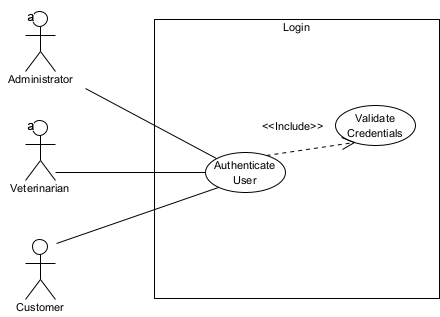
\includegraphics[width=\linewidth,keepaspectratio]{./media/CU01_Inicio_Sesion.png}
\end{center}

\protect\phantomsection\label{fig31}{}Ilustración 4. Caso de uso
Inicio de sesión

\begin{center}
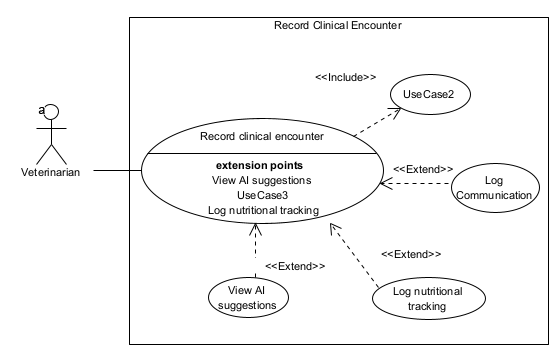
\includegraphics[width=\linewidth,keepaspectratio]{./media/CU02_Registrar_Atencion_Clinica.png}
\end{center}

\protect\phantomsection\label{fig32}{}Ilustración 5. Caso de uso
Registrar atención clínica

\begin{quote}
\begin{center}
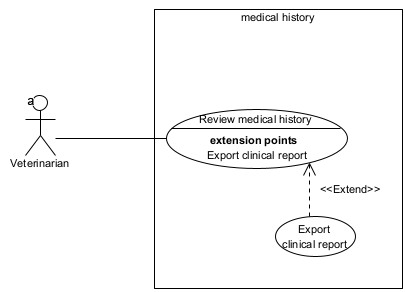
\includegraphics[width=\linewidth,keepaspectratio]{./media/CU03_Historial_Clinico.png}
\end{center}
\end{quote}

\protect\phantomsection\label{fig33}{}Ilustración 6. Caso de uso
Historial clínico

\begin{center}
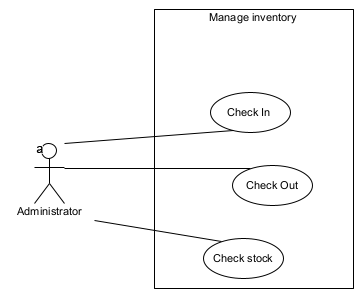
\includegraphics[width=\linewidth,keepaspectratio]{./media/CU04_Controlar_Inventario.png}
\end{center}

\protect\phantomsection\label{fig34}{}Ilustración 7. Caso de uso
Controlar inventario

\begin{quote}
\begin{center}
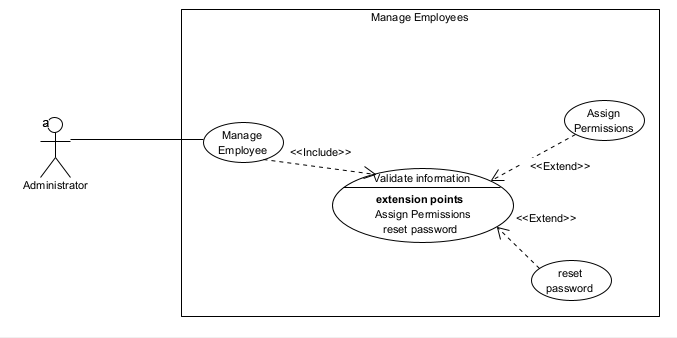
\includegraphics[width=\linewidth,keepaspectratio]{./media/CU05_Administrar_Empleados.png}
\end{center}
\end{quote}

\protect\phantomsection\label{fig35}{}Ilustración 8. Caso de uso
Administrar empleados

\begin{center}
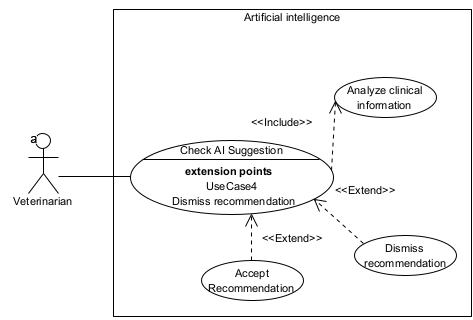
\includegraphics[width=\linewidth,keepaspectratio]{./media/CU06_Inteligencia_Artificial.png}
\end{center}

\begin{quote}
\protect\phantomsection\label{fig36}{}Ilustración 9. Caso de uso
Inteligencia Artificial

\begin{center}
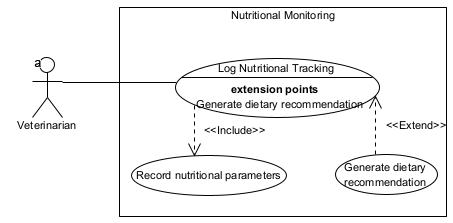
\includegraphics[width=\linewidth,keepaspectratio]{./media/CU07_Seguimiento_Nutricional.png}
\end{center}
\end{quote}

\protect\phantomsection\label{fig37}{}Ilustración 10. Caso de uso
Seguimiento nutricional

\begin{center}
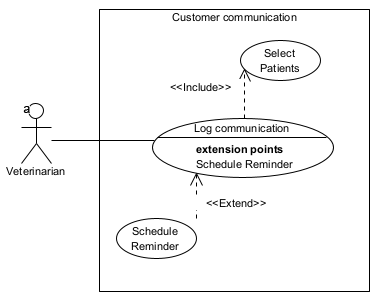
\includegraphics[width=\linewidth,keepaspectratio]{./media/CU08_Comunicacion _Cliente.png}
\end{center}

\protect\phantomsection\label{fig38}{}Ilustración 11. Caso de uso
Comunicación con cliente

\begin{center}
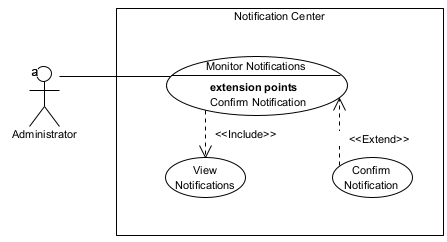
\includegraphics[width=\linewidth,keepaspectratio]{./media/CU09_Centro_Notificaciones.png}
\end{center}

\protect\phantomsection\label{fig39}{}Ilustración 12. Caso de uso
Centro de notificación

\begin{center}
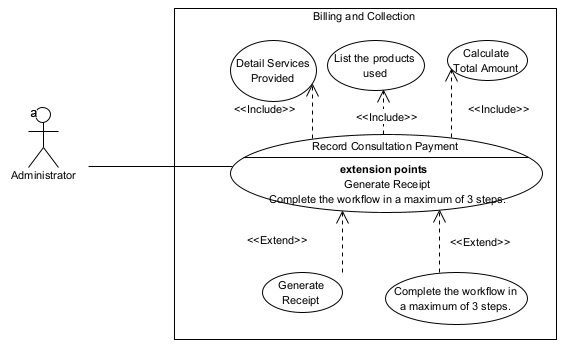
\includegraphics[width=\linewidth,keepaspectratio]{./media/CU10_Facturacion_Cobro.png}
\end{center}

\protect\phantomsection\label{fig39b}{}Ilustración 13. Caso de uso
Facturación y cobro

\subsection{4.2 Caso de uso general del
SGCV-IA}\label{caso-de-uso-general-del-sgcv-ia}

\begin{center}
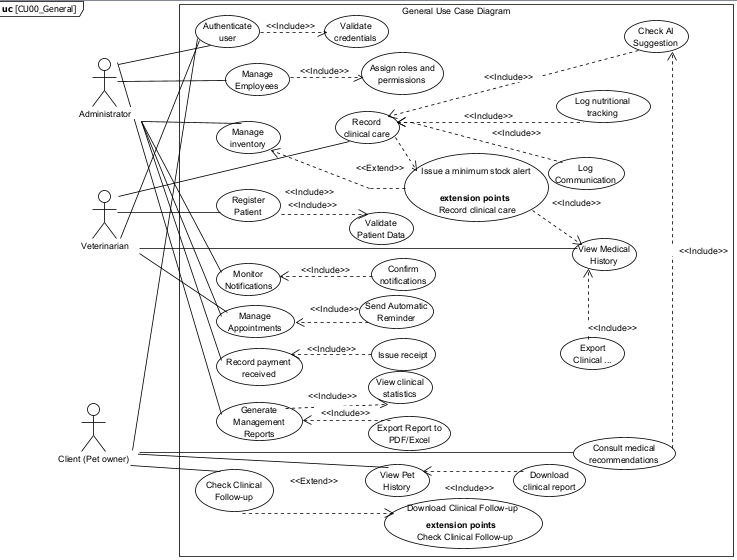
\includegraphics[width=\linewidth,keepaspectratio]{./media/CU00_General.png}
\end{center}

\begin{quote}
\protect\phantomsection\label{fig40}{}Ilustración 14. Caso de uso
general del SGCV-IA
\end{quote}

\subsection{4.3. Especificación de Casos de
Uso}\label{especificaciuxf3n-de-casos-de-uso}

{\def\LTcaptype{none} % do not increment counter
\begin{longtable}[]{@{}
  >{\raggedright\arraybackslash}p{(\linewidth - 2\tabcolsep) * \real{0.3188}}
  >{\raggedright\arraybackslash}p{(\linewidth - 2\tabcolsep) * \real{0.5504}}@{}}
\toprule\noalign{}
\begin{minipage}[b]{\linewidth}\raggedright
CU-01--- Iniciar Sesión
\end{minipage} & \begin{minipage}[b]{\linewidth}\raggedright
\textbf{Actor principal:} Administrador, Veterinario y Cliente \textbf{Actores secundarios:} Sistema de Autenticación
\textbf{Precondiciones:} El usuario debe estar registrado y su cuenta
debe encontrarse activa. \textbf{Postcondiciones (éxito):} El usuario accede al sistema con los
permisos correspondientes a su rol. \textbf{Flujo principal:}

\begin{enumerate}
\def\labelenumi{\arabic{enumi}.}
\item
  El usuario accede a la página de inicio de sesión.
\item
  Ingresa su usuario y contraseña.
\item
  El sistema valida las credenciales.
\item
  El sistema identifica el rol del usuario.
\item
  El sistema concede el acceso y muestra el panel correspondiente.
\end{enumerate}
\end{minipage} \\
\midrule\noalign{}
\endhead
\bottomrule\noalign{}
\endlastfoot
\end{longtable}
}

{\def\LTcaptype{none} % do not increment counter
\begin{longtable}[]{@{}
  >{\raggedright\arraybackslash}p{(\linewidth - 2\tabcolsep) * \real{0.3188}}
  >{\raggedright\arraybackslash}p{(\linewidth - 2\tabcolsep) * \real{0.5504}}@{}}
\toprule\noalign{}
\begin{minipage}[b]{\linewidth}\raggedright
\end{minipage} & \begin{minipage}[b]{\linewidth}\raggedright
\textbf{Flujos alternativos:} A1: Credenciales incorrectas → El sistema informa el error y permite un nuevo intento. A2: Campos obligatorios vacíos → El sistema solicita completar la
información. A3: Cuenta inactiva → El sistema deniega el acceso.
\textbf{Postcondición (fallo):} El usuario no accede al sistema.
\end{minipage} \\
\midrule\noalign{}
\endhead
\bottomrule\noalign{}
\endlastfoot
\end{longtable}
}

{\def\LTcaptype{none} % do not increment counter
\begin{longtable}[]{@{}
  >{\raggedright\arraybackslash}p{(\linewidth - 2\tabcolsep) * \real{0.3188}}
  >{\raggedright\arraybackslash}p{(\linewidth - 2\tabcolsep) * \real{0.5504}}@{}}
\toprule\noalign{}
\begin{minipage}[b]{\linewidth}\raggedright
\textbf{CU-02 --- Registrar Atención Clínica}
\end{minipage} & \begin{minipage}[b]{\linewidth}\raggedright
\textbf{Actor principal:} Veterinario \textbf{Actores secundarios:} Módulo de IA \textbf{Precondiciones:} El
veterinario ha iniciado sesión y el paciente se encuentra registrado. \textbf{Postcondiciones (éxito):} La atención clínica queda registrada y
el historial del paciente es actualizado. \textbf{Flujo principal:}

\begin{enumerate}
\def\labelenumi{\arabic{enumi}.}
\item
  El veterinario accede al módulo de atención clínica.
\item
  Selecciona al paciente.
\item
  El sistema muestra el historial clínico.
\item
  El veterinario registra el diagnóstico y tratamiento.
\item
  El sistema valida la información.
\item
  El sistema actualiza el historial clínico. \textbf{Flujos
  alternativos:} A1: El veterinario solicita sugerencias de IA → El
  sistema presenta recomendaciones para apoyar el diagnóstico.
\end{enumerate}

A2: El veterinario registra un seguimiento nutricional → El sistema almacena la información correspondiente. A3: El veterinario registra una comunicación con el dueño → El sistema
registra la comunicación en el historial. A4: Información incompleta → El sistema solicita corregir los datos
antes de guardar. \textbf{Postcondición (fallo):} La atención clínica no es registrada.
\end{minipage} \\
\midrule\noalign{}
\endhead
\bottomrule\noalign{}
\endlastfoot
\end{longtable}
}

{\def\LTcaptype{none} % do not increment counter
\begin{longtable}[]{@{}
  >{\raggedright\arraybackslash}p{(\linewidth - 2\tabcolsep) * \real{0.4347}}
  >{\raggedright\arraybackslash}p{(\linewidth - 2\tabcolsep) * \real{0.4345}}@{}}
\toprule\noalign{}
\begin{minipage}[b]{\linewidth}\raggedright
CU-03 --- Revisar Historial Clínico
\end{minipage} & \begin{minipage}[b]{\linewidth}\raggedright
\textbf{Actor principal:} Veterinario \textbf{Actores secundarios:} Ninguno \textbf{Precondiciones:} El
paciente debe estar registrado en el sistema. \textbf{Postcondiciones (éxito):} El historial clínico es consultado
correctamente.
\end{minipage} \\
\midrule\noalign{}
\endhead
\bottomrule\noalign{}
\endlastfoot
\end{longtable}
}

{\def\LTcaptype{none} % do not increment counter
\begin{longtable}[]{@{}
  >{\raggedright\arraybackslash}p{(\linewidth - 2\tabcolsep) * \real{0.4347}}
  >{\raggedright\arraybackslash}p{(\linewidth - 2\tabcolsep) * \real{0.4345}}@{}}
\toprule\noalign{}
\begin{minipage}[b]{\linewidth}\raggedright
\end{minipage} & \begin{minipage}[b]{\linewidth}\raggedright
\textbf{Flujo principal:}

\begin{enumerate}
\def\labelenumi{\arabic{enumi}.}
\item
  El veterinario accede al módulo de historial clínico.
\item
  Busca al paciente.
\item
  El sistema muestra el historial clínico.
\item
  El veterinario revisa la información médica registrada.
\end{enumerate}

\textbf{Flujos alternativos:} A1: El paciente no existe → El sistema informa que no se encontraron
registros. A2: El veterinario exporta el historial → El sistema genera
el reporte clínico. \textbf{Postcondición (fallo):} No se muestra información del historial.
\end{minipage} \\
\midrule\noalign{}
\endhead
\bottomrule\noalign{}
\endlastfoot
\end{longtable}
}

{\def\LTcaptype{none} % do not increment counter
\begin{longtable}[]{@{}
  >{\raggedright\arraybackslash}p{(\linewidth - 2\tabcolsep) * \real{0.4347}}
  >{\raggedright\arraybackslash}p{(\linewidth - 2\tabcolsep) * \real{0.4345}}@{}}
\toprule\noalign{}
\begin{minipage}[b]{\linewidth}\raggedright
CU-04 --- Controlar Inventario
\end{minipage} & \begin{minipage}[b]{\linewidth}\raggedright
\textbf{Actor principal:} Administrador \textbf{Actores secundarios:}
Sistema de Notificaciones \textbf{Precondiciones:} El administrador ha iniciado sesión. \textbf{Postcondiciones (éxito):} El inventario queda actualizado. \textbf{Flujo principal:}

\begin{enumerate}
\def\labelenumi{\arabic{enumi}.}
\item
  El administrador accede al módulo de inventario.
\item
  El sistema muestra los productos registrados.
\item
  El administrador registra una entrada o salida de productos.
\item
  El sistema actualiza el stock.
\item
  El sistema guarda los cambios realizados.
\end{enumerate}

\textbf{Flujos alternativos:} A1: Stock insuficiente → El sistema rechaza la operación. A2: Stock mínimo alcanzado → El sistema genera una alerta de
abastecimiento. Postcondición (fallo): El inventario permanece sin cambios.
\end{minipage} \\
\midrule\noalign{}
\endhead
\bottomrule\noalign{}
\endlastfoot
\end{longtable}
}

{\def\LTcaptype{none} % do not increment counter
\begin{longtable}[]{@{}
  >{\raggedright\arraybackslash}p{(\linewidth - 2\tabcolsep) * \real{0.4347}}
  >{\raggedright\arraybackslash}p{(\linewidth - 2\tabcolsep) * \real{0.4345}}@{}}
\toprule\noalign{}
\begin{minipage}[b]{\linewidth}\raggedright
CU-05 --- Gestionar Empleados
\end{minipage} & \begin{minipage}[b]{\linewidth}\raggedright
\textbf{Actor principal:} Administrador \textbf{Actores secundarios:}
Ninguno \textbf{Precondiciones:} El administrador ha iniciado sesión. \textbf{Postcondiciones (éxito):} La información del empleado queda
actualizada correctamente.
\end{minipage} \\
\midrule\noalign{}
\endhead
\bottomrule\noalign{}
\endlastfoot
\end{longtable}
}

{\def\LTcaptype{none} % do not increment counter
\begin{longtable}[]{@{}
  >{\raggedright\arraybackslash}p{(\linewidth - 2\tabcolsep) * \real{0.4347}}
  >{\raggedright\arraybackslash}p{(\linewidth - 2\tabcolsep) * \real{0.4345}}@{}}
\toprule\noalign{}
\begin{minipage}[b]{\linewidth}\raggedright
\end{minipage} & \begin{minipage}[b]{\linewidth}\raggedright
\textbf{Flujo principal}

\begin{enumerate}
\def\labelenumi{\arabic{enumi}.}
\item
  El administrador accede al módulo de gestión de personal.
\item
  Selecciona el empleado que desea administrar.
\item
  El sistema muestra la información del empleado.
\item
  El administrador realiza las modificaciones necesarias.
\item
  El sistema valida la información ingresada.
\item
  El sistema guarda los cambios realizados.
\end{enumerate}

\textbf{Flujos alternativos} A1: El administrador asigna permisos al empleado → El sistema actualiza
el rol y los permisos correspondientes. A2: El administrador restablece la contraseña del empleado → El sistema
genera una nueva contraseña o solicita definir una nueva. A3: Información inválida → El sistema informa los errores encontrados y
solicita corregirlos. \textbf{Postcondición (fallo):} Los cambios no son almacenados.
\end{minipage} \\
\midrule\noalign{}
\endhead
\bottomrule\noalign{}
\endlastfoot
\end{longtable}
}

{\def\LTcaptype{none} % do not increment counter
\begin{longtable}[]{@{}
  >{\raggedright\arraybackslash}p{(\linewidth - 2\tabcolsep) * \real{0.3188}}
  >{\raggedright\arraybackslash}p{(\linewidth - 2\tabcolsep) * \real{0.5504}}@{}}
\toprule\noalign{}
\begin{minipage}[b]{\linewidth}\raggedright
CU-06 --- Generar Sugerencia Diagnóstica con IA
\end{minipage} & \begin{minipage}[b]{\linewidth}\raggedright
\textbf{Actor principal:} Médico veterinario \textbf{Actores
secundarios:} Motor de Inteligencia Artificial (externo)
\textbf{Precondiciones:} El veterinario ha registrado los datos clínicos
de la consulta (RF-04). \textbf{Postcondiciones (éxito):} La sugerencia diagnóstica queda
registrada en el historial únicamente si fue aprobada, modificada o
formalmente rechazada por el veterinario.
\end{minipage} \\
\midrule\noalign{}
\endhead
\bottomrule\noalign{}
\endlastfoot
\end{longtable}
}

{\def\LTcaptype{none} % do not increment counter
\begin{longtable}[]{@{}
  >{\raggedright\arraybackslash}p{(\linewidth - 2\tabcolsep) * \real{0.4347}}
  >{\raggedright\arraybackslash}p{(\linewidth - 2\tabcolsep) * \real{0.4345}}@{}}
\toprule\noalign{}
\begin{minipage}[b]{\linewidth}\raggedright
\end{minipage} & \begin{minipage}[b]{\linewidth}\raggedright
\textbf{Flujo principal}

\begin{enumerate}
\def\labelenumi{\arabic{enumi}.}
\item
  El veterinario solicita al sistema una sugerencia diagnóstica sobre la
  consulta activa.
\item
  El sistema envía los datos clínicos anonimizados al motor de IA
  externo.
\item
  El motor de IA retorna posibles diagnósticos diferenciales con
  referencia bibliográfica y nivel de confianza (RNF-09, RNF-16).
\item
  El sistema muestra al veterinario la sugerencia, los factores
  considerados y el nivel de confianza.
\item
  El veterinario acepta, modifica o rechaza la sugerencia.
\item
  El sistema registra la decisión y, si corresponde, incorpora la
  sugerencia validada al historial clínico.
\end{enumerate}

\textbf{Flujos alternativos} A1: El servicio de IA no responde → El sistema notifica la
indisponibilidad y permite continuar la consulta sin sugerencia
(RNF-10). A2: El veterinario rechaza la sugerencia → El sistema registra el
rechazo sin incorporar la sugerencia al historial. \textbf{Postcondición (fallo):} Ninguna sugerencia queda registrada sin
una acción explícita del veterinario.
\end{minipage} \\
\midrule\noalign{}
\endhead
\bottomrule\noalign{}
\endlastfoot
\end{longtable}
}

{\def\LTcaptype{none} % do not increment counter
\begin{longtable}[]{@{}
  >{\raggedright\arraybackslash}p{(\linewidth - 2\tabcolsep) * \real{0.3188}}
  >{\raggedright\arraybackslash}p{(\linewidth - 2\tabcolsep) * \real{0.5504}}@{}}
\toprule\noalign{}
\begin{minipage}[b]{\linewidth}\raggedright
CU-07 --- Gestionar Facturación y Cobro
\end{minipage} & \begin{minipage}[b]{\linewidth}\raggedright
\textbf{Actor principal:} Personal administrativo \textbf{Actores
secundarios:} Ninguno \textbf{Precondiciones:} La consulta o los
servicios/productos a cobrar están registrados. \textbf{Postcondiciones (éxito):} Se emite un comprobante asociado al
cobro registrado.
\end{minipage} \\
\midrule\noalign{}
\endhead
\bottomrule\noalign{}
\endlastfoot
\end{longtable}
}

{\def\LTcaptype{none} % do not increment counter
\begin{longtable}[]{@{}
  >{\raggedright\arraybackslash}p{(\linewidth - 2\tabcolsep) * \real{0.4347}}
  >{\raggedright\arraybackslash}p{(\linewidth - 2\tabcolsep) * \real{0.4345}}@{}}
\toprule\noalign{}
\begin{minipage}[b]{\linewidth}\raggedright
\end{minipage} & \begin{minipage}[b]{\linewidth}\raggedright
\textbf{Flujo principal}

\begin{enumerate}
\def\labelenumi{\arabic{enumi}.}
\item
  El personal administrativo selecciona la consulta a facturar.
\item
  El sistema calcula automáticamente el monto total (servicios y
  productos utilizados).
\item
  El personal confirma el cobro.
\item
  El sistema genera el comprobante en un máximo de 3 pasos (RF-08,
  RNF-02).
\end{enumerate}

\textbf{Flujos alternativos} A1: Monto incorrecto → El personal ajusta manualmente los ítems antes de
confirmar. \textbf{Postcondición (fallo):} No se emite comprobante y la consulta
queda pendiente de cobro.
\end{minipage} \\
\midrule\noalign{}
\endhead
\bottomrule\noalign{}
\endlastfoot
\end{longtable}
}

{\def\LTcaptype{none} % do not increment counter
\begin{longtable}[]{@{}
  >{\raggedright\arraybackslash}p{(\linewidth - 2\tabcolsep) * \real{0.3188}}
  >{\raggedright\arraybackslash}p{(\linewidth - 2\tabcolsep) * \real{0.5504}}@{}}
\toprule\noalign{}
\begin{minipage}[b]{\linewidth}\raggedright
CU-08 --- Registrar Seguimiento Nutricional
\end{minipage} & \begin{minipage}[b]{\linewidth}\raggedright
\textbf{Actor principal:} Médico veterinario \textbf{Actores
secundarios:} Ninguno \textbf{Precondiciones:} El paciente cuenta con al
menos un registro previo de peso o condición corporal. \textbf{Postcondiciones (éxito):} El nuevo dato se incorpora al
historial de seguimiento y la recomendación nutricional se actualiza.
\end{minipage} \\
\midrule\noalign{}
\endhead
\bottomrule\noalign{}
\endlastfoot
\end{longtable}
}

{\def\LTcaptype{none} % do not increment counter
\begin{longtable}[]{@{}
  >{\raggedright\arraybackslash}p{(\linewidth - 2\tabcolsep) * \real{0.4347}}
  >{\raggedright\arraybackslash}p{(\linewidth - 2\tabcolsep) * \real{0.4345}}@{}}
\toprule\noalign{}
\begin{minipage}[b]{\linewidth}\raggedright
\end{minipage} & \begin{minipage}[b]{\linewidth}\raggedright
\textbf{Flujo principal}

\begin{enumerate}
\def\labelenumi{\arabic{enumi}.}
\item
  El veterinario registra el peso, la edad y la condición corporal
  actual del paciente (RF-13).
\item
  El sistema actualiza el gráfico de tendencia de peso.
\item
  El sistema genera automáticamente una recomendación nutricional
  personalizada (RF-14).
\item
  El veterinario revisa y comunica la recomendación al propietario.
\end{enumerate}

\textbf{Flujos alternativos} A1: Datos insuficientes para generar recomendación → El sistema solicita
completar raza, edad o peso antes de continuar. \textbf{Postcondición (fallo):} El registro de seguimiento no se guarda.
\end{minipage} \\
\midrule\noalign{}
\endhead
\bottomrule\noalign{}
\endlastfoot
\end{longtable}
}

{\def\LTcaptype{none} % do not increment counter
\begin{longtable}[]{@{}
  >{\raggedright\arraybackslash}p{(\linewidth - 2\tabcolsep) * \real{0.3188}}
  >{\raggedright\arraybackslash}p{(\linewidth - 2\tabcolsep) * \real{0.5504}}@{}}
\toprule\noalign{}
\begin{minipage}[b]{\linewidth}\raggedright
CU-09 --- Enviar Comunicación y Notificaciones al Cliente
\end{minipage} & \begin{minipage}[b]{\linewidth}\raggedright
\textbf{Actor principal:} Personal administrativo / médico veterinario
\textbf{Actores secundarios:} Servicio de mensajería (WhatsApp, externo)
\textbf{Precondiciones:} El paciente tiene un propietario con datos de
contacto registrados. \textbf{Postcondiciones (éxito):} La comunicación queda registrada en el
historial del paciente con fecha y resumen.
\end{minipage} \\
\midrule\noalign{}
\endhead
\bottomrule\noalign{}
\endlastfoot
\end{longtable}
}

{\def\LTcaptype{none} % do not increment counter
\begin{longtable}[]{@{}
  >{\raggedright\arraybackslash}p{(\linewidth - 2\tabcolsep) * \real{0.4347}}
  >{\raggedright\arraybackslash}p{(\linewidth - 2\tabcolsep) * \real{0.4345}}@{}}
\toprule\noalign{}
\begin{minipage}[b]{\linewidth}\raggedright
\end{minipage} & \begin{minipage}[b]{\linewidth}\raggedright
\textbf{Flujo principal}

\begin{enumerate}
\def\labelenumi{\arabic{enumi}.}
\item
  El usuario selecciona el paciente y el tipo de comunicación (resultado
  de examen, recordatorio, indicación médica) (RF-09, RF-10, RF-12,
  RF-15).
\item
  El sistema adjunta el archivo o mensaje correspondiente.
\item
  El sistema envía la comunicación por WhatsApp.
\item
  El sistema registra fecha, tipo y resumen en la ficha del paciente.
\end{enumerate}

\textbf{Flujos alternativos} A1: Falla el servicio de mensajería externo → El sistema notifica el
error y permite reintentar el envío. \textbf{Postcondición (fallo):} La comunicación no queda registrada como
enviada.
\end{minipage} \\
\midrule\noalign{}
\endhead
\bottomrule\noalign{}
\endlastfoot
\end{longtable}
}

{\def\LTcaptype{none} % do not increment counter
\begin{longtable}[]{@{}
  >{\raggedright\arraybackslash}p{(\linewidth - 2\tabcolsep) * \real{0.3188}}
  >{\raggedright\arraybackslash}p{(\linewidth - 2\tabcolsep) * \real{0.5504}}@{}}
\toprule\noalign{}
\begin{minipage}[b]{\linewidth}\raggedright
CU-10 --- Consultar Centro de Notificaciones y Alertas de Inventario
\end{minipage} & \begin{minipage}[b]{\linewidth}\raggedright
\textbf{Actor principal:} Personal administrativo / Bodeguero
\textbf{Actores secundarios:} Ninguno \textbf{Precondiciones:} El
usuario ha iniciado sesión con un perfil autorizado. \textbf{Postcondiciones (éxito):} El usuario visualiza las alertas
activas (vencimiento de productos, stock mínimo) y puede marcarlas como
atendidas.
\end{minipage} \\
\midrule\noalign{}
\endhead
\bottomrule\noalign{}
\endlastfoot
\end{longtable}
}

{\def\LTcaptype{none} % do not increment counter
\begin{longtable}[]{@{}
  >{\raggedright\arraybackslash}p{(\linewidth - 2\tabcolsep) * \real{0.4347}}
  >{\raggedright\arraybackslash}p{(\linewidth - 2\tabcolsep) * \real{0.4345}}@{}}
\toprule\noalign{}
\begin{minipage}[b]{\linewidth}\raggedright
\end{minipage} & \begin{minipage}[b]{\linewidth}\raggedright
\textbf{Flujo principal}

\begin{enumerate}
\def\labelenumi{\arabic{enumi}.}
\item
  El sistema genera alertas automáticas cuando un producto se aproxima a
  su fecha de vencimiento (30, 15 o 7 días) o el stock cae bajo el
  umbral configurado (RF-05, RF-06).
\item
  El usuario accede al centro de notificaciones.
\item
  El sistema lista las alertas activas ordenadas por urgencia.
\item
  El usuario marca una alerta como atendida.
\end{enumerate}

\textbf{Flujos alternativos} A1: No hay alertas activas → El sistema muestra el centro de
notificaciones vacío. \textbf{Postcondición (fallo):} La alerta permanece activa si no es
marcada como atendida.
\end{minipage} \\
\midrule\noalign{}
\endhead
\bottomrule\noalign{}
\endlastfoot
\end{longtable}
}

\begin{quote}
Resumen: se documentaron 10 casos de uso detallados (CU-01 a CU-10),
cubriendo la totalidad de los módulos representados en el diagrama de
casos de uso general (Sección 4.1).
\end{quote}

\subsection{4.4. Diagrama de Clases
Conceptual}\label{diagrama-de-clases-conceptual}

{\def\LTcaptype{none} % do not increment counter
\begin{longtable}[]{@{}
  >{\raggedright\arraybackslash}p{(\linewidth - 4\tabcolsep) * \real{0.3191}}
  >{\raggedright\arraybackslash}p{(\linewidth - 4\tabcolsep) * \real{0.1536}}
  >{\raggedright\arraybackslash}p{(\linewidth - 4\tabcolsep) * \real{0.4058}}@{}}
\toprule\noalign{}
\multicolumn{3}{@{}>{\centering\arraybackslash}p{(\linewidth - 4\tabcolsep) * \real{0.8785} + 4\tabcolsep}@{}}{%
\begin{minipage}[b]{\linewidth}\centering
\textbf{Relaciones Principales y Multiplicidad}
\end{minipage}} \\
\midrule\noalign{}
\endhead
\bottomrule\noalign{}
\endlastfoot
\textbf{Relación} & \textbf{Multiplicidad} & \textbf{Justificación} \\
Usuario - Administrador & No aplica & Un administrador es un tipo de
usuario, por lo que hereda sus atributos y características generales. \\
Usuario --- Veterinario & No aplica & Un veterinario es un tipo de
usuario, compartiendo la información común definida en la clase
Usuario. \\
Cliente --- Paciente & 1: N & Un cliente puede ser propietario de varias
mascotas, mientras que cada paciente pertenece a un único cliente. \\
Paciente --- Historial & 1: 1 & Cada paciente posee un único historial

clínico, el cual no puede existir sin el paciente. \\
Paciente --- Atención Clínica & 1: N & Un paciente puede recibir
múltiples atenciones clínicas a lo largo del tiempo, pero cada atención
corresponde a un único paciente. \\
Historial Clínico --- Atención Clínica & 1: N & Un historial clínico
almacena todas las atenciones realizadas al paciente y estas no tienen
sentido sin el historial al que pertenecen. \\
\end{longtable}
}

{\def\LTcaptype{none} % do not increment counter
\begin{longtable}[]{@{}
  >{\raggedright\arraybackslash}p{(\linewidth - 4\tabcolsep) * \real{0.3191}}
  >{\raggedright\arraybackslash}p{(\linewidth - 4\tabcolsep) * \real{0.1536}}
  >{\raggedright\arraybackslash}p{(\linewidth - 4\tabcolsep) * \real{0.4058}}@{}}
\toprule\noalign{}
\begin{minipage}[b]{\linewidth}\raggedright
Veterinario --- Atención Clínica
\end{minipage} & \begin{minipage}[b]{\linewidth}\raggedright
1: N
\end{minipage} & \begin{minipage}[b]{\linewidth}\raggedright
Un veterinario puede realizar numerosas atenciones clínicas, mientras
que cada atención es realizada por un único veterinario
\end{minipage} \\
\midrule\noalign{}
\endhead
\bottomrule\noalign{}
\endlastfoot
Administrador --- Inventario & 1: 1 & El administrador supervisa el
inventario del sistema, siendo responsable de su gestión y actualización. \\
Inventario --- Producto & 1: N & Un inventario administra múltiples
productos. Los productos pueden existir independientemente del
inventario, por lo que no existe dependencia de vida. \\
Inventario --- Notificación & 1: N & El inventario puede generar
múltiples notificaciones relacionadas con bajo stock o vencimiento de productos, dependiendo de su estado. \\
\end{longtable}
}

\protect\phantomsection\label{table11}{}Tabla 11. Relaciones
principales y multiplicidad del diagrama de clases

\subsection{4.5. Diagramas de actividad}

\begin{figure}[H]
    \centering
    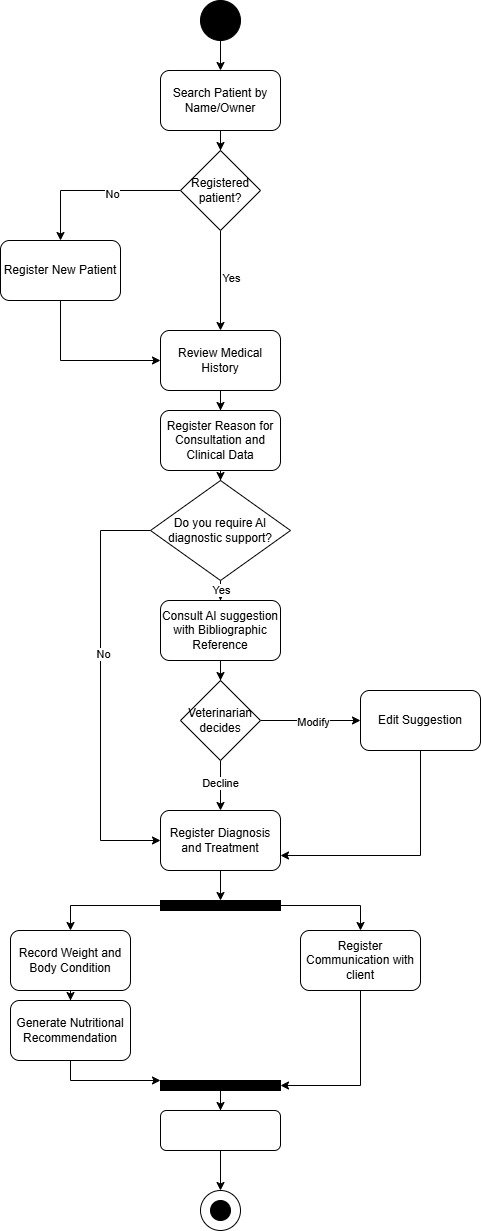
\includegraphics[height=0.65\textheight,keepaspectratio]{./media/DA01_Atencion_Clinica.png}
    \caption{Diagrama de actividad de atención clínica}
    \label{fig:da01}
\end{figure}

\protect\phantomsection\label{fig41}{}Ilustración 15. Diagrama de actividad de atención clínica

\begin{center}
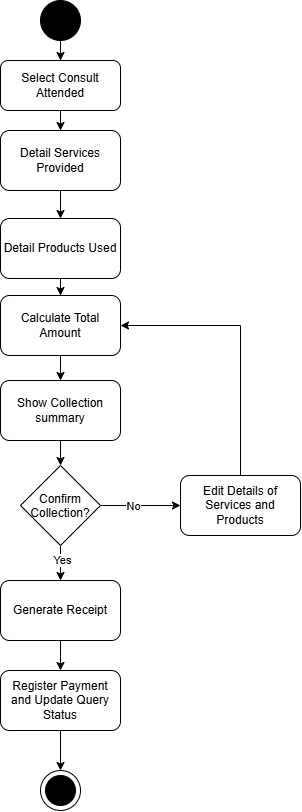
\includegraphics[height=0.55\textheight,keepaspectratio]{./media/DA02_Facturacion_Cobro.png}
\end{center}

\protect\phantomsection\label{fig42}{}Ilustración 16. Diagrama de actividad de facturación y cobro

\subsection{4.6. Diagrama de clase}\label{diagrama-de-clase}

\begin{center}
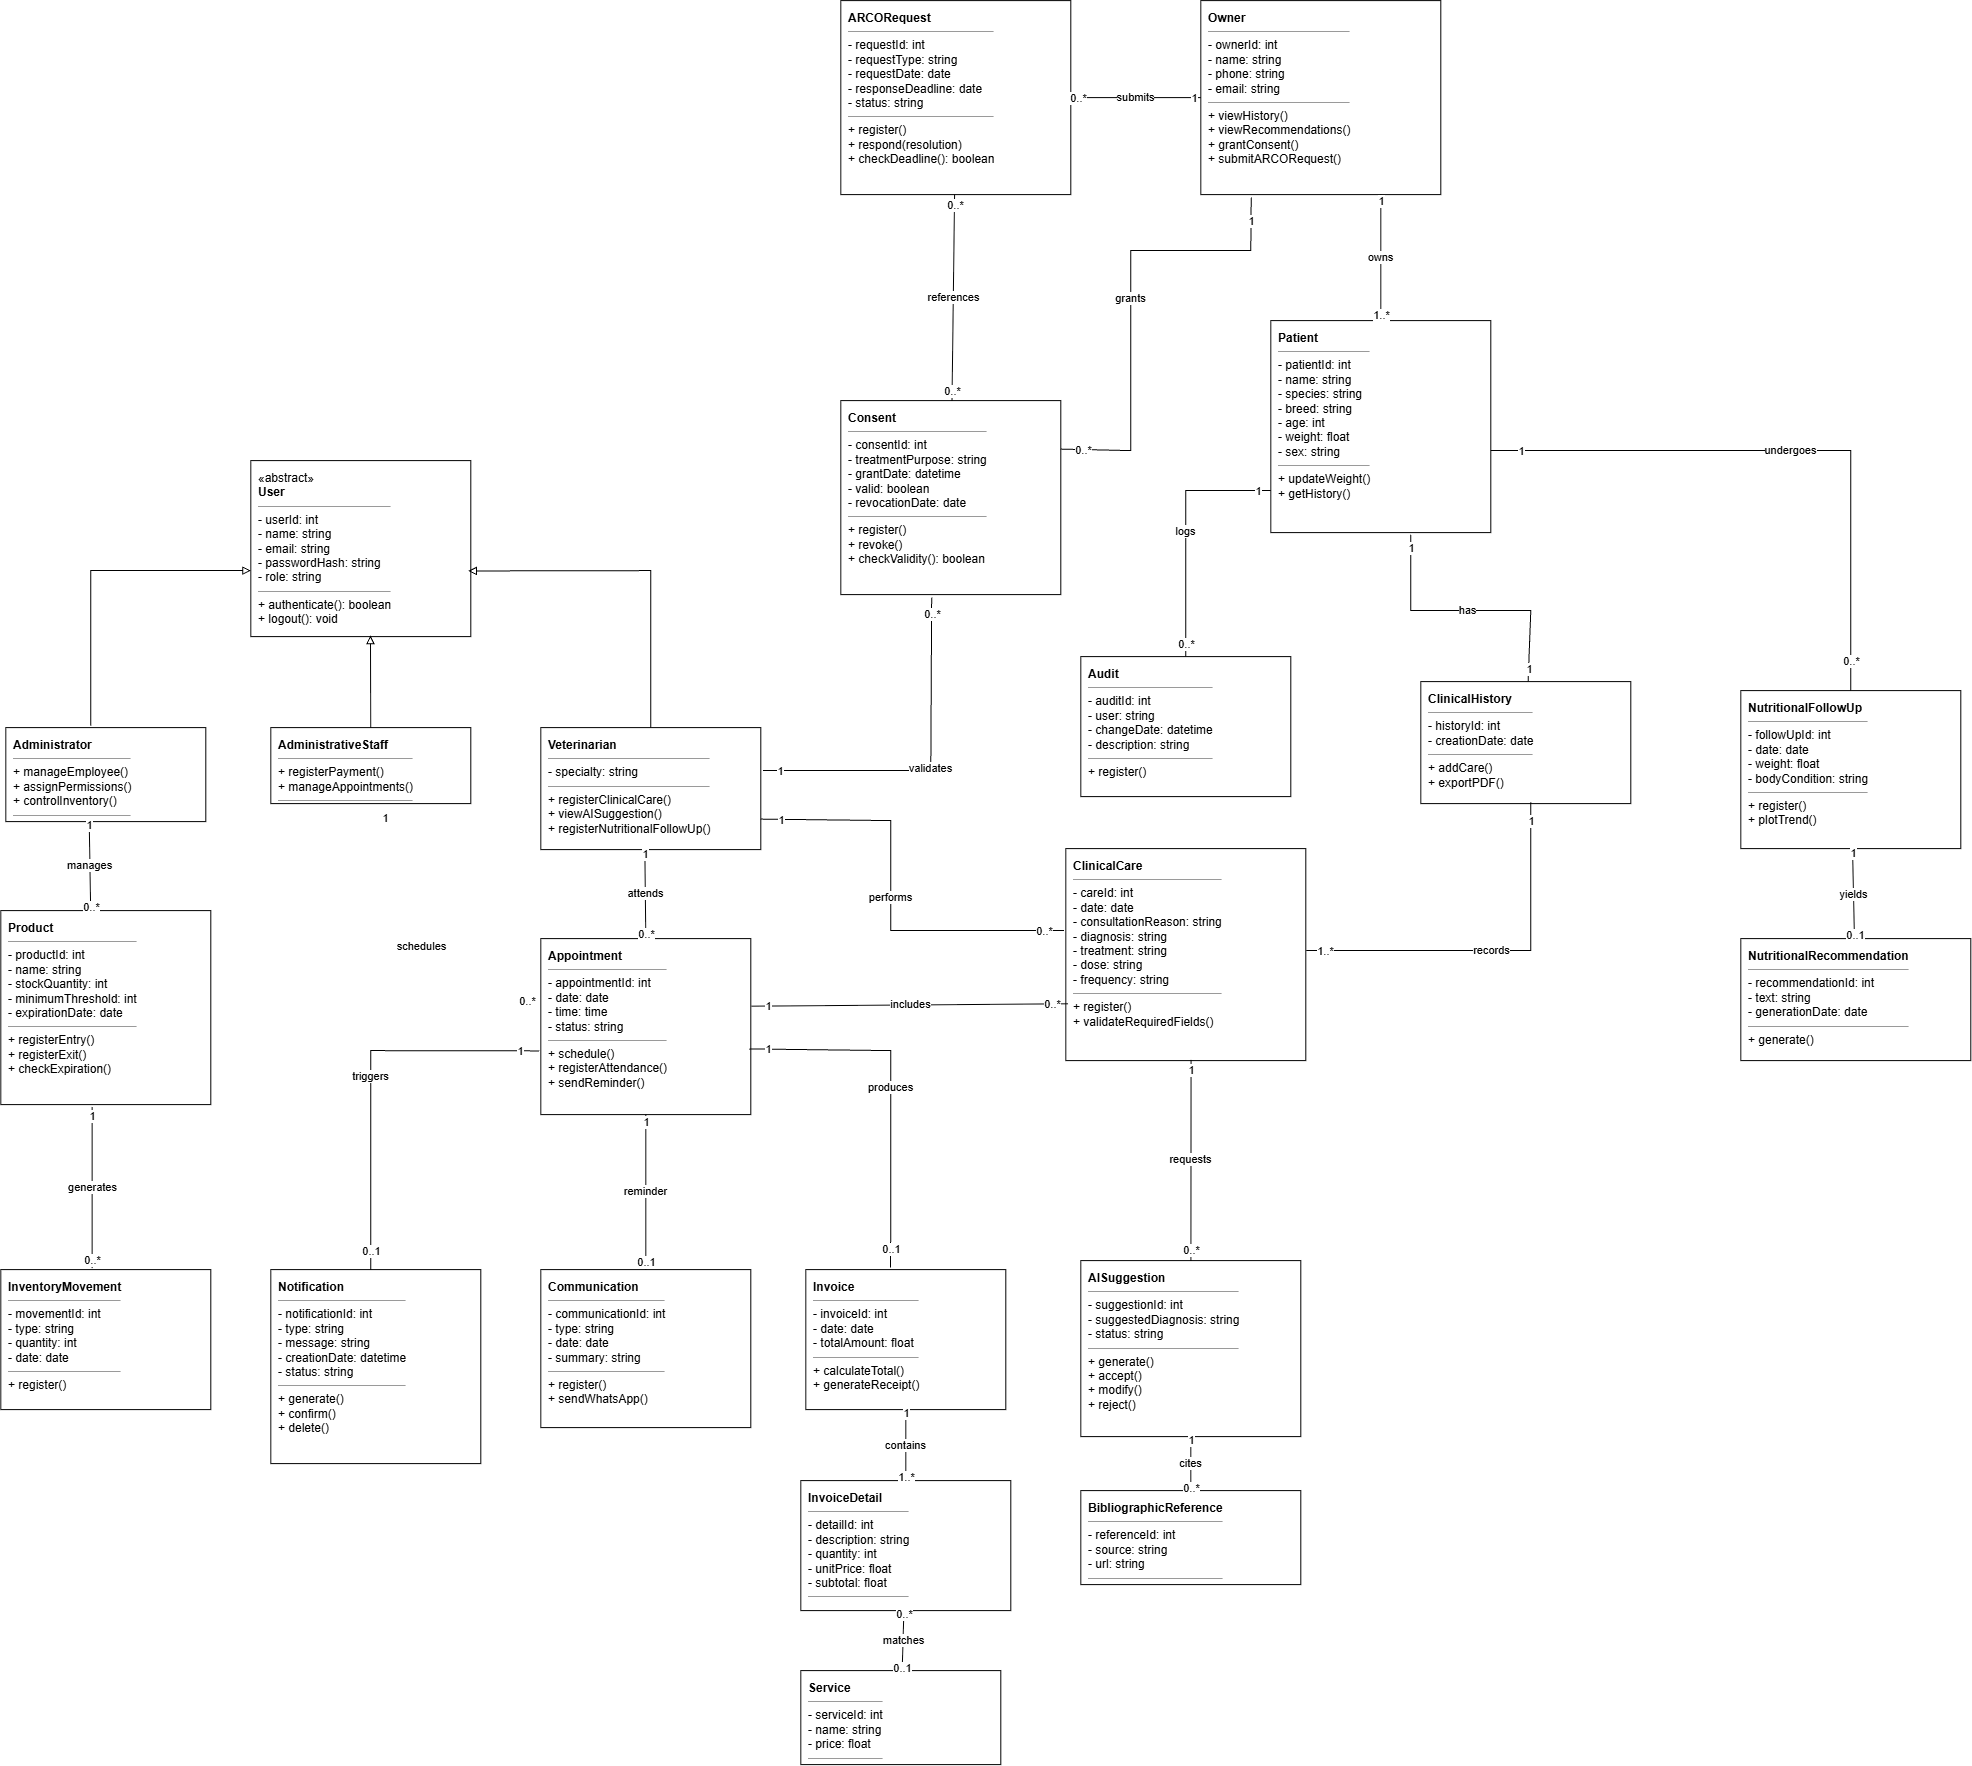
\includegraphics[width=\linewidth,keepaspectratio]{./media/DIAGRAMA_DE_CLASES_REFINADO_v3_1.png}
\end{center}

\protect\phantomsection\label{fig43}{}Ilustración 17. Diagrama de clases refinados

\subsection{4.7 Diagrama de componentes}

\begin{center}
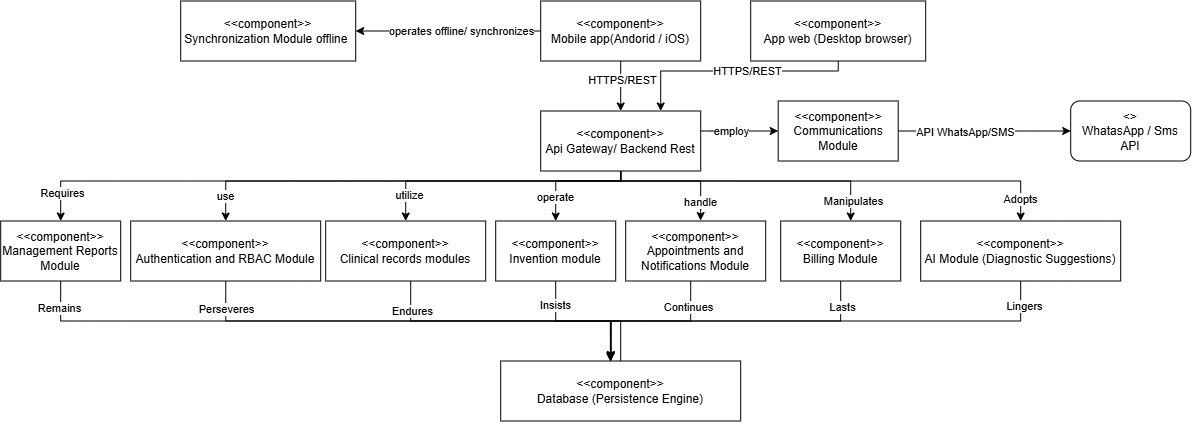
\includegraphics[width=\linewidth,keepaspectratio]{./media/Diagrama_De_Componente.png}
\end{center}

\protect\phantomsection\label{fig44}{}Ilustración 18. Diagrama de componentes

\textbf{4.8 Diagrama de despliegue}

\begin{center}
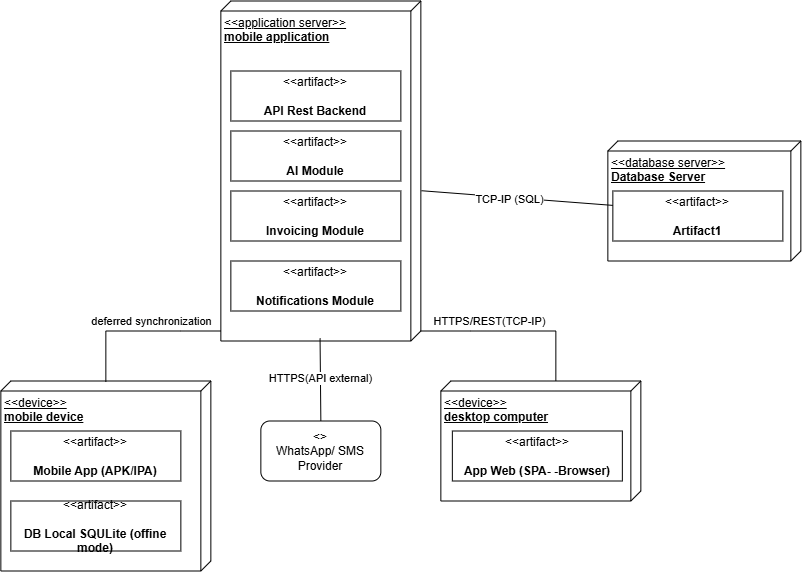
\includegraphics[width=\linewidth,keepaspectratio]{./media/Diagrama_De_Despligue.png}
\end{center}

\protect\phantomsection\label{fig45}{}Ilustración 19. Diagrama de despliegue

\textbf{4.9 Diagrama de estados}

\begin{center}
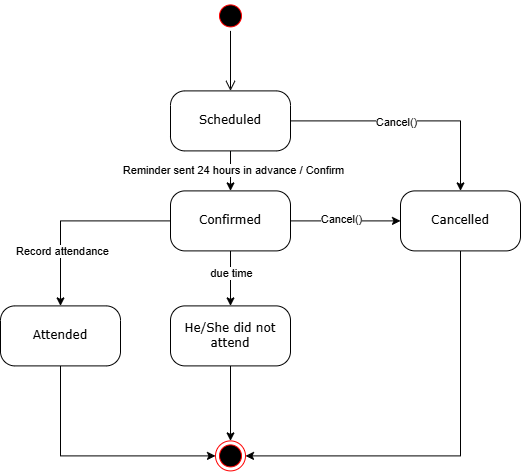
\includegraphics[width=\linewidth,keepaspectratio]{./media/Diagrama_De_Estados_Cita_Medica.png}
\end{center}

\protect\phantomsection\label{fig46}{}Ilustración 20. Diagrama de estados de cita médica

\begin{center}
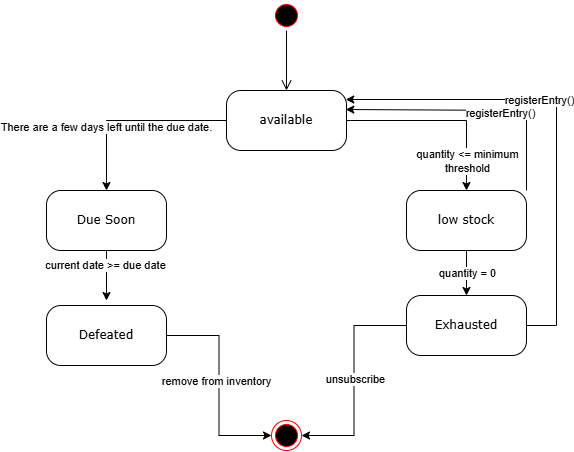
\includegraphics[width=\linewidth,keepaspectratio]{./media/Diagrama_De_Estados_Productos.png}
\end{center}

\protect\phantomsection\label{fig47}{}Ilustración 21. Diagrama de estados de productos

\textbf{4.10 Diagramas de secuencia}

\begin{center}
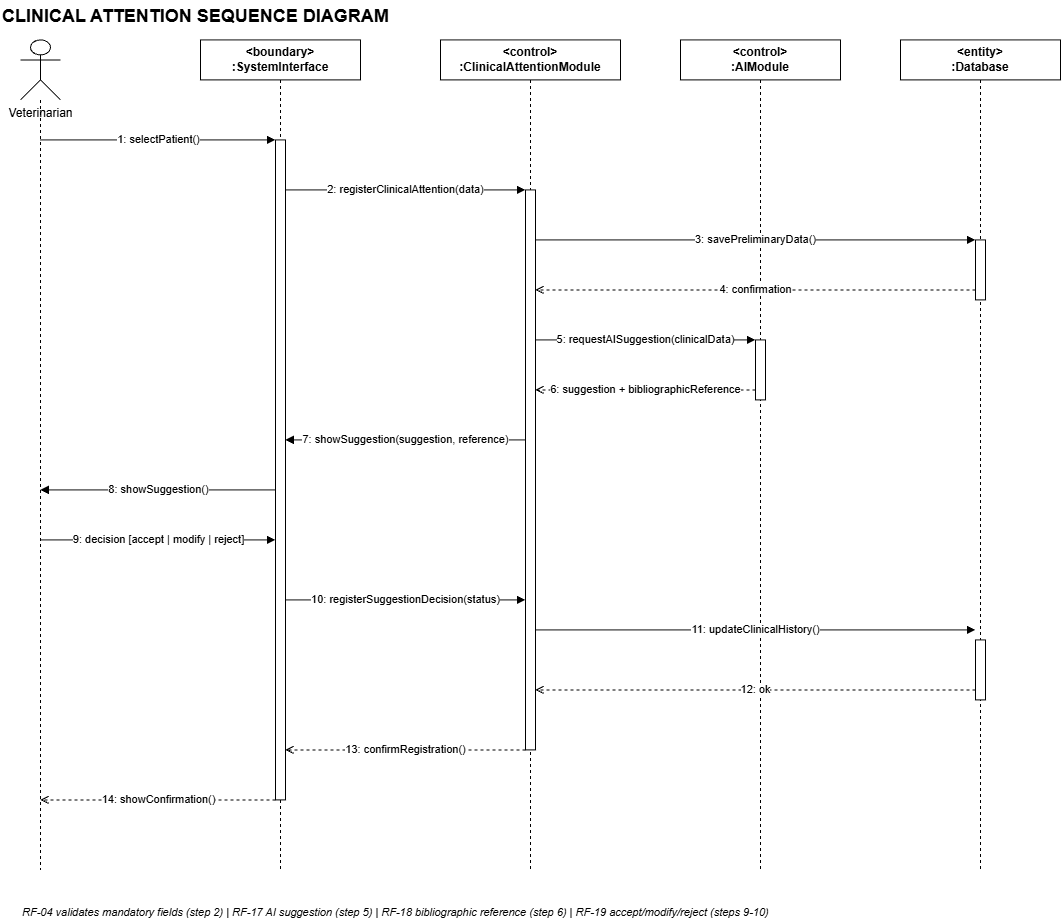
\includegraphics[width=\linewidth,keepaspectratio]{./media/DIAGRAMA_SECUANCIA_ATENCION_CLINICA.png}
\end{center}

\protect\phantomsection\label{fig48}{}Ilustración 22. Diagrama de secuencia de atención clínica

\begin{center}
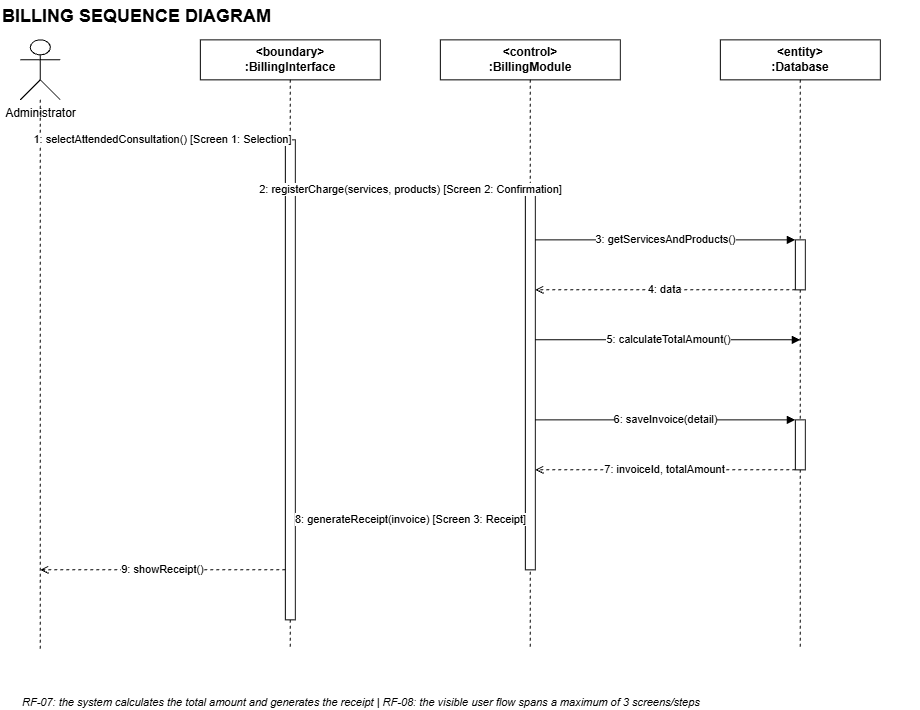
\includegraphics[width=\linewidth,keepaspectratio]{./media/DIAGRAMA_SECUENCIA_FACTURACION.png}
\end{center}

\protect\phantomsection\label{fig49}{}Ilustración 23. Diagrama de secuencia de facturación

\begin{center}
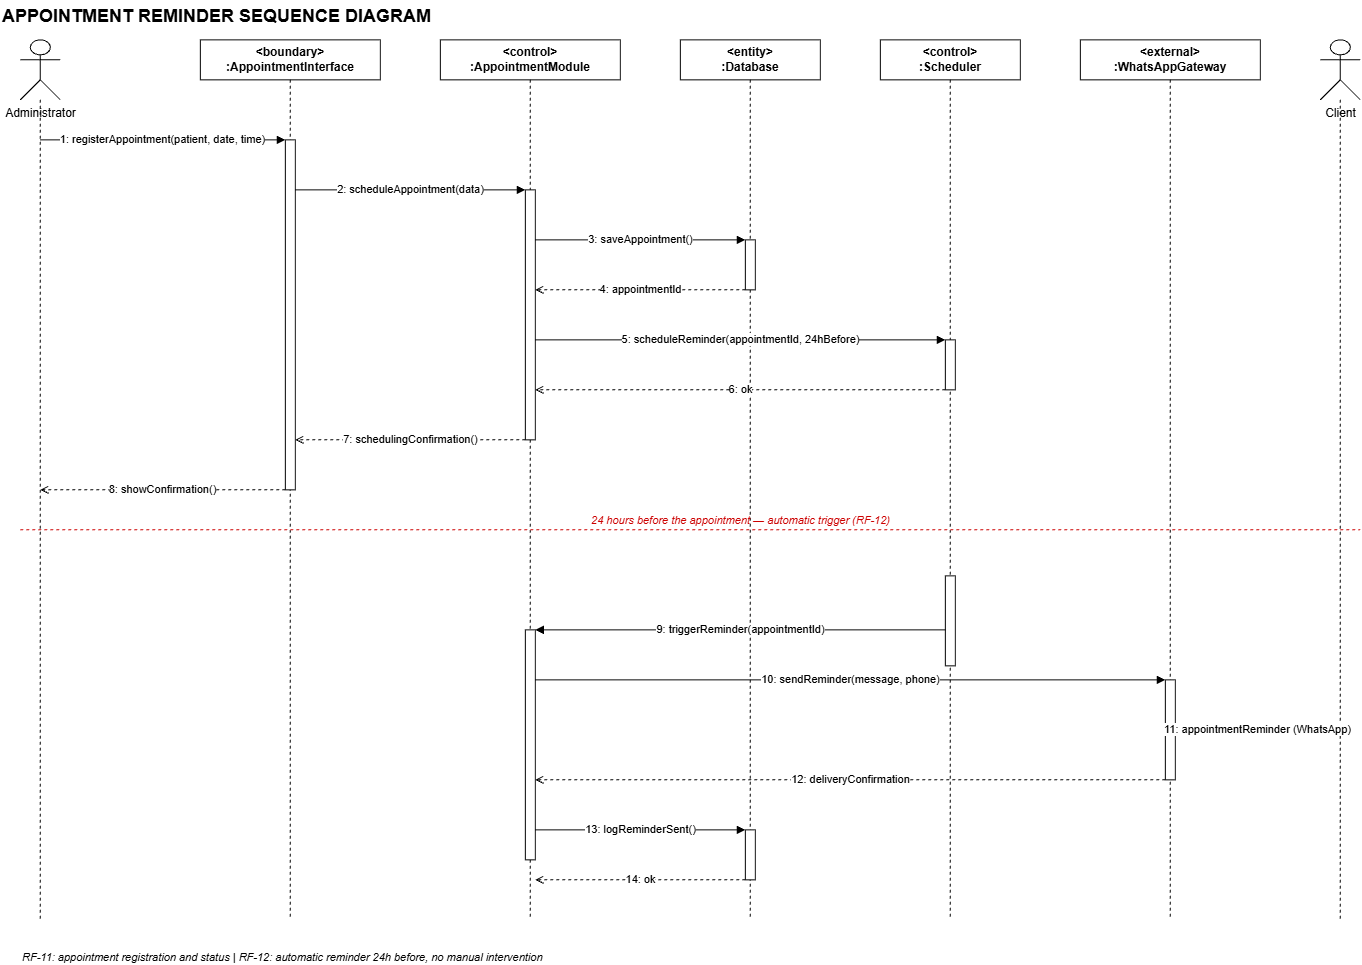
\includegraphics[width=\linewidth,keepaspectratio]{./media/DIAGRAMA_SECUENCIA_RECORDATORIO.png}
\end{center}

\protect\phantomsection\label{fig50}{}Ilustración 24. Diagrama de secuencia de recordatorio

\section{5. Priorización y
Trazabilidad}\label{priorizaciuxf3n-y-trazabilidad}

\begin{quote}
Clasificar todos los requisitos (RF/NFR/restricción), priorizarlos con
\textbf{MoSCoW} (justificando Must y Won\textquotesingle t) y construir
la \textbf{matriz de trazabilidad parcial} que enlace evidencia de campo
→ requisito → caso de uso.
\end{quote}

\begin{enumerate}
\def\labelenumi{\arabic{enumi}.}
\item
  \protect\phantomsection\label{_bookmark59}{}\textbf{Clasificación de
  Requisitos}
\end{enumerate}

\subsection{5.1. Clasificación de
requisitos}\label{clasificaciuxf3n-de-requisitos}

\paragraph{}\label{section-10}

\begin{quote}
Se clasifican los cuatro tipos de artefactos de requisitos identificados
en el documento: 25 Requisitos Funcionales (RF), 16 Requisitos No
Funcionales (RNF), 9 Restricciones (RST) y 14 Requisitos Legales (RL),
para un total de 64 elementos clasificados.
\end{quote}

{\def\LTcaptype{none} % do not increment counter
\begin{longtable}[]{@{}
  >{\centering\arraybackslash}p{(\linewidth - 4\tabcolsep) * \real{0.3604}}
  >{\centering\arraybackslash}p{(\linewidth - 4\tabcolsep) * \real{0.2775}}
  >{\centering\arraybackslash}p{(\linewidth - 4\tabcolsep) * \real{0.3184}}@{}}
\toprule\noalign{}
\begin{minipage}[b]{\linewidth}\centering
\textbf{Tipo}
\end{minipage} & \begin{minipage}[b]{\linewidth}\centering
\textbf{Cantidad}
\end{minipage} & \begin{minipage}[b]{\linewidth}\centering
\textbf{Rango de IDs}
\end{minipage} \\
\midrule\noalign{}
\endhead
\bottomrule\noalign{}
\endlastfoot
Requisito Funcional (RF) & 25 & RF-01 a RF-24, RF-26 (RF-25 reservado,
PE4) \\
Requisito No Funcional (RNF) & 16 & RNF-01 a RNF-16 \\
Restricción (RST) & 9 & RST-01 a RST-09 \\
Requisito Legal (RL) & 14 & RL-01 a RL-14 \\
\end{longtable}
}

\begin{quote}
\protect\phantomsection\label{table12}{}Tabla 12. Clasificación de
requisitos.
\end{quote}

{\def\LTcaptype{none} % do not increment counter
\begin{longtable}[]{@{}
  >{\raggedright\arraybackslash}p{(\linewidth - 4\tabcolsep) * \real{0.1157}}
  >{\raggedright\arraybackslash}p{(\linewidth - 4\tabcolsep) * \real{0.6334}}
  >{\raggedright\arraybackslash}p{(\linewidth - 4\tabcolsep) * \real{0.2070}}@{}}
\toprule\noalign{}
\begin{minipage}[b]{\linewidth}\centering
\textbf{ID}
\end{minipage} & \begin{minipage}[b]{\linewidth}\centering
\textbf{Restricción}
\end{minipage} & \begin{minipage}[b]{\linewidth}\raggedright
\textbf{Origen}
\end{minipage} \\
\midrule\noalign{}
\endhead
\bottomrule\noalign{}
\endlastfoot
RST-01 & \begin{minipage}[t]{\linewidth}\raggedright
Base de datos relacional (PostgreSQL/MySQL), sin NoSQL como
almacenamiento principal.
\end{minipage} & \begin{minipage}[t]{\linewidth}\raggedright
Sección 2.5 / 3.4
\end{minipage} \\
RST-02 & \begin{minipage}[t]{\linewidth}\raggedright
Cumplimiento de la normativa ecuatoriana de protección de datos
personales (LOPDP).
\end{minipage} & \begin{minipage}[t]{\linewidth}\raggedright
Sección 2.6
\end{minipage} \\
RST-03 & \begin{minipage}[t]{\linewidth}\raggedright
Autenticación y RBAC obligatorios por confidencialidad de datos
clínicos.
\end{minipage} & \begin{minipage}[t]{\linewidth}\raggedright
Sección 2.6
\end{minipage} \\
RST-04 & \begin{minipage}[t]{\linewidth}\raggedright
Uso prioritario de frameworks y bibliotecas de código abierto
(presupuesto).
\end{minipage} & \begin{minipage}[t]{\linewidth}\raggedright
Sección 2.6
\end{minipage} \\
RST-05 & \begin{minipage}[t]{\linewidth}\raggedright
Arquitectura cliente-servidor con API REST; módulo de IA desacoplado del
backend.
\end{minipage} & \begin{minipage}[t]{\linewidth}\raggedright
Sección 3.4
\end{minipage} \\
RST-06 & \begin{minipage}[t]{\linewidth}\raggedright
Sincronización offline mediante cola local de operaciones (no réplica
completa de base de datos en cliente).
\end{minipage} & \begin{minipage}[t]{\linewidth}\raggedright
Sección 3.4
\end{minipage} \\
\end{longtable}
}

\begin{quote}
\protect\phantomsection\label{table13}{}Tabla 13. Restricciones
clasificadas.
\end{quote}

\subparagraph{Priorización MoSCoW}\label{priorizaciuxf3n-moscow}

{\def\LTcaptype{none} % do not increment counter
\begin{longtable}[]{@{}
  >{\centering\arraybackslash}p{(\linewidth - 6\tabcolsep) * \real{0.1452}}
  >{\raggedright\arraybackslash}p{(\linewidth - 6\tabcolsep) * \real{0.2013}}
  >{\raggedright\arraybackslash}p{(\linewidth - 6\tabcolsep) * \real{0.1875}}
  >{\raggedright\arraybackslash}p{(\linewidth - 6\tabcolsep) * \real{0.4232}}@{}}
\toprule\noalign{}
\begin{minipage}[b]{\linewidth}\centering
\textbf{Prioridad}
\end{minipage} & \begin{minipage}[b]{\linewidth}\centering
\textbf{RF}
\end{minipage} & \begin{minipage}[b]{\linewidth}\centering
\textbf{RNF}
\end{minipage} & \begin{minipage}[b]{\linewidth}\centering
\textbf{Justificación de grupo}
\end{minipage} \\
\midrule\noalign{}
\endhead
\bottomrule\noalign{}
\endlastfoot
Must have & RF-01, RF-02,

RF-03, RF-04, RF-05, RF-06, RF-07, RF-08, RF-11, RF-13, RF-17, RF-18, RF-19, RF-20, RF-22, RF-24, RF-26 (17 RF) &
\begin{minipage}[t]{\linewidth}\raggedright
RNF-01, RNF-02, RNF-04, RNF-05, RNF-09, RNF-16 (6 RNF)
\end{minipage} & Son las funciones sin las cuales el sistema no
reemplaza el proceso manual actual: registro de pacientes, historial
clínico, atención médica con diagnóstico asistido por IA, control de
inventario, gestión de empleados, facturación y comunicación. Sin estos,
SGCV-IA no es operable en una clínica veterinaria real. \\
\textbf{Prioridad} & \textbf{RF} & \textbf{RNF} & \textbf{Justificación
de grupo} \\
Should have & RF-09, RF-10,

RF-12, RF-14, RF-15, RF-16, RF-21, RF-23 (8 RF) & \begin{minipage}[t]{\linewidth}\raggedright
RNF-03, RNF-06, RNF-07 (3 RNF)
\end{minipage} & Aportan valor significativo (reportes comparativos,
seguimiento nutricional detallado, recordatorios automáticos,
trazabilidad de auditoría) pero el sistema es funcional sin ellos en una
primera versión; pueden incorporarse en una segunda iteración sin bloquear la operación diaria. \\
\textbf{Prioridad} & \textbf{RF} & \textbf{RNF} & \textbf{Justificación
de grupo} \\
Could have & Ninguno (0 RF) & \begin{minipage}[t]{\linewidth}\raggedright
RNF-08, RNF-10 (2 RNF)
\end{minipage} & Ningún requisito funcional quedó en esta categoría; los
25 RF se distribuyen entre Must have (19) y Should have (6). A nivel de
NFR, la portabilidad extendida a más plataformas móviles (RNF-08) y la
resiliencia total ante una caída prolongada del proveedor externo de IA
(RNF-10) son mejoras de calidad deseables que no bloquean la operación
básica del sistema; se abordan en una segunda iteración. \\
\end{longtable}
}

{\def\LTcaptype{none} % do not increment counter
\begin{longtable}[]{@{}
  >{\raggedleft\arraybackslash}p{(\linewidth - 6\tabcolsep) * \real{0.1452}}
  >{\centering\arraybackslash}p{(\linewidth - 6\tabcolsep) * \real{0.2013}}
  >{\centering\arraybackslash}p{(\linewidth - 6\tabcolsep) * \real{0.1875}}
  >{\raggedright\arraybackslash}p{(\linewidth - 6\tabcolsep) * \real{0.4232}}@{}}
\toprule\noalign{}
\begin{minipage}[b]{\linewidth}\raggedleft
\end{minipage} & \begin{minipage}[b]{\linewidth}\centering
\end{minipage} & \begin{minipage}[b]{\linewidth}\centering
\end{minipage} & \begin{minipage}[b]{\linewidth}\raggedright
tolerancia a fallos del proveedor IA (RNF-10) son deseables pero no
garantizables en este alcance.
\end{minipage} \\
\midrule\noalign{}
\endhead
\bottomrule\noalign{}
\endlastfoot
\textbf{Prioridad} & \textbf{RF} & \textbf{RNF} &
\begin{minipage}[t]{\linewidth}\raggedright
\textbf{Justificación de grupo}
\end{minipage} \\
Won\textquotesingle t have & --- &
\begin{minipage}[t]{\linewidth}\centering
---
\end{minipage} & No se identificaron requisitos a excluir explícitamente
del alcance funcional ya definido, dado que las exclusiones de alcance
(diagnósticos definitivos sin validación humana, prescripción
automatizada de medicamentos, integración con sistemas gubernamentales
de salud animal, facturación electrónica certificada ante el SRI,
e-commerce --- Sección 1.2) ya se filtraron en la fase de planificación
(1A) y nunca entraron como RC/RF candidatos. \\
\end{longtable}
}

\begin{quote}
\protect\phantomsection\label{_bookmark64}{}Tabla 14. Priorización de
requisitos mediante la técnica MoSCoW.

\textbf{Resumen cuantitativo:} 17 Must (68\%), 8 Should (32\%), 0 Could
(0\%), 0 Won\textquotesingle t --- consistente con la regla general de
MoSCoW de no exceder \textasciitilde60\% en Must have. Ajustado al
contexto académico del proyecto.
\end{quote}

\subsection{5.2. Matriz de Trazabilidad}\label{matriz-de-trazabilidad}

\begin{quote}
Trazabilidad evidencia de campo → requisito → caso de uso. Las
evidencias EV-01 a EV-04 corresponden al registro de evidencias del
Apéndice B (EV-01: entrevista al Veterinario, 24/05/2026; EV-02:
entrevista a Amagua, 25/05/2026; EV-03: acta de reunión firmada; EV-04:
consentimiento informado firmado). Cuando un requisito no corresponde a
uno de los 10 CU detallados en 4.2, se referencia el caso de uso
equivalente del diagrama general (4.1). La numeración de esta tabla se
alinea con la Sección 3.2: el antiguo RC-22 ("Bajo costo de
implementación y operación"), reclasificado como restricción de diseño,
ya no ocupa una fila de RF; RF-24 y RF-26 corresponden a los requisitos
legales derivados de la LOPDP (Sección 3.4) y RNF-16 corresponde al
requisito de explicabilidad de la IA.
\end{quote}

{\def\LTcaptype{none} % do not increment counter
\begin{longtable}[]{@{}
  >{\raggedright\arraybackslash}p{(\linewidth - 14\tabcolsep) * \real{0.0886}}
  >{\raggedright\arraybackslash}p{(\linewidth - 14\tabcolsep) * \real{0.0786}}
  >{\raggedright\arraybackslash}p{(\linewidth - 14\tabcolsep) * \real{0.1258}}
  >{\raggedright\arraybackslash}p{(\linewidth - 14\tabcolsep) * \real{0.1380}}
  >{\raggedright\arraybackslash}p{(\linewidth - 14\tabcolsep) * \real{0.1054}}
  >{\raggedright\arraybackslash}p{(\linewidth - 14\tabcolsep) * \real{0.1506}}
  >{\raggedright\arraybackslash}p{(\linewidth - 14\tabcolsep) * \real{0.1367}}
  >{\raggedright\arraybackslash}p{(\linewidth - 14\tabcolsep) * \real{0.1764}}@{}}
\toprule\noalign{}
\begin{minipage}[b]{\linewidth}\raggedright
\textbf{ID}
\end{minipage} & \begin{minipage}[b]{\linewidth}\raggedright
\textbf{Tipo}
\end{minipage} & \begin{minipage}[b]{\linewidth}\raggedright
\textbf{MoSCoW}
\end{minipage} & \begin{minipage}[b]{\linewidth}\raggedright
\textbf{Kano}
\end{minipage} & \begin{minipage}[b]{\linewidth}\raggedright
\textbf{Valor\\
Negocio}\strut
\end{minipage} & \begin{minipage}[b]{\linewidth}\raggedright
\textbf{Norma/Ley}
\end{minipage} & \begin{minipage}[b]{\linewidth}\raggedright
\textbf{Caso de\\
Uso}\strut
\end{minipage} & \begin{minipage}[b]{\linewidth}\raggedright
\textbf{Mockup /\\
Pantalla}\strut
\end{minipage} \\
\midrule\noalign{}
\endhead
\bottomrule\noalign{}
\endlastfoot
RF-01 & RF & Must & Desempeño & Alto & IEEE 29148 & CU-01 &
\begin{minipage}[t]{\linewidth}\raggedright
Todas las pantallas\\
(responsive)\strut
\end{minipage} \\
RF-02 & RF & Must & Básico & Alto & --- & CU-02 &
\begin{minipage}[t]{\linewidth}\raggedright
Gestión de\\
Historiales Clínicos\strut
\end{minipage} \\
RF-03 & RF & Must & Desempeño & Alto & --- & CU-03 &
\begin{minipage}[t]{\linewidth}\raggedright
Gestión de\\
Historiales Clínicos\strut
\end{minipage} \\
RF-04 & RF & Must & Básico & Alto & LOPDP Art. 4 & CU-02 &
\begin{minipage}[t]{\linewidth}\raggedright
Registro de\\
Consulta\strut
\end{minipage} \\
RF-05 & RF & Must & Desempeño & Alto & --- & CU-04 &
\begin{minipage}[t]{\linewidth}\raggedright
Inventario de\\
Bodega\strut
\end{minipage} \\
RF-06 & RF & Must & Desempeño & Medio & --- & CU-04 &
\begin{minipage}[t]{\linewidth}\raggedright
Inventario de\\
Bodega\strut
\end{minipage} \\
RF-07 & RF & Must & Básico & Alto & --- & CU-02 &
\begin{minipage}[t]{\linewidth}\raggedright
Facturación y\\
Cobro\strut
\end{minipage} \\
RF-08 & RF & Must & Atractivo & Alto & --- & CU-02 &
\begin{minipage}[t]{\linewidth}\raggedright
Facturación y\\
Cobro\strut
\end{minipage} \\
RF-09 & RF & Should & Básico & Medio & LOPDP Art. 4 & CU-02 &
\begin{minipage}[t]{\linewidth}\raggedright
Comunicación\\
con Dueños\strut
\end{minipage} \\
RF-10 & RF & Should & Atractivo & Medio & LOPDP Art. 4 & CU-02 &
\begin{minipage}[t]{\linewidth}\raggedright
Comunicación\\
con Dueños\strut
\end{minipage} \\
RF-11 & RF & Must & Básico & Alto & --- & CU-02 &
\begin{minipage}[t]{\linewidth}\raggedright
Gestión de Citas\\
y Recordatorios\strut
\end{minipage} \\
RF-12 & RF & Should & Atractivo & Medio & --- & CU-02 &
\begin{minipage}[t]{\linewidth}\raggedright
Gestión de Citas\\
y Recordatorios\strut
\end{minipage} \\
RF-13 & RF & Must & Desempeño & Alto & --- & CU-02 &
\begin{minipage}[t]{\linewidth}\raggedright
Seguimiento\\
Nutricional\strut
\end{minipage} \\
RF-14 & RF & Should & Atractivo & Medio & --- & CU-02 &
\begin{minipage}[t]{\linewidth}\raggedright
Seguimiento\\
Nutricional\strut
\end{minipage} \\
RF-15 & RF & Should & Atractivo & Medio & --- & CU-02 &
\begin{minipage}[t]{\linewidth}\raggedright
Gestión de Citas\\
y Recordatorios\strut
\end{minipage} \\
RF-16 & RF & Should & Desempeño & Medio & --- & CU-03 &
\begin{minipage}[t]{\linewidth}\raggedright
Reportes y\\
Exportación\strut
\end{minipage} \\
RF-17 & RF & Must & Atractivo & Alto &
\begin{minipage}[t]{\linewidth}\raggedright
RST-05\\
(ética IA)\strut
\end{minipage} & CU-02 & \begin{minipage}[t]{\linewidth}\raggedright
Panel de\\
Diagnóstico IA\strut
\end{minipage} \\
RF-18 & RF & Must & Básico & Alto & --- & CU-02 &
\begin{minipage}[t]{\linewidth}\raggedright
Panel de\\
Diagnóstico IA\strut
\end{minipage} \\
RF-19 & RF & Must & Básico & Alto & --- & CU-02 &
\begin{minipage}[t]{\linewidth}\raggedright
Panel de\\
Diagnóstico IA\strut
\end{minipage} \\
RF-20 & RF & Must & Básico & Alto & --- & CU-01 &
\begin{minipage}[t]{\linewidth}\raggedright
Login /\\
Selección de rol\strut
\end{minipage} \\
RF-21 & RF & Should & Desempeño & Medio & --- & CU-02 & Dashboard
general* \\
RF-22 & RF & Must & Básico & Alto & LOPDP Art. 4 & CU-01 &
\begin{minipage}[t]{\linewidth}\raggedright
Gestión de Usuarios\\
y Accesos\strut
\end{minipage} \\
RF-23 & RF & Should & Básico & Alto &
\begin{minipage}[t]{\linewidth}\raggedright
LOPDP Art. 4\\
(auditoría)\strut
\end{minipage} & CU-03 & \begin{minipage}[t]{\linewidth}\raggedright
Gestión de\\
Historiales Clínicos*\strut
\end{minipage} \\
RF-24 & RF & Must & Básico & Alto & LOPDP Art. 7, 8 & CU-01 &
\begin{minipage}[t]{\linewidth}\raggedright
Registro de\\
Propietario\strut
\end{minipage} \\
RF-26 & RF & Must & Básico & Alto &
\begin{minipage}[t]{\linewidth}\raggedright
LOPDP Art. 12--15\strut
\end{minipage} & CU-01 & \begin{minipage}[t]{\linewidth}\raggedright
Portal de\\
Derechos ARCO\strut
\end{minipage} \\
RNF-01 & RNF & Must & Desempeño & Alto & ISO/IEC 25010 & Transversal &
Transversal \\
RNF-02 & RNF & Must & Desempeño & Alto & ISO/IEC 25010 & CU-02 &
\begin{minipage}[t]{\linewidth}\raggedright
Facturación y\\
Cobro\strut
\end{minipage} \\
RNF-03 & RNF & Should & Desempeño & Medio & ISO/IEC 25010 & CU-04 &
\begin{minipage}[t]{\linewidth}\raggedright
Inventario de\\
Bodega\strut
\end{minipage} \\
RNF-04 & RNF & Must & Básico & Medio & ISO/IEC 25010 & CU-02 & Dashboard
general* \\
RNF-05 & RNF & Must & Básico & Alto &
\begin{minipage}[t]{\linewidth}\raggedright
LOPDP Art. 4 +\\
ISO/IEC 25010\strut
\end{minipage} & CU-01 & \begin{minipage}[t]{\linewidth}\raggedright
Login / Gestión\\
de Usuarios\strut
\end{minipage} \\
RNF-06 & RNF & Should & Básico & Medio & LOPDP Art. 4 & CU-03 &
\begin{minipage}[t]{\linewidth}\raggedright
Gestión de\\
Historiales Clínicos*\strut
\end{minipage} \\
RNF-07 & RNF & Should & Básico & Alto & ISO/IEC 25010 & CU-01 &
\begin{minipage}[t]{\linewidth}\raggedright
Login /\\
Selección de rol\strut
\end{minipage} \\
RNF-08 & RNF & Must & Indiferente & Bajo & ISO/IEC 25010 & CU-01 &
\begin{minipage}[t]{\linewidth}\raggedright
Todas las\\
pantallas\strut
\end{minipage} \\
RNF-09 & RNF & Must & Atractivo & Alto & ISO/IEC 25010 & CU-02 &
\begin{minipage}[t]{\linewidth}\raggedright
Panel de\\
Diagnóstico IA\strut
\end{minipage} \\
RNF-10 & RNF & Could & Indiferente & Bajo & ISO/IEC 25010 & --- &
\begin{minipage}[t]{\linewidth}\raggedright
No aplica\\
(arquitectura interna)\strut
\end{minipage} \\
RNF-11 & RNF & Should & Desempeño & Medio & ISO/IEC 25010 & Transversal
& Transversal \\
RNF-12 & RNF & Must & Básico & Alto & LOPDP Art. 37, 39 & Transversal &
Transversal \\
RNF-13 & RNF & Must & Desempeño & Alto & LOPDP Art. 43, 46 & --- & No
aplica (infraestructura) \\
RNF-14 & RNF & Should & Desempeño & Medio & ISO/IEC 25010 & --- & No
aplica (calidad interna) \\
RNF-15 & RNF & Should & Atractivo & Medio & ISO/IEC 25010 & Transversal
& Transversal \\
RNF-16 & RNF & Must & Atractivo & Alto &
\begin{minipage}[t]{\linewidth}\raggedright
RST-05\\
(explicabi\-lidad IA)\strut
\end{minipage} & CU-06 & \begin{minipage}[t]{\linewidth}\raggedright
Panel de\\
Diagnóstico IA\strut
\end{minipage} \\
RST-01 & RST & N/A & N/A & Alto & --- & --- & No aplica \\
RST-02 & RST & N/A & N/A & Alto & LOPDP & CU-01 / CU-03 & No aplica \\
RST-03 & RST & N/A & N/A & Alto & LOPDP Art. 4 & CU-01 & No aplica \\
RST-04 & RST & N/A & N/A & Medio & --- & --- & No aplica \\
RST-05 & RST & N/A & N/A & Alto & --- & CU-02 &
\begin{minipage}[t]{\linewidth}\raggedright
Panel de\\
Diagnóstico IA\strut
\end{minipage} \\
RST-06 & RST & N/A & N/A & Medio & --- & CU-02 &
\begin{minipage}[t]{\linewidth}\raggedright
No aplica\\
(módulo interno)\strut
\end{minipage} \\
\end{longtable}
}

{\def\LTcaptype{none} % do not increment counter
\begin{longtable}[]{@{}
  >{\raggedright\arraybackslash}p{(\linewidth - 4\tabcolsep) * \real{0.1878}}
  >{\raggedright\arraybackslash}p{(\linewidth - 4\tabcolsep) * \real{0.4182}}
  >{\raggedright\arraybackslash}p{(\linewidth - 4\tabcolsep) * \real{0.3503}}@{}}
\toprule\noalign{}
\begin{minipage}[b]{\linewidth}\raggedright
EV-01
\end{minipage} & \begin{minipage}[b]{\linewidth}\raggedright
RF-09 --- Registro de comunicaciones post-consulta
\end{minipage} & \begin{minipage}[b]{\linewidth}\raggedright
CU-02 Registrar Atención Clínica
\end{minipage} \\
\midrule\noalign{}
\endhead
\bottomrule\noalign{}
\endlastfoot
EV-02 & \begin{minipage}[t]{\linewidth}\raggedright
RF-10 --- Envío de resultados por WhatsApp
\end{minipage} & CU-02 Registrar Atención Clínica \\
EV-01, EV-02 & \begin{minipage}[t]{\linewidth}\raggedright
RF-11 --- Registro de citas e inasistencias
\end{minipage} & CU-02 Registrar Atención Clínica \\
EV-02 & \begin{minipage}[t]{\linewidth}\raggedright
RF-12 --- Recordatorios automáticos de citas
\end{minipage} & CU-02 Registrar Atención Clínica \\
EV-01 & \begin{minipage}[t]{\linewidth}\raggedright
RF-13 --- Registro de parámetros de crecimiento y peso
\end{minipage} & CU-02 Registrar Atención Clínica \\
EV-01 & \begin{minipage}[t]{\linewidth}\raggedright
RF-14 --- Generación de recomendaciones nutricionales personalizadas
\end{minipage} & CU-02 Registrar Atención Clínica \\
EV-02 & \begin{minipage}[t]{\linewidth}\raggedright
RF-15 --- Programación de recordatorios de seguimiento médico
\end{minipage} & CU-02 Registrar Atención Clínica \\
EV-01 & \begin{minipage}[t]{\linewidth}\raggedright
RF-16 --- Exportación de reportes de salud del paciente
\end{minipage} & CU-03 Historial Clínico \\
EV-01, EV-02 & \begin{minipage}[t]{\linewidth}\raggedright
RF-17 --- Sugerencias diagnósticas basadas en datos clínicos (con
validación obligatoria)
\end{minipage} & CU-02 Registrar Atención Clínica \\
EV-01, EV-02 & \begin{minipage}[t]{\linewidth}\raggedright
RF-18 --- Respaldo de recomendaciones en literatura científica
veterinaria validada
\end{minipage} & CU-02 Registrar Atención Clínica \\
EV-01, EV-02 & \begin{minipage}[t]{\linewidth}\raggedright
RF-19 --- Capacidad de revisión y corrección de sugerencias de IA por
parte del veterinario
\end{minipage} & CU-02 Registrar Atención Clínica \\
EV-01, EV-02 & \begin{minipage}[t]{\linewidth}\raggedright
RF-20 --- Interfaz sencilla sin capacitación prolongada
\end{minipage} & CU-01 Iniciar Sesión \\
EV-01, EV-02 & \begin{minipage}[t]{\linewidth}\raggedright
RF-21 --- Operación con baja dependencia de conectividad permanente
\end{minipage} & CU-02 Registrar Atención Clínica \\
EV-01 & \begin{minipage}[t]{\linewidth}\raggedright
RST-01 --- Bajo costo de implementación y operación (reclasificado como
restricción de diseño, Sección 3.4)
\end{minipage} & CU-01 Iniciar Sesión \\
EV-01, EV-02 & \begin{minipage}[t]{\linewidth}\raggedright
RF-22 --- Perfiles de usuario diferenciados con control de acceso
\end{minipage} & CU-01 Iniciar Sesión \\
EV-02 & \begin{minipage}[t]{\linewidth}\raggedright
RF-23 --- Trazabilidad de cambios en historiales clínicos
\end{minipage} & CU-03 Historial Clínico \\
\end{longtable}
}

\protect\phantomsection\label{_bookmark66}{}\emph{\textbf{Tabla 15
Matriz de trazabilidad}}

% Historias de Usuario (formato Connextra) y Criterios de Aceptación (Gherkin)
% para los Requisitos Funcionales de prioridad "Debe tener" (Must have),
% según MoSCoW ítem-a-ítem de la Tabla 15. Derivadas de los campos
% Nombre / Descripción / Criterio de aceptación ya existentes en cada
% ficha de RF (Sección 3.2 del ERS). No se introducen datos nuevos:
% es una reformulación estructurada del contenido ya elicitado y validado.
\subsection{5.3 Historias de Usuarios} \label{requisitos-legales-lopdp}
\subparagraph{HU-01 --- RF-01}
\textbf{Como} personal de la clínica (veterinario o administrativo),
\textbf{quiero} acceder al sistema desde un dispositivo móvil o de escritorio,
\textbf{para} trabajar sin depender de un equipo específico.

\begin{quote}
\textbf{CA-01 (Gherkin).} \\
Dado que un usuario autenticado accede desde un dispositivo Android, iOS o un navegador de escritorio, \\
Cuando ingresa a los módulos principales (historiales, citas, facturación), \\
Entonces el sistema conserva la misma funcionalidad esencial en los tres entornos.
\end{quote}

\subparagraph{HU-02 --- RF-02}
\textbf{Como} médico veterinario,
\textbf{quiero} que la información clínica de cada paciente esté centralizada en una única base de datos,
\textbf{para} consultarla desde cualquier módulo autorizado sin duplicados.

\begin{quote}
\textbf{CA-02 (Gherkin).} \\
Dado que se registra una nueva consulta para un paciente existente, \\
Cuando el registro se guarda, \\
Entonces la consulta queda asociada al paciente correspondiente y es recuperable desde cualquier módulo autorizado, sin duplicar el registro del paciente.
\end{quote}

\subparagraph{HU-03 --- RF-03}
\textbf{Como} personal administrativo,
\textbf{quiero} buscar pacientes por el nombre del animal o del dueño,
\textbf{para} ubicar historiales rápidamente.

\begin{quote}
\textbf{CA-03 (Gherkin).} \\
Dado que el usuario ingresa al menos 2 caracteres en el buscador, \\
Cuando busca por nombre del animal o del dueño, \\
Entonces el sistema retorna los resultados coincidentes dentro del tiempo de respuesta definido en RNF-01.
\end{quote}

\subparagraph{HU-04 --- RF-04}
\textbf{Como} médico veterinario,
\textbf{quiero} registrar el historial clínico detallado de cada consulta,
\textbf{para} dejar constancia completa del motivo, diagnóstico y tratamiento.

\begin{quote}
\textbf{CA-04 (Gherkin).} \\
Dado que el veterinario completa el formulario de registro de consulta, \\
Cuando falta alguno de los campos obligatorios (motivo, diagnóstico, tratamiento, dosis, frecuencia, fecha), \\
Entonces el sistema impide guardar el registro.
\end{quote}

\subparagraph{HU-05 --- RF-05}
\textbf{Como} personal administrativo,
\textbf{quiero} recibir alertas automáticas de vencimiento de productos del inventario,
\textbf{para} evitar pérdidas por caducidad.

\begin{quote}
\textbf{CA-05 (Gherkin).} \\
Dado un producto del inventario con fecha de vencimiento registrada, \\
Cuando faltan 30, 15 o 7 días para su vencimiento, \\
Entonces el sistema genera una alerta dentro de la latencia máxima definida en RNF-03.
\end{quote}

\subparagraph{HU-06 --- RF-06}
\textbf{Como} personal administrativo (bodeguero),
\textbf{quiero} recibir alertas cuando el stock de un insumo caiga bajo un umbral mínimo configurable,
\textbf{para} reponerlo a tiempo.

\begin{quote}
\textbf{CA-06 (Gherkin).} \\
Dado un insumo con un umbral mínimo configurado, \\
Cuando el stock disponible cruza ese umbral, \\
Entonces el sistema genera una notificación visible al personal administrativo.
\end{quote}

\subparagraph{HU-07 --- RF-07}
\textbf{Como} personal administrativo,
\textbf{quiero} registrar el proceso de cobro de cada consulta,
\textbf{para} dejar constancia de servicios, productos y monto total.

\begin{quote}
\textbf{CA-07 (Gherkin).} \\
Dado que se seleccionan los servicios y productos asociados a una consulta, \\
Cuando se confirma el cobro, \\
Entonces el sistema calcula automáticamente el monto total y genera el comprobante asociado.
\end{quote}

\subparagraph{HU-08 --- RF-08}
\textbf{Como} personal administrativo,
\textbf{quiero} completar el proceso de facturación en un máximo de 3 pasos,
\textbf{para} reducir el tiempo que actualmente demora el cobro.

\begin{quote}
\textbf{CA-08 (Gherkin).} \\
Dado que el personal administrativo inicia el proceso de facturación, \\
Cuando completa la selección de servicios/productos, el cálculo del total y la emisión del comprobante, \\
Entonces el proceso no excede 3 pantallas/pasos ni el tiempo definido en RNF-02.
\end{quote}

\subparagraph{HU-09 --- RF-09}
\textbf{Como} personal administrativo,
\textbf{quiero} registrar las comunicaciones post-consulta con el dueño de la mascota,
\textbf{para} dejar constancia de tipo, fecha y contenido.

\begin{quote}
\textbf{CA-09 (Gherkin).} \\
Dado que se registra una comunicación con el dueño de un paciente, \\
Cuando el registro se guarda, \\
Entonces queda asociado al paciente correspondiente, con tipo, fecha y resumen visibles en su ficha.
\end{quote}

\subparagraph{HU-10 --- RF-10}
\textbf{Como} personal administrativo,
\textbf{quiero} enviar resultados de exámenes por WhatsApp desde la plataforma,
\textbf{para} agilizar la comunicación con el propietario.

\begin{quote}
\textbf{CA-10 (Gherkin).} \\
Dado un archivo de resultado disponible en la ficha del paciente, \\
Cuando el personal lo adjunta y lo envía por WhatsApp, \\
Entonces el sistema deja registro del envío en el historial de comunicaciones (RF-09).
\end{quote}

\subparagraph{HU-11 --- RF-11}
\textbf{Como} personal administrativo,
\textbf{quiero} registrar las citas programadas y su estado de asistencia,
\textbf{para} conocer la evolución del paciente aunque no regrese a control.

\begin{quote}
\textbf{CA-11 (Gherkin).} \\
Dado que se programa una cita para un paciente, \\
Cuando se actualiza su estado (asistió/no asistió), \\
Entonces el estado queda registrado y es consultable desde el historial de citas del paciente.
\end{quote}

\subparagraph{HU-12 --- RF-13}
\textbf{Como} médico veterinario,
\textbf{quiero} registrar de forma cronológica el peso y la condición corporal del animal en cada visita,
\textbf{para} visualizar su tendencia.

\begin{quote}
\textbf{CA-12 (Gherkin).} \\
Dado que se registra un nuevo dato de peso o condición corporal en una visita, \\
Cuando el registro se guarda, \\
Entonces se incorpora al historial de seguimiento y se refleja en el gráfico de tendencia en orden cronológico.
\end{quote}

\subparagraph{HU-13 --- RF-17}
\textbf{Como} médico veterinario,
\textbf{quiero} recibir sugerencias diagnósticas asistidas por IA a partir de los datos clínicos,
\textbf{para} apoyar mi criterio sin que ninguna sugerencia se aplique sin mi aprobación.

\begin{quote}
\textbf{CA-13 (Gherkin).} \\
Dado que el módulo de IA genera una sugerencia diagnóstica, \\
Cuando el veterinario no ha ejecutado una acción explícita de aprobación, \\
Entonces la sugerencia no se incorpora al historial clínico del paciente.
\end{quote}

\subparagraph{HU-14 --- RF-24}
\textbf{Como} propietario de la mascota,
\textbf{quiero} que mi consentimiento para el tratamiento de mis datos y los de mi mascota quede registrado con fecha y hora,
\textbf{para} ejercer control sobre su uso conforme a la LOPDP.

\begin{quote}
\textbf{CA-14 (Gherkin).} \\
Dado el registro de un nuevo propietario, \\
Cuando no existe un consentimiento firmado o registrado digitalmente asociado, \\
Entonces el sistema no habilita el resto de los módulos para ese registro.
\end{quote}

\subparagraph{HU-15 --- RF-26}
\textbf{Como} propietario de la mascota,
\textbf{quiero} poder solicitar acceso, rectificación o eliminación de mis datos personales,
\textbf{para} ejercer mis derechos ARCO conforme a la LOPDP.

\begin{quote}
\textbf{CA-15 (Gherkin).} \\
Dado que un titular registra una solicitud de acceso, rectificación o eliminación, \\
Cuando transcurre el plazo de atención, \\
Entonces el responsable del tratamiento responde dentro de un máximo de 15 días.
\end{quote}

\subparagraph{HU-16 --- RF-18}
\textbf{Como} veterinario,
\textbf{quiero} que cada sugerencia del módulo de IA indique su fuente bibliográfica científica,
\textbf{para} poder evaluarla con criterio profesional antes de aceptarla.

\begin{quote}
\textbf{CA-16 (Gherkin).} \\
Dado que el módulo de IA genera una sugerencia diagnóstica, \\
Cuando la presenta al veterinario, \\
Entonces incluye al menos una referencia bibliográfica científica verificable que la respalda.
\end{quote}

\subparagraph{HU-17 --- RF-19}
\textbf{Como} veterinario,
\textbf{quiero} poder ver, modificar o rechazar cualquier sugerencia del módulo de IA,
\textbf{para} mantener el control clínico final antes de registrarla en el historial del paciente.

\begin{quote}
\textbf{CA-17 (Gherkin).} \\
Dado que una sugerencia de IA fue presentada al veterinario, \\
Cuando este decide aceptarla, modificarla o rechazarla, \\
Entonces el sistema registra la decisión final del veterinario, no la sugerencia original sin revisar.
\end{quote}

\subparagraph{HU-18 --- RF-20}
\textbf{Como} veterinario con experiencia digital básica,
\textbf{quiero} usar el sistema sin necesidad de capacitación prolongada,
\textbf{para} adoptarlo en mi rutina de trabajo sin fricción.

\begin{quote}
\textbf{CA-18 (Gherkin).} \\
Dado un usuario con experiencia digital básica, \\
Cuando utiliza el sistema por primera vez, \\
Entonces completa las tareas principales sin requerir más de 2 horas de formación previa.
\end{quote}

\subparagraph{HU-19 --- RF-22}
\textbf{Como} administrador del sistema,
\textbf{quiero} gestionar perfiles diferenciados de veterinario y personal administrativo,
\textbf{para} que cada usuario acceda solo a las funciones que le corresponden por rol.

\begin{quote}
\textbf{CA-19 (Gherkin).} \\
Dado un usuario autenticado con un rol asignado, \\
Cuando intenta acceder a un módulo del sistema, \\
Entonces el sistema permite o restringe el acceso según los permisos definidos para ese rol (RBAC).
\end{quote}

\subsection{5.4 Matriz de Trazabilidad Extendida (Criterio C6)}\label{matriz-de-trazabilidad-extendida}

\begin{quote}
Ampliando la matriz de trazabilidad de la Tabla 15, esta matriz extendida
enlaza la cadena completa \textbf{Ley → Objetivo → Interesado → Identificador
de Evidencia (EV) → RF/RNF/RST → Caso de Uso (CU) → Historia de Usuario (HU)
→ Criterio de Aceptación (CA) → Componente → Mockup}, exigida en la Sección
3.5 de la guía de la Entrega 4 (2B). Los objetivos estratégicos referenciados
(OE-01, OE-02, OE-03) corresponden a las tres tareas del actor SGCV-IA
formalizadas en el Diagrama de Razón Estratégica (i* SR, Ilustración 3):
\textbf{OE-01} Gestionar historiales clínicos, \textbf{OE-02} Generar apoyo
diagnóstico con IA, \textbf{OE-03} Gestionar citas, inventario y facturación.
Los ítems marcados \emph{Transversal} condicionan a los tres objetivos por
igual (por ejemplo, requisitos de seguridad, portabilidad o cumplimiento
LOPDP aplicables a todo el sistema). Se presenta dividida en tres tablas
correlacionadas por el identificador de requisito (ID-RF) para preservar la
legibilidad, cubriendo el total de 25 RF, 16 RNF y 9 RST (47 filas, sobre el
mínimo de 40 exigido).
\end{quote}

\subsubsection{5.4.1. Tabla A --- Identificación, normativa y objetivo}\label{matriz-extendida-tabla-a}

{\def\LTcaptype{none} % do not increment counter
\begin{longtable}[]{@{}
  >{\centering\arraybackslash}p{(\linewidth - 12\tabcolsep) * \real{0.11}}
  >{\centering\arraybackslash}p{(\linewidth - 12\tabcolsep) * \real{0.08}}
  >{\raggedright\arraybackslash}p{(\linewidth - 12\tabcolsep) * \real{0.16}}
  >{\raggedright\arraybackslash}p{(\linewidth - 12\tabcolsep) * \real{0.16}}
  >{\centering\arraybackslash}p{(\linewidth - 12\tabcolsep) * \real{0.13}}
  >{\raggedright\arraybackslash}p{(\linewidth - 12\tabcolsep) * \real{0.36}}@{}}
\toprule\noalign{}
\begin{minipage}[b]{\linewidth}\centering
\textbf{ID-RF}
\end{minipage} & \begin{minipage}[b]{\linewidth}\centering
\textbf{Tipo}
\end{minipage} & \begin{minipage}[b]{\linewidth}\raggedright
\textbf{Ley}
\end{minipage} & \begin{minipage}[b]{\linewidth}\raggedright
\textbf{Artículo}
\end{minipage} & \begin{minipage}[b]{\linewidth}\centering
\textbf{Objetivo}
\end{minipage} & \begin{minipage}[b]{\linewidth}\raggedright
\textbf{Interesado (Stakeholder)}
\end{minipage} \\
\midrule\noalign{}
\endhead
\bottomrule\noalign{}
\endlastfoot
RF-01 & RF & --- & --- & OE-03 & Personal administrativo \\
RF-02 & RF & --- & --- & OE-01 & Médico veterinario \\
RF-03 & RF & --- & --- & OE-01 & Personal administrativo \\
RF-04 & RF & LOPDP & Art. 4 & OE-01 & Médico veterinario \\
RF-05 & RF & --- & --- & OE-03 & Personal administrativo \\
RF-06 & RF & --- & --- & OE-03 & Personal administrativo \\
RF-07 & RF & --- & --- & OE-03 & Personal administrativo \\
RF-08 & RF & --- & --- & OE-03 & Personal administrativo \\
RF-09 & RF & LOPDP & Art. 4 & OE-03 & Propietario de la mascota (no listado en Tabla 6 - ver nota) \\
RF-10 & RF & LOPDP & Art. 4 & OE-03 & Propietario de la mascota (no listado en Tabla 6 - ver nota) \\
RF-11 & RF & --- & --- & OE-03 & Personal administrativo \\
RF-12 & RF & --- & --- & OE-03 & Personal administrativo \\
RF-13 & RF & --- & --- & OE-01 & Médico veterinario \\
RF-14 & RF & --- & --- & OE-01 & Médico veterinario \\
RF-15 & RF & --- & --- & OE-01 & Médico veterinario \\
RF-16 & RF & --- & --- & OE-01 & Médico veterinario \\
RF-17 & RF & --- & --- & OE-02 & Médico veterinario \\
RF-18 & RF & --- & --- & OE-02 & Médico veterinario \\
RF-19 & RF & --- & --- & OE-02 & Médico veterinario \\
RF-20 & RF & --- & --- & Transversal (OE-03) & Personal administrativo \\
RF-21 & RF & --- & --- & Transversal (OE-03) & Personal administrativo \\
RF-22 & RF & LOPDP & Art. 4 & Transversal (OE-03) & Equipo de desarrollo \\
RF-23 & RF & LOPDP & Art. 4 (auditoría) & OE-01 & Médico veterinario \\
RF-24 & RF & LOPDP & Art. 7, 8 & Transversal (LOPDP) & Propietario de la mascota (no listado en Tabla 6 - ver nota) \\
RF-26 & RF & LOPDP & Art. 12-15 & Transversal (LOPDP) & Propietario de la mascota (no listado en Tabla 6 - ver nota) \\
RNF-01 & RNF & ISO/IEC 25010 & --- & Transversal (OE-01/02/03) & Equipo de desarrollo \\
RNF-02 & RNF & ISO/IEC 25010 & --- & OE-03 & Personal administrativo \\
RNF-03 & RNF & ISO/IEC 25010 & --- & OE-03 & Personal administrativo \\
RNF-04 & RNF & ISO/IEC 25010 & --- & OE-01 & Médico veterinario \\
RNF-05 & RNF & LOPDP + ISO/IEC 25010 & Art. 4 & Transversal (OE-01/02/03) & Equipo de desarrollo \\
RNF-06 & RNF & LOPDP & Art. 4 & OE-01 & Médico veterinario \\
RNF-07 & RNF & ISO/IEC 25010 & --- & Transversal (OE-01/02/03) & Personal administrativo \\
RNF-08 & RNF & ISO/IEC 25010 & --- & Transversal (OE-01/02/03) & Equipo de desarrollo \\
RNF-09 & RNF & ISO/IEC 25010 & --- & OE-02 & Médico veterinario \\
RNF-10 & RNF & ISO/IEC 25010 & --- & Transversal (OE-01/02/03) & Equipo de desarrollo \\
RNF-11 & RNF & ISO/IEC 25010 & --- & Transversal (OE-01/02/03) & Equipo de desarrollo \\
RNF-12 & RNF & LOPDP & Art. 37, 39 & Transversal (OE-01/02/03) & Equipo de desarrollo \\
RNF-13 & RNF & LOPDP & Art. 43, 46 & Transversal (OE-01/02/03) & Equipo de desarrollo \\
RNF-14 & RNF & ISO/IEC 25010 & --- & Transversal (OE-01/02/03) & Equipo de desarrollo \\
RNF-15 & RNF & ISO/IEC 25010 & --- & Transversal (OE-01/02/03) & Personal administrativo \\
RNF-16 & RNF & --- & RST-05 (explicabilidad IA) & OE-02 & Médico veterinario \\
RST-01 & RST & --- & Sección 2.5 / 3.4 & Transversal (OE-01/02/03) & Equipo de desarrollo \\
RST-02 & RST & LOPDP & Sección 2.6 & Transversal (OE-01/02/03) & Equipo de desarrollo \\
RST-03 & RST & LOPDP & Art. 4 / Sección 2.6 & Transversal (OE-01/02/03) & Equipo de desarrollo \\
RST-04 & RST & --- & Sección 2.6 & Transversal (OE-01/02/03) & Equipo de desarrollo \\
RST-05 & RST & --- & Sección 3.4 & OE-02 & Equipo de desarrollo \\
RST-06 & RST & --- & Sección 3.4 & OE-01 & Equipo de desarrollo \\
\end{longtable}
}

\begin{quote}
\protect\phantomsection\label{table15a}{}\emph{\textbf{Tabla 15-A. Matriz de
Trazabilidad Extendida --- Tabla A: identificación, normativa y objetivo.}}
\end{quote}

\subsubsection{5.4.2. Tabla B --- Trazabilidad de diseño}\label{matriz-extendida-tabla-b}

{\def\LTcaptype{none} % do not increment counter
\begin{longtable}[]{@{}
  >{\centering\arraybackslash}p{(\linewidth - 10\tabcolsep) * \real{0.16}}
  >{\centering\arraybackslash}p{(\linewidth - 10\tabcolsep) * \real{0.16}}
  >{\centering\arraybackslash}p{(\linewidth - 10\tabcolsep) * \real{0.16}}
  >{\centering\arraybackslash}p{(\linewidth - 10\tabcolsep) * \real{0.16}}
  >{\centering\arraybackslash}p{(\linewidth - 10\tabcolsep) * \real{0.16}}
  >{\raggedright\arraybackslash}p{(\linewidth - 10\tabcolsep) * \real{0.20}}@{}}
\toprule\noalign{}
\begin{minipage}[b]{\linewidth}\centering
\textbf{ID-RF}
\end{minipage} & \begin{minipage}[b]{\linewidth}\centering
\textbf{ID-EV}
\end{minipage} & \begin{minipage}[b]{\linewidth}\centering
\textbf{ID-CU}
\end{minipage} & \begin{minipage}[b]{\linewidth}\centering
\textbf{ID-HU}
\end{minipage} & \begin{minipage}[b]{\linewidth}\centering
\textbf{ID-CA}
\end{minipage} & \begin{minipage}[b]{\linewidth}\raggedright
\textbf{Componente}
\end{minipage} \\
\midrule\noalign{}
\endhead
\bottomrule\noalign{}
\endlastfoot
RF-01 & EV-01 & CU-01 & HU-01 & CA-01 & Frontend Web/Móvil \\
RF-02 & EV-01,EV-02 & CU-03 & HU-02 & CA-02 & Backend Historiales Clínicos \\
RF-03 & EV-01 & CU-02 & HU-03 & CA-03 & Backend Historiales Clínicos \\
RF-04 & EV-01 & CU-02 & HU-04 & CA-04 & Backend Historiales Clínicos \\
RF-05 & EV-02 & CU-04 & HU-05 & CA-05 & Backend Inventario \\
RF-06 & EV-01,EV-02 & CU-04 & HU-06 & CA-06 & Backend Inventario \\
RF-07 & EV-02 & CU-02 & HU-07 & CA-07 & Backend Facturación \\
RF-08 & EV-02 & CU-02 & HU-08 & CA-08 & Backend Facturación \\
RF-09 & EV-01 & CU-02 & HU-09 & CA-09 & Módulo Comunicaciones y Citas \\
RF-10 & EV-02 & CU-02 & HU-10 & CA-10 & Módulo Comunicaciones y Citas \\
RF-11 & EV-01,EV-02 & CU-02 & HU-11 & CA-11 & Módulo Comunicaciones y Citas \\
RF-12 & EV-02 & CU-02 & --- & --- & Módulo Comunicaciones y Citas \\
RF-13 & EV-01 & CU-02 & HU-12 & CA-12 & Backend Historiales Clínicos \\
RF-14 & EV-01 & CU-02 & --- & --- & Backend Historiales Clínicos \\
RF-15 & EV-02 & CU-02 & --- & --- & Backend Historiales Clínicos \\
RF-16 & EV-01 & CU-03 & --- & --- & Backend Historiales Clínicos \\
RF-17 & EV-01,EV-02 & CU-02 & HU-13 & CA-13 & Módulo IA Diagnóstico \\
RF-18 & EV-01,EV-02 & CU-02 & HU-16 & CA-16 & Módulo IA Diagnóstico \\
RF-19 & EV-01,EV-02 & CU-02 & HU-17 & CA-17 & Módulo IA Diagnóstico \\
RF-20 & EV-01,EV-02 & CU-01 & HU-18 & CA-18 & Frontend Web/Móvil \\
RF-21 & EV-01,EV-02 & CU-02 & --- & --- & Frontend Web/Móvil \\
RF-22 & EV-01,EV-02 & CU-01 & HU-19 & CA-19 & Módulo Autenticación/Usuarios \\
RF-23 & EV-02 & CU-03 & --- & --- & Backend Historiales Clínicos \\
RF-24 & EV-04 & CU-01 & HU-14 & CA-14 & Módulo Legal/Consentimiento LOPDP \\
RF-26 & EV-04 & CU-01 & HU-15 & CA-15 & Módulo Legal/Consentimiento LOPDP \\
RNF-01 & --- & Transversal & --- & --- & Backend Historiales Clínicos \\
RNF-02 & --- & CU-02 & --- & --- & Backend Facturación \\
RNF-03 & --- & CU-04 & --- & --- & Backend Inventario \\
RNF-04 & --- & CU-02 & --- & --- & Backend Historiales Clínicos \\
RNF-05 & --- & CU-01 & --- & --- & Módulo Autenticación/Usuarios \\
RNF-06 & --- & CU-03 & --- & --- & Backend Historiales Clínicos \\
RNF-07 & --- & CU-01 & --- & --- & Frontend Web/Móvil \\
RNF-08 & --- & CU-01 & --- & --- & Frontend Web/Móvil \\
RNF-09 & --- & CU-02 & --- & --- & Módulo IA Diagnóstico \\
RNF-10 & --- & --- & --- & --- & Módulo IA Diagnóstico \\
RNF-11 & --- & Transversal & --- & --- & Infraestructura/Backend transversal \\
RNF-12 & --- & Transversal & --- & --- & Infraestructura/Backend transversal \\
RNF-13 & --- & --- & --- & --- & Infraestructura/Backend transversal \\
RNF-14 & --- & --- & --- & --- & Infraestructura/Backend transversal \\
RNF-15 & --- & Transversal & --- & --- & Frontend Web/Móvil \\
RNF-16 & --- & CU-06 & --- & --- & Módulo IA Diagnóstico \\
RST-01 & --- & --- & --- & --- & Infraestructura/Backend transversal \\
RST-02 & --- & CU-01 / CU-03 & --- & --- & Módulo Legal/Consentimiento LOPDP \\
RST-03 & --- & CU-01 & --- & --- & Módulo Autenticación/Usuarios \\
RST-04 & --- & --- & --- & --- & Infraestructura/Backend transversal \\
RST-05 & --- & CU-02 & --- & --- & Módulo IA Diagnóstico \\
RST-06 & --- & CU-02 & --- & --- & Backend Historiales Clínicos \\
\end{longtable}
}

\begin{quote}
\protect\phantomsection\label{table15b}{}\emph{\textbf{Tabla 15-B. Matriz de
Trazabilidad Extendida --- Tabla B: trazabilidad de diseño. Los guiones
(---) indican que el ítem no aplica (por ejemplo, RNF/RST sin historia de
usuario o sin evidencia de campo directa, trazados en su lugar mediante el
análisis normativo LOPDP de la Sección 3.4).}}
\end{quote}

\subsubsection{5.4.3. Tabla C --- Mockup asociado}\label{matriz-extendida-tabla-c}

{\def\LTcaptype{none} % do not increment counter
\begin{longtable}[]{@{}
  >{\centering\arraybackslash}p{(\linewidth - 4\tabcolsep) * \real{0.22}}
  >{\raggedright\arraybackslash}p{(\linewidth - 4\tabcolsep) * \real{0.78}}@{}}
\toprule\noalign{}
\begin{minipage}[b]{\linewidth}\centering
\textbf{ID-RF}
\end{minipage} & \begin{minipage}[b]{\linewidth}\raggedright
\textbf{Mockup / Pantalla}
\end{minipage} \\
\midrule\noalign{}
\endhead
\bottomrule\noalign{}
\endlastfoot
RF-01 & Todas las pantallas (responsive) \\
RF-02 & Gestión de Historiales Clínicos \\
RF-03 & Gestión de Historiales Clínicos \\
RF-04 & Registro de Consulta \\
RF-05 & Inventario de Bodega \\
RF-06 & Inventario de Bodega \\
RF-07 & Facturación y Cobro \\
RF-08 & Facturación y Cobro \\
RF-09 & Comunicación con Dueños \\
RF-10 & Comunicación con Dueños \\
RF-11 & Gestión de Citas y Recordatorios \\
RF-12 & Gestión de Citas y Recordatorios \\
RF-13 & Seguimiento Nutricional \\
RF-14 & Seguimiento Nutricional \\
RF-15 & Gestión de Citas y Recordatorios \\
RF-16 & Reportes y Exportación \\
RF-17 & Panel de Diagnóstico IA \\
RF-18 & Panel de Diagnóstico IA \\
RF-19 & Panel de Diagnóstico IA \\
RF-20 & Login / Selección de rol \\
RF-21 & Dashboard general* \\
RF-22 & Gestión de Usuarios y Accesos \\
RF-23 & Gestión de Historiales Clínicos* \\
RF-24 & Registro de Propietario \\
RF-26 & Portal de Derechos ARCO \\
RNF-01 & Transversal \\
RNF-02 & Facturación y Cobro \\
RNF-03 & Inventario de Bodega \\
RNF-04 & Dashboard general* \\
RNF-05 & Login / Gestión de Usuarios \\
RNF-06 & Gestión de Historiales Clínicos* \\
RNF-07 & Login / Selección de rol \\
RNF-08 & Todas las pantallas \\
RNF-09 & Panel de Diagnóstico IA \\
RNF-10 & No aplica (arquitectura interna) \\
RNF-11 & Transversal \\
RNF-12 & Transversal \\
RNF-13 & No aplica (infraestructura) \\
RNF-14 & No aplica (calidad interna) \\
RNF-15 & Transversal \\
RNF-16 & Panel de Diagnóstico IA \\
RST-01 & No aplica \\
RST-02 & No aplica \\
RST-03 & No aplica \\
RST-04 & No aplica \\
RST-05 & Panel de Diagnóstico IA \\
RST-06 & No aplica (módulo interno) \\
\end{longtable}
}

\begin{quote}
\protect\phantomsection\label{table15c}{}\emph{\textbf{Tabla 15-C. Matriz de
Trazabilidad Extendida --- Tabla C: mockup asociado. Fuente: elaboración
propia a partir de la Tabla 15 y las fichas de RF de la Sección 3.2
(Criterio C6).}}
\end{quote}

\subsection{5.5. Priorización combinada MoSCoW + Kano + WSJF}\label{priorizacion-wsjf}

\begin{quote}
Se complementa la priorización MoSCoW/Kano de la Tabla 14 con el método
\textbf{Trabajo Ponderado Más Corto Primero} (WSJF, del inglés \emph{Weighted
Shortest Job First}), conforme a la Sección 3.5 de la guía. El WSJF se
calcula como
\[
\mathrm{WSJF} = \frac{\mathrm{Valor\ de\ negocio} + \mathrm{Criticidad\ de\ tiempo} +
\mathrm{Reducci\acute{o}n\ de\ riesgo\ /\ oportunidad\ habilitada}}{\mathrm{Tama\tilde{n}o\ del\ trabajo}}
\]
con cada componente estimado en una escala relativa (por ejemplo, Fibonacci
1--2--3--5--8) por el equipo completo en una sesión de estimación conjunta,
siguiendo la técnica del Marco Ágil Escalado (SAFe). La columna \textbf{Valor
de negocio} ya está estimada en una escala de 1 a 3, derivada de la columna
\emph{Valor de Negocio} (Alto/Medio/Bajo) de la Tabla 15. Los tres
componentes restantes del WSJF (\emph{Criticidad de tiempo}, \emph{Reducción
de riesgo/oportunidad habilitada} y \emph{Tamaño del trabajo}) fueron
estimados posteriormente por el equipo en sesión de estimación grupal y se
registran en \texttt{04\_Trazabilidad/priorizacion\_moscow\_kano\_valor.csv},
junto con el WSJF calculado como
$\mathrm{WSJF} = (\mathrm{Valor} + \mathrm{Criticidad\ temporal} + \mathrm{Reducción\ de\ riesgo}) / \mathrm{Tamaño}$.
Dichas estimaciones no derivan de la evidencia de campo recolectada, por lo
que se marcan en ese archivo como \emph{Propuesto} y quedan sujetas a
validación del equipo, conforme a la advertencia global de la guía de la
Entrega 4 (2B).
\end{quote}

{\def\LTcaptype{none} % do not increment counter
\begin{longtable}[]{@{}
  >{\centering\arraybackslash}p{(\linewidth - 12\tabcolsep) * \real{0.10}}
  >{\centering\arraybackslash}p{(\linewidth - 12\tabcolsep) * \real{0.10}}
  >{\centering\arraybackslash}p{(\linewidth - 12\tabcolsep) * \real{0.13}}
  >{\centering\arraybackslash}p{(\linewidth - 12\tabcolsep) * \real{0.13}}
  >{\centering\arraybackslash}p{(\linewidth - 12\tabcolsep) * \real{0.09}}
  >{\raggedright\arraybackslash}p{(\linewidth - 12\tabcolsep) * \real{0.45}}@{}}
\toprule\noalign{}
\begin{minipage}[b]{\linewidth}\centering
\textbf{ID-RF}
\end{minipage} & \begin{minipage}[b]{\linewidth}\centering
\textbf{MoSCoW}
\end{minipage} & \begin{minipage}[b]{\linewidth}\centering
\textbf{Kano}
\end{minipage} & \begin{minipage}[b]{\linewidth}\centering
\textbf{Valor Negocio\\
(1--3)}\strut
\end{minipage} & \begin{minipage}[b]{\linewidth}\centering
\textbf{WSJF}
\end{minipage} & \begin{minipage}[b]{\linewidth}\raggedright
\textbf{Justificación breve}
\end{minipage} \\
\midrule\noalign{}
\endhead
\bottomrule\noalign{}
\endlastfoot
RF-01 & Must & Desempeño & 3 & \emph{pendiente} & Acceso multiplataforma condiciona el uso del resto del sistema (Tabla 15). \\
RF-02 & Must & Básico & 3 & \emph{pendiente} & Centraliza la información clínica \\
RF-03 & Must & Desempeño & 3 & \emph{pendiente} & Resuelve el problema de organización reportado por el personal administrativo. \\
RF-04 & Must & Básico & 3 & \emph{pendiente} & Registro clínico obligatorio por LOPDP Art. 4 y base del historial. \\
RF-05 & Must & Desempeño & 3 & \emph{pendiente} & Evita pérdidas por vencimiento de inventario, mencionado como problema recurrente. \\
RF-06 & Must & Desempeño & 2 & \emph{pendiente} & Gestión de stock complementaria a RF-05. \\
RF-07 & Must & Básico & 3 & \emph{pendiente} & Registro del cobro, paso obligatorio del flujo de atención. \\
RF-08 & Must & Atractivo & 3 & \emph{pendiente} & Reduce el tiempo de facturación, identificado como "la parte más demorada". \\
RF-09 & Should & Básico & 2 & \emph{pendiente} & Trazabilidad de comunicación post-consulta con el propietario. \\
RF-10 & Should & Atractivo & 2 & \emph{pendiente} & Canal ya usado por la clínica (WhatsApp) \\
RF-11 & Must & Básico & 3 & \emph{pendiente} & Seguimiento de citas e inasistencias, vacío detectado en el proceso actual. \\
RF-12 & Should & Atractivo & 2 & \emph{pendiente} & Mejora sobre RF-11 \\
RF-13 & Must & Desempeño & 3 & \emph{pendiente} & Seguimiento clínico de peso/condición corporal, insumo de RF-14. \\
RF-14 & Should & Atractivo & 2 & \emph{pendiente} & Depende de RF-13 \\
RF-15 & Should & Atractivo & 2 & \emph{pendiente} & Recordatorio de seguimiento \\
RF-16 & Should & Desempeño & 2 & \emph{pendiente} & Exportación de reportes \\
RF-17 & Must & Atractivo & 3 & \emph{pendiente} & Núcleo diferencial del sistema (IA) \\
RF-18 & Must & Básico & 3 & \emph{pendiente} & Respaldo bibliográfico de IA \\
RF-19 & Must & Básico & 3 & \emph{pendiente} & Revisión/corrección de IA \\
RF-20 & Must & Básico & 3 & \emph{pendiente} & Usabilidad general \\
RF-21 & Should & Desempeño & 2 & \emph{pendiente} & Operación offline \\
RF-22 & Must & Básico & 3 & \emph{pendiente} & Control de acceso por perfil \\
RF-23 & Should & Básico & 3 & \emph{pendiente} & Auditoría de cambios \\
RF-24 & Must & Básico & 3 & \emph{pendiente} & Consentimiento informado \\
RF-26 & Must & Básico & 3 & \emph{pendiente} & Derechos ARCO \\
\end{longtable}
}

\begin{quote}
\protect\phantomsection\label{table15d}{}\emph{\textbf{Tabla 15-D. Priorización
combinada MoSCoW + Kano + WSJF (MoSCoW, Kano y Valor de negocio tomados de la
Tabla 15; columna WSJF pendiente de la sesión de estimación grupal de
Criticidad de tiempo, Reducción de riesgo/oportunidad y Tamaño). Fuente:
elaboración propia (Criterio C6).}}
\end{quote}



\section{6. Producto Mínimo Viable (MVP)}\label{producto-minimo-viable-mvp}

\subsection{6.1 Alcance del prototipo}\label{s6-1-alcance-del-prototipo}

\begin{quote}
El prototipo funcional se encuentra en
\texttt{05\_MVP/SGCV-IA\_Prototipo\_Funcional.html}: una aplicación de una
sola página en HTML5, CSS3 y JavaScript, sin backend ni base de datos
real, orientada a demostrar los módulos \emph{Must have} del ERS:
autenticación por rol, gestión de pacientes, historial clínico, agenda
de citas, inventario, facturación, sugerencias diagnósticas por IA (con
flujo Aceptar/Modificar/Rechazar), reportes y configuración. Se
despliega mediante Docker (\texttt{Dockerfile} + \texttt{docker-compose.yml},
imagen nginx que sirve el prototipo en el puerto 8080) o directamente
abriendo el archivo HTML en el navegador.
\end{quote}

\subsubsection{6.1.1 Cobertura verificada}\label{s6-1-1-cobertura-verificada}

{\def\LTcaptype{none} % do not increment counter
\begin{longtable}[]{@{}
  >{\raggedright\arraybackslash}p{(\linewidth - 4\tabcolsep) * \real{0.14}}
  >{\raggedright\arraybackslash}p{(\linewidth - 4\tabcolsep) * \real{0.56}}
  >{\raggedright\arraybackslash}p{(\linewidth - 4\tabcolsep) * \real{0.30}}@{}}
\toprule\noalign{}
\begin{minipage}[b]{\linewidth}\raggedright
\textbf{RF}
\end{minipage} & \begin{minipage}[b]{\linewidth}\raggedright
\textbf{Módulo}
\end{minipage} & \begin{minipage}[b]{\linewidth}\raggedright
\textbf{Estado}
\end{minipage} \\
\midrule\noalign{}
\endhead
\bottomrule\noalign{}
\endlastfoot
RF-24 & Login / autenticación por rol & Cubierto \\
RF-22 & Navegación diferenciada por rol (Veterinario / Administrativo) & Cubierto \\
RF-02, RF-03 & Búsqueda y ficha centralizada de paciente & Cubierto \\
RF-04 & Registro de consulta & Cubierto \\
RF-05, RF-06 & Alertas e inventario & Cubierto \\
RF-07, RF-08 & Cobro y facturación & Cubierto \\
RF-11 & Agenda de citas & Cubierto \\
RF-17, RF-18, RF-19 & Sugerencias diagnósticas por IA (Aceptar/Modificar/Rechazar) & Cubierto \\
RF-25 & Reportes (Could have, ya cubierto) & Cubierto \\
RF-23 & Log de auditoría & Pendiente de verificar en el código \\
RF-21 & Modo offline & No aplica a este prototipo web (alcance definido para escritorio) \\
\end{longtable}
}

\begin{quote}
La cobertura demostrada alcanza los 9 RF \emph{Must have} centrales del
sistema. RF-23 y RF-21 quedan marcados según el estado declarado por el
propio equipo en \texttt{05\_MVP/README.md}, sin verificación adicional de
mi parte.
\end{quote}

\subsubsection{6.1.2 Funcionalidades simuladas}\label{s6-1-2-funcionalidades-simuladas}

\begin{quote}
Conforme a las limitaciones declaradas en el repositorio, el MVP:
\begin{itemize}
  \item No cuenta con persistencia real de datos (sin base de datos
  conectada); los datos son de demostración y no persisten entre
  sesiones.
  \item No autentica contra un backend real: el flujo de login valida
  en el propio frontend.
  \item Las sugerencias diagnósticas de IA (RF-17 a RF-19) responden
  con datos precargados, no mediante inferencia real de un modelo de
  lenguaje.
\end{itemize}
Estas simulaciones son coherentes con el alcance esperado de un
Producto Mínimo Viable y no representan un incumplimiento de RNF-09 o
RNF-18, que aplican a la versión de producción del sistema, no al
prototipo de demostración.
\end{quote}

\subsection{6.2 Decisión de alcance: por qué la IA no se implementó
con inferencia real}\label{s6-2-decision-de-alcance}

\begin{quote}
El módulo de sugerencias diagnósticas del MVP simula la salida de RF-17
a RF-19 con datos precargados en lugar de invocar un modelo de
inteligencia artificial real. Esta decisión responde al alcance propio
de un MVP: demostrar el flujo de interacción (generación de la
sugerencia, referencia bibliográfica, y decisión del veterinario de
aceptar, modificar o rechazar) sin comprometer tiempo de desarrollo en
la integración de un servicio de inferencia externo, cuya
disponibilidad y costo no están garantizados dentro del cronograma de
esta entrega. La integración con un servicio de IA real queda declarada
como trabajo pendiente para una versión posterior al MVP.
\end{quote}

\subsection{6.3 Desviaciones detectadas y plan de
corrección}\label{s6-3-desviaciones-detectadas}

{\def\LTcaptype{none} % do not increment counter
\begin{longtable}[]{@{}
  >{\raggedright\arraybackslash}p{(\linewidth - 4\tabcolsep) * \real{0.45}}
  >{\raggedright\arraybackslash}p{(\linewidth - 4\tabcolsep) * \real{0.55}}@{}}
\toprule\noalign{}
\begin{minipage}[b]{\linewidth}\raggedright
\textbf{Desviación}
\end{minipage} & \begin{minipage}[b]{\linewidth}\raggedright
\textbf{Plan de corrección}
\end{minipage} \\
\midrule\noalign{}
\endhead
\bottomrule\noalign{}
\endlastfoot
RF-23 (log de auditoría) sin verificación confirmada en el código del prototipo. & Revisar el archivo fuente del prototipo y confirmar si el log de auditoría está implementado antes del cierre de la entrega. \\
RF-21 (modo offline) fuera de alcance del prototipo web. & Documentar explícitamente que RF-21 se valida en la versión de escritorio/móvil de producción, no en este MVP web. \\
Video de defensa específico (2 escenarios de la matriz de trazabilidad) aún no depositado en \texttt{09\_Defensa/video\_defensa.mp4}. & Grabar y depositar el video antes de la defensa, conforme a la sección 8 .4 de la guía de la Entrega 4. \\
\end{longtable}
}

\subsection{6.4 Repositorio, despliegue y
demostración}\label{s6-4-repositorio-despliegue-demostracion}

\begin{quote}
\textbf{Repositorio:} \texttt{05\_MVP/} del repositorio del proyecto,
conforme al Apéndice E.

\textbf{Despliegue:} \verb|cd 05_MVP && docker compose up|, disponible
en \url{http://localhost:8080}; alternativamente, apertura directa del
archivo \texttt{SGCV-IA\_Prototipo\_Funcional.html} en el navegador.

\textbf{Video demostrativo general:}
\url{https://github.com/ramaguas-ship-it/SGCV-IA/releases/download/v1.0-mvp-demo/SGCV-IA.mp4}

\textbf{Videos por módulo:} nueve videos individuales en
\texttt{05\_MVP/Videos\_Demostracion/}, uno por pantalla principal
(Dashboard, Pacientes, Historial Clínico, Agenda de Citas, Inventario,
Facturación, IA Diagnóstica, Reportes, Configuración).
\end{quote}

\section{7 Conclusiones}\label{conclusiones}

\subsection{7.1. Logros de la entrega}\label{s7-1-logros-de-la-entrega}

\begin{quote}
Al cierre de la Entrega 4 (2B), el proyecto SGCV-IA consolidó un
catálogo de \textbf{27 requisitos funcionales} (RF-01 a RF-27),
\textbf{18 requisitos no funcionales} cuantificados sobre ISO/IEC
25010:2023 (RNF-01 a RNF-18) y \textbf{10 restricciones de diseño}
(RST-01 a RST-10). La matriz de trazabilidad extendida alcanzó
\textbf{60 filas} (TR-01 a TR-60), enlazando Ley/Objetivo/Interesado/EV
hasta CU/HU/CA/Componente/Mockup, y la priorización combinó MoSCoW
\cite{vijayakumar2024}, Kano \cite{binder2023} y WSJF
\cite{reinertsen2009,leffingwell2016}. La arquitectura offline-first
del sistema (RF-21) y el control de acceso por rol (RF-22, RNF-05) se
fundamentan en la literatura reciente sobre sincronización móvil sin
conexión \cite{ningrum2026}, en los principios fundacionales del
software local-first \cite{kleppmann2019}, y en control de acceso
basado en roles en sistemas de salud \cite{carvalho2018}, cuyo modelo
original fue propuesto por \cite{ferraiolo1992}. El módulo de comunicación con
propietarios (RF-09, RF-10) se apoya en evidencia sobre mensajería
instantánea y participación del paciente en contextos clínicos
\cite{manurung2026,blasiak2022}. El marco legal de la LOPDP se
complementa con análisis doctrinal ecuatoriano reciente
\cite{rovira2023,zambrano2023}. Se documentó formalmente el
Producto Mínimo Viable (Sección 5), con nueve videos de demostración
por pantalla y despliegue reproducible mediante Docker. La bibliografía
se amplió a 35 fuentes primarias verificadas, 16 de ellas del período
2023--2026.
\end{quote}

\subsection{7.2. Hallazgos que modificaron decisiones
previas}\label{s7-2-hallazgos-que-modificaron-decisiones-previas}

\begin{quote}
Durante la consolidación de esta entrega se detectaron y resolvieron
tres inconsistencias significativas entre versiones previas del
documento:
\begin{itemize}
  \item El catálogo de requisitos no funcionales había perdido, en una
  renumeración intermedia, el requisito de explicabilidad de la IA
  exigido por el criterio C3. Se recuperó como RNF-18.
  \item Los identificadores RF-24 a RF-27 tuvieron significados
  distintos en documentos generados en momentos diferentes del
  proyecto (autenticación vs.\ consentimiento informado vs.\ portal de
  derechos ARCO). Se adoptó como única fuente de verdad la combinación
  de \texttt{SGCVIA\_RF\_RNF\_Cuantificables.docx} (base técnica, RF-01 a
  RF-25) y \texttt{C4\_Requisitos\_Legales\_SGCV-IA.docx} (brechas legales,
  RF-26 y RF-27).
  \item El conjunto de restricciones de diseño (RST) de una versión
  intermedia no correspondía en contenido al conjunto vigente en el
  ERS: se descartó por completo y se reconstruyó sobre la fuente
  autoritativa, alcanzando 9 restricciones y, tras el análisis legal
  del criterio C4, una décima (RST-10, designación de Delegado de
  Protección de Datos).
\end{itemize}
\end{quote}

\subsection{7.3. Consideración final}\label{s7-6-consideracion-final}

\begin{quote}
El sistema SGCV-IA, en su estado actual, cubre con evidencia trazable
las funcionalidades centrales de gestión clínica veterinaria
identificadas en el trabajo de campo, e incorpora un módulo de apoyo
diagnóstico por IA sujeto a supervisión humana obligatoria (RST-05,
RST-08) y a explicabilidad verificable (RNF-18). La especificación integra los resultados obtenidos a partir de las
\textbf{16 entrevistas realizadas} y de la documentación complementaria
del proyecto. Por tanto, el trabajo de campo previsto para esta etapa
se considera completado; las actividades pendientes corresponden a
tareas de consolidación, validación y documentación del proyecto, no a
la realización de nuevas entrevistas.
\end{quote}

\section{8. Limitaciones }\label{limitaciones-trabajo-pendiente}

\subsection{8.1. Limitaciones declaradas}\label{s7-3-limitaciones-declaradas}

\begin{quote}
\begin{itemize}
  \item RF-24 a RF-27 se verificaron contra la codificación temática
  primaria de las 16 entrevistas
  (\texttt{02\_Evidencias/Codificacion\_Tematica/}): ninguna evidencia
  de campo respalda directamente la autenticación (RF-24), el panel de
  reportes gerenciales (RF-25), el consentimiento informado LOPDP
  (RF-26) ni el portal de derechos ARCO (RF-27). Esto confirma que los
  cuatro son de origen documental (Entrega 1B y análisis de
  cumplimiento legal, Criterio C4), no de elicitación de campo; la
  matriz de trazabilidad se corrigió para reflejar \texttt{EV: ---} en
  vez de una evidencia inferida.
  \item El repositorio del proyecto registra un mínimo de 40 entradas
  bibliográficas verificadas para el cierre de la 2B
  (\texttt{ESTRUCTURA\_PENDIENTE\_2B.md}); el documento cuenta actualmente
  con 25.
  \item CU-05 (Administrar Empleados) no tiene ningún requisito
  funcional del catálogo vigente que lo respalde; RF-25 (panel de
  reportes gerenciales) no corresponde a ninguno de los 10 casos de uso
  existentes y quedó marcado como transversal.
  \item El texto de RST-10 (Delegado de Protección de Datos) fue
  redactado durante esta entrega y aún no ha sido incorporado a la
  documentación ética formal del proyecto (\texttt{08\_Etica/}).
\end{itemize}
\end{quote}

\subsection{8.2. Amenazas a la validez}\label{s7-4-amenazas-a-la-validez}

\begin{quote}
\begin{itemize}
  \item \textbf{Validez de constructo:} la explicabilidad de la IA
  (RNF-18) se valida mediante un protocolo con mínimo 6 participantes
  por ronda; un tamaño muestral de esa magnitud limita la
  generalización de los hallazgos de comprensión y satisfacción
  percibida a otras clínicas o perfiles de usuario no representados en
  la muestra.
  \item \textbf{Validez interna:} el cumplimiento de la LOPDP declarado
  en los requisitos legales (RF-26, RF-27, RNF-16, RNF-17, RST-10) fue
  verificado por el propio equipo contra el texto de la ley, sin
 \section{9. Componentes de Inteligencia Artificial}
\label{s9-componentes-ia}

\begin{quote}
El proyecto \textbf{no entrena ni aloja un modelo propio}: la generación de
sugerencias se apoya en un \textbf{proveedor externo de IA/LLM}, conforme a
RST-04 (módulo de IA desacoplado del backend transaccional) y RNF-10 (una falla
del proveedor externo no debe afectar la disponibilidad del resto del
sistema). Además, el Producto Mínimo Viable de la Sección 6
\textbf{simula} la salida de este componente con datos precargados en lugar de
invocar inferencia real (Sección 6.1.2 y 6.2); esta sección documenta el
componente tal como está especificado para la versión de producción, no como
está implementado en el MVP.
\end{quote}

\subsection{9.1 Identificación de componentes de IA}
\label{s9-1-identificacion}

\begin{quote}
El catálogo de requisitos (Sección 3.2.3, Área 3) especifica
\textbf{un único componente de IA}: el módulo de sugerencias diagnósticas
(RF-17 a RF-19, CU-06), respaldado por RNF-09, RNF-10, RNF-18, RST-04,
RST-05, RST-08 y RL-09 a RL-11. Se identifica como \textbf{IA-01}.

RF-14 (recomendaciones nutricionales personalizadas, CU-07)
\textbf{no se incluye} como componente de IA independiente: su especificación
no lo vincula a RST-04, a un proveedor externo de IA/LLM, ni a los RNF de
exactitud/explicabilidad definidos para IA-01 (RNF-09, RNF-18). Se deja
marcado para que el equipo confirme si RF-14 debe reclasificarse como un
segundo componente de IA (IA-02) o si permanece como una regla de negocio
determinística sobre peso/raza/condición corporal.
\end{quote}

\begin{longtable}{|p{2cm}|p{4cm}|p{2.5cm}|p{7cm}|}
\caption{Identificación de componentes de Inteligencia Artificial}
\label{tab:componentes-ia} \\
\hline
\textbf{ID} &
\textbf{Nombre} &
\textbf{Caso de uso} &
\textbf{Requisitos relacionados} \\
\hline
\endfirsthead

\hline
\textbf{ID} &
\textbf{Nombre} &
\textbf{Caso de uso} &
\textbf{Requisitos relacionados} \\
\hline
\endhead

IA-01 &
Módulo de sugerencias diagnósticas asistidas por IA &
CU-06 &
RF-17, RF-18, RF-19, RNF-09, RNF-10, RNF-18, RST-04, RST-05,
RST-08, RL-09, RL-10, RL-11 \\
\hline

\end{longtable}

\section{APÉNDICE}
\label{limitaciones-trabajo-pendiente}
\subsection{APÉNDICE A --- PLAN DEL PROYECTO DE INGENIERÍA DE
REQUISITOS}\label{apuxe9ndice-a-plan-del-proyecto-de-ingenieruxeda-de-requisitos}

\subsubsection{Identificación y Análisis de
Stakeholders}\label{identificaciuxf3n-y-anuxe1lisis-de-stakeholders}

\begin{quote}
Se identificaron los siguientes stakeholders a partir del contexto del
dominio y las entrevistas realizadas:
\end{quote}

{\def\LTcaptype{none} % do not increment counter
\begin{longtable}[]{@{}
  >{\raggedright\arraybackslash}p{(\linewidth - 8\tabcolsep) * \real{0.2668}}
  >{\raggedright\arraybackslash}p{(\linewidth - 8\tabcolsep) * \real{0.1747}}
  >{\centering\arraybackslash}p{(\linewidth - 8\tabcolsep) * \real{0.1333}}
  >{\centering\arraybackslash}p{(\linewidth - 8\tabcolsep) * \real{0.1131}}
  >{\raggedright\arraybackslash}p{(\linewidth - 8\tabcolsep) * \real{0.2730}}@{}}
\toprule\noalign{}
\begin{minipage}[b]{\linewidth}\raggedright
\textbf{Nombre / Rol}
\end{minipage} & \begin{minipage}[b]{\linewidth}\centering
\textbf{Tipo}
\end{minipage} & \begin{minipage}[b]{\linewidth}\centering
\textbf{Influencia}
\end{minipage} & \begin{minipage}[b]{\linewidth}\centering
\textbf{Interés}
\end{minipage} & \begin{minipage}[b]{\linewidth}\raggedright
\textbf{Necesidades y expectativas}
\end{minipage} \\
\midrule\noalign{}
\endhead
\bottomrule\noalign{}
\endlastfoot
\textbf{el Veterinario --- Médico Veterinario (Entrevistado 1)} &
\begin{minipage}[t]{\linewidth}\raggedright
Usuario primario
\end{minipage} & Alta & Alta & Base de datos contable, acceso móvil,
bajo costo, facilidad de uso, soporte diagnóstico moderado. \\
\textbf{Amagua --- Médico Veterinario / Personal Clínico (Entrevistado
2)} & \begin{minipage}[t]{\linewidth}\raggedright
Usuario primario
\end{minipage} & Alta & Alta & Facturación ágil, control de
vencimientos, historial organizado por nombre/dueño, portabilidad (móvil + PC). \\
\textbf{Personal Administrativo --- clínica} &
\begin{minipage}[t]{\linewidth}\raggedright
Usuario secundario
\end{minipage} & Media & Alta & Gestión centralizada de BD, control de
inventario y vencimientos. \\
\textbf{Dueños de mascotas} &
\begin{minipage}[t]{\linewidth}\raggedright
Usuario externo
\end{minipage} & Baja & Media & Seguimiento post-consulta, recordatorios
de citas, resultados de exámenes por WhatsApp. \\
\textbf{Equipo de desarrollo SGCV-IA} &
\begin{minipage}[t]{\linewidth}\raggedright
Parte interesada interna
\end{minipage} & Alta & Alta & Requisitos claros, trazables y
verificables para implementar el sistema. \\
\end{longtable}
}

\protect\phantomsection\label{_bookmark70}{}\emph{\textbf{Tabla 16.
Identificación y Análisis de Stakeholders}}

\subparagraph{Cronograma de Actividades de Ingeniería de
Requisitos}\label{cronograma-de-actividades-de-ingenieruxeda-de-requisitos}

{\def\LTcaptype{none} % do not increment counter
\begin{longtable}[]{@{}
  >{\raggedright\arraybackslash}p{(\linewidth - 6\tabcolsep) * \real{0.3280}}
  >{\centering\arraybackslash}p{(\linewidth - 6\tabcolsep) * \real{0.1846}}
  >{\centering\arraybackslash}p{(\linewidth - 6\tabcolsep) * \real{0.1846}}
  >{\raggedright\arraybackslash}p{(\linewidth - 6\tabcolsep) * \real{0.2626}}@{}}
\toprule\noalign{}
\begin{minipage}[b]{\linewidth}\centering
\textbf{Actividad}
\end{minipage} & \begin{minipage}[b]{\linewidth}\centering
\textbf{Fecha inicio}
\end{minipage} & \begin{minipage}[b]{\linewidth}\centering
\textbf{Fecha fin}
\end{minipage} & \begin{minipage}[b]{\linewidth}\raggedright
\textbf{Responsable}
\end{minipage} \\
\midrule\noalign{}
\endhead
\bottomrule\noalign{}
\endlastfoot
Definición del sistema objetivo y selección de stakeholders & 19/05/2026
& 21/05/2026 & \begin{minipage}[t]{\linewidth}\raggedright
Analista líder
\end{minipage} \\
Diseño del instrumento de entrevista (SGCV-IA PreguntasV1) & 21/05/2026
& 23/05/2026 & \begin{minipage}[t]{\linewidth}\raggedright
Equipo completo
\end{minipage} \\
Entrevista semiestructurada --- el Veterinario (Entrevistado 1) &
24/05/2026 & 24/05/2026 & \begin{minipage}[t]{\linewidth}\raggedright
Marcillo / Vera
\end{minipage} \\
Entrevista semiestructurada --- Amagua (Entrevistado 2) & 25/05/2026 &
25/05/2026 & \begin{minipage}[t]{\linewidth}\raggedright
Barrionuevo / Mesias
\end{minipage} \\
Transcripción y análisis de entrevistas & 26/05/2026 & 27/05/2026 &
\begin{minipage}[t]{\linewidth}\raggedright
Documentador
\end{minipage} \\
Extracción de requisitos crudos (RC-01 a RC-21) & 27/05/2026 &
28/05/2026 & \begin{minipage}[t]{\linewidth}\raggedright
Verificador
\end{minipage} \\
Redacción del documento ERS v1.0 (Entrega 1A) & 28/05/2026 & 31/05/2026
& \begin{minipage}[t]{\linewidth}\raggedright
Equipo completo
\end{minipage} \\
Entrega 1A al docente & 31/05/2026 & 31/05/2026 &
\begin{minipage}[t]{\linewidth}\raggedright
Analista líder
\end{minipage} \\
Correcciones según retroalimentación del docente & 01/06/2026 &
15/06/2026 & \begin{minipage}[t]{\linewidth}\raggedright
Documentador
\end{minipage} \\
Elaboración de mockups, RF formales, RNF, UML (Entrega 1B) & 15/06/2026
& 12/07/2026 & \begin{minipage}[t]{\linewidth}\raggedright
Modelador + Equipo
\end{minipage} \\
\end{longtable}
}

\protect\phantomsection\label{_bookmark72}{}\emph{\textbf{Tabla 17.
Cronograma de Actividades de Ingeniería de Requisitos}}

\paragraph{Técnicas de Elicitación Seleccionadas y
Justificación}\label{tuxe9cnicas-de-elicitaciuxf3n-seleccionadas-y-justificaciuxf3n}

{\def\LTcaptype{none} % do not increment counter
\begin{longtable}[]{@{}
  >{\raggedright\arraybackslash}p{(\linewidth - 4\tabcolsep) * \real{0.2254}}
  >{\raggedright\arraybackslash}p{(\linewidth - 4\tabcolsep) * \real{0.3850}}
  >{\raggedright\arraybackslash}p{(\linewidth - 4\tabcolsep) * \real{0.3484}}@{}}
\toprule\noalign{}
\begin{minipage}[b]{\linewidth}\centering
\textbf{Técnica}
\end{minipage} & \begin{minipage}[b]{\linewidth}\raggedright
\textbf{Descripción aplicada}
\end{minipage} & \begin{minipage}[b]{\linewidth}\centering
\textbf{Justificación}
\end{minipage} \\
\midrule\noalign{}
\endhead
\bottomrule\noalign{}
\endlastfoot
\textbf{Entrevista semiestructurada} & Se elaboró un instrumento con 20
preguntas distribuidas en cuatro secciones (A: Gestión Operativa, B:
Seguimiento Clínico, C: Percepción de IA, D: Criterios de Adopción). Se
aplicó a dos veterinarios reales con consentimiento informado. &
\begin{minipage}[t]{\linewidth}\raggedright
Permite capturar tanto datos cuantitativos (escalas) como cualitativos
(narrativa libre). Apropiada para dominios con usuarios de experiencia
digital básica que no sabrían responder una encuesta técnica.
\end{minipage} \\
\textbf{Análisis de documentos existentes} & Se analizó la descripción
del sistema objetivo (Proyecto\_1\_vcty) para identificar el problema de
dominio y el contexto organizacional. & \begin{minipage}[t]{\linewidth}\raggedright
Permite validar que la elicitación oral coincide con el diagnóstico
previo del equipo, reduciendo contradicciones.
\end{minipage} \\
\textbf{Observación directa (registro durante la entrevista)} & Durante
las entrevistas se registraron las herramientas actualmente en uso (Buff
Note, programa de facturación en línea, WhatsApp), sus limitaciones y el flujo de trabajo informal. &
\begin{minipage}[t]{\linewidth}\raggedright
Complementa la entrevista con evidencia de comportamiento real, no solo
declarado.
\end{minipage} \\
\end{longtable}
}

\begin{quote}
\protect\phantomsection\label{_bookmark74}{}\emph{\textbf{Tabla 18.
Técnicas de Elicitación Seleccionadas y Justificación}}
\end{quote}

\subsection{APÉNDICE B --- EVIDENCIAS DE
ELICITACIÓN}\label{apuxe9ndice-b-evidencias-de-elicitaciuxf3n}

\subsubsection{Instrumento de
Entrevista}\label{instrumento-de-entrevista}

{\def\LTcaptype{none} % do not increment counter
\begin{longtable}[]{@{}
  >{\raggedright\arraybackslash}p{(\linewidth - 10\tabcolsep) * \real{0.0611}}
  >{\raggedright\arraybackslash}p{(\linewidth - 10\tabcolsep) * \real{0.1386}}
  >{\centering\arraybackslash}p{(\linewidth - 10\tabcolsep) * \real{0.1160}}
  >{\raggedright\arraybackslash}p{(\linewidth - 10\tabcolsep) * \real{0.2153}}
  >{\raggedright\arraybackslash}p{(\linewidth - 10\tabcolsep) * \real{0.2681}}
  >{\raggedright\arraybackslash}p{(\linewidth - 10\tabcolsep) * \real{0.1603}}@{}}
\toprule\noalign{}
\begin{minipage}[b]{\linewidth}\raggedright
\textbf{ID-EV}
\end{minipage} & \begin{minipage}[b]{\linewidth}\centering
\textbf{Tipo}
\end{minipage} & \begin{minipage}[b]{\linewidth}\centering
\textbf{Fecha}
\end{minipage} & \begin{minipage}[b]{\linewidth}\raggedright
\textbf{Fuente / participante (rol)}
\end{minipage} & \begin{minipage}[b]{\linewidth}\raggedright
\textbf{Información obtenida}
\end{minipage} & \begin{minipage}[b]{\linewidth}\raggedright
\textbf{Consenti\-miento}
\end{minipage} \\
\midrule\noalign{}
\endhead
\bottomrule\noalign{}
\endlastfoot
\textbf{EV-01} & Entrevista (audio) & 23/05/2026 & P01
-- Médico veterinario y propietario de la Veterinaria Colombia &
\begin{minipage}[t]{\linewidth}\raggedright
Información sobre el proceso de atención, registro de pacientes, inventario y facturación.
\end{minipage} & Sí \\
\textbf{EV-02} & Entrevista (audio) & 26/05/2026 & P02 --
Médico veterinario de la Veterinaria Macay &
\begin{minipage}[t]{\linewidth}\raggedright
Información sobre el seguimiento clínico, control de tratamientos y uso
de inteligencia artificial como apoyo al diagnóstico.
\end{minipage} & Sí \\
\textbf{EV-03} & Observación de campo & 23/05/2026 & Veterinaria
Colombia & \begin{minipage}[t]{\linewidth}\raggedright
Observación de los procesos de atención y registro de información clínica.
\end{minipage} & N/A \\
\end{longtable}
}

\protect\phantomsection\label{_bookmark77}{}\emph{\textbf{Tabla 19.
Instrumento de Entrevista}}

\subsubsection{Actas de Reunión con
Stakeholders}\label{actas-de-reuniuxf3n-con-stakeholders}

\begin{enumerate}
\def\labelenumi{\arabic{enumi}.}
\item
  \protect\phantomsection\label{_bookmark78}{}\textbf{--- Acta de
  Entrevista N.° 1: Veterinaria Colombia}
\end{enumerate}

{\def\LTcaptype{none} % do not increment counter
\begin{longtable}[]{@{}
  >{\raggedright\arraybackslash}p{(\linewidth - 2\tabcolsep) * \real{0.1794}}
  >{\raggedright\arraybackslash}p{(\linewidth - 2\tabcolsep) * \real{0.7758}}@{}}
\toprule\noalign{}
\begin{minipage}[b]{\linewidth}\centering
\textbf{Dato}
\end{minipage} & \begin{minipage}[b]{\linewidth}\centering
\textbf{Información}
\end{minipage} \\
\midrule\noalign{}
\endhead
\bottomrule\noalign{}
\endlastfoot
\textbf{Stakeholder entrevistado} &
\begin{minipage}[t]{\linewidth}\raggedright
P01
\end{minipage} \\
\textbf{Experiencia} & \begin{minipage}[t]{\linewidth}\raggedright
8 años como medico veterinario
\end{minipage} \\
\textbf{Rol en la clínica} & \begin{minipage}[t]{\linewidth}\raggedright
Médico veterinario y propietario de un establecimiento dedicado a la
atención clínica y venta de productos veterinarios.
\end{minipage} \\
\textbf{Entrevistador} & \begin{minipage}[t]{\linewidth}\raggedright
Anthony Vera Gómez
\end{minipage} \\
\textbf{Fecha de la entrevista} &
\begin{minipage}[t]{\linewidth}\raggedright
23 de mayo de 2026
\end{minipage} \\
\textbf{Lugar} & \begin{minipage}[t]{\linewidth}\raggedright
Veterinaria Colombia-El empalme
\end{minipage} \\
\textbf{Modalidad} & \begin{minipage}[t]{\linewidth}\raggedright
Presencial, con grabación de audio y consentimiento informado.
\end{minipage} \\
\textbf{Duración aproximada} &
\begin{minipage}[t]{\linewidth}\raggedright
12: 30 minutos
\end{minipage} \\
\textbf{Técnica de elicitación} &
\begin{minipage}[t]{\linewidth}\raggedright
Entrevista semiestructurada.
\end{minipage} \\
\textbf{Objetivo de la sesión} &
\begin{minipage}[t]{\linewidth}\raggedright
Recopilar información sobre los procesos clínicos, administrativos y las
necesidades de la clínica veterinaria para identificar los requisitos
del Sistema de Gestión Clínica Veterinaria con Inteligencia Artificial
(SGCV-IA).
\end{minipage} \\
\end{longtable}
}

\protect\phantomsection\label{_bookmark79}{}\emph{\textbf{Tabla 20. Acta
de Entrevista N.° 1}}

\begin{quote}
Resumen de hallazgos clave por sección:
\end{quote}

{\def\LTcaptype{none} % do not increment counter
\begin{longtable}[]{@{}
  >{\centering\arraybackslash}p{(\linewidth - 4\tabcolsep) * \real{0.0614}}
  >{\raggedright\arraybackslash}p{(\linewidth - 4\tabcolsep) * \real{0.2561}}
  >{\raggedright\arraybackslash}p{(\linewidth - 4\tabcolsep) * \real{0.6411}}@{}}
\toprule\noalign{}
\begin{minipage}[b]{\linewidth}\centering
\textbf{ID}
\end{minipage} & \begin{minipage}[b]{\linewidth}\centering
\textbf{Pregunta}
\end{minipage} & \begin{minipage}[b]{\linewidth}\raggedright
\textbf{Respuesta / Hallazgo relevante}
\end{minipage} \\
\midrule\noalign{}
\endhead
\bottomrule\noalign{}
\endlastfoot
A1 & \textbf{Obtención de información clínica} &
\begin{minipage}[t]{\linewidth}\raggedright
Los propietarios suelen acudir en la etapa terminal del animal; la
información llega tarde y sin historial previo.
\end{minipage} \\
A2 & \textbf{Dificultades con el historial} &
\begin{minipage}[t]{\linewidth}\raggedright
Falta de información de los propietarios sobre enfermedades previas; los
síntomas se presentan en etapas avanzadas.
\end{minipage} \\
A3 & \textbf{Proceso de cobro y facturación} &
\begin{minipage}[t]{\linewidth}\raggedright
No se enfrenta ningún inconveniente: se informa el costo al propietario
antes del tratamiento y se trabaja con efectivo en un entorno de
confianza.
\end{minipage} \\
A4 & \textbf{Control de inventario} &
\begin{minipage}[t]{\linewidth}\raggedright
No existe inventario formal. Los productos veterinarios suelen caducar
por falta de control sistemático.
\end{minipage} \\
A5 & \textbf{Inasistencias} &
\begin{minipage}[t]{\linewidth}\raggedright
No aplica: el negocio opera como punto de venta de productos; no hay
sistema de citas.
\end{minipage} \\
\end{longtable}
}

{\def\LTcaptype{none} % do not increment counter
\begin{longtable}[]{@{}
  >{\centering\arraybackslash}p{(\linewidth - 4\tabcolsep) * \real{0.0614}}
  >{\raggedright\arraybackslash}p{(\linewidth - 4\tabcolsep) * \real{0.2561}}
  >{\raggedright\arraybackslash}p{(\linewidth - 4\tabcolsep) * \real{0.6411}}@{}}
\toprule\noalign{}
\begin{minipage}[b]{\linewidth}\centering
A6
\end{minipage} & \begin{minipage}[b]{\linewidth}\raggedright
\textbf{Comunicación post-consulta}
\end{minipage} & \begin{minipage}[b]{\linewidth}\raggedright
Se realiza por llamadas telefónicas.
\end{minipage} \\
\midrule\noalign{}
\endhead
\bottomrule\noalign{}
\endlastfoot
B1 & \textbf{Seguimiento nutricional} &
\begin{minipage}[t]{\linewidth}\raggedright
Se inculca al dueño una alimentación adecuada según la raza y la etapa
de crecimiento del animal.
\end{minipage} \\
B2 & \textbf{Consultas sobre alimentación} &
\begin{minipage}[t]{\linewidth}\raggedright
Las recomendaciones se basan en la condición corporal del animal durante
la consulta presencial.
\end{minipage} \\
B3 & \textbf{Cumplimiento de indicaciones} &
\begin{minipage}[t]{\linewidth}\raggedright
Se espera cumplimiento riguroso; los controles programados son
esenciales para la recuperación.
\end{minipage} \\
B4 & \textbf{Ajuste sin ver al animal} &
\begin{minipage}[t]{\linewidth}\raggedright
Si el tratamiento no mejora, se refiere a clínicas con mayor
equipamiento o se solicitan pruebas de sangre.
\end{minipage} \\
C1 & \textbf{Herramientas digitales} &
\begin{minipage}[t]{\linewidth}\raggedright
No utiliza ningún software o herramienta digital especializada.
\end{minipage} \\
C2 & \textbf{Acuerdo con diagnóstico por IA} &
\begin{minipage}[t]{\linewidth}\raggedright
Escala: 4/5 (de acuerdo).
\end{minipage} \\
C3 & \textbf{Mayor carga de trabajo} &
\begin{minipage}[t]{\linewidth}\raggedright
No identifica una carga específica.
\end{minipage} \\
C4 & \textbf{Nivel de confianza en IA} &
\begin{minipage}[t]{\linewidth}\raggedright
Confianza moderada: usaría la IA como apoyo con validación propia.
\end{minipage} \\
C5 & \textbf{Condición más importante para confiar} &
\begin{minipage}[t]{\linewidth}\raggedright
Que las recomendaciones sean confiables y estén respaldadas
científicamente para diagnosticar animales.
\end{minipage} \\
D1 & \textbf{Primer problema a resolver} &
\begin{minipage}[t]{\linewidth}\raggedright
Una base de datos contable que ayude a llevar la contabilidad del
negocio.
\end{minipage} \\
D2 & \textbf{Características indispensables} &
\begin{minipage}[t]{\linewidth}\raggedright
Facilidad de uso y bajo valor económico.
\end{minipage} \\
D3 & \textbf{Dispositivo preferido} &
\begin{minipage}[t]{\linewidth}\raggedright
Teléfono móvil.
\end{minipage} \\
D4 & \textbf{Problemas de conectividad} &
\begin{minipage}[t]{\linewidth}\raggedright
Nivel 2-3/5.
\end{minipage} \\
D5 & \textbf{Necesidades no abordadas} &
\begin{minipage}[t]{\linewidth}\raggedright
Todo fue cubierto; reconoce necesidad de adaptarse a la modernización
tecnológica.
\end{minipage} \\
\end{longtable}
}

\protect\phantomsection\label{_bookmark80}{}\emph{\textbf{Tabla 21. Acta
de Entrevista N.° 1- hallazgos}}

\begin{enumerate}
\def\labelenumi{\arabic{enumi}.}
\setcounter{enumi}{1}
\item
  \textbf{--- Acta de Entrevista N.° 2: Veterinaria Macay}
\end{enumerate}

{\def\LTcaptype{none} % do not increment counter
\begin{longtable}[]{@{}
  >{\raggedright\arraybackslash}p{(\linewidth - 2\tabcolsep) * \real{0.1942}}
  >{\raggedright\arraybackslash}p{(\linewidth - 2\tabcolsep) * \real{0.7610}}@{}}
\toprule\noalign{}
\begin{minipage}[b]{\linewidth}\centering
\textbf{Dato}
\end{minipage} & \begin{minipage}[b]{\linewidth}\centering
\textbf{Información}
\end{minipage} \\
\midrule\noalign{}
\endhead
\bottomrule\noalign{}
\endlastfoot
\textbf{Stakeholder} \textbf{entrevistado} & \begin{minipage}[t]{\linewidth}\raggedright
P02
\end{minipage} \\
\textbf{Experiencia} & \begin{minipage}[t]{\linewidth}\raggedright
3-4 años como médico veterinario
\end{minipage} \\
\textbf{Rol en la clínica} & \begin{minipage}[t]{\linewidth}\raggedright
Médico veterinario con funciones clínicas y de registro.
\end{minipage} \\
\textbf{Entrevistador} & \begin{minipage}[t]{\linewidth}\raggedright
Robyn Amagua Sacon
\end{minipage} \\
\textbf{Fecha de la} \textbf{entrevista} & \begin{minipage}[t]{\linewidth}\raggedright
26 de mayo de 2026
\end{minipage} \\
\textbf{Lugar} & \begin{minipage}[t]{\linewidth}\raggedright
Veterinaria Macay-El empalme
\end{minipage} \\
\textbf{Modalidad} & \begin{minipage}[t]{\linewidth}\raggedright
Presencial, con grabación de audio y consentimiento informado.
\end{minipage} \\
\textbf{Duración} \textbf{aproximada} & \begin{minipage}[t]{\linewidth}\raggedright
10 minutos.
\end{minipage} \\
\textbf{Técnica de} \textbf{elicitación} & \begin{minipage}[t]{\linewidth}\raggedright
Entrevista semiestructurada.
\end{minipage} \\
\textbf{Objetivo de la} \textbf{sesión} & \begin{minipage}[t]{\linewidth}\raggedright
Identificar las necesidades y requerimientos de la clínica para el
desarrollo del Sistema de Gestión Clínica Veterinaria con Inteligencia Artificial (SGCV-IA).
\end{minipage} \\
\end{longtable}
}

\protect\phantomsection\label{_bookmark81}{}\emph{\textbf{Tabla 22. Acta
de Entrevista N.° 2}}

\begin{quote}
Resumen de hallazgos clave por sección:
\end{quote}

{\def\LTcaptype{none} % do not increment counter
\begin{longtable}[]{@{}
  >{\centering\arraybackslash}p{(\linewidth - 4\tabcolsep) * \real{0.0614}}
  >{\raggedright\arraybackslash}p{(\linewidth - 4\tabcolsep) * \real{0.2561}}
  >{\raggedright\arraybackslash}p{(\linewidth - 4\tabcolsep) * \real{0.6411}}@{}}
\toprule\noalign{}
\begin{minipage}[b]{\linewidth}\centering
\textbf{ID}
\end{minipage} & \begin{minipage}[b]{\linewidth}\centering
\textbf{Pregunta}
\end{minipage} & \begin{minipage}[b]{\linewidth}\raggedright
\textbf{Respuesta / Hallazgo relevante}
\end{minipage} \\
\midrule\noalign{}
\endhead
\bottomrule\noalign{}
\endlastfoot
A1 & \textbf{Obtención de información clínica} &
\begin{minipage}[t]{\linewidth}\raggedright
El historial clínico se gestiona en Microsoft Buff Note (OneNote);
contiene nombre, edad, peso, motivo de consulta y seguimiento.
\end{minipage} \\
A2 & \textbf{Dificultades con el historial} &
\begin{minipage}[t]{\linewidth}\raggedright
La búsqueda por nombre o dueño no está bien organizada; es difícil
localizar un registro específico rápidamente.
\end{minipage} \\
A3 & \textbf{Proceso de cobro y facturación} &
\begin{minipage}[t]{\linewidth}\raggedright
Se usa un programa de facturación en línea, pero el proceso es lento:
apertura del programa, ingreso del cliente, del producto y del servicio
prestado. Es la etapa de mayor demora.
\end{minipage} \\
A4 & \textbf{Control de inventario} &
\begin{minipage}[t]{\linewidth}\raggedright
El programa de facturación no permite ingresar fechas de vencimiento;
solo registra código, precio y nombre del producto. La verificación de
vencimientos es manual (revisión física uno a uno).
\end{minipage} \\
A5 & \textbf{Inasistencias} &
\begin{minipage}[t]{\linewidth}\raggedright
Frecuencia moderada de inasistencias. El impacto principal no es
económico (primera consulta sin costo) sino clínico: se desconoce la evolución del paciente.
\end{minipage} \\
A6 & \textbf{Comunicación post-consulta} &
\begin{minipage}[t]{\linewidth}\raggedright
Las indicaciones y próximas citas se incluyen en la receta impresa. Los
resultados de exámenes se envían por WhatsApp.
\end{minipage} \\
B1 & \textbf{Seguimiento nutricional} &
\begin{minipage}[t]{\linewidth}\raggedright
Se registra en Buff Note junto con el historial; es difícil encontrar
registros específicos.
\end{minipage} \\
B2 & \textbf{Consultas sobre alimentación} &
\begin{minipage}[t]{\linewidth}\raggedright
Poco frecuentes; cuando ocurren se elabora una receta dietética verbal o
escrita.
\end{minipage} \\
B3 & \textbf{Cumplimiento de indicaciones} &
\begin{minipage}[t]{\linewidth}\raggedright
Se verifica en las citas de seguimiento; si el paciente está grave, se
contacta por WhatsApp si se tiene el número.
\end{minipage} \\
B4 & \textbf{Ajuste sin ver al animal} &
\begin{minipage}[t]{\linewidth}\raggedright
Se cita al paciente para revisión física; se insiste en la realización
de exámenes complementarios si no se han realizado.
\end{minipage} \\
C1 & \textbf{Herramientas digitales} &
\begin{minipage}[t]{\linewidth}\raggedright
Uso de agenda digital (Buff Note) y programa de facturación en línea
básico.
\end{minipage} \\
C2 & \textbf{Acuerdo con diagnóstico por IA} &
\begin{minipage}[t]{\linewidth}\raggedright
Escala: 2.5/5 (moderadamente de acuerdo); el diagnóstico depende del
estado clínico, raza y edad del animal.
\end{minipage} \\
C3 & \textbf{Mayor carga de trabajo} &
\begin{minipage}[t]{\linewidth}\raggedright
Facturación e inventario son las tareas con mayor carga operativa.
\end{minipage} \\
C4 & \textbf{Nivel de confianza en IA} &
\begin{minipage}[t]{\linewidth}\raggedright
No usaría si es totalmente automatizado; sí lo usaría si puede revisar y
aprobar la recomendación antes de aplicarla.
\end{minipage} \\
C5 & \textbf{Condición más importante para confiar} &
\begin{minipage}[t]{\linewidth}\raggedright
1) Respaldo en literatura científica veterinaria validada; 2)
Posibilidad de revisar y corregir sugerencias antes de aplicarlas.
\end{minipage} \\
D1 & \textbf{Primer problema a resolver} &
\begin{minipage}[t]{\linewidth}\raggedright
Facturación: hacerla lo más rápida y cómoda posible.
\end{minipage} \\
D2 & \textbf{Características indispensables} &
\begin{minipage}[t]{\linewidth}\raggedright
Facilidad de uso, portabilidad (acceso desde móvil y computadora),
sencillez y utilidad práctica.
\end{minipage} \\
D3 & \textbf{Dispositivo preferido} &
\begin{minipage}[t]{\linewidth}\raggedright
Ambos (móvil y computadora), con preferencia por el teléfono móvil.
\end{minipage} \\
D4 & \textbf{Problemas de conectividad} &
\begin{minipage}[t]{\linewidth}\raggedright
Rara vez (escala 1-2/5).
\end{minipage} \\
D5 & \textbf{Necesidades no abordadas} &
\begin{minipage}[t]{\linewidth}\raggedright
Todo fue cubierto en la entrevista.
\end{minipage} \\
\end{longtable}
}

\protect\phantomsection\label{_bookmark82}{}\emph{\textbf{Tabla 23. Acta
de Entrevista N.° 2- hallazgos}}

\paragraph{Análisis Comparativo de las
Entrevistas}\label{anuxe1lisis-comparativo-de-las-entrevistas}

\begin{quote}
La siguiente tabla consolida los puntos de convergencia y divergencia
entre los dos stakeholders entrevistados, lo que permite priorizar y
ajustar los requisitos crudos:
\end{quote}

{\def\LTcaptype{none} % do not increment counter
\begin{longtable}[]{@{}
  >{\raggedright\arraybackslash}p{(\linewidth - 4\tabcolsep) * \real{0.2561}}
  >{\raggedright\arraybackslash}p{(\linewidth - 4\tabcolsep) * \real{0.3513}}
  >{\raggedright\arraybackslash}p{(\linewidth - 4\tabcolsep) * \real{0.3513}}@{}}
\toprule\noalign{}
\begin{minipage}[b]{\linewidth}\raggedright
\textbf{Dimensión analizada}
\end{minipage} & \begin{minipage}[b]{\linewidth}\raggedright
\textbf{P01}
\end{minipage} & \begin{minipage}[b]{\linewidth}\raggedright
\textbf{P02}
\end{minipage} \\
\midrule\noalign{}
\endhead
\bottomrule\noalign{}
\endlastfoot
\textbf{Herramientas actuales} &
\begin{minipage}[t]{\linewidth}\raggedright
Ninguna digital especializada
\end{minipage} & \begin{minipage}[t]{\linewidth}\raggedright
Buff Note + programa de facturación en línea
\end{minipage} \\
\textbf{Mayor problema operativo} &
\begin{minipage}[t]{\linewidth}\raggedright
Inventario sin control sistemático; caducidad de productos
\end{minipage} & \begin{minipage}[t]{\linewidth}\raggedright
Facturación lenta; inventario sin control de vencimientos
\end{minipage} \\
\textbf{Confianza en IA} & \begin{minipage}[t]{\linewidth}\raggedright
Moderada (4/5 en sugerencia diagnóstica)
\end{minipage} & \begin{minipage}[t]{\linewidth}\raggedright
Baja-moderada (2.5/5); solo si puede revisar antes de aplicar
\end{minipage} \\
\end{longtable}
}

{\def\LTcaptype{none} % do not increment counter
\begin{longtable}[]{@{}
  >{\raggedright\arraybackslash}p{(\linewidth - 4\tabcolsep) * \real{0.2561}}
  >{\raggedright\arraybackslash}p{(\linewidth - 4\tabcolsep) * \real{0.3513}}
  >{\raggedright\arraybackslash}p{(\linewidth - 4\tabcolsep) * \real{0.3513}}@{}}
\toprule\noalign{}
\begin{minipage}[b]{\linewidth}\raggedright
\textbf{Condiciones para confiar en IA}
\end{minipage} & \begin{minipage}[b]{\linewidth}\raggedright
Confiabilidad científica para diagnosticar animales
\end{minipage} & \begin{minipage}[b]{\linewidth}\raggedright
Literatura científica + revisión/corrección previa del veterinario
\end{minipage} \\
\midrule\noalign{}
\endhead
\bottomrule\noalign{}
\endlastfoot
\textbf{Dispositivo preferido} &
\begin{minipage}[t]{\linewidth}\raggedright
Teléfono móvil
\end{minipage} & \begin{minipage}[t]{\linewidth}\raggedright
Teléfono móvil (preferencia) + computadora
\end{minipage} \\
\textbf{Conectividad} & \begin{minipage}[t]{\linewidth}\raggedright
Nivel 2-3/5 (moderada)
\end{minipage} & \begin{minipage}[t]{\linewidth}\raggedright
Nivel 1-2/5 (rara vez hay problemas)
\end{minipage} \\
\textbf{Primer requisito crítico} &
\begin{minipage}[t]{\linewidth}\raggedright
Base de datos contable
\end{minipage} & \begin{minipage}[t]{\linewidth}\raggedright
Facturación ágil
\end{minipage} \\
\textbf{Comunicación con dueños} &
\begin{minipage}[t]{\linewidth}\raggedright
Llamadas telefónicas
\end{minipage} & \begin{minipage}[t]{\linewidth}\raggedright
Receta impresa + WhatsApp para resultados
\end{minipage} \\
\textbf{Características para adopción} &
\begin{minipage}[t]{\linewidth}\raggedright
Facilidad de uso + bajo costo
\end{minipage} & \begin{minipage}[t]{\linewidth}\raggedright
Facilidad + portabilidad (móvil y PC)
\end{minipage} \\
\end{longtable}
}

\begin{quote}
\protect\phantomsection\label{_bookmark84}{}\emph{\textbf{Tabla 24.
Análisis Comparativo de las Entrevistas}}
\end{quote}

\subparagraph{Cuestionario y resultados
exportados}\label{cuestionario-y-resultados-exportados}

\begin{quote}
En esta etapa del proyecto no se aplicaron cuestionarios ni encuestas.
La información necesaria para el levantamiento de requisitos se obtuvo a
través de entrevistas semiestructuradas realizadas a los médicos
veterinarios y de la observación de las actividades desarrolladas en la
clínica. Esta metodología permitió recopilar información suficiente para
identificar las necesidades del sistema. En caso de ser necesario, en
futuras etapas del proyecto podrán aplicarse encuestas para complementar
y validar los requisitos obtenidos.
\end{quote}

\paragraph{Registro de observación}\label{registro-de-observaciuxf3n}

\begin{quote}
Durante las visitas realizadas a la clínica veterinaria y las
entrevistas con los profesionales, se observaron los siguientes
aspectos:
\end{quote}

\begin{itemize}
\item
  La información de los pacientes se registra utilizando herramientas
  como Microsoft OneNote (Buff Note) y, en algunos casos, de forma
  manual.
\item
  Encontrar el historial clínico de una mascota puede tomar tiempo, ya
  que los registros no están organizados de la manera más eficiente.
\item
  El proceso de facturación se realiza mediante un sistema en línea,
  pero requiere varios pasos, lo que hace que la atención sea más lenta.
\item
  El control del inventario de medicamentos e insumos se lleva de forma
  manual, especialmente para verificar las fechas de vencimiento de los
  productos.
\item
  La comunicación con los dueños de las mascotas se realiza
  principalmente por WhatsApp, llamadas telefónicas y recetas impresas
  para informar resultados o dar seguimiento a los tratamientos.
\item
  Los médicos veterinarios mostraron interés en utilizar herramientas de
  inteligencia artificial que les ayuden durante el diagnóstico, siempre
  que ellos puedan revisar y aprobar las recomendaciones antes de
  aplicarlas.
\item
  Se evidenció la necesidad de contar con un sistema que reúna la
  información clínica, facilite la facturación, mejore el control del
  inventario y permita realizar un mejor seguimiento de los pacientes.
\end{itemize}

\paragraph{Formularios de consentimiento
firmados}\label{formularios-de-consentimiento-firmados}

Los ocho formularios de consentimiento informado firmados por los
médicos veterinarios entrevistados, quienes autorizaron el uso académico
de la información obtenida durante el proceso de levantamiento de
requisitos, no se incrustan en este documento por contener firma y datos
identificables de los participantes. Conforme al criterio de zona
restringida (véase la nota de la Sección \hyperref[apendice-e-repositorio]{Apéndice E}),
los originales se conservan cifrados en
\texttt{02\_Evidencias/00\_Restringido/}, y copias con la información
identificable enmascarada están disponibles en
\texttt{02\_Evidencias/Consentimientos/} del repositorio del proyecto.


\paragraph{Índice de multimedia con
enlaces}\label{indice-de-multimedia-con-enlaces}

Los archivos de evidencia multimedia se encuentran organizados en el
repositorio del proyecto SGCV-IA. Cada evidencia se referencia mediante
su ubicación correspondiente dentro de la estructura del repositorio.

\textbf{Evidencias A}

{\def\LTcaptype{none}
\begin{longtable}[]{@{}
  >{\raggedright\arraybackslash}p{(\linewidth - 4\tabcolsep) * \real{0.1945}}
  >{\raggedright\arraybackslash}p{(\linewidth - 4\tabcolsep) * \real{0.4379}}
  >{\raggedright\arraybackslash}p{(\linewidth - 4\tabcolsep) * \real{0.3616}}@{}}

\toprule\noalign{}

\begin{minipage}[b]{\linewidth}\centering
\textbf{Evidencia}
\end{minipage}
&
\begin{minipage}[b]{\linewidth}\centering
\textbf{Descripción}
\end{minipage}
&
\begin{minipage}[b]{\linewidth}\centering
\textbf{Ubicación en el repositorio}
\end{minipage}
\\

\midrule\noalign{}
\endhead

\bottomrule\noalign{}
\endlastfoot

Audios de entrevistas
&
Grabaciones de las entrevistas realizadas a los participantes durante
la etapa de elicitación de requisitos.
&
02\_\allowbreak Evidencias/\allowbreak Audio/\allowbreak 
\\

Consentimientos informados
&
Documentos firmados por los participantes autorizando el uso de la
información recopilada para fines académicos y de investigación.
&
02\_\allowbreak Evidencias/\allowbreak Consentimientos/\allowbreak 
\\

Transcripciones
&
Transcripciones anonimizadas de las entrevistas utilizadas para el
análisis cualitativo.
&
02\_\allowbreak Evidencias/\allowbreak Transcripciones/\allowbreak 
\\

Fotografías del entorno
&
Fotografías del entorno de las clínicas veterinarias y del contexto
donde se realizó el levantamiento de información.
&
02\_\allowbreak Evidencias/\allowbreak Fotos\_\allowbreak Entorno/\allowbreak 
\\

Documentos de organización
&
Documentos institucionales proporcionados por las clínicas veterinarias
para comprender sus procesos y funcionamiento.
&
02\_\allowbreak Evidencias/\allowbreak Documentos\_\allowbreak Organizacion/\allowbreak 
\\

Cuestionario
&
Instrumento utilizado para recopilar información adicional de los
participantes y sus respectivas respuestas.
&
02\_\allowbreak Evidencias/\allowbreak Cuestionario/\allowbreak 
\\

Codificación temática
&
Archivo con la codificación cualitativa de las entrevistas, incluyendo
fragmentos, códigos, categorías y requisitos derivados.
&
02\_\allowbreak Evidencias/\allowbreak Codificacion\_\allowbreak Tematica/\allowbreak 
\\

\end{longtable}
}


\textbf{Fotos de evidencia:}

Las fotografías del entorno de las clínicas visitadas (exterior, recepción,
sala de atención veterinaria) se encuentran referenciadas en el índice de
multimedia anterior y almacenadas en
\texttt{02\_Evidencias/Fotos\_Entorno/} del repositorio del proyecto. No se
incrustan en este documento para mantener su tamaño manejable y evitar la
duplicación de contenido ya versionado en el repositorio.

\textbf{Videos de entrevistas}

Los videos de las entrevistas se encuentran cifrados en
\texttt{02\_Evidencias/00\_Restringido/} del repositorio del proyecto,
conforme al criterio de zona restringida (Sección 9 de este ERS). No se
publican enlaces directos a video individuales por contener imagen y
voz identificables de los participantes.

\paragraph{Clasificación y priorización MoSCoW (detalle
completo)}\label{clasificaciuxf3n-y-priorizaciuxf3n-moscow-detalle-completo}

\begin{enumerate}
\def\labelenumi{\arabic{enumi}.}
\item
  \protect\phantomsection\label{_bookmark101}{}\textbf{Clasificación de
  Requisitos}
\end{enumerate}

\begin{quote}
Se clasifican los tres tipos de artefactos identificados en este
documento: Requisitos Funcionales (RF), Requisitos No Funcionales (RNF)
y Restricciones (RST), para un total de 40 elementos.
\end{quote}

{\def\LTcaptype{none} % do not increment counter
\begin{longtable}[]{@{}
  >{\raggedright\arraybackslash}p{(\linewidth - 6\tabcolsep) * \real{0.2394}}
  >{\centering\arraybackslash}p{(\linewidth - 6\tabcolsep) * \real{0.1940}}
  >{\centering\arraybackslash}p{(\linewidth - 6\tabcolsep) * \real{0.2845}}
  >{\centering\arraybackslash}p{(\linewidth - 6\tabcolsep) * \real{0.2395}}@{}}
\toprule\noalign{}
\begin{minipage}[b]{\linewidth}\centering
\textbf{Tipo}
\end{minipage} & \begin{minipage}[b]{\linewidth}\centering
\textbf{Cantidad}
\end{minipage} & \begin{minipage}[b]{\linewidth}\centering
\textbf{Rango de IDs}
\end{minipage} & \begin{minipage}[b]{\linewidth}\centering
\textbf{Sección de origen}
\end{minipage} \\
\midrule\noalign{}
\endhead
\bottomrule\noalign{}
\endlastfoot
\begin{minipage}[t]{\linewidth}\raggedright
Requisito Funcional (RF)
\end{minipage} & 25 & RF-01 a RF-26 & Sección 3.2 \\
\begin{minipage}[t]{\linewidth}\raggedright
Requisito No Funcional (RNF)
\end{minipage} & 16 & RNF-01 a RNF-16 & Sección 3.3 \\
Restricción (RST) & 9 & RST-01 a RST-09 & Secciones 2.6 / 3.4 \\
Requisito Legal (RL) & 14 & RL-01 a RL-14 & Sección 3.4 \\
\end{longtable}
}

\protect\phantomsection\label{_bookmark102}{}\emph{\textbf{Tabla 25.
Clasificación de Requisitos}}

\paragraph{Detalle de Restricciones
clasificadas}\label{detalle-de-restricciones-clasificadas}

\paragraph{}\label{section-11}

{\def\LTcaptype{none} % do not increment counter
\begin{longtable}[]{@{}
  >{\raggedright\arraybackslash}p{(\linewidth - 4\tabcolsep) * \real{0.1155}}
  >{\raggedright\arraybackslash}p{(\linewidth - 4\tabcolsep) * \real{0.5219}}
  >{\raggedright\arraybackslash}p{(\linewidth - 4\tabcolsep) * \real{0.3188}}@{}}
\toprule\noalign{}
\begin{minipage}[b]{\linewidth}\centering
\textbf{ID}
\end{minipage} & \begin{minipage}[b]{\linewidth}\centering
\textbf{Restricción}
\end{minipage} & \begin{minipage}[b]{\linewidth}\centering
\textbf{Tipo}
\end{minipage} \\
\midrule\noalign{}
\endhead
\bottomrule\noalign{}
\endlastfoot
RST-01 & Base de datos relacional (PostgreSQL/MySQL); sin NoSQL como
almacenamiento principal. & \begin{minipage}[t]{\linewidth}\raggedright
Tecnológica
\end{minipage} \\
RST-02 & Cumplimiento de la normativa ecuatoriana de protección de datos
personales (LOPDP). & \begin{minipage}[t]{\linewidth}\raggedright
Regulatoria
\end{minipage} \\
RST-03 & Autenticación y control de acceso basado en roles (RBAC)
obligatorios. & \begin{minipage}[t]{\linewidth}\raggedright
Seguridad
\end{minipage} \\
RST-04 & Priorización de frameworks y bibliotecas de código abierto. &
\begin{minipage}[t]{\linewidth}\raggedright
Presupuestaria
\end{minipage} \\
RST-05 & Arquitectura cliente-servidor con API REST; módulo de IA
desacoplado del backend. & \begin{minipage}[t]{\linewidth}\raggedright
Arquitectónica
\end{minipage} \\
RST-06 & Sincronización offline mediante cola local de operaciones, no
réplica completa de BD en cliente. & \begin{minipage}[t]{\linewidth}\raggedright
Técnica / Hardware
\end{minipage} \\
\end{longtable}
}

\protect\phantomsection\label{_bookmark103}{}\emph{\textbf{Tabla 26.
Detalle de Restricciones clasificadas}}

\paragraph{Priorización MoSCoW por Requisito
Funcional}\label{priorizaciuxf3n-moscow-por-requisito-funcional}

\paragraph{}\label{section-12}

{\def\LTcaptype{none} % do not increment counter
\begin{longtable}[]{@{}
  >{\raggedleft\arraybackslash}p{(\linewidth - 4\tabcolsep) * \real{0.1155}}
  >{\raggedright\arraybackslash}p{(\linewidth - 4\tabcolsep) * \real{0.5219}}
  >{\raggedright\arraybackslash}p{(\linewidth - 4\tabcolsep) * \real{0.3188}}@{}}
\toprule\noalign{}
\begin{minipage}[b]{\linewidth}\raggedleft
\textbf{ID}
\end{minipage} & \begin{minipage}[b]{\linewidth}\centering
\textbf{Nombre del RF}
\end{minipage} & \begin{minipage}[b]{\linewidth}\centering
\textbf{Prioridad}
\end{minipage} \\
\midrule\noalign{}
\endhead
\bottomrule\noalign{}
\endlastfoot
RF-01 & Registro de paciente &
\begin{minipage}[t]{\linewidth}\raggedright
Must have
\end{minipage} \\
RF-02 & Búsqueda rápida por nombre del paciente y dueño &
\begin{minipage}[t]{\linewidth}\raggedright
Must have
\end{minipage} \\
RF-03 & Registro detallado de historial clínico &
\begin{minipage}[t]{\linewidth}\raggedright
Must have
\end{minipage} \\
RF-04 & Actualización de historial clínico &
\begin{minipage}[t]{\linewidth}\raggedright
Must have
\end{minipage} \\
RF-05 & Control de inventario con alertas de vencimiento &
\begin{minipage}[t]{\linewidth}\raggedright
Must have
\end{minipage} \\
RF-06 & Gestión de stock con alertas de faltantes &
\begin{minipage}[t]{\linewidth}\raggedright
Must have
\end{minipage} \\
RF-07 & Registro del proceso de cobro &
\begin{minipage}[t]{\linewidth}\raggedright
Must have
\end{minipage} \\
RF-08 & Módulo de facturación ágil &
\begin{minipage}[t]{\linewidth}\raggedright
Must have
\end{minipage} \\
RF-09 & Registro de comunicaciones post-consulta &
\begin{minipage}[t]{\linewidth}\raggedright
Must have
\end{minipage} \\
RF-10 & Envío de resultados por WhatsApp &
\begin{minipage}[t]{\linewidth}\raggedright
Must have
\end{minipage} \\
RF-11 & Registro de citas e inasistencias &
\begin{minipage}[t]{\linewidth}\raggedright
Must have
\end{minipage} \\
RF-12 & Recordatorios automáticos de citas &
\begin{minipage}[t]{\linewidth}\raggedright
Must have
\end{minipage} \\
RF-13 & Registro de parámetros de crecimiento y peso &
\begin{minipage}[t]{\linewidth}\raggedright
Must have
\end{minipage} \\
RF-14 & Generación de recomendaciones nutricionales personalizadas &
\begin{minipage}[t]{\linewidth}\raggedright
Must have
\end{minipage} \\
RF-15 & Programación de recordatorios de seguimiento médico &
\begin{minipage}[t]{\linewidth}\raggedright
Must have
\end{minipage} \\
RF-16 & Exportación de reportes de salud del paciente &
\begin{minipage}[t]{\linewidth}\raggedright
Must have
\end{minipage} \\
RF-17 & Sugerencias diagnósticas basadas en datos clínicos (con
validación obligatoria) & \begin{minipage}[t]{\linewidth}\raggedright
Must have
\end{minipage} \\
RF-18 & Respaldo de recomendaciones en literatura científica veterinaria
validada & \begin{minipage}[t]{\linewidth}\raggedright
Should have
\end{minipage} \\
RF-19 & Capacidad de revisión y corrección de sugerencias de IA por
parte del veterinario & \begin{minipage}[t]{\linewidth}\raggedright
Should have
\end{minipage} \\
RF-20 & Interfaz sencilla sin capacitación prolongada &
\begin{minipage}[t]{\linewidth}\raggedright
Should have
\end{minipage} \\
RF-21 & Operación con baja dependencia de conectividad permanente &
\begin{minipage}[t]{\linewidth}\raggedright
Should have
\end{minipage} \\
RST-01 & Bajo costo de implementación y operación (reclasificado como
restricción de diseño) & \begin{minipage}[t]{\linewidth}\raggedright
No aplica (RST)
\end{minipage} \\
RF-22 & Perfiles de usuario diferenciados con control de acceso &
\begin{minipage}[t]{\linewidth}\raggedright
Should have
\end{minipage} \\
RF-23 & Trazabilidad de cambios en historiales clínicos &
\begin{minipage}[t]{\linewidth}\raggedright
Should have
\end{minipage} \\
RF-24 & Gestión de consentimiento informado &
\begin{minipage}[t]{\linewidth}\raggedright
Must have
\end{minipage} \\
RF-26 & Portal de ejercicio de derechos (acceso, rectificación,
eliminación) & \begin{minipage}[t]{\linewidth}\raggedright
Must have
\end{minipage} \\
\end{longtable}
}

\begin{quote}
\protect\phantomsection\label{_bookmark104}{}\emph{\textbf{Tabla 27.
MoSCoW por Requisito Funcional}}
\end{quote}

\paragraph{Priorización MoSCoW por Requisito No
Funcional}\label{priorizaciuxf3n-moscow-por-requisito-no-funcional}

{\def\LTcaptype{none} % do not increment counter
\begin{longtable}[]{@{}
  >{\raggedright\arraybackslash}p{(\linewidth - 4\tabcolsep) * \real{0.1157}}
  >{\raggedright\arraybackslash}p{(\linewidth - 4\tabcolsep) * \real{0.5219}}
  >{\raggedright\arraybackslash}p{(\linewidth - 4\tabcolsep) * \real{0.3186}}@{}}
\toprule\noalign{}
\begin{minipage}[b]{\linewidth}\centering
\textbf{ID}
\end{minipage} & \begin{minipage}[b]{\linewidth}\raggedright
\textbf{Nombre del NFR}
\end{minipage} & \begin{minipage}[b]{\linewidth}\centering
\textbf{Prioridad}
\end{minipage} \\
\midrule\noalign{}
\endhead
\bottomrule\noalign{}
\endlastfoot
RNF-01 & \begin{minipage}[t]{\linewidth}\raggedright
Eficiencia de desempeño (Tiempo de respuesta)
\end{minipage} & \begin{minipage}[t]{\linewidth}\raggedright
Must have
\end{minipage} \\
RNF-02 & \begin{minipage}[t]{\linewidth}\raggedright
Eficiencia de desempeño (Comportamiento temporal - facturación)
\end{minipage} & \begin{minipage}[t]{\linewidth}\raggedright
Must have
\end{minipage} \\
RNF-03 & \begin{minipage}[t]{\linewidth}\raggedright
Fiabilidad (Madurez - alertas de vencimiento)
\end{minipage} & \begin{minipage}[t]{\linewidth}\raggedright
Should have
\end{minipage} \\
RNF-04 & \begin{minipage}[t]{\linewidth}\raggedright
Fiabilidad (Disponibilidad - operación offline)
\end{minipage} & \begin{minipage}[t]{\linewidth}\raggedright
Must have
\end{minipage} \\
RNF-05 & \begin{minipage}[t]{\linewidth}\raggedright
Seguridad (Control de acceso / Confidencialidad)
\end{minipage} & \begin{minipage}[t]{\linewidth}\raggedright
Must have
\end{minipage} \\
RNF-06 & \begin{minipage}[t]{\linewidth}\raggedright
Seguridad (Trazabilidad / No repudio)
\end{minipage} & \begin{minipage}[t]{\linewidth}\raggedright
Should have
\end{minipage} \\
RNF-07 & \begin{minipage}[t]{\linewidth}\raggedright
Usabilidad (Capacidad de aprendizaje)
\end{minipage} & \begin{minipage}[t]{\linewidth}\raggedright
Should have
\end{minipage} \\
RNF-08 & \begin{minipage}[t]{\linewidth}\raggedright
Compatibilidad (Coexistencia operativa / Portabilidad)
\end{minipage} & \begin{minipage}[t]{\linewidth}\raggedright
Could have
\end{minipage} \\
\end{longtable}
}

{\def\LTcaptype{none} % do not increment counter
\begin{longtable}[]{@{}
  >{\raggedright\arraybackslash}p{(\linewidth - 4\tabcolsep) * \real{0.1157}}
  >{\raggedright\arraybackslash}p{(\linewidth - 4\tabcolsep) * \real{0.5219}}
  >{\raggedright\arraybackslash}p{(\linewidth - 4\tabcolsep) * \real{0.3186}}@{}}
\toprule\noalign{}
\begin{minipage}[b]{\linewidth}\raggedright
RNF-09
\end{minipage} & \begin{minipage}[b]{\linewidth}\raggedright
Fiabilidad / Adecuación funcional (Exactitud de la IA)
\end{minipage} & \begin{minipage}[b]{\linewidth}\raggedright
Must have
\end{minipage} \\
\midrule\noalign{}
\endhead
\bottomrule\noalign{}
\endlastfoot
RNF-10 & \begin{minipage}[t]{\linewidth}\raggedright
Mantenibilidad (Modularidad - desacoplamiento de IA)
\end{minipage} & \begin{minipage}[t]{\linewidth}\raggedright
Could have
\end{minipage} \\
\end{longtable}
}

\begin{quote}
\protect\phantomsection\label{_bookmark106}{}\emph{\textbf{Tabla 28.
MoSCoW por Requisito No Funcional}}
\end{quote}

\begin{enumerate}
\def\labelenumi{\arabic{enumi}.}
\setcounter{enumi}{4}
\item
  \protect\phantomsection\label{_bookmark107}{}\textbf{Justificación de
  los Extremos (Must y Won\textquotesingle t)}
  \protect\phantomsection\label{_bookmark108}{}\textbf{Justificación de
  Must have (17 RF + 6 NFR)}
\end{enumerate}

\begin{quote}
Se clasificaron como Must have aquellos requisitos sin los cuales
SGCV-IA no podría reemplazar el proceso manual actual de las clínicas
veterinarias entrevistadas (el Veterinario y Amagua), es decir, los que
sostienen el flujo clínico crítico de extremo a extremo: registro y
búsqueda de pacientes (RF-01, RF-02), historial clínico completo (RF-03,
RF-04), control de inventario con alertas de vencimiento (RF-05, RF-06),
facturación ágil (RF-07, RF-08), comunicación con dueños (RF-09, RF-10),
gestión de citas y recordatorios (RF-11, RF-12), seguimiento nutricional
(RF-13, RF-14), seguimiento médico (RF-15), exportación de reportes
(RF-16), y el módulo de IA con validación obligatoria del veterinario
(RF-17). Se suman como Must have RF-24 y RF-26, que garantizan el
cumplimiento de las obligaciones legales de consentimiento informado y
ejercicio de derechos ARCO exigidas por la LOPDP (Sección 3.4), sin las
cuales el sistema no podría tratar lícitamente los datos personales de
los propietarios. La ausencia de cualquiera de estos rompe la
trazabilidad del ciclo clínico completo o la legalidad del tratamiento
de datos, validada directamente en las entrevistas con ambos
veterinarios (Apéndice B.2, hallazgos A1--A6, B1--B4, C1--C5, D1--D5) y
en el análisis normativo LOPDP (Sección 3.4). A nivel de NFR, se exige
como mínimo que el sistema responda con rapidez verificable (RNF-01),
que la facturación sea ágil (RNF-02), esté disponible de forma confiable
incluso offline (RNF-04), proteja datos confidenciales mediante RBAC
(RNF-05), que las sugerencias de IA incluyan respaldo científico y
validación veterinaria (RNF-09), y que dichas sugerencias sean
explicables para el veterinario (RNF-16), ya que sin estas condiciones
de calidad ningún RF anterior es utilizable en producción real.
\end{quote}

\paragraph{Justificación de Won\textquotesingle t have (0
elementos)}\label{justificaciuxf3n-de-wont-have-0-elementos}

\begin{quote}
No se identificó ningún requisito a excluir explícitamente dentro del
conjunto de RF/NFR ya formalizado. Esto no es una omisión del ejercicio
de priorización: las exclusiones de alcance del sistema (diagnósticos
definitivos sin validación humana, prescripción automatizada de
medicamentos sin aprobación veterinaria, integración con sistemas
gubernamentales de salud animal en la versión 1.0, facturación
electrónica certificada ante el SRI, e-commerce --- Sección 1.2, "¿Qué
NO hará el sistema?") ya fueron delimitadas en la fase de planificación
de la Entrega 1A y, por tanto, nunca se generó un requisito crudo (RC)
ni un RF candidato para ellas. Si se hubiera detectado durante la
elicitación una solicitud explícita de un stakeholder para alguna de
esas funciones excluidas, esa solicitud habría calificado como
Won\textquotesingle t have; al no producirse esa solicitud, la categoría
queda vacía de forma justificada, no por descuido en el ejercicio de
clasificación.
\end{quote}

\paragraph{Matriz de trazabilidad parcial
(completa)}\label{matriz-de-trazabilidad-parcial-completa}

\begin{enumerate}
\def\labelenumi{\arabic{enumi}.}
\item
  \protect\phantomsection\label{_bookmark111}{}\textbf{Propósito y
  Alcance}
\end{enumerate}

\begin{quote}
Esta matriz traza la cadena evidencia de campo → requisito → caso de
uso, permitiendo verificar que cada requisito funcional formalizado en
la Sección 3.2 tiene origen rastreable en el trabajo de elicitación real
(Apéndice B) y se manifiesta en al menos un caso de uso del modelado
(Sección 4). Las evidencias EV-01 a EV-04 corresponden al registro de
evidencias del Apéndice B:
\end{quote}

\begin{itemize}
\item
  EV-01: Entrevista al Veterinario responsable de la clínica (24/05/2026).
\item
  EV-02: Entrevista a Amagua, Médico Veterinario / Personal Clínico
  (25/05/2026).
\item
  EV-03: Acta de reunión firmada de la entrevista de elicitación (Anexo
  2 de la 1A).
\item
  EV-04: Consentimiento informado firmado por los entrevistados (Anexo 1
  de la 1A).
\end{itemize}

\paragraph{Matriz de Trazabilidad}\label{matriz-de-trazabilidad-1}

{\def\LTcaptype{none} % do not increment counter
\begin{longtable}[]{@{}
  >{\raggedright\arraybackslash}p{(\linewidth - 4\tabcolsep) * \real{0.1880}}
  >{\raggedright\arraybackslash}p{(\linewidth - 4\tabcolsep) * \real{0.4499}}
  >{\raggedright\arraybackslash}p{(\linewidth - 4\tabcolsep) * \real{0.3184}}@{}}
\toprule\noalign{}
\begin{minipage}[b]{\linewidth}\raggedright
\textbf{Evidencia}
\end{minipage} & \begin{minipage}[b]{\linewidth}\centering
\textbf{Requisito}
\end{minipage} & \begin{minipage}[b]{\linewidth}\raggedright
\textbf{Caso de Uso}
\end{minipage} \\
\midrule\noalign{}
\endhead
\bottomrule\noalign{}
\endlastfoot
EV-01 & RF-01 --- Registro de paciente & CU-02 Registrar Atención
Clínica \\
EV-01, EV-02 & RF-02 --- Búsqueda rápida por nombre del paciente y dueño
& CU-03 Historial Clínico \\
EV-01 & RF-03 --- Registro detallado de historial clínico & CU-02
Registrar Atención Clínica \\
EV-01 & RF-04 --- Actualización de historial clínico & CU-02 Registrar
Atención Clínica \\
EV-02 & RF-05 --- Control de inventario con alertas de vencimiento &
CU-04 Controlar Inventario \\
EV-01, EV-02 & RF-06 --- Gestión de stock con alertas de faltantes &
CU-04 Controlar Inventario \\
EV-02 & RF-07 --- Registro del proceso de cobro & CU-02 Registrar
Atención Clínica \\
EV-02 & RF-08 --- Módulo de facturación ágil & CU-02 Registrar Atención
Clínica \\
EV-01 & RF-09 --- Registro de comunicaciones post-consulta & CU-02
Registrar Atención Clínica \\
EV-02 & RF-10 --- Envío de resultados por WhatsApp & CU-02 Registrar
Atención Clínica \\
EV-01, EV-02 & RF-11 --- Registro de citas e inasistencias & CU-02
Registrar Atención Clínica \\
EV-02 & RF-12 --- Recordatorios automáticos de citas & CU-02 Registrar
Atención Clínica \\
EV-01 & RF-13 --- Registro de parámetros de crecimiento y peso & CU-02
Registrar Atención Clínica \\
EV-01 & RF-14 --- Generación de recomendaciones nutricionales
personalizadas & CU-02 Registrar Atención Clínica \\
EV-02 & RF-15 --- Programación de recordatorios de seguimiento médico &
CU-02 Registrar Atención Clínica \\
EV-01 & RF-16 --- Exportación de reportes de salud del paciente & CU-03
Historial Clínico \\
EV-01, EV-02 & RF-17 --- Sugerencias diagnósticas basadas en datos
clínicos (con validación obligatoria) & CU-02 Registrar Atención
Clínica \\
EV-01, EV-02 & RF-18 --- Respaldo de recomendaciones en literatura
científica veterinaria validada & CU-02 Registrar Atención Clínica \\
EV-01, EV-02 & RF-19 --- Capacidad de revisión y corrección de
sugerencias de IA por parte del veterinario & CU-02 Registrar Atención
Clínica \\
EV-01, EV-02 & RF-20 --- Interfaz sencilla sin capacitación prolongada &
CU-01 Iniciar Sesión \\
EV-01, EV-02 & RF-21 --- Operación con baja dependencia de conectividad
permanente & CU-02 Registrar Atención Clínica \\
EV-01 & RST-01 --- Bajo costo de implementación y operación
(reclasificado como restricción de diseño) & CU-01 Iniciar Sesión \\
\end{longtable}
}

{\def\LTcaptype{none} % do not increment counter
\begin{longtable}[]{@{}
  >{\raggedright\arraybackslash}p{(\linewidth - 4\tabcolsep) * \real{0.1880}}
  >{\raggedright\arraybackslash}p{(\linewidth - 4\tabcolsep) * \real{0.4499}}
  >{\raggedright\arraybackslash}p{(\linewidth - 4\tabcolsep) * \real{0.3184}}@{}}
\toprule\noalign{}
\begin{minipage}[b]{\linewidth}\raggedright
EV-01, EV-02
\end{minipage} & \begin{minipage}[b]{\linewidth}\raggedright
RF-22 --- Perfiles de usuario diferenciados con control de acceso
\end{minipage} & \begin{minipage}[b]{\linewidth}\raggedright
CU-01 Iniciar Sesión
\end{minipage} \\
\midrule\noalign{}
\endhead
\bottomrule\noalign{}
\endlastfoot
EV-02 & RF-23 --- Trazabilidad de cambios en historiales clínicos &
CU-03 Historial Clínico \\
\end{longtable}
}

\protect\phantomsection\label{_bookmark113}{}\emph{\textbf{Tabla 29.
Matriz de Trazabilidad}}

\paragraph{Cobertura de Trazabilidad}\label{cobertura-de-trazabilidad}

\begin{quote}
Cobertura evidencia → requisito: 23/23 RF derivados de la elicitación de
campo (RF-01 a RF-23) tienen al menos una evidencia de contenido
identificada (EV-01 y/o EV-02); los 2 RF restantes (RF-24, RF-26) se
derivan del análisis normativo LOPDP (Criterio C4) y se trazan mediante
la matriz Ley → RL → RF/RNF de la Sección 3.4, no mediante entrevista.
Sobre el total de 25 RF formalizados, la cobertura de trazabilidad es
del 100\%.

Cobertura requisito → caso de uso: 23/23 RF de campo (100\%) se vinculan
a un caso de uso. Evidencia más utilizada: EV-02 (entrevista a Amagua)
sustenta 14 de 23 RF; EV-01 (entrevista a Dr.

Antonio) sustenta 12 de 23 RF.

Requisitos con doble fuente (entrevista + entrevista): RF-02, RF-05,
RF-06, RF-11, RF-17, RF-18, RF-19, RF-20, RF-21, RF-22 --- coinciden en
ambos instrumentos, lo que refuerza su validez.

Respaldo de proceso: todo el contenido proveniente de EV-01 y EV-02 está
además respaldado por el Acta de Reunión firmada (EV-03) y el
Consentimiento Informado firmado (EV-04).
\end{quote}

% ============================================================
% APÉNDICE D — MATRIZ DE TRAZABILIDAD EXTENDIDA
% Insertar en main.tex INMEDIATAMENTE DESPUÉS del final del
% APÉNDICE C (Documentación Ética) y ANTES de
% \subsection{APÉNDICE E --- REPOSITORIO DEL PROYECTO}
% ============================================================

% ============================================================
% APÉNDICE C — DOCUMENTACIÓN ÉTICA DEL PROYECTO
% Insertar en main.tex INMEDIATAMENTE DESPUÉS del final de
% \subsection{APÉNDICE B --- EVIDENCIAS DE ELICITACIÓN}
% y ANTES de \subsection{APÉNDICE E --- REPOSITORIO DEL PROYECTO}
% ============================================================

\subsection{APÉNDICE C --- DOCUMENTACIÓN ÉTICA}\label{apendice-c-documentacion-etica}

\begin{quote}
El proyecto SGCV-IA fue clasificado como \textbf{Categoría de riesgo ético B --- Datos personales}, conforme al Paquete Integral de Anexos y Guías de Aprobación Ética (ISR-401, 2026--2027 PPA). Esta sección resume el contenido normativo de la carpeta ética del proyecto; los documentos originales, con firmas y fechas, residen en \texttt{08\_Etica/Categoria\_B/} del repositorio. Las carpetas \texttt{08\_Etica/Categoria\_A/} y \texttt{08\_Etica/Categoria\_C/} no corresponden al proyecto y quedan marcadas para eliminación (Sección 7.5).
\end{quote}

\subsubsection{C.1 Protocolo de Investigación Individualizado (Anexo A.1)}\label{c1-protocolo-investigacion}

\textbf{Título:} SGCV-IA: Especificación de requisitos para un Sistema de Gestión de Clínica Veterinaria con componentes de Inteligencia Artificial, aplicado a Veterinaria Macay.

\textbf{Objetivo general:} Elicitar, analizar, especificar y validar los requisitos funcionales y no funcionales de un sistema de gestión integral para Veterinaria Macay (agenda, historia clínica animal, inventario de medicamentos, facturación y comunicación con propietarios), aplicando el marco normativo ISO/IEC/IEEE 29148:2018, ISO/IEC 25010:2023 y las buenas prácticas de SWEBOK v4.0 e IREB CPRE FL v3.1.

\textbf{Hipótesis:} No aplica. El proyecto corresponde a un estudio exploratorio-descriptivo de ingeniería de requisitos, sin variables experimentales que requieran contrastación de hipótesis.

\textbf{Diseño metodológico:} Investigación cualitativa, con enfoque aplicado y alcance exploratorio-descriptivo, enmarcada en el ciclo de Ingeniería de Requisitos (elicitación, análisis, especificación, validación) según ISO/IEC/IEEE 29148:2018, complementada con técnicas de Design Thinking en la fase de elicitación.

\textbf{Población y muestra:} No probabilística, por conveniencia/intencional, estimada en 5 a 6 participantes: el representante de la clínica, 1--2 veterinarios o auxiliares adicionales, 1 miembro del personal administrativo, y 2--3 propietarios de mascotas voluntarios mayores de edad.

\textbf{Técnicas de elicitación:} entrevistas semi-estructuradas, encuestas breves a propietarios, sesión de Design Thinking, y revisión documental de registros actuales disociados de datos reales de pacientes/propietarios.

\subsubsection{C.2 Formulario de Consentimiento Informado (Anexo A.3)}\label{c2-consentimiento-informado}

Todo participante humano firma este formulario antes de cualquier recolección de datos. Contenido normativo clave:

\begin{itemize}
  \item \textbf{Procedimiento:} sesión de 30--60 minutos, registrada mediante notas escritas y, solo con autorización explícita adicional, grabación de audio.
  \item \textbf{Riesgos:} no físicos; limitados a incomodidad al hablar de procesos de trabajo y al riesgo de uso indebido de la información.
  \item \textbf{Confidencialidad:} tratamiento conforme a la LOPDP; no se publica nombre, cargo específico ni datos identificables en ningún manuscrito o presentación. Datos crudos cifrados, retenidos máximo 24 meses.
  \item \textbf{Voluntariedad:} participación voluntaria, con derecho a negarse a responder o retirarse en cualquier momento, sin justificación ni consecuencias.
  \item \textbf{Uso para menores de edad:} si el participante es menor de edad, no aplica este formulario directamente; se remite a la Política de manejo de datos de menores (Anexo B.5).
\end{itemize}

\subsubsection{C.3 Aval Institucional (Anexo A.5)}\label{c3-aval-institucional}

El representante de la organización participante (P02), autoriza formalmente al equipo estudiantil (bajo la dirección del Ing. Gleiston Guerrero Ulloa, PhD) a:

\begin{enumerate}
  \item Realizar entrevistas semi-estructuradas al personal veterinario y administrativo designado.
  \item Aplicar encuestas, sesiones de Design Thinking y talleres de validación con propietarios de mascotas voluntarios mayores de edad.
  \item Observar los procesos operativos de agenda, historia clínica, inventario de medicamentos y facturación, sin registrar información personal identificable de clientes fuera del alcance autorizado.
  \item Utilizar la información recolectada, previamente disociada o anonimizada, para el proyecto académico y su eventual publicación científica en revistas indexadas (JCR/Scopus), sin identificar a la organización ni a su personal salvo autorización expresa y por escrito adicional.
\end{enumerate}

Como contraprestación, la organización recibirá un informe ejecutivo con las principales conclusiones y recomendaciones del proyecto.

\subsubsection{C.4 Declaración de Conflicto de Intereses (Anexo A.6)}\label{c4-conflicto-intereses}

Cada integrante del equipo declara individualmente, bajo responsabilidad, la ausencia (o presencia, de existir) de: vínculo laboral/contractual con la organización, participación accionaria, parentesco con directivos de la organización, recepción de pagos o beneficios en los últimos 12 meses, financiamiento externo condicionante, o cualquier otra situación que pudiera comprometer la independencia investigadora.

\subsubsection{C.5 Compromiso de Confidencialidad del Equipo Investigador (Anexo A.7)}\label{c5-compromiso-confidencialidad}

Cada integrante del equipo se obliga a:

\begin{enumerate}
  \item Mantener absoluta confidencialidad sobre toda información, dato, documento, artefacto, imagen, audio o evidencia obtenida de la organización o de las personas participantes, durante y después de la finalización del proyecto.
  \item No reproducir, transmitir, ceder, comercializar ni divulgar la información recibida, salvo la publicación académica agregada y disociada autorizada por el docente responsable.
  \item Utilizar la información únicamente con los fines académicos declarados en el Protocolo de Investigación (Anexo A.1).
  \item Aplicar las medidas técnicas y organizativas de seguridad del Plan de Gestión de Datos (Anexo A.4): cifrado, control de acceso, no compartir credenciales, no almacenar datos en dispositivos personales sin cifrado.
  \item Reportar de inmediato al docente responsable cualquier incidente de seguridad o brecha de datos, incluyendo exposición accidental de datos de propietarios o del módulo de diagnóstico asistido por IA.
  \item Devolver o destruir, al finalizar el proyecto, todo material que contenga información de la organización o de los participantes.
  \item Reconocer que el incumplimiento puede acarrear sanciones académicas, civiles y penales conforme a la LOPDP y el Código Orgánico Integral Penal (COIP).
\end{enumerate}

\subsubsection{C.6 Nómina del Equipo Estudiantil (Anexo A.9)}\label{c6-nomina-equipo}

La nómina completa del equipo, con correo institucional, cédula, paralelo y rol, corresponde a la Tabla 1 (Sección de Roles del Equipo) de este mismo documento; no se duplica aquí por consistencia. Categoría ética asignada: \textbf{B --- Datos personales}. Docente responsable: Ing. Gleiston Guerrero Ulloa, PhD.

\subsubsection{C.7 Análisis de Riesgos y Medidas de Mitigación (Anexo A.11)}\label{c7-analisis-riesgos}

{\def\LTcaptype{none} % do not increment counter
\begin{longtable}[]{@{}
  >{\raggedright\arraybackslash}p{(\linewidth - 10\tabcolsep) * \real{0.10}}
  >{\raggedright\arraybackslash}p{(\linewidth - 10\tabcolsep) * \real{0.14}}
  >{\raggedright\arraybackslash}p{(\linewidth - 10\tabcolsep) * \real{0.36}}
  >{\centering\arraybackslash}p{(\linewidth - 10\tabcolsep) * \real{0.10}}
  >{\raggedright\arraybackslash}p{(\linewidth - 10\tabcolsep) * \real{0.30}}@{}}
\toprule\noalign{}
\textbf{\#} & \textbf{Categoría} & \textbf{Descripción del riesgo} & \textbf{Nivel} & \textbf{Medida de mitigación} \\
\midrule\noalign{}
\endhead
\bottomrule\noalign{}
\endlastfoot
1 & Riesgo ético & Filtración o acceso no autorizado a datos personales de propietarios (nombre, cédula, teléfono, dirección) recopilados durante entrevistas, encuestas o pruebas del sistema. & \textbf{Alto} & Cifrado en reposo y tránsito de toda base de datos de prueba. Anonimización/seudonimización desde el diseño (\emph{Privacy by Design}). Acceso restringido mediante credenciales individuales. \\
2 & Riesgo ético & Incomodidad del personal al ser entrevistado sobre sus prácticas de trabajo o al sentirse evaluado. & Medio & Consentimiento informado previo (Anexo A.3). Derecho explícito a interrumpir la entrevista. Preguntas revisadas por el docente responsable. \\
3 & Riesgo reputacional & Publicación o divulgación accidental del nombre de la organización o su representante en el manuscrito científico o en capturas de pantalla del sistema sin autorización expresa. & \textbf{Alto} & Doble revisión del manuscrito y anexos visuales. Uso de seudónimo institucional. Autorización escrita del representante para el uso del nombre real. \\
4 & Riesgo ético/legal & Tratamiento de datos personales de propietarios menores de edad. & Medio & Aplicación de la Política de manejo de datos de menores (Anexo B.5): exclusión por defecto como participantes directos. \\
5 & Riesgo técnico & Pérdida, corrupción o borrado accidental de los datos crudos recolectados. & Medio & Doble copia de respaldo (repositorio Git privado + nube cifrada). Backup semanal automatizado. Bitácora de cambios. \\
6 & Riesgo técnico/IA & Sesgo o error del módulo de diagnóstico asistido por IA que induzca a una recomendación clínica incorrecta durante pruebas. & \textbf{Alto} & El módulo se entrena y valida exclusivamente con datos públicos, sintéticos o anonimizados. Toda salida se presenta como apoyo a la decisión, nunca como diagnóstico definitivo. \\
7 & Riesgo operativo & Retiro o indisponibilidad de un integrante del equipo durante una fase crítica del cronograma. & Medio & \emph{Cross-training} entre integrantes en todos los módulos. Documentación continua de procesos y decisiones. \\
8 & Riesgo operativo & Retiro del aval institucional o de la disponibilidad de la organización objeto de estudio. & Medio & Comunicación formal periódica con el representante. Identificación de una organización de respaldo en la zona. \\
9 & Riesgo académico & Incumplimiento de los plazos oficiales del PPA por carga académica simultánea del equipo en otras asignaturas. & Medio & Cronograma interno con holgura del 15\% sobre los hitos oficiales. Reuniones semanales de seguimiento. \\
10 & Riesgo de integridad & Fabricación, falsificación o duplicación de datos de prueba para simular una muestra mayor a la real. & Medio & Trazabilidad de commits y de la fuente de cada dato. Auditoría periódica del docente responsable. \\
\end{longtable}
}

\protect\phantomsection\label{_bookmarkC7}{}\emph{\textbf{Tabla C.1. Matriz de riesgos éticos, técnicos y operativos identificados (Anexo A.11)}}

\subsubsection{C.8 Protocolo de Protección de Datos Personales de Propietarios (Anexo B.2)}\label{c8-proteccion-datos}

\begin{itemize}
  \item \textbf{Minimización de datos:} solo se recolecta lo estrictamente necesario para el análisis de requisitos (nombre de contacto o seudónimo, rol, respuestas a instrumentos). No se recolectan números de cédula, direcciones exactas ni datos financieros de propietarios reales.
  \item \textbf{Seudonimización:} todo dato personal se codifica con un identificador desde el momento de la transcripción; el archivo de correspondencia nombre-código se almacena por separado, con acceso restringido al equipo.
  \item \textbf{Cifrado y almacenamiento:} los datos crudos se almacenan cifrados en el repositorio institucional, con acceso restringido a los cinco integrantes del equipo y al docente responsable.
  \item \textbf{Control de acceso:} ningún dato se comparte con terceros ajenos al equipo y al docente; no se sube información identificable a repositorios públicos.
  \item \textbf{Política de retención:} los datos crudos se destruyen al finalizar el período académico o en un máximo de 24 meses, lo que ocurra primero.
  \item \textbf{Base normativa:} Ley Orgánica de Protección de Datos Personales del Ecuador (LOPDP, Registro Oficial Suplemento 459, 26 de mayo de 2021), principios de licitud, lealtad, transparencia, minimización y limitación de la finalidad.
\end{itemize}

\subsubsection{C.9 Compromiso de No Uso de Datos Reales de Transacciones (Anexo B.3)}\label{c9-no-uso-datos-reales}

El equipo declara que:

\begin{enumerate}
  \item Todas las bases de datos de prueba, casos de uso y ejemplos de facturación, historia clínica animal e inventario de medicamentos utilizados durante el diseño, desarrollo y demostración del sistema se construyen con \textbf{datos ficticios} (mascotas, propietarios y transacciones inventadas), no con registros reales de pacientes o clientes.
  \item Cualquier dato real observado durante entrevistas o revisión de procesos se utiliza únicamente para entender el proceso de negocio, y se disocia o generaliza antes de incorporarse a cualquier documento, prototipo o presentación.
  \item No se extraen, copian ni almacenan bases de datos reales de la organización en los repositorios del proyecto.
\end{enumerate}

\subsubsection{C.10 Política de Manejo de Datos de Menores (Anexo B.5)}\label{c10-datos-menores}

Aplica únicamente si, durante la elicitación con propietarios de mascotas, se identifica que alguno de los participantes voluntarios es menor de edad (menor de 18 años):

\begin{itemize}
  \item \textbf{Regla general:} el equipo prioriza la participación de propietarios mayores de edad.
  \item \textbf{Opción A --- Exclusión (por defecto):} se excluye al menor como participante directo; si es necesario, se entrevista al representante legal o adulto responsable en su lugar.
  \item \textbf{Opción B --- Consentimiento del representante legal:} si por razones justificadas se requiere información directa del menor, se obtiene consentimiento informado por escrito del padre/madre/representante legal, además del asentimiento verbal del menor, antes de cualquier recolección de datos.
  \item \textbf{Datos del menor:} no se recolectan datos identificables (nombre completo, fotografías, dirección) bajo ninguna circunstancia.
  \item \textbf{Base normativa:} principio de interés superior del niño conforme al Código de la Niñez y Adolescencia del Ecuador y disposiciones de la LOPDP sobre tratamiento de datos de menores.
\end{itemize}

\subsubsection{C.11 Evaluación de Delegado de Protección de Datos
(RST-10)}\label{c11-delegado-proteccion-datos}

Conforme al Art.\ 48 de la LOPDP, el equipo responsable del tratamiento
evalúa la designación de un Delegado de Protección de Datos Personales
si el volumen o la sensibilidad de los datos tratados por el SGCV-IA
(historiales clínicos, datos de salud, datos de facturación) lo
amerita. Mientras dicha evaluación no derive en la designación formal
de un DPO, las obligaciones del responsable y del encargado del
tratamiento (Art.\ 47) recaen sobre el equipo de desarrollo y el
propietario o administrador de la clínica. Este requisito se formaliza
como restricción de diseño RST-10 (Sección 3.4) y se deriva de la
brecha legal identificada en el Criterio C4 (RL-14).

% ============================================================
% FIN DEL APÉNDICE C
% ============================================================

\subsection{APÉNDICE D --- MATRIZ DE TRAZABILIDAD EXTENDIDA}\label{apendice-d-matriz-trazabilidad}

\begin{quote}
Esta matriz traza cada requisito (RF, RNF o restricción de diseño --- RST) hacia su
fundamento normativo (cuando aplica LOPDP u otra ley), objetivo estratégico,
interesado principal, evidencia de elicitación, caso de uso, historia de usuario,
criterio de aceptación, componente de arquitectura y \emph{mockup} asociado. La matriz
completa (60 filas) reside también como archivo fuente en
\texttt{04\_Trazabilidad/} del repositorio.
\end{quote}

\subsubsection{D.1 Identificación normativa y objetivo estratégico}\label{d1-identificacion-normativa}

{\footnotesize
\def\LTcaptype{none}
\begin{longtable}[]{@{}
  >{\raggedright\arraybackslash}p{0.09\linewidth}
  >{\raggedright\arraybackslash}p{0.16\linewidth}
  >{\raggedright\arraybackslash}p{0.20\linewidth}
  >{\raggedright\arraybackslash}p{0.16\linewidth}
  >{\raggedright\arraybackslash}p{0.24\linewidth}
  >{\raggedright\arraybackslash}p{0.10\linewidth}@{}}
\toprule\noalign{}
\textbf{ID} & \textbf{Ley} & \textbf{Artículo} & \textbf{Objetivo} & \textbf{Interesado} & \textbf{EV} \\
\midrule\noalign{}
\endhead
\bottomrule\noalign{}
\endlastfoot
TR-01 & — & — & OE-01 & Médico veterinario & EV-01 \\
TR-02 & LOPDP & Art. 14 & OE-01 & Médico veterinario & EV-01 \\
TR-03 & LOPDP & Art. 14 & OE-01 & Médico veterinario & EV-02 \\
TR-04 & — & — & OE-03 & Personal administrativo & EV-01 \\
TR-05 & LOPDP & Art. 4 & OE-01 & Médico veterinario & EV-01 \\
TR-06 & — & — & OE-03 & Personal administrativo & EV-02 \\
TR-07 & — & — & OE-03 & Personal administrativo & EV-01 \\
TR-08 & — & — & OE-03 & Personal administrativo & EV-02 \\
TR-09 & LOPDP & Art. 10 lit. e) & OE-03 & Personal administrativo & EV-02 \\
TR-10 & — & — & OE-03 & Personal administrativo & EV-02 \\
TR-11 & LOPDP & Art. 4 & OE-03 & Propietario de la mascota & EV-01 \\
TR-12 & LOPDP & Art. 4 & OE-03 & Propietario de la mascota & EV-02 \\
TR-13 & — & — & OE-03 & Personal administrativo & EV-01 \\
TR-14 & — & — & OE-03 & Personal administrativo & EV-02 \\
TR-15 & — & — & OE-03 & Personal administrativo & EV-02 \\
TR-16 & — & — & OE-01 & Médico veterinario & EV-01 \\
TR-17 & — & — & OE-01 & Médico veterinario & EV-01 \\
TR-18 & — & — & OE-01 & Médico veterinario & EV-02 \\
TR-19 & LOPDP & Art. 17 & OE-01 & Médico veterinario & EV-01 \\
TR-20 & LOPDP & Art. 20, Art. 25/26/30/31 & OE-02 & Médico veterinario & EV-01 \\
TR-21 & LOPDP & Art. 20, Art. 25/26/30/31 & OE-02 & Médico veterinario & EV-02 \\
TR-22 & LOPDP & Art. 20 & OE-02 & Médico veterinario & EV-01 \\
TR-23 & LOPDP & Art. 20 & OE-02 & Médico veterinario & EV-02 \\
TR-24 & LOPDP & Art. 20 & OE-02 & Médico veterinario & EV-01,EV-02 \\
TR-25 & — & — & Transversal (OE-01/02/03) & Equipo de desarrollo & EV-01,EV-02 \\
TR-26 & — & — & Transversal (OE-01/02/03) & Equipo de desarrollo & EV-01,EV-02 \\
TR-27 & LOPDP & Art. 4 & Transversal (OE-01/02/03) & Equipo de desarrollo & EV-01,EV-02 \\
TR-28 & LOPDP & Art. 4 (auditoría) & OE-01 & Médico veterinario & EV-02 \\
TR-29 & — & — & Transversal (OE-01/02/03) & Equipo de desarrollo & EV-04 \\
TR-30 & — & — & OE-03 & Propietario o administrador de la clínica & — \\
TR-31 & LOPDP & Art. 7, 8 & Transversal (LOPDP) & Propietario de la mascota & EV-04 \\
TR-32 & LOPDP & Art. 12-15 & Transversal (LOPDP) & Propietario de la mascota & EV-04 \\
TR-33 & ISO/IEC 25010 & — & Transversal (OE-01/02/03) & Equipo de desarrollo & — \\
TR-34 & ISO/IEC 25010 & — & OE-03 & Personal administrativo & — \\
TR-35 & ISO/IEC 25010 & — & OE-03 & Personal administrativo & — \\
TR-36 & ISO/IEC 25010 & — & OE-01 & Médico veterinario & — \\
TR-37 & LOPDP + ISO/IEC 25010 & Art. 4 & Transversal (OE-01/02/03) & Equipo de desarrollo & — \\
TR-38 & LOPDP & Art. 4 & OE-01 & Médico veterinario & — \\
TR-39 & ISO/IEC 25010 & — & Transversal (OE-01/02/03) & Personal administrativo & — \\
TR-40 & ISO/IEC 25010 & — & Transversal (OE-01/02/03) & Equipo de desarrollo & — \\
TR-41 & ISO/IEC 25010 + LOPDP & Art. 25/26/30/31 & OE-02 & Médico veterinario & — \\
TR-42 & ISO/IEC 25010 + LOPDP & Art. 33/34/35 & Transversal (OE-01/02/03) & Equipo de desarrollo & — \\
TR-43 & ISO/IEC 25010 & — & Transversal (OE-01/02/03) & Equipo de desarrollo & — \\
TR-44 & ISO/IEC 25010 + LOPDP & Art. 25/26/30/31, Art. 37/39 & Transversal (OE-01/02/03) & Equipo de desarrollo & — \\
TR-45 & ISO/IEC 25010 & — & Transversal (OE-01/02/03) & Equipo de desarrollo & — \\
TR-46 & ISO/IEC 25010 & — & Transversal (OE-01/02/03) & Equipo de desarrollo & — \\
TR-47 & ISO/IEC 25010 & — & Transversal (OE-01/02/03) & Personal administrativo & — \\
TR-48 & LOPDP & Art. 10 lit. i) & Transversal (LOPDP) & Comité de ética / protección de datos (LOPDP) & — \\
TR-49 & LOPDP & Art. 43, 46 & Transversal (LOPDP) & Comité de ética / protección de datos (LOPDP) & — \\
TR-50 & LOPDP & Art. 20 & OE-02 & Médico veterinario & — \\
TR-51 & — & — & Transversal & Equipo de desarrollo & — \\
TR-52 & — & — & Transversal & Equipo de desarrollo & — \\
TR-53 & — & — & Transversal & Equipo de desarrollo & — \\
TR-54 & — & — & OE-02 & Equipo de desarrollo & — \\
TR-55 & LOPDP & Art. 20 & OE-02 & Equipo de desarrollo & — \\
TR-56 & — & — & Transversal & Equipo de desarrollo & — \\
TR-57 & LOPDP & Art. 4 & OE-01 & Equipo de desarrollo & — \\
TR-58 & LOPDP & Art. 20 & OE-02 & Equipo de desarrollo & — \\
TR-59 & — & Sec. 1.2 & Transversal & Equipo de desarrollo & — \\
TR-60 & LOPDP & Art. 47, 48 & Transversal (LOPDP) & Comité de ética / protección de datos (LOPDP) & — \\\end{longtable}
}

\protect\phantomsection\label{_bookmarkD1}{}\emph{\textbf{Tabla D.1. Matriz de Trazabilidad Extendida --- Identificación normativa y objetivo (60 filas)}}

\subsubsection{D.2 Trazabilidad de diseño, historias de usuario y mockup asociado}\label{d2-trazabilidad-diseno}

{\footnotesize
\def\LTcaptype{none}
\begin{longtable}[]{@{}
  >{\raggedright\arraybackslash}p{0.08\linewidth}
  >{\raggedright\arraybackslash}p{0.12\linewidth}
  >{\raggedright\arraybackslash}p{0.10\linewidth}
  >{\raggedright\arraybackslash}p{0.10\linewidth}
  >{\raggedright\arraybackslash}p{0.10\linewidth}
  >{\raggedright\arraybackslash}p{0.22\linewidth}
  >{\raggedright\arraybackslash}p{0.23\linewidth}@{}}
\toprule\noalign{}
\textbf{ID} & \textbf{RF/RNF/RST} & \textbf{CU} & \textbf{HU} & \textbf{CA} & \textbf{Componente} & \textbf{Mockup} \\
\midrule\noalign{}
\endhead
\bottomrule\noalign{}
\endlastfoot
TR-01 & RF-01 & CU-01 & HU-01 & CA-01 & Frontend Web/Móvil & Todas las pantallas (responsive) \\
TR-02 & RF-02 & CU-03 & HU-02 & CA-02 & Backend Historiales Clínicos & Gestión de Historiales Clínicos \\
TR-03 & RF-02 & CU-03 & HU-02 & CA-02 & Backend Historiales Clínicos & Gestión de Historiales Clínicos \\
TR-04 & RF-03 & CU-03 & HU-03 & CA-03 & Backend Historiales Clínicos & Gestión de Historiales Clínicos (búsqueda) \\
TR-05 & RF-04 & CU-02 & HU-04 & CA-04 & Backend Historiales Clínicos & Registro de Consulta \\
TR-06 & RF-05 & CU-04 & HU-05 & CA-05 & Backend Inventario & Inventario de Bodega \\
TR-07 & RF-06 & CU-04 & HU-06 & CA-06 & Backend Inventario & Inventario de Bodega \\
TR-08 & RF-06 & CU-04 & HU-06 & CA-06 & Backend Inventario & Inventario de Bodega \\
TR-09 & RF-07 & CU-10 & HU-07 & CA-07 & Backend Facturación & Facturación y Cobro \\
TR-10 & RF-08 & CU-10 & HU-08 & CA-08 & Backend Facturación & Facturación y Cobro (flujo rápido) \\
TR-11 & RF-09 & CU-08 & HU-09 & CA-09 & Módulo Comunicaciones & Comunicación con Dueños \\
TR-12 & RF-10 & CU-08 & HU-10 & CA-10 & Módulo Comunicaciones & Comunicación con Dueños (envío) \\
TR-13 & RF-11 & CU-09 & HU-11 & CA-11 & Módulo Citas y Recordatorios & Gestión de Citas \\
TR-14 & RF-11 & CU-09 & HU-11 & CA-11 & Módulo Citas y Recordatorios & Gestión de Citas \\
TR-15 & RF-12 & CU-09 & HU-22 & CA-22 & Módulo Citas y Recordatorios & Gestión de Citas (recordatorios) \\
TR-16 & RF-13 & CU-07 & HU-12 & CA-12 & Backend Seguimiento Nutricional & Seguimiento Nutricional \\
TR-17 & RF-14 & CU-07 & HU-23 & CA-23 & Backend Seguimiento Nutricional & Seguimiento Nutricional (gráfico) \\
TR-18 & RF-15 & CU-09 & HU-24 & CA-24 & Módulo Citas y Recordatorios & Gestión de Citas (indicaciones) \\
TR-19 & RF-16 & CU-03 & HU-25 & CA-25 & Backend Historiales Clínicos & Reportes y Exportación \\
TR-20 & RF-17 & CU-06 & HU-13 & CA-13 & Módulo IA Diagnóstico & Panel de Diagnóstico IA \\
TR-21 & RF-17 & CU-06 & HU-13 & CA-13 & Módulo IA Diagnóstico & Panel de Diagnóstico IA \\
TR-22 & RF-18 & CU-06 & HU-16 & CA-16 & Módulo IA Diagnóstico & Panel de Diagnóstico IA (referencias) \\
TR-23 & RF-18 & CU-06 & HU-16 & CA-16 & Módulo IA Diagnóstico & Panel de Diagnóstico IA (referencias) \\
TR-24 & RF-19 & CU-06 & HU-17 & CA-17 & Módulo IA Diagnóstico & Panel de Diagnóstico IA (edición) \\
TR-25 & RF-20 & Transversal & HU-18 & CA-18 & Frontend Web/Móvil & Todas las pantallas \\
TR-26 & RF-21 & Transversal & HU-26 & CA-26 & Infraestructura/Backend & Todas las pantallas (offline) \\
TR-27 & RF-22 & CU-01 & HU-19 & CA-19 & Módulo Autenticación/Usuarios & Login / Gestión de Roles \\
TR-28 & RF-23 & CU-03 & HU-27 & CA-27 & Backend Historiales Clínicos & Gestión de Historiales Clínicos (auditoría) \\
TR-29 & RF-24 & CU-01 & HU-20 & CA-20 & Módulo Autenticación/Usuarios & Login / Autenticación \\
TR-30 & RF-25 & Transversal & HU-21 & CA-21 & Backend Reportes & Panel de Reportes Gerenciales \\
TR-31 & RF-26 & Transversal & HU-14 & CA-14 & Módulo Legal/Consentimiento & Consentimiento Informado \\
TR-32 & RF-27 & Transversal & HU-15 & CA-15 & Módulo Legal/Consentimiento & Portal de Derechos ARCO \\
TR-33 & RNF-01 & CU-03 & — & — & Backend Historiales Clínicos & — \\
TR-34 & RNF-02 & CU-10 & — & — & Backend Facturación & — \\
TR-35 & RNF-03 & CU-04 & — & — & Backend Inventario & — \\
TR-36 & RNF-04 & CU-03 & — & — & Backend Historiales Clínicos & — \\
TR-37 & RNF-05 & CU-01 & — & — & Módulo Autenticación/Usuarios & — \\
TR-38 & RNF-06 & CU-03 & — & — & Backend Historiales Clínicos & — \\
TR-39 & RNF-07 & Transversal & — & — & Frontend Web/Móvil & — \\
TR-40 & RNF-08 & Transversal & — & — & Frontend Web/Móvil & — \\
TR-41 & RNF-09 & CU-06 & — & — & Módulo IA Diagnóstico & — \\
TR-42 & RNF-10 & CU-06 & — & — & Módulo IA Diagnóstico & — \\
TR-43 & RNF-11 & Transversal & — & — & Infraestructura/Backend & — \\
TR-44 & RNF-12 & Transversal & — & — & Infraestructura/Backend & — \\
TR-45 & RNF-13 & Transversal & — & — & Infraestructura/Backend & — \\
TR-46 & RNF-14 & Transversal & — & — & Infraestructura/Backend & — \\
TR-47 & RNF-15 & Transversal & — & — & Frontend Web/Móvil & — \\
TR-48 & RNF-16 & Transversal & — & — & Infraestructura/Backend & — \\
TR-49 & RNF-17 & Transversal & — & — & Infraestructura/Backend & — \\
TR-50 & RNF-18 & CU-06 & — & — & Módulo IA Diagnóstico & — \\
TR-51 & RST-01 & Transversal & — & — & Infraestructura/Backend & — \\
TR-52 & RST-02 & CU-01 & — & — & Módulo Autenticación/Usuarios & — \\
TR-53 & RST-03 & Transversal & — & — & Infraestructura/Backend & — \\
TR-54 & RST-04 & CU-06 & — & — & Módulo IA Diagnóstico & — \\
TR-55 & RST-05 & CU-06 & — & — & Módulo IA Diagnóstico & — \\
TR-56 & RST-06 & CU-01 & — & — & Módulo Autenticación/Usuarios & — \\
TR-57 & RST-07 & CU-03 & — & — & Backend Historiales Clínicos & — \\
TR-58 & RST-08 & CU-06 & — & — & Módulo IA Diagnóstico & — \\
TR-59 & RST-09 & Transversal & — & — & Infraestructura/Backend & — \\
TR-60 & RST-10 & Transversal & — & — & Infraestructura/Backend & — \\\end{longtable}
}

\protect\phantomsection\label{_bookmarkD2}{}\emph{\textbf{Tabla D.2. Matriz de Trazabilidad Extendida --- Diseño, historias de usuario y mockup asociado (60 filas)}}

\subsubsection{D.3 Resumen de cobertura}\label{d3-resumen-cobertura}

\begin{itemize}
  \item \textbf{Total de filas cerradas:} 60 (TR-01 a TR-60), cumpliendo el mínimo exigido por la guía de Entrega 4 (2B).
  \item \textbf{Requisitos funcionales trazados:} RF-01 a RF-27.
  \item \textbf{Requisitos no funcionales trazados:} RNF-01 a RNF-18 (ISO/IEC 25010:2023).
  \item \textbf{Restricciones de diseño trazadas:} RST-01 a RST-10.
  \item \textbf{Módulo con mayor densidad normativa (LOPDP):} Módulo IA Diagnóstico (RF-17, RF-18, RF-19, RNF-09, RNF-10, RNF-18, RST-04, RST-05, RST-08), consistente con el Enfoque 3 (explicabilidad) del componente empírico del proyecto.
  \item \textbf{Sin columnas vacías} en los campos clave (ID, requisito, componente).
\end{itemize}

% ============================================================
% FIN DEL APÉNDICE D
% ============================================================

\subsection{APÉNDICE E --- REPOSITORIO DEL PROYECTO}\label{apendice-e-repositorio}

\subsubsection{E.1 Enlace y estructura}\label{e1-enlace-y-estructura}

\begin{quote}
Con el propósito de mantener organizada toda la documentación y
facilitar el trabajo colaborativo, el proyecto cuenta con un
repositorio en GitHub, donde se almacena el documento ERS, los
diagramas, las evidencias del levantamiento de requisitos, la matriz
de trazabilidad y los demás archivos desarrollados por el equipo,
junto con el historial de cambios registrado durante el proyecto.
\end{quote}

\noindent\textbf{Enlace al repositorio:}
\url{https://github.com/ramaguas-ship-it/SGCV-IA}

\vspace{0.2cm}
\noindent\fbox{\parbox{0.97\textwidth}{\small\textbf{Archivos raíz.} Se confirma
la presencia de \texttt{README.md} y \texttt{CHANGELOG.md} en la raíz del
repositorio, este último con el registro de las incorporaciones de
RF-26, RF-27, RNF-16 y RNF-17 derivadas del análisis de cumplimiento
legal (Criterio C4). La presencia de \texttt{LICENSE}, \texttt{CITATION.cff} y
\texttt{checksums.sha256} queda pendiente de verificación por el equipo al
cierre de esta entrega; no se declara su existencia sin haberla
confirmado directamente en el repositorio.}}

\vspace{0.3cm}
\noindent La estructura de carpetas vigente para la Entrega 4 (2B) es la
siguiente:

\begin{verbatim}
SGCV-IA/
|
|-- README.md
|-- CHANGELOG.md
|
|-- 01_ERS/
|   |-- ERS_SRS_2B_v2.0.pdf
|   |-- main.tex
|   `-- referencias.bib
|
|-- 02_Evidencias/
|   |-- 00_Restringido/          (cifrado: consentimientos con firma,
|   |                              cedula, rostro y voz)
|   |-- Consentimientos/          (copias publicas enmascaradas)
|   |-- Transcripciones/          (Transcripcion_P01 a P16_Entrevista.md)
|   |-- Fotos_Entorno/
|   |-- Cuestionario/
|   |-- Documentos_Organizacion/
|   `-- Codificacion_Tematica/
|
|-- 03_Modelado/
|   |-- Diagramas_UML/
|   `-- Mockups/
|
|-- 04_Trazabilidad/
|   |-- Mapa_de_stakeholders.csv
|   |-- matriz_trazabilidad.csv
|   `-- priorizacion_moscow_kano_valor.csv
|
|-- 05_MVP/
|
|-- 06_Experimento/
|   |-- Protocolo_SGCV-IA_2A.pdf
|   |-- OSF_Registration.pdf
|   |-- osf_deviations.pdf
|   |-- instrumentos/
|   |-- prompts_llm/
|   |-- datos_crudos/
|   |-- datos_procesados/
|   |-- resultados/
|   `-- scripts_analisis/
|
|-- 07_Publicacion/
|
|-- 08_Etica/
|
`-- 09_Defensa/
\end{verbatim}

\noindent\fbox{\parbox{0.97\textwidth}{\small\textbf{Nota sobre los
participantes de la segunda ronda.} Las transcripciones de
\texttt{02\_Evidencias/Transcripciones/} emplean el código unificado
\texttt{P01} a \texttt{P16} como único identificador de participante en todo
el repositorio (consentimientos, transcripciones, audio y video). El
correlato entre cada código y la identidad real del participante se
conserva exclusivamente en \texttt{00\_Restringido/} y no se reproduce en
ningún documento de acceso público, incluido este ERS.}}

\subsubsection{E.2 Instrucciones de reproducción}\label{e2-instrucciones-de-reproduccion}

\noindent\textbf{Obtención del repositorio:}
\begin{verbatim}
git clone https://github.com/ramaguas-ship-it/SGCV-IA.git
cd SGCV-IA
\end{verbatim}

\noindent\textbf{Compilación del presente documento} desde \texttt{01\_ERS/}:
\begin{verbatim}
pdflatex main.tex
bibtex   main
pdflatex main.tex
pdflatex main.tex
\end{verbatim}

\noindent\textbf{Ejecución del pipeline de análisis del componente
empírico} desde \texttt{06\_Experimento/scripts\_analisis/}:
\begin{verbatim}
pip install -r requirements.txt
python ejecutar_todo.py
\end{verbatim}

\subsubsection{E.3 Contribución del equipo}\label{e3-contribucion-del-equipo}

\begin{longtable}[]{@{}
  >{\raggedright\arraybackslash}p{(\linewidth - 6\tabcolsep) * \real{0.29}}
  >{\raggedright\arraybackslash}p{(\linewidth - 6\tabcolsep) * \real{0.20}}
  >{\raggedright\arraybackslash}p{(\linewidth - 6\tabcolsep) * \real{0.51}}@{}}
\toprule\noalign{}
\begin{minipage}[b]{\linewidth}\raggedright
\textbf{Integrante}
\end{minipage} & \begin{minipage}[b]{\linewidth}\raggedright
\textbf{Rol}
\end{minipage} & \begin{minipage}[b]{\linewidth}\raggedright
\textbf{Contribución principal en la 2B}
\end{minipage} \\
\midrule\noalign{}
\endhead
\bottomrule\noalign{}
\endlastfoot
Amagua Sacón Robyn Willia & Documentador & Redacción y consolidación del ERS, catálogo de RF/RNF/RST, control de versiones \\
Barrionuevo Fuentes Carlos Daniel & Apoyo Modelado & Revisión de diagramas UML, consistencia entre casos de uso y modelado \\
Marcillo Ponce Alberto Jeanpool & Analista Líder & Priorización MoSCoW/Kano/WSJF, matriz de trazabilidad, coordinación del componente empírico \\
Mesias Quijije Jhon Alexander & Verificador & Verificación de calidad de requisitos, auditoría de evidencias y trazabilidad legal \\
Vera Gómez Anthony Alfredo & Modelador & Casos de uso, diagramas UML, MVP \\
\end{longtable}

\subsubsection{E.4 Evidencia del historial de commits}\label{e4-evidencia-commits}

\begin{quote}
El repositorio de GitHub conserva un historial de los cambios
realizados durante el desarrollo del proyecto, permitiendo evidenciar
el avance de las actividades y la participación de los integrantes del
equipo. Cada commit registra las modificaciones efectuadas en la
documentación, los modelos, los requisitos y los demás archivos del
proyecto, facilitando el seguimiento de las contribuciones realizadas.
\end{quote}

\begin{center}
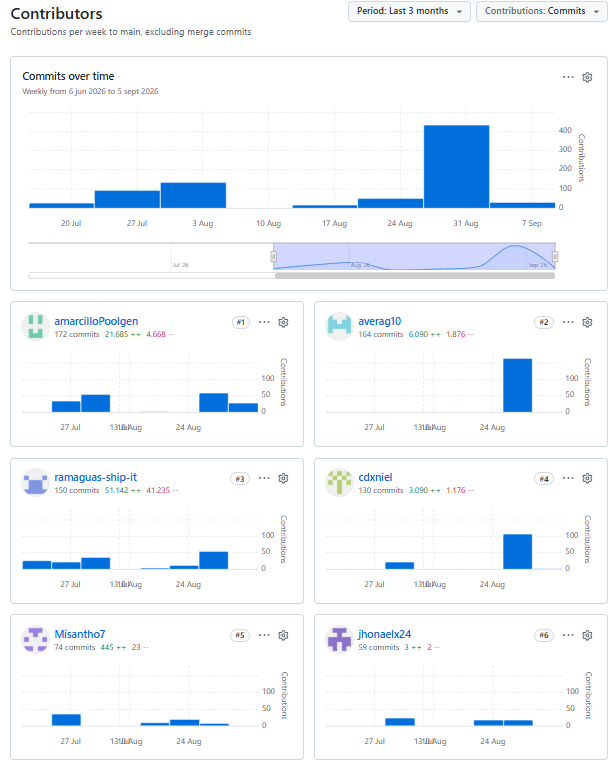
\includegraphics[width=\linewidth,keepaspectratio]{./media/imagen_repositorio.png}
\end{center}

\protect\phantomsection\label{_bookmark115}{}\emph{\textbf{Ilustración 25.
Historial de commits del repositorio}}


\subsection{LISTA DE REQUISITOS CRUDOS
ELICITADOS}\label{lista-de-requisitos-crudos-elicitados}

\begin{quote}
Los siguientes requisitos crudos fueron identificados a partir del
análisis de las dos entrevistas semiestructuradas realizadas y del
análisis del sistema objetivo. Se organizan por área funcional y se
indica la fuente de elicitación para garantizar trazabilidad. La
priorización inicial utiliza el esquema MoSCoW.
\end{quote}

{\def\LTcaptype{none} % do not increment counter
\begin{longtable}[]{@{}
  >{\raggedright\arraybackslash}p{(\linewidth - 8\tabcolsep) * \real{0.0716}}
  >{\raggedright\arraybackslash}p{(\linewidth - 8\tabcolsep) * \real{0.2347}}
  >{\raggedright\arraybackslash}p{(\linewidth - 8\tabcolsep) * \real{0.3814}}
  >{\raggedright\arraybackslash}p{(\linewidth - 8\tabcolsep) * \real{0.1638}}
  >{\raggedright\arraybackslash}p{(\linewidth - 8\tabcolsep) * \real{0.1088}}@{}}
\toprule\noalign{}
\begin{minipage}[b]{\linewidth}\centering
\textbf{ID}
\end{minipage} & \begin{minipage}[b]{\linewidth}\centering
\textbf{Nombre}
\end{minipage} & \begin{minipage}[b]{\linewidth}\centering
\textbf{Descripción}
\end{minipage} & \begin{minipage}[b]{\linewidth}\raggedright
\textbf{Fuente (entrevista)}
\end{minipage} & \begin{minipage}[b]{\linewidth}\centering
\textbf{MoSCoW}
\end{minipage} \\
\midrule\noalign{}
\endhead
\bottomrule\noalign{}
\endlastfoot
\multicolumn{5}{@{}>{\raggedright\arraybackslash}p{(\linewidth - 8\tabcolsep) * \real{0.9603} + 8\tabcolsep}@{}}{%
\textbf{Área 1: Gestión Operativa}} \\
\begin{minipage}[t]{\linewidth}\raggedright
\textbf{RC-01}
\end{minipage} & \begin{minipage}[t]{\linewidth}\raggedright
\textbf{Acceso multiplataforma (móvil y escritorio)}
\end{minipage} & \begin{minipage}[t]{\linewidth}\raggedright
El sistema debe ser accesible desde smartphones (Android/iOS) y
computadoras de escritorio, dado que ambos stakeholders indicaron el
teléfono móvil como dispositivo principal.
\end{minipage} & \begin{minipage}[t]{\linewidth}\raggedright
D3 --- ambas entrevistas
\end{minipage} & \textbf{Must} \\
\begin{minipage}[t]{\linewidth}\raggedright
\textbf{RC-02}
\end{minipage} & \begin{minipage}[t]{\linewidth}\raggedright
\textbf{Centralización de información clínica}
\end{minipage} & \begin{minipage}[t]{\linewidth}\raggedright
El sistema debe centralizar todos los historiales de pacientes (nombre,
edad, raza, peso, diagnósticos, tratamientos) en una única base de datos
consultable.
\end{minipage} & \begin{minipage}[t]{\linewidth}\raggedright
A1/A2 --- Amagua; A1/A2 --- el Veterinario
\end{minipage} & \textbf{Must} \\
\begin{minipage}[t]{\linewidth}\raggedright
\textbf{RC-03}
\end{minipage} & \begin{minipage}[t]{\linewidth}\raggedright
\textbf{Búsqueda rápida por nombre del paciente y nombre del dueño}
\end{minipage} & \begin{minipage}[t]{\linewidth}\raggedright
El sistema debe permitir búsquedas por nombre del animal y por nombre
del propietario para resolver el problema de organización identificado
en Buff Note.
\end{minipage} & \begin{minipage}[t]{\linewidth}\raggedright
A2 --- Amagua ("no está bien organizado el tema de buscar por nombre y dueño")
\end{minipage} & \textbf{Must} \\
\begin{minipage}[t]{\linewidth}\raggedright
\textbf{RC-04}
\end{minipage} & \begin{minipage}[t]{\linewidth}\raggedright
\textbf{Registro detallado de historial clínico}
\end{minipage} & \begin{minipage}[t]{\linewidth}\raggedright
El sistema debe registrar: nombre, edad, raza, peso, motivo de consulta,
diagnóstico, tratamiento, dosis, frecuencia de administración y fecha de cada
consulta.
\end{minipage} & \begin{minipage}[t]{\linewidth}\raggedright
A1 --- Amagua; A2 --- el Veterinario
\end{minipage} & \textbf{Must} \\
\begin{minipage}[t]{\linewidth}\raggedright
\textbf{RC-05}
\end{minipage} & \begin{minipage}[t]{\linewidth}\raggedright
\textbf{Control de inventario con alertas de vencimiento automáticas}
\end{minipage} & \begin{minipage}[t]{\linewidth}\raggedright
El sistema debe registrar cada producto con su fecha de vencimiento y
generar alertas automáticas cuando un producto esté a 30, 15 y 7 días de
su fecha de caducidad.
\end{minipage} & \begin{minipage}[t]{\linewidth}\raggedright
A4 --- el Veterinario ("siempre se caducan por falta de precaución"); A4 --- Amagua
("manualmente revisando uno a uno")
\end{minipage} & \textbf{Must} \\
\begin{minipage}[t]{\linewidth}\raggedright
\textbf{RC-06}
\end{minipage} & \begin{minipage}[t]{\linewidth}\raggedright
\textbf{Gestión de stock con alertas de faltantes}
\end{minipage} & \begin{minipage}[t]{\linewidth}\raggedright
El sistema debe registrar las cantidades en stock y generar alertas
cuando el nivel de un producto caiga por debajo del umbral mínimo configurado.
\end{minipage} & \begin{minipage}[t]{\linewidth}\raggedright
A4 --- ambas entrevistas
\end{minipage} & \textbf{Must} \\
\begin{minipage}[t]{\linewidth}\raggedright
\textbf{RC-07}
\end{minipage} & \begin{minipage}[t]{\linewidth}\raggedright
\textbf{Registro del proceso de cobro}
\end{minipage} & \begin{minipage}[t]{\linewidth}\raggedright
El sistema debe permitir registrar el cobro de cada consulta, incluyendo
los servicios prestados, productos utilizados y monto cobrado.
\end{minipage} & \begin{minipage}[t]{\linewidth}\raggedright
A3 --- el Veterinario; A3 --- Amagua ("la parte más demorada")
\end{minipage} & \textbf{Must} \\
\begin{minipage}[t]{\linewidth}\raggedright
\textbf{RC-08}
\end{minipage} & \begin{minipage}[t]{\linewidth}\raggedright
\textbf{Módulo de facturación ágil}
\end{minipage} & \begin{minipage}[t]{\linewidth}\raggedright
El proceso de registro de una factura no debe requerir más de 3 pasos
desde el inicio hasta la emisión, eliminando las demoras identificadas
en el programa actual.
\end{minipage} & \begin{minipage}[t]{\linewidth}\raggedright
A3 --- Amagua ("es la parte más demorada")
\end{minipage} & \textbf{Must} \\
\begin{minipage}[t]{\linewidth}\raggedright
\textbf{RC-09}
\end{minipage} & \begin{minipage}[t]{\linewidth}\raggedright
\textbf{Registro de comunicaciones post-consulta}
\end{minipage} & \begin{minipage}[t]{\linewidth}\raggedright
El sistema debe registrar las comunicaciones realizadas con los dueños (tipo: llamada, WhatsApp, mensaje), con fecha y resumen del contenido.
\end{minipage} & \begin{minipage}[t]{\linewidth}\raggedright
A6 --- ambas entrevistas
\end{minipage} & Should \\
\begin{minipage}[t]{\linewidth}\raggedright
\textbf{RC-10}
\end{minipage} & \begin{minipage}[t]{\linewidth}\raggedright
\textbf{Envío de resultados por WhatsApp}
\end{minipage} & \begin{minipage}[t]{\linewidth}\raggedright
El sistema debe permitir adjuntar y enviar resultados de exámenes
directamente por WhatsApp desde la plataforma.
\end{minipage} & \begin{minipage}[t]{\linewidth}\raggedright
A6 --- Amagua ("los resultados de exámenes se
\end{minipage} & Should \\
\end{longtable}
}

{\def\LTcaptype{none} % do not increment counter
\begin{longtable}[]{@{}
  >{\raggedright\arraybackslash}p{(\linewidth - 8\tabcolsep) * \real{0.0716}}
  >{\raggedright\arraybackslash}p{(\linewidth - 8\tabcolsep) * \real{0.2347}}
  >{\raggedright\arraybackslash}p{(\linewidth - 8\tabcolsep) * \real{0.3814}}
  >{\raggedright\arraybackslash}p{(\linewidth - 8\tabcolsep) * \real{0.1638}}
  >{\centering\arraybackslash}p{(\linewidth - 8\tabcolsep) * \real{0.1088}}@{}}
\toprule\noalign{}
\begin{minipage}[b]{\linewidth}\raggedright
\end{minipage} & \begin{minipage}[b]{\linewidth}\raggedright
\end{minipage} & \begin{minipage}[b]{\linewidth}\raggedright
\end{minipage} & \begin{minipage}[b]{\linewidth}\raggedright
lo enviamos directamente por WhatsApp")
\end{minipage} & \begin{minipage}[b]{\linewidth}\centering
\end{minipage} \\
\midrule\noalign{}
\endhead
\bottomrule\noalign{}
\endlastfoot
\begin{minipage}[t]{\linewidth}\raggedright
\textbf{RC-11}
\end{minipage} & \begin{minipage}[t]{\linewidth}\raggedright
\textbf{Registro de seguimiento de citas e inasistencias}
\end{minipage} & \begin{minipage}[t]{\linewidth}\raggedright
El sistema debe registrar las citas programadas, las asistencias y las
inasistencias, permitiendo conocer la evolución del paciente incluso
cuando no regresa a control.
\end{minipage} & \begin{minipage}[t]{\linewidth}\raggedright
A5 --- Amagua ("no sabemos qué pasó con el paciente")
\end{minipage} & \textbf{Must} \\
\begin{minipage}[t]{\linewidth}\raggedright
\textbf{RC-12}
\end{minipage} & \begin{minipage}[t]{\linewidth}\raggedright
\textbf{Recordatorios automáticos de citas}
\end{minipage} & \begin{minipage}[t]{\linewidth}\raggedright
El sistema debe enviar recordatorios automáticos (WhatsApp o SMS) al
dueño de la mascota con 24 horas de antelación a una cita programada.
\end{minipage} & \begin{minipage}[t]{\linewidth}\raggedright
A5 --- Amagua; A6 --- el Veterinario
\end{minipage} & Should \\
\multicolumn{5}{@{}>{\raggedright\arraybackslash}p{(\linewidth - 8\tabcolsep) * \real{0.9603} + 8\tabcolsep}@{}}{%
\textbf{Área 2: Seguimiento Clínico y Nutricional}} \\
\begin{minipage}[t]{\linewidth}\raggedright
\textbf{RC-13}
\end{minipage} & \begin{minipage}[t]{\linewidth}\raggedright
\textbf{Registro de parámetros de crecimiento y peso a lo largo del
tiempo}
\end{minipage} & \begin{minipage}[t]{\linewidth}\raggedright
El sistema debe registrar de forma cronológica el peso, edad y
parámetros de condición corporal del animal en cada visita, permitiendo
visualizar tendencias.
\end{minipage} & \begin{minipage}[t]{\linewidth}\raggedright
B1 --- el Veterinario ("en base a la edad va a agarrar el peso"); B1 --- Amagua
\end{minipage} & \textbf{Must} \\
\begin{minipage}[t]{\linewidth}\raggedright
\textbf{RC-14}
\end{minipage} & \begin{minipage}[t]{\linewidth}\raggedright
\textbf{Generación de recomendaciones nutricionales personalizadas}
\end{minipage} & \begin{minipage}[t]{\linewidth}\raggedright
El sistema debe generar recomendaciones de alimentación basadas en la
raza, edad, peso y condición de salud del animal, apoyando el juicio del
veterinario.
\end{minipage} & \begin{minipage}[t]{\linewidth}\raggedright
B2 --- el Veterinario ("inculcarle al dueño del perro la alimentación nutritiva
adecuada"); B2 --- Amagua
\end{minipage} & Should \\
\begin{minipage}[t]{\linewidth}\raggedright
\textbf{RC-15}
\end{minipage} & \begin{minipage}[t]{\linewidth}\raggedright
\textbf{Programación de recordatorios de seguimiento de indicaciones
médicas}
\end{minipage} & \begin{minipage}[t]{\linewidth}\raggedright
El sistema debe permitir programar recordatorios para verificar el
cumplimiento de indicaciones (medicación, dieta, reposo) en fechas
establecidas por el veterinario.
\end{minipage} & \begin{minipage}[t]{\linewidth}\raggedright
B3 --- Amagua ("esperamos que lleguen; si no, no podemos saber")
\end{minipage} & Should \\
\begin{minipage}[t]{\linewidth}\raggedright
\textbf{RC-16}
\end{minipage} & \begin{minipage}[t]{\linewidth}\raggedright
\textbf{Exportación de reportes de salud del paciente}
\end{minipage} & \begin{minipage}[t]{\linewidth}\raggedright
El sistema debe generar y exportar reportes del historial clínico del
paciente en formato PDF para facilitar referencias a clínicas con mayor
equipamiento.
\end{minipage} & \begin{minipage}[t]{\linewidth}\raggedright
B4 --- el Veterinario ("se le indica que hay que hacer pruebas de sangre o llevar a
una clínica con todos los equipos")
\end{minipage} & Should \\
\multicolumn{5}{@{}>{\raggedright\arraybackslash}p{(\linewidth - 8\tabcolsep) * \real{0.9603} + 8\tabcolsep}@{}}{%
\textbf{Área 3: Módulo de Inteligencia Artificial}} \\
\begin{minipage}[t]{\linewidth}\raggedright
\textbf{RC-17}
\end{minipage} & \begin{minipage}[t]{\linewidth}\raggedright
\textbf{Sugerencias diagnósticas basadas en datos clínicos (con
validación obligatoria)}
\end{minipage} & \begin{minipage}[t]{\linewidth}\raggedright
El sistema debe analizar los datos clínicos ingresados por el
veterinario y sugerir posibles diagnósticos diferenciales. Ninguna sugerencia puede aplicarse sin revisión y aprobación explícita
del veterinario.
\end{minipage} & \begin{minipage}[t]{\linewidth}\raggedright
C2/C4 --- Amagua ("si tengo que dar un visto bueno antes, sí"); C4 --- el Veterinario ("confianza moderada")
\end{minipage} & \textbf{Must} \\
\begin{minipage}[t]{\linewidth}\raggedright
\textbf{RC-18}
\end{minipage} & \begin{minipage}[t]{\linewidth}\raggedright
\textbf{Respaldo de recomendaciones en literatura científica veterinaria
validada}
\end{minipage} & \begin{minipage}[t]{\linewidth}\raggedright
Cada sugerencia del módulo de IA debe indicar su fuente bibliográfica
científica para que el veterinario pueda evaluarla.
\end{minipage} & \begin{minipage}[t]{\linewidth}\raggedright
C5 --- ambas entrevistas (primera opción seleccionada en ambos casos)
\end{minipage} & \textbf{Must} \\
\begin{minipage}[t]{\linewidth}\raggedright
\textbf{RC-19}
\end{minipage} & \begin{minipage}[t]{\linewidth}\raggedright
\textbf{Capacidad de revisión y corrección de sugerencias de IA por
parte del veterinario}
\end{minipage} & \begin{minipage}[t]{\linewidth}\raggedright
El sistema debe permitir al veterinario ver, modificar o rechazar
cualquier sugerencia del módulo de IA antes de registrarla en el
historial del paciente.
\end{minipage} & \begin{minipage}[t]{\linewidth}\raggedright
C5 --- Amagua (segunda opción); C5 --- el Veterinario
\end{minipage} & \textbf{Must} \\
\multicolumn{5}{@{}>{\raggedright\arraybackslash}p{(\linewidth - 8\tabcolsep) * \real{0.9603} + 8\tabcolsep}@{}}{%
\textbf{Área 4: Usabilidad, Acceso y Calidad del Sistema}} \\
\end{longtable}
}

{\def\LTcaptype{none} % do not increment counter
\begin{longtable}[]{@{}
  >{\raggedright\arraybackslash}p{(\linewidth - 8\tabcolsep) * \real{0.0716}}
  >{\raggedright\arraybackslash}p{(\linewidth - 8\tabcolsep) * \real{0.2347}}
  >{\raggedright\arraybackslash}p{(\linewidth - 8\tabcolsep) * \real{0.3814}}
  >{\raggedright\arraybackslash}p{(\linewidth - 8\tabcolsep) * \real{0.1638}}
  >{\centering\arraybackslash}p{(\linewidth - 8\tabcolsep) * \real{0.1088}}@{}}
\toprule\noalign{}
\begin{minipage}[b]{\linewidth}\raggedright
\textbf{RC-20}
\end{minipage} & \begin{minipage}[b]{\linewidth}\raggedright
\textbf{Interfaz sencilla sin capacitación prolongada}
\end{minipage} & \begin{minipage}[b]{\linewidth}\raggedright
El sistema debe poder ser utilizado por un veterinario con experiencia
digital básica sin necesidad de un proceso de formación mayor a 2 horas.
\end{minipage} & \begin{minipage}[b]{\linewidth}\raggedright
D2 --- el Veterinario ("que sea fácil de usar"); D2 --- Amagua ("facilidad de utilizarla")
\end{minipage} & \begin{minipage}[b]{\linewidth}\centering
\textbf{Must}
\end{minipage} \\
\midrule\noalign{}
\endhead
\bottomrule\noalign{}
\endlastfoot
\begin{minipage}[t]{\linewidth}\raggedright
\textbf{RC-21}
\end{minipage} & \begin{minipage}[t]{\linewidth}\raggedright
\textbf{Operación con baja dependencia de conectividad permanente}
\end{minipage} & \begin{minipage}[t]{\linewidth}\raggedright
El sistema debe permitir el registro y consulta de historiales clínicos
de manera local cuando no haya conexión a internet, sincronizando
automáticamente al restablecerse la conexión.
\end{minipage} & \begin{minipage}[t]{\linewidth}\raggedright
D4 --- el Veterinario (nivel 2-3/5 de cortes); D4 --- Amagua (rara vez, pero ocurre)
\end{minipage} & Should \\
\begin{minipage}[t]{\linewidth}\raggedright
\textbf{RC-22}
\end{minipage} & \begin{minipage}[t]{\linewidth}\raggedright
\textbf{Bajo costo de implementación y operación}
\end{minipage} & \begin{minipage}[t]{\linewidth}\raggedright
El sistema debe contemplar un modelo de costos accesible para clínicas
de 1 a 3 veterinarios, siendo este un criterio explícito de adopción.
\end{minipage} & \begin{minipage}[t]{\linewidth}\raggedright
D2 --- el Veterinario ("bajo valor económico")
\end{minipage} & \textbf{Must} \\
\begin{minipage}[t]{\linewidth}\raggedright
\textbf{RC-23}
\end{minipage} & \begin{minipage}[t]{\linewidth}\raggedright
\textbf{Perfiles de usuario diferenciados con control de acceso}
\end{minipage} & \begin{minipage}[t]{\linewidth}\raggedright
El sistema debe gestionar al menos dos tipos de perfil de usuario:
médico veterinario y personal administrativo, con accesos y permisos
diferenciados por rol.
\end{minipage} & \begin{minipage}[t]{\linewidth}\raggedright
Sección C/D --- ambas entrevistas; RC identificado por el equipo
\end{minipage} & \textbf{Must} \\
\begin{minipage}[t]{\linewidth}\raggedright
\textbf{RC-24}
\end{minipage} & \begin{minipage}[t]{\linewidth}\raggedright
\textbf{Trazabilidad de cambios en historiales clínicos}
\end{minipage} & \begin{minipage}[t]{\linewidth}\raggedright
El sistema debe registrar automáticamente quién realizó cada
modificación en un historial clínico, con fecha y descripción del cambio.
\end{minipage} & \begin{minipage}[t]{\linewidth}\raggedright
Derivado de RC-04 y RC-17 --- buenas prácticas de IA clínica
\end{minipage} & Should \\
\end{longtable}
}

\protect\phantomsection\label{_bookmark117}{}\emph{\textbf{Tabla 30.
Requisitos crudos elicitados}}

\paragraph{\texorpdfstring{ \ul{Notas de Ajuste respecto al Documento
Proyecto\_1\_vcty}
}{ Notas de Ajuste respecto al Documento Proyecto\_1\_vcty }}\label{notas-de-ajuste-respecto-al-documento-proyecto_1_vcty}

\begin{quote}
En comparación con la lista de requisitos del documento original
(Proyecto\_1\_vcty), se realizaron los siguientes ajustes basados en las
entrevistas reales:
\end{quote}

\begin{itemize}
\item
  RC-03 (NUEVO): Se agregó búsqueda por nombre del dueño además del
  nombre del animal, problema específico identificado por Amagua con
  Buff Note.
\item
  RC-07 y RC-08 (AMPLIADOS): Se separó el registro de cobro (RC-07) de
  la facturación ágil (RC-08), y se añadió el criterio de no más de 3
  pasos basado en el dolor específico de Amagua.
\item
  RC-10 (NUEVO): Envío de resultados por WhatsApp, uso confirmado
  directamente por Amagua.
\item
  RC-17/RC-18/RC-19 (REFINADOS): Los requisitos de IA se desagregaron en
  tres requisitos separados para mayor trazabilidad; la condición de
  validación obligatoria del veterinario es un Must, no un Should.
\item
  RC-21 (AJUSTADO): La operación offline se mantiene como Should (no
  Must) porque Amagua reportó baja frecuencia de cortes (nivel 1-2/5).
\item
  RC-22 (NUEVO): El bajo costo fue mencionado explícitamente como
  criterio de adopción por el Veterinario; se eleva a Must.
\item
  RC original "módulo de configuración para bajo costo" se elimina como
  requisito técnico y se convierte en RC-22 de criterio de negocio.
\end{itemize}

\subsection{REFERENCIAS}\label{referencias-1}

\bibliographystyle{ieeetr}
\bibliography{referencias}

\end{document}